\documentclass[twoside]{book}

% Packages required by doxygen
\usepackage{fixltx2e}
\usepackage{calc}
\usepackage{doxygen}
\usepackage[export]{adjustbox} % also loads graphicx
\usepackage{graphicx}
\usepackage[utf8]{inputenc}
\usepackage{makeidx}
\usepackage{multicol}
\usepackage{multirow}
\PassOptionsToPackage{warn}{textcomp}
\usepackage{textcomp}
\usepackage[nointegrals]{wasysym}
\usepackage[table]{xcolor}

% Font selection
\usepackage[T1]{fontenc}
\usepackage[scaled=.90]{helvet}
\usepackage{courier}
\usepackage{amssymb}
\usepackage{sectsty}
\renewcommand{\familydefault}{\sfdefault}
\allsectionsfont{%
  \fontseries{bc}\selectfont%
  \color{darkgray}%
}
\renewcommand{\DoxyLabelFont}{%
  \fontseries{bc}\selectfont%
  \color{darkgray}%
}
\newcommand{\+}{\discretionary{\mbox{\scriptsize$\hookleftarrow$}}{}{}}

% Page & text layout
\usepackage{geometry}
\geometry{%
  a4paper,%
  top=2.5cm,%
  bottom=2.5cm,%
  left=2.5cm,%
  right=2.5cm%
}
\tolerance=750
\hfuzz=15pt
\hbadness=750
\setlength{\emergencystretch}{15pt}
\setlength{\parindent}{0cm}
\setlength{\parskip}{0.2cm}
\makeatletter
\renewcommand{\paragraph}{%
  \@startsection{paragraph}{4}{0ex}{-1.0ex}{1.0ex}{%
    \normalfont\normalsize\bfseries\SS@parafont%
  }%
}
\renewcommand{\subparagraph}{%
  \@startsection{subparagraph}{5}{0ex}{-1.0ex}{1.0ex}{%
    \normalfont\normalsize\bfseries\SS@subparafont%
  }%
}
\makeatother

% Headers & footers
\usepackage{fancyhdr}
\pagestyle{fancyplain}
\fancyhead[LE]{\fancyplain{}{\bfseries\thepage}}
\fancyhead[CE]{\fancyplain{}{}}
\fancyhead[RE]{\fancyplain{}{\bfseries\leftmark}}
\fancyhead[LO]{\fancyplain{}{\bfseries\rightmark}}
\fancyhead[CO]{\fancyplain{}{}}
\fancyhead[RO]{\fancyplain{}{\bfseries\thepage}}
\fancyfoot[LE]{\fancyplain{}{}}
\fancyfoot[CE]{\fancyplain{}{}}
\fancyfoot[RE]{\fancyplain{}{\bfseries\scriptsize Generated on Sat Jun 13 2015 17\+:43\+:07 for V\+K\+R by Doxygen }}
\fancyfoot[LO]{\fancyplain{}{\bfseries\scriptsize Generated on Sat Jun 13 2015 17\+:43\+:07 for V\+K\+R by Doxygen }}
\fancyfoot[CO]{\fancyplain{}{}}
\fancyfoot[RO]{\fancyplain{}{}}
\renewcommand{\footrulewidth}{0.4pt}
\renewcommand{\chaptermark}[1]{%
  \markboth{#1}{}%
}
\renewcommand{\sectionmark}[1]{%
  \markright{\thesection\ #1}%
}

% Indices & bibliography
\usepackage{natbib}
\usepackage[titles]{tocloft}
\setcounter{tocdepth}{3}
\setcounter{secnumdepth}{5}
\makeindex

% Hyperlinks (required, but should be loaded last)
\usepackage{ifpdf}
\ifpdf
  \usepackage[pdftex,pagebackref=true]{hyperref}
\else
  \usepackage[ps2pdf,pagebackref=true]{hyperref}
\fi
\hypersetup{%
  colorlinks=true,%
  linkcolor=blue,%
  citecolor=blue,%
  unicode%
}

% Custom commands
\newcommand{\clearemptydoublepage}{%
  \newpage{\pagestyle{empty}\cleardoublepage}%
}


%===== C O N T E N T S =====

\begin{document}

% Titlepage & ToC
\hypersetup{pageanchor=false,
             bookmarks=true,
             bookmarksnumbered=true,
             pdfencoding=unicode
            }
\pagenumbering{roman}
\begin{titlepage}
\vspace*{7cm}
\begin{center}%
{\Large V\+K\+R }\\
\vspace*{1cm}
{\large Generated by Doxygen 1.8.9.1}\\
\vspace*{0.5cm}
{\small Sat Jun 13 2015 17:43:07}\\
\end{center}
\end{titlepage}
\clearemptydoublepage
\tableofcontents
\clearemptydoublepage
\pagenumbering{arabic}
\hypersetup{pageanchor=true}

%--- Begin generated contents ---
\chapter{Hierarchical Index}
\section{Class Hierarchy}
This inheritance list is sorted roughly, but not completely, alphabetically\+:\begin{DoxyCompactList}
\item \contentsline{section}{Browseable}{\pageref{classBrowseable}}{}
\item \contentsline{section}{Container}{\pageref{classContainer}}{}
\begin{DoxyCompactList}
\item \contentsline{section}{Lockable\+Container}{\pageref{classLockableContainer}}{}
\end{DoxyCompactList}
\item \contentsline{section}{Generator}{\pageref{classGenerator}}{}
\begin{DoxyCompactList}
\item \contentsline{section}{Cpp\+Generator}{\pageref{classCppGenerator}}{}
\item \contentsline{section}{Java\+Generator}{\pageref{classJavaGenerator}}{}
\item \contentsline{section}{Obj\+Pascal\+Generator}{\pageref{classObjPascalGenerator}}{}
\item \contentsline{section}{Pascal\+Generator}{\pageref{classPascalGenerator}}{}
\end{DoxyCompactList}
\item \contentsline{section}{Method\+Type\+Info}{\pageref{structMethodTypeInfo}}{}
\item \contentsline{section}{Model}{\pageref{classModel}}{}
\item \contentsline{section}{Model\+Member}{\pageref{classModelMember}}{}
\item \contentsline{section}{Movable}{\pageref{classMovable}}{}
\item \contentsline{section}{N\+\_\+\+Model}{\pageref{classN__Model}}{}
\item \contentsline{section}{N\+\_\+\+Model\+Member}{\pageref{classN__ModelMember}}{}
\begin{DoxyCompactList}
\item \contentsline{section}{N\+\_\+\+Class\+Member}{\pageref{classN__ClassMember}}{}
\begin{DoxyCompactList}
\item \contentsline{section}{N\+\_\+\+Field}{\pageref{classN__Field}}{}
\begin{DoxyCompactList}
\item \contentsline{section}{N\+\_\+\+Param}{\pageref{classN__Param}}{}
\end{DoxyCompactList}
\item \contentsline{section}{N\+\_\+\+Method}{\pageref{classN__Method}}{}
\begin{DoxyCompactList}
\item \contentsline{section}{N\+\_\+\+Constructor}{\pageref{classN__Constructor}}{}
\item \contentsline{section}{N\+\_\+\+Destructor}{\pageref{classN__Destructor}}{}
\end{DoxyCompactList}
\end{DoxyCompactList}
\item \contentsline{section}{N\+\_\+\+Interface}{\pageref{classN__Interface}}{}
\begin{DoxyCompactList}
\item \contentsline{section}{N\+\_\+\+Class}{\pageref{classN__Class}}{}
\begin{DoxyCompactList}
\item \contentsline{section}{N\+\_\+\+Exception}{\pageref{classN__Exception}}{}
\end{DoxyCompactList}
\end{DoxyCompactList}
\item \contentsline{section}{N\+\_\+\+Model\+Option}{\pageref{classN__ModelOption}}{}
\item \contentsline{section}{N\+\_\+\+Type}{\pageref{classN__Type}}{}
\end{DoxyCompactList}
\item \contentsline{section}{yy\+\_\+buffer\+\_\+state}{\pageref{structyy__buffer__state}}{}
\item \contentsline{section}{yy\+\_\+trans\+\_\+info}{\pageref{structyy__trans__info}}{}
\item \contentsline{section}{yyalloc}{\pageref{unionyyalloc}}{}
\item \contentsline{section}{Y\+Y\+S\+T\+Y\+P\+E}{\pageref{unionYYSTYPE}}{}
\end{DoxyCompactList}

\chapter{Class Index}
\section{Class List}
Here are the classes, structs, unions and interfaces with brief descriptions\+:\begin{DoxyCompactList}
\item\contentsline{section}{\hyperlink{classBrowseable}{Browseable} }{\pageref{classBrowseable}}{}
\item\contentsline{section}{\hyperlink{classContainer}{Container} }{\pageref{classContainer}}{}
\item\contentsline{section}{\hyperlink{classCppGenerator}{Cpp\+Generator} }{\pageref{classCppGenerator}}{}
\item\contentsline{section}{\hyperlink{classGenerator}{Generator} }{\pageref{classGenerator}}{}
\item\contentsline{section}{\hyperlink{classJavaGenerator}{Java\+Generator} }{\pageref{classJavaGenerator}}{}
\item\contentsline{section}{\hyperlink{classLockableContainer}{Lockable\+Container} }{\pageref{classLockableContainer}}{}
\item\contentsline{section}{\hyperlink{structMethodTypeInfo}{Method\+Type\+Info} }{\pageref{structMethodTypeInfo}}{}
\item\contentsline{section}{\hyperlink{classModel}{Model} }{\pageref{classModel}}{}
\item\contentsline{section}{\hyperlink{classModelMember}{Model\+Member} }{\pageref{classModelMember}}{}
\item\contentsline{section}{\hyperlink{classMovable}{Movable} }{\pageref{classMovable}}{}
\item\contentsline{section}{\hyperlink{classN__Class}{N\+\_\+\+Class} }{\pageref{classN__Class}}{}
\item\contentsline{section}{\hyperlink{classN__ClassMember}{N\+\_\+\+Class\+Member} }{\pageref{classN__ClassMember}}{}
\item\contentsline{section}{\hyperlink{classN__Constructor}{N\+\_\+\+Constructor} }{\pageref{classN__Constructor}}{}
\item\contentsline{section}{\hyperlink{classN__Destructor}{N\+\_\+\+Destructor} }{\pageref{classN__Destructor}}{}
\item\contentsline{section}{\hyperlink{classN__Exception}{N\+\_\+\+Exception} }{\pageref{classN__Exception}}{}
\item\contentsline{section}{\hyperlink{classN__Field}{N\+\_\+\+Field} }{\pageref{classN__Field}}{}
\item\contentsline{section}{\hyperlink{classN__Interface}{N\+\_\+\+Interface} }{\pageref{classN__Interface}}{}
\item\contentsline{section}{\hyperlink{classN__Method}{N\+\_\+\+Method} }{\pageref{classN__Method}}{}
\item\contentsline{section}{\hyperlink{classN__Model}{N\+\_\+\+Model} }{\pageref{classN__Model}}{}
\item\contentsline{section}{\hyperlink{classN__ModelMember}{N\+\_\+\+Model\+Member} }{\pageref{classN__ModelMember}}{}
\item\contentsline{section}{\hyperlink{classN__ModelOption}{N\+\_\+\+Model\+Option} }{\pageref{classN__ModelOption}}{}
\item\contentsline{section}{\hyperlink{classN__Param}{N\+\_\+\+Param} }{\pageref{classN__Param}}{}
\item\contentsline{section}{\hyperlink{classN__Type}{N\+\_\+\+Type} }{\pageref{classN__Type}}{}
\item\contentsline{section}{\hyperlink{classObjPascalGenerator}{Obj\+Pascal\+Generator} }{\pageref{classObjPascalGenerator}}{}
\item\contentsline{section}{\hyperlink{classPascalGenerator}{Pascal\+Generator} }{\pageref{classPascalGenerator}}{}
\item\contentsline{section}{\hyperlink{structyy__buffer__state}{yy\+\_\+buffer\+\_\+state} }{\pageref{structyy__buffer__state}}{}
\item\contentsline{section}{\hyperlink{structyy__trans__info}{yy\+\_\+trans\+\_\+info} }{\pageref{structyy__trans__info}}{}
\item\contentsline{section}{\hyperlink{unionyyalloc}{yyalloc} }{\pageref{unionyyalloc}}{}
\item\contentsline{section}{\hyperlink{unionYYSTYPE}{Y\+Y\+S\+T\+Y\+P\+E} }{\pageref{unionYYSTYPE}}{}
\end{DoxyCompactList}

\chapter{File Index}
\section{File List}
Here is a list of all files with brief descriptions\+:\begin{DoxyCompactList}
\item\contentsline{section}{\hyperlink{ast_8cpp}{ast.\+cpp} }{\pageref{ast_8cpp}}{}
\item\contentsline{section}{\hyperlink{ast_8h}{ast.\+h} }{\pageref{ast_8h}}{}
\item\contentsline{section}{\hyperlink{lex_8yy_8c}{lex.\+yy.\+c} }{\pageref{lex_8yy_8c}}{}
\item\contentsline{section}{\hyperlink{main_8cpp}{main.\+cpp} }{\pageref{main_8cpp}}{}
\item\contentsline{section}{\hyperlink{parser_8cpp}{parser.\+cpp} }{\pageref{parser_8cpp}}{}
\item\contentsline{section}{\hyperlink{parser_8hpp}{parser.\+hpp} }{\pageref{parser_8hpp}}{}
\item\contentsline{section}{\hyperlink{TestModel_8cc}{Test\+Model.\+cc} }{\pageref{TestModel_8cc}}{}
\item\contentsline{section}{\hyperlink{TestModel_8h}{Test\+Model.\+h} }{\pageref{TestModel_8h}}{}
\item\contentsline{section}{\hyperlink{util_8cpp}{util.\+cpp} }{\pageref{util_8cpp}}{}
\item\contentsline{section}{\hyperlink{util_8h}{util.\+h} }{\pageref{util_8h}}{}
\end{DoxyCompactList}

\chapter{Class Documentation}
\hypertarget{classBrowseable}{}\section{Browseable Class Reference}
\label{classBrowseable}\index{Browseable@{Browseable}}


{\ttfamily \#include $<$Test\+Model.\+h$>$}

\subsection*{Public Member Functions}
\begin{DoxyCompactItemize}
\item 
\hyperlink{TestModel_8h_a8bcef75446d80c7fb35ff8ab36f5cbb5}{content\+\_\+type\+\_\+t} \hyperlink{classBrowseable_a67a97605df654d7534ee7e5cdb1e754f}{browse} ()=0  throw (\+Locked\+Exception)
\end{DoxyCompactItemize}


\subsection{Member Function Documentation}
\hypertarget{classBrowseable_a67a97605df654d7534ee7e5cdb1e754f}{}\index{Browseable@{Browseable}!browse@{browse}}
\index{browse@{browse}!Browseable@{Browseable}}
\subsubsection[{browse}]{\setlength{\rightskip}{0pt plus 5cm}{\bf content\+\_\+type\+\_\+t} Browseable\+::browse (
\begin{DoxyParamCaption}
{}
\end{DoxyParamCaption}
) throw  Locked\+Exception) \hspace{0.3cm}{\ttfamily [pure virtual]}}\label{classBrowseable_a67a97605df654d7534ee7e5cdb1e754f}


The documentation for this class was generated from the following file\+:\begin{DoxyCompactItemize}
\item 
\hyperlink{TestModel_8h}{Test\+Model.\+h}\end{DoxyCompactItemize}

\hypertarget{classContainer}{}\section{Container Class Reference}
\label{classContainer}\index{Container@{Container}}


{\ttfamily \#include $<$Test\+Model.\+h$>$}

Inheritance diagram for Container\+:\begin{figure}[H]
\begin{center}
\leavevmode
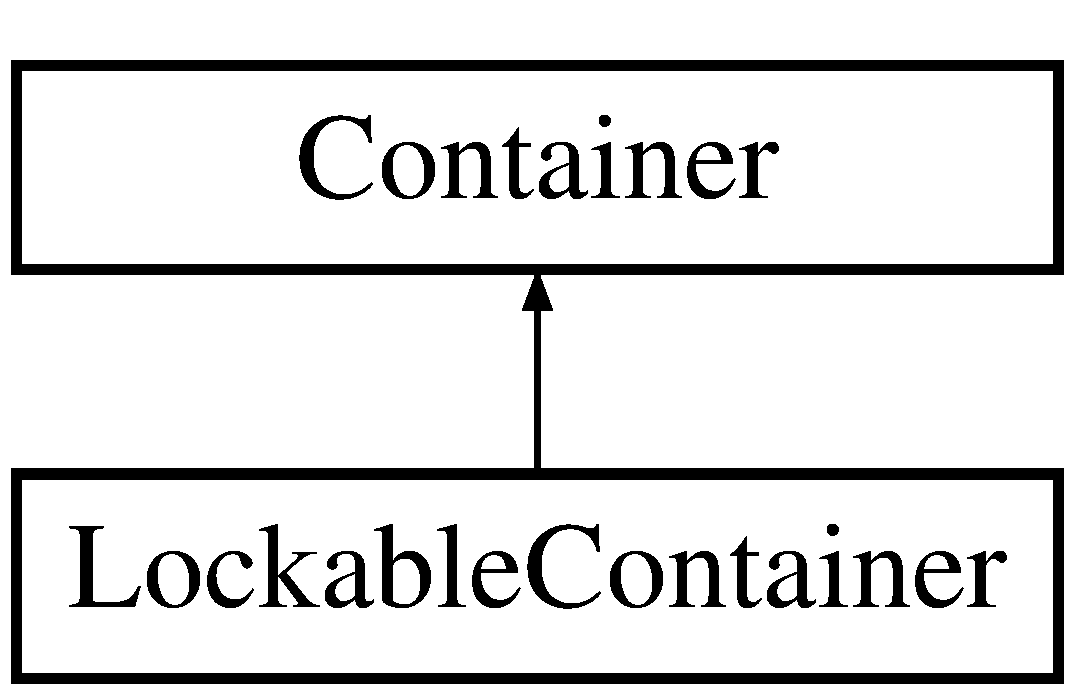
\includegraphics[height=2.000000cm]{classContainer}
\end{center}
\end{figure}


The documentation for this class was generated from the following file\+:\begin{DoxyCompactItemize}
\item 
\hyperlink{TestModel_8h}{Test\+Model.\+h}\end{DoxyCompactItemize}

\hypertarget{classCppGenerator}{}\section{Cpp\+Generator Class Reference}
\label{classCppGenerator}\index{Cpp\+Generator@{Cpp\+Generator}}


{\ttfamily \#include $<$ast.\+h$>$}

Inheritance diagram for Cpp\+Generator\+:\begin{figure}[H]
\begin{center}
\leavevmode
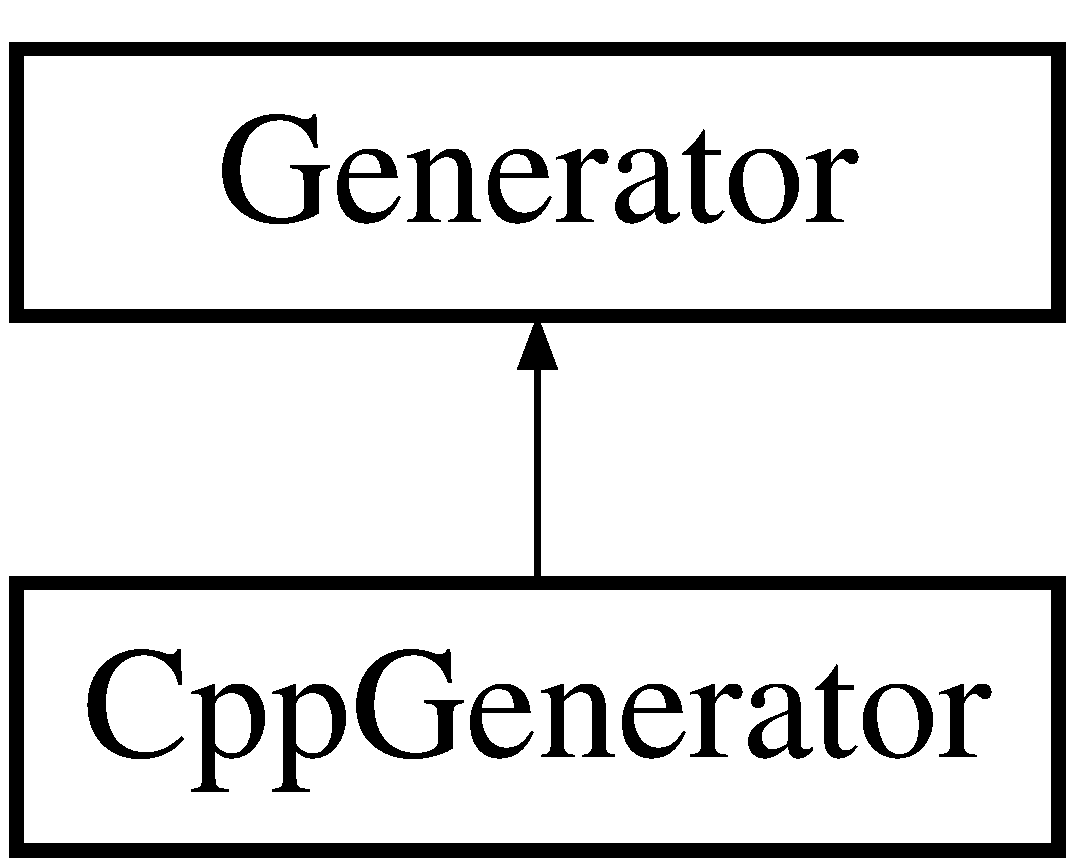
\includegraphics[height=2.000000cm]{classCppGenerator}
\end{center}
\end{figure}
\subsection*{Public Member Functions}
\begin{DoxyCompactItemize}
\item 
virtual \hyperlink{classCppGenerator_ab81a7eddeeb169492b8885f8b39e669e}{$\sim$\+Cpp\+Generator} ()
\item 
virtual void \hyperlink{classCppGenerator_a32c3cf7f72e81b52b6937a1dcaef865d}{generate} (\hyperlink{classN__Model}{N\+\_\+\+Model} \&m)
\item 
virtual std\+::string \hyperlink{classCppGenerator_a0befaf088820c9e3b9432457f9c775db}{gen\+Interface} (\hyperlink{classN__Interface}{N\+\_\+\+Interface} $\ast$c)
\item 
virtual std\+::string \hyperlink{classCppGenerator_aedb02142a2bcdd47dc6575d317ce5408}{gen\+Field} (\hyperlink{classN__Field}{N\+\_\+\+Field} $\ast$f)
\item 
virtual std\+::string \hyperlink{classCppGenerator_a25aeb086603decc6941c8a02c52ad90e}{gen\+Method} (\hyperlink{classN__Method}{N\+\_\+\+Method} $\ast$m)
\item 
virtual std\+::string \hyperlink{classCppGenerator_ad4cf3df3310368d485dac04a41505028}{gen\+Method\+Header} (\hyperlink{classN__Method}{N\+\_\+\+Method} $\ast$m)
\item 
virtual std\+::string \hyperlink{classCppGenerator_a7a0eb0f95cb897e3f702279b3df2f47a}{gen\+Parameter} (\hyperlink{classN__Param}{N\+\_\+\+Param} $\ast$p)
\item 
virtual std\+::string \hyperlink{classCppGenerator_aff63ea51beb1daf7e6ec0c72628e9e6f}{gen\+Class} (\hyperlink{classN__Class}{N\+\_\+\+Class} $\ast$c)
\end{DoxyCompactItemize}
\subsection*{Protected Member Functions}
\begin{DoxyCompactItemize}
\item 
\hyperlink{classCppGenerator_ae6aa3030be1678a05bac49f27c3415ec}{Cpp\+Generator} (std\+::ostream \&os)
\end{DoxyCompactItemize}
\subsection*{Friends}
\begin{DoxyCompactItemize}
\item 
class \hyperlink{classCppGenerator_a366b7823e659ab78d952a7d79662a4d6}{Generator}
\end{DoxyCompactItemize}
\subsection*{Additional Inherited Members}


\subsection{Detailed Description}
Генератор кода на C++ 

\subsection{Constructor \& Destructor Documentation}
\hypertarget{classCppGenerator_ae6aa3030be1678a05bac49f27c3415ec}{}\index{Cpp\+Generator@{Cpp\+Generator}!Cpp\+Generator@{Cpp\+Generator}}
\index{Cpp\+Generator@{Cpp\+Generator}!Cpp\+Generator@{Cpp\+Generator}}
\subsubsection[{Cpp\+Generator}]{\setlength{\rightskip}{0pt plus 5cm}Cpp\+Generator\+::\+Cpp\+Generator (
\begin{DoxyParamCaption}
\item[{std\+::ostream \&}]{os}
\end{DoxyParamCaption}
)\hspace{0.3cm}{\ttfamily [inline]}, {\ttfamily [protected]}}\label{classCppGenerator_ae6aa3030be1678a05bac49f27c3415ec}
Конструктор 
\begin{DoxyParams}{Parameters}
{\em os} & -\/ поток, в который необходимо выдавать шаблон \\
\hline
\end{DoxyParams}
\hypertarget{classCppGenerator_ab81a7eddeeb169492b8885f8b39e669e}{}\index{Cpp\+Generator@{Cpp\+Generator}!````~Cpp\+Generator@{$\sim$\+Cpp\+Generator}}
\index{````~Cpp\+Generator@{$\sim$\+Cpp\+Generator}!Cpp\+Generator@{Cpp\+Generator}}
\subsubsection[{$\sim$\+Cpp\+Generator}]{\setlength{\rightskip}{0pt plus 5cm}virtual Cpp\+Generator\+::$\sim$\+Cpp\+Generator (
\begin{DoxyParamCaption}
{}
\end{DoxyParamCaption}
)\hspace{0.3cm}{\ttfamily [inline]}, {\ttfamily [virtual]}}\label{classCppGenerator_ab81a7eddeeb169492b8885f8b39e669e}


\subsection{Member Function Documentation}
\hypertarget{classCppGenerator_aff63ea51beb1daf7e6ec0c72628e9e6f}{}\index{Cpp\+Generator@{Cpp\+Generator}!gen\+Class@{gen\+Class}}
\index{gen\+Class@{gen\+Class}!Cpp\+Generator@{Cpp\+Generator}}
\subsubsection[{gen\+Class}]{\setlength{\rightskip}{0pt plus 5cm}std\+::string Cpp\+Generator\+::gen\+Class (
\begin{DoxyParamCaption}
\item[{{\bf N\+\_\+\+Class} $\ast$}]{c}
\end{DoxyParamCaption}
)\hspace{0.3cm}{\ttfamily [virtual]}}\label{classCppGenerator_aff63ea51beb1daf7e6ec0c72628e9e6f}
Генератор шаблона класса 
\begin{DoxyParams}{Parameters}
{\em c} & -\/ класс, для которого необходимо сгенерировать шаблон \\
\hline
\end{DoxyParams}
\begin{DoxyReturn}{Returns}
Сгенерированный шаблон 
\end{DoxyReturn}


Implements \hyperlink{classGenerator_afac361fceae302fb09e8170d097415d4}{Generator}.

\hypertarget{classCppGenerator_a32c3cf7f72e81b52b6937a1dcaef865d}{}\index{Cpp\+Generator@{Cpp\+Generator}!generate@{generate}}
\index{generate@{generate}!Cpp\+Generator@{Cpp\+Generator}}
\subsubsection[{generate}]{\setlength{\rightskip}{0pt plus 5cm}void Cpp\+Generator\+::generate (
\begin{DoxyParamCaption}
\item[{{\bf N\+\_\+\+Model} \&}]{m}
\end{DoxyParamCaption}
)\hspace{0.3cm}{\ttfamily [virtual]}}\label{classCppGenerator_a32c3cf7f72e81b52b6937a1dcaef865d}
Генератор шаблона модели 
\begin{DoxyParams}{Parameters}
{\em m} & -\/ модель, для которой необходимо сгенерировать шаблон \\
\hline
\end{DoxyParams}


Implements \hyperlink{classGenerator_a518161ca79e68d733687f8e2985abd16}{Generator}.

\hypertarget{classCppGenerator_aedb02142a2bcdd47dc6575d317ce5408}{}\index{Cpp\+Generator@{Cpp\+Generator}!gen\+Field@{gen\+Field}}
\index{gen\+Field@{gen\+Field}!Cpp\+Generator@{Cpp\+Generator}}
\subsubsection[{gen\+Field}]{\setlength{\rightskip}{0pt plus 5cm}std\+::string Cpp\+Generator\+::gen\+Field (
\begin{DoxyParamCaption}
\item[{{\bf N\+\_\+\+Field} $\ast$}]{f}
\end{DoxyParamCaption}
)\hspace{0.3cm}{\ttfamily [virtual]}}\label{classCppGenerator_aedb02142a2bcdd47dc6575d317ce5408}
Генератор шаблона поля класса 
\begin{DoxyParams}{Parameters}
{\em f} & -\/ поле, для которого необходимо сгенерировать шаблон \\
\hline
\end{DoxyParams}
\begin{DoxyReturn}{Returns}
Сгенерированный шаблон 
\end{DoxyReturn}


Implements \hyperlink{classGenerator_aa2871c303fba42abd61a7ed997d23416}{Generator}.

\hypertarget{classCppGenerator_a0befaf088820c9e3b9432457f9c775db}{}\index{Cpp\+Generator@{Cpp\+Generator}!gen\+Interface@{gen\+Interface}}
\index{gen\+Interface@{gen\+Interface}!Cpp\+Generator@{Cpp\+Generator}}
\subsubsection[{gen\+Interface}]{\setlength{\rightskip}{0pt plus 5cm}std\+::string Cpp\+Generator\+::gen\+Interface (
\begin{DoxyParamCaption}
\item[{{\bf N\+\_\+\+Interface} $\ast$}]{c}
\end{DoxyParamCaption}
)\hspace{0.3cm}{\ttfamily [virtual]}}\label{classCppGenerator_a0befaf088820c9e3b9432457f9c775db}
Генератор шаблона интерфейса 
\begin{DoxyParams}{Parameters}
{\em c} & -\/ интерфейс, для которого необходимо сгенерировать шаблон \\
\hline
\end{DoxyParams}
\begin{DoxyReturn}{Returns}
Сгенерированный шаблон 
\end{DoxyReturn}


Implements \hyperlink{classGenerator_ad0f09fcc0e99e78e04f8c202cd0ce881}{Generator}.

\hypertarget{classCppGenerator_a25aeb086603decc6941c8a02c52ad90e}{}\index{Cpp\+Generator@{Cpp\+Generator}!gen\+Method@{gen\+Method}}
\index{gen\+Method@{gen\+Method}!Cpp\+Generator@{Cpp\+Generator}}
\subsubsection[{gen\+Method}]{\setlength{\rightskip}{0pt plus 5cm}std\+::string Cpp\+Generator\+::gen\+Method (
\begin{DoxyParamCaption}
\item[{{\bf N\+\_\+\+Method} $\ast$}]{m}
\end{DoxyParamCaption}
)\hspace{0.3cm}{\ttfamily [virtual]}}\label{classCppGenerator_a25aeb086603decc6941c8a02c52ad90e}
Генератор шаблона метода 
\begin{DoxyParams}{Parameters}
{\em m} & -\/ метод, для которого необходимо сгенерировать шаблон \\
\hline
\end{DoxyParams}
\begin{DoxyReturn}{Returns}
Сгенерированный шаблон 
\end{DoxyReturn}


Implements \hyperlink{classGenerator_a2b09ae359674038af5286fbd03d83c41}{Generator}.

\hypertarget{classCppGenerator_ad4cf3df3310368d485dac04a41505028}{}\index{Cpp\+Generator@{Cpp\+Generator}!gen\+Method\+Header@{gen\+Method\+Header}}
\index{gen\+Method\+Header@{gen\+Method\+Header}!Cpp\+Generator@{Cpp\+Generator}}
\subsubsection[{gen\+Method\+Header}]{\setlength{\rightskip}{0pt plus 5cm}std\+::string Cpp\+Generator\+::gen\+Method\+Header (
\begin{DoxyParamCaption}
\item[{{\bf N\+\_\+\+Method} $\ast$}]{m}
\end{DoxyParamCaption}
)\hspace{0.3cm}{\ttfamily [virtual]}}\label{classCppGenerator_ad4cf3df3310368d485dac04a41505028}
Генератор шаблона заголовка метода 
\begin{DoxyParams}{Parameters}
{\em m} & -\/ метод, для которого необходимо сгенерировать шаблон \\
\hline
\end{DoxyParams}
\begin{DoxyReturn}{Returns}
Сгенерированный шаблон 
\end{DoxyReturn}


Implements \hyperlink{classGenerator_aede7f5343c5bcd88b5fc8bfe51d17bce}{Generator}.

\hypertarget{classCppGenerator_a7a0eb0f95cb897e3f702279b3df2f47a}{}\index{Cpp\+Generator@{Cpp\+Generator}!gen\+Parameter@{gen\+Parameter}}
\index{gen\+Parameter@{gen\+Parameter}!Cpp\+Generator@{Cpp\+Generator}}
\subsubsection[{gen\+Parameter}]{\setlength{\rightskip}{0pt plus 5cm}std\+::string Cpp\+Generator\+::gen\+Parameter (
\begin{DoxyParamCaption}
\item[{{\bf N\+\_\+\+Param} $\ast$}]{p}
\end{DoxyParamCaption}
)\hspace{0.3cm}{\ttfamily [virtual]}}\label{classCppGenerator_a7a0eb0f95cb897e3f702279b3df2f47a}
Генератор шаблона параметра метода 
\begin{DoxyParams}{Parameters}
{\em p} & -\/ параметр, для которого необходимо сгенерировать шаблон \\
\hline
\end{DoxyParams}
\begin{DoxyReturn}{Returns}
Сгенерированный шаблон 
\end{DoxyReturn}


Implements \hyperlink{classGenerator_ac9871b3d5874cb81a98a3e5eb3b703e2}{Generator}.



\subsection{Friends And Related Function Documentation}
\hypertarget{classCppGenerator_a366b7823e659ab78d952a7d79662a4d6}{}\index{Cpp\+Generator@{Cpp\+Generator}!Generator@{Generator}}
\index{Generator@{Generator}!Cpp\+Generator@{Cpp\+Generator}}
\subsubsection[{Generator}]{\setlength{\rightskip}{0pt plus 5cm}friend class {\bf Generator}\hspace{0.3cm}{\ttfamily [friend]}}\label{classCppGenerator_a366b7823e659ab78d952a7d79662a4d6}


The documentation for this class was generated from the following files\+:\begin{DoxyCompactItemize}
\item 
\hyperlink{ast_8h}{ast.\+h}\item 
\hyperlink{ast_8cpp}{ast.\+cpp}\end{DoxyCompactItemize}

\hypertarget{classGenerator}{}\section{Generator Class Reference}
\label{classGenerator}\index{Generator@{Generator}}


{\ttfamily \#include $<$ast.\+h$>$}

Inheritance diagram for Generator\+:\begin{figure}[H]
\begin{center}
\leavevmode
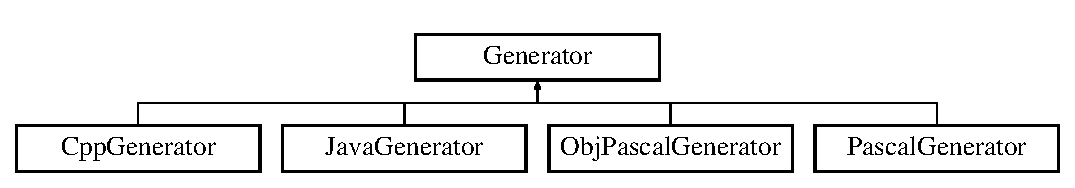
\includegraphics[height=2.000000cm]{classGenerator}
\end{center}
\end{figure}
\subsection*{Public Member Functions}
\begin{DoxyCompactItemize}
\item 
virtual void \hyperlink{classGenerator_a518161ca79e68d733687f8e2985abd16}{generate} (\hyperlink{classN__Model}{N\+\_\+\+Model} \&m)=0
\item 
virtual std\+::string \hyperlink{classGenerator_ad0f09fcc0e99e78e04f8c202cd0ce881}{gen\+Interface} (\hyperlink{classN__Interface}{N\+\_\+\+Interface} $\ast$c)=0
\item 
virtual std\+::string \hyperlink{classGenerator_aa2871c303fba42abd61a7ed997d23416}{gen\+Field} (\hyperlink{classN__Field}{N\+\_\+\+Field} $\ast$f)=0
\item 
virtual std\+::string \hyperlink{classGenerator_a2b09ae359674038af5286fbd03d83c41}{gen\+Method} (\hyperlink{classN__Method}{N\+\_\+\+Method} $\ast$m)=0
\item 
virtual std\+::string \hyperlink{classGenerator_aede7f5343c5bcd88b5fc8bfe51d17bce}{gen\+Method\+Header} (\hyperlink{classN__Method}{N\+\_\+\+Method} $\ast$m)=0
\item 
virtual std\+::string \hyperlink{classGenerator_ac9871b3d5874cb81a98a3e5eb3b703e2}{gen\+Parameter} (\hyperlink{classN__Param}{N\+\_\+\+Param} $\ast$p)=0
\item 
virtual std\+::string \hyperlink{classGenerator_afac361fceae302fb09e8170d097415d4}{gen\+Class} (\hyperlink{classN__Class}{N\+\_\+\+Class} $\ast$c)=0
\item 
virtual \hyperlink{classGenerator_aeb355d65ed59bc5738a5b3e9637186e1}{$\sim$\+Generator} ()
\end{DoxyCompactItemize}
\subsection*{Static Public Member Functions}
\begin{DoxyCompactItemize}
\item 
static \hyperlink{classGenerator}{Generator} $\ast$ \hyperlink{classGenerator_a8a97794e699a220d5833589d966eb28b}{create} (\hyperlink{ast_8h_a315ca917ad583797f709ea477dd28705}{Language} lang, std\+::ostream \&os)
\end{DoxyCompactItemize}
\subsection*{Protected Member Functions}
\begin{DoxyCompactItemize}
\item 
\hyperlink{classGenerator_a28efb1004a6a78f811a4d7b74f568169}{Generator} (std\+::ostream \&os)
\end{DoxyCompactItemize}
\subsection*{Protected Attributes}
\begin{DoxyCompactItemize}
\item 
std\+::ostream \& \hyperlink{classGenerator_a66fe842aa93b878a74c96fb0852d4626}{m\+\_\+os}
\begin{DoxyCompactList}\small\item\em Поток вывода шаблона \end{DoxyCompactList}\end{DoxyCompactItemize}
\subsection*{Friends}
\begin{DoxyCompactItemize}
\item 
std\+::ostream \& \hyperlink{classGenerator_a5b6ac73277bce0e06ed614d1202031e1}{operator$<$$<$} (\hyperlink{classGenerator}{Generator} \&os, const \hyperlink{classN__ModelMember}{N\+\_\+\+Model\+Member} \&mm)
\end{DoxyCompactItemize}


\subsection{Detailed Description}
Абстрактный класс генератора шаблона кода 

\subsection{Constructor \& Destructor Documentation}
\hypertarget{classGenerator_a28efb1004a6a78f811a4d7b74f568169}{}\index{Generator@{Generator}!Generator@{Generator}}
\index{Generator@{Generator}!Generator@{Generator}}
\subsubsection[{Generator}]{\setlength{\rightskip}{0pt plus 5cm}Generator\+::\+Generator (
\begin{DoxyParamCaption}
\item[{std\+::ostream \&}]{os}
\end{DoxyParamCaption}
)\hspace{0.3cm}{\ttfamily [inline]}, {\ttfamily [explicit]}, {\ttfamily [protected]}}\label{classGenerator_a28efb1004a6a78f811a4d7b74f568169}
Конструктор 
\begin{DoxyParams}{Parameters}
{\em os} & -\/ поток, в который необходимо выдавать шаблон \\
\hline
\end{DoxyParams}
\hypertarget{classGenerator_aeb355d65ed59bc5738a5b3e9637186e1}{}\index{Generator@{Generator}!````~Generator@{$\sim$\+Generator}}
\index{````~Generator@{$\sim$\+Generator}!Generator@{Generator}}
\subsubsection[{$\sim$\+Generator}]{\setlength{\rightskip}{0pt plus 5cm}virtual Generator\+::$\sim$\+Generator (
\begin{DoxyParamCaption}
{}
\end{DoxyParamCaption}
)\hspace{0.3cm}{\ttfamily [inline]}, {\ttfamily [virtual]}}\label{classGenerator_aeb355d65ed59bc5738a5b3e9637186e1}
Деструктор 

\subsection{Member Function Documentation}
\hypertarget{classGenerator_a8a97794e699a220d5833589d966eb28b}{}\index{Generator@{Generator}!create@{create}}
\index{create@{create}!Generator@{Generator}}
\subsubsection[{create}]{\setlength{\rightskip}{0pt plus 5cm}{\bf Generator} $\ast$ Generator\+::create (
\begin{DoxyParamCaption}
\item[{{\bf Language}}]{lang, }
\item[{std\+::ostream \&}]{os}
\end{DoxyParamCaption}
)\hspace{0.3cm}{\ttfamily [static]}}\label{classGenerator_a8a97794e699a220d5833589d966eb28b}
Классовый метод для создания экземпляра генератора 
\begin{DoxyParams}{Parameters}
{\em lang} & -\/ язык, для которого требуется создать генератор \\
\hline
{\em os} & -\/ поток вывода, в который предполагается выводить шаблон \\
\hline
\end{DoxyParams}
\begin{DoxyReturn}{Returns}
Экземпляр генератора 
\end{DoxyReturn}
\hypertarget{classGenerator_afac361fceae302fb09e8170d097415d4}{}\index{Generator@{Generator}!gen\+Class@{gen\+Class}}
\index{gen\+Class@{gen\+Class}!Generator@{Generator}}
\subsubsection[{gen\+Class}]{\setlength{\rightskip}{0pt plus 5cm}virtual std\+::string Generator\+::gen\+Class (
\begin{DoxyParamCaption}
\item[{{\bf N\+\_\+\+Class} $\ast$}]{c}
\end{DoxyParamCaption}
)\hspace{0.3cm}{\ttfamily [pure virtual]}}\label{classGenerator_afac361fceae302fb09e8170d097415d4}
Генератор шаблона класса 
\begin{DoxyParams}{Parameters}
{\em c} & -\/ класс, для которого необходимо сгенерировать шаблон \\
\hline
\end{DoxyParams}
\begin{DoxyReturn}{Returns}
Сгенерированный шаблон 
\end{DoxyReturn}


Implemented in \hyperlink{classObjPascalGenerator_a690ce15adcc6d94fc994737f1acdfac7}{Obj\+Pascal\+Generator}, \hyperlink{classPascalGenerator_ae8bf162efb54e857c9a61bf9aae5f6e4}{Pascal\+Generator}, \hyperlink{classJavaGenerator_afe0fee40e5af2729afaae8b392c7e0db}{Java\+Generator}, and \hyperlink{classCppGenerator_aff63ea51beb1daf7e6ec0c72628e9e6f}{Cpp\+Generator}.

\hypertarget{classGenerator_a518161ca79e68d733687f8e2985abd16}{}\index{Generator@{Generator}!generate@{generate}}
\index{generate@{generate}!Generator@{Generator}}
\subsubsection[{generate}]{\setlength{\rightskip}{0pt plus 5cm}virtual void Generator\+::generate (
\begin{DoxyParamCaption}
\item[{{\bf N\+\_\+\+Model} \&}]{m}
\end{DoxyParamCaption}
)\hspace{0.3cm}{\ttfamily [pure virtual]}}\label{classGenerator_a518161ca79e68d733687f8e2985abd16}
Генератор шаблона модели 
\begin{DoxyParams}{Parameters}
{\em m} & -\/ модель, для которой необходимо сгенерировать шаблон \\
\hline
\end{DoxyParams}


Implemented in \hyperlink{classObjPascalGenerator_a8129a8aab5c9b1f8dab3bb3c4de460d0}{Obj\+Pascal\+Generator}, \hyperlink{classPascalGenerator_af0d2d3b1fbf63c8c4859b446541337c5}{Pascal\+Generator}, \hyperlink{classJavaGenerator_a9a920fcd472a9afd7eb44fb5f76d60af}{Java\+Generator}, and \hyperlink{classCppGenerator_a32c3cf7f72e81b52b6937a1dcaef865d}{Cpp\+Generator}.

\hypertarget{classGenerator_aa2871c303fba42abd61a7ed997d23416}{}\index{Generator@{Generator}!gen\+Field@{gen\+Field}}
\index{gen\+Field@{gen\+Field}!Generator@{Generator}}
\subsubsection[{gen\+Field}]{\setlength{\rightskip}{0pt plus 5cm}virtual std\+::string Generator\+::gen\+Field (
\begin{DoxyParamCaption}
\item[{{\bf N\+\_\+\+Field} $\ast$}]{f}
\end{DoxyParamCaption}
)\hspace{0.3cm}{\ttfamily [pure virtual]}}\label{classGenerator_aa2871c303fba42abd61a7ed997d23416}
Генератор шаблона поля класса 
\begin{DoxyParams}{Parameters}
{\em f} & -\/ поле, для которого необходимо сгенерировать шаблон \\
\hline
\end{DoxyParams}
\begin{DoxyReturn}{Returns}
Сгенерированный шаблон 
\end{DoxyReturn}


Implemented in \hyperlink{classObjPascalGenerator_a0bb3fad2c4df2a741c96d37d1e2d4449}{Obj\+Pascal\+Generator}, \hyperlink{classPascalGenerator_a2518deea7c307b53d2f5569653772df4}{Pascal\+Generator}, \hyperlink{classJavaGenerator_ac86377f3b08c88d53ee1669c8b623f8e}{Java\+Generator}, and \hyperlink{classCppGenerator_aedb02142a2bcdd47dc6575d317ce5408}{Cpp\+Generator}.

\hypertarget{classGenerator_ad0f09fcc0e99e78e04f8c202cd0ce881}{}\index{Generator@{Generator}!gen\+Interface@{gen\+Interface}}
\index{gen\+Interface@{gen\+Interface}!Generator@{Generator}}
\subsubsection[{gen\+Interface}]{\setlength{\rightskip}{0pt plus 5cm}virtual std\+::string Generator\+::gen\+Interface (
\begin{DoxyParamCaption}
\item[{{\bf N\+\_\+\+Interface} $\ast$}]{c}
\end{DoxyParamCaption}
)\hspace{0.3cm}{\ttfamily [pure virtual]}}\label{classGenerator_ad0f09fcc0e99e78e04f8c202cd0ce881}
Генератор шаблона интерфейса 
\begin{DoxyParams}{Parameters}
{\em c} & -\/ интерфейс, для которого необходимо сгенерировать шаблон \\
\hline
\end{DoxyParams}
\begin{DoxyReturn}{Returns}
Сгенерированный шаблон 
\end{DoxyReturn}


Implemented in \hyperlink{classObjPascalGenerator_a833b2caffb9da2595a9f447bc6264ecf}{Obj\+Pascal\+Generator}, \hyperlink{classPascalGenerator_a45d98b0d7ee0cba9708bbce1cc6e81a8}{Pascal\+Generator}, \hyperlink{classJavaGenerator_a08be7bd01581127d1d6b7f1ca388aa8c}{Java\+Generator}, and \hyperlink{classCppGenerator_a0befaf088820c9e3b9432457f9c775db}{Cpp\+Generator}.

\hypertarget{classGenerator_a2b09ae359674038af5286fbd03d83c41}{}\index{Generator@{Generator}!gen\+Method@{gen\+Method}}
\index{gen\+Method@{gen\+Method}!Generator@{Generator}}
\subsubsection[{gen\+Method}]{\setlength{\rightskip}{0pt plus 5cm}virtual std\+::string Generator\+::gen\+Method (
\begin{DoxyParamCaption}
\item[{{\bf N\+\_\+\+Method} $\ast$}]{m}
\end{DoxyParamCaption}
)\hspace{0.3cm}{\ttfamily [pure virtual]}}\label{classGenerator_a2b09ae359674038af5286fbd03d83c41}
Генератор шаблона метода 
\begin{DoxyParams}{Parameters}
{\em m} & -\/ метод, для которого необходимо сгенерировать шаблон \\
\hline
\end{DoxyParams}
\begin{DoxyReturn}{Returns}
Сгенерированный шаблон 
\end{DoxyReturn}


Implemented in \hyperlink{classObjPascalGenerator_a4fa9c56ef03cc1999ce178fabedebb60}{Obj\+Pascal\+Generator}, \hyperlink{classPascalGenerator_a676b9e2ca462c770d6eab2cd9150d078}{Pascal\+Generator}, \hyperlink{classJavaGenerator_af49a575754a670af62b8c38a87c62383}{Java\+Generator}, and \hyperlink{classCppGenerator_a25aeb086603decc6941c8a02c52ad90e}{Cpp\+Generator}.

\hypertarget{classGenerator_aede7f5343c5bcd88b5fc8bfe51d17bce}{}\index{Generator@{Generator}!gen\+Method\+Header@{gen\+Method\+Header}}
\index{gen\+Method\+Header@{gen\+Method\+Header}!Generator@{Generator}}
\subsubsection[{gen\+Method\+Header}]{\setlength{\rightskip}{0pt plus 5cm}virtual std\+::string Generator\+::gen\+Method\+Header (
\begin{DoxyParamCaption}
\item[{{\bf N\+\_\+\+Method} $\ast$}]{m}
\end{DoxyParamCaption}
)\hspace{0.3cm}{\ttfamily [pure virtual]}}\label{classGenerator_aede7f5343c5bcd88b5fc8bfe51d17bce}
Генератор шаблона заголовка метода 
\begin{DoxyParams}{Parameters}
{\em m} & -\/ метод, для которого необходимо сгенерировать шаблон \\
\hline
\end{DoxyParams}
\begin{DoxyReturn}{Returns}
Сгенерированный шаблон 
\end{DoxyReturn}


Implemented in \hyperlink{classObjPascalGenerator_a1c6095fef516716336de164da25da1e2}{Obj\+Pascal\+Generator}, \hyperlink{classPascalGenerator_a588bf9c593871ccf52f5ab66d2b25258}{Pascal\+Generator}, \hyperlink{classJavaGenerator_af69f42b427c011da412d987ca5b87bd5}{Java\+Generator}, and \hyperlink{classCppGenerator_ad4cf3df3310368d485dac04a41505028}{Cpp\+Generator}.

\hypertarget{classGenerator_ac9871b3d5874cb81a98a3e5eb3b703e2}{}\index{Generator@{Generator}!gen\+Parameter@{gen\+Parameter}}
\index{gen\+Parameter@{gen\+Parameter}!Generator@{Generator}}
\subsubsection[{gen\+Parameter}]{\setlength{\rightskip}{0pt plus 5cm}virtual std\+::string Generator\+::gen\+Parameter (
\begin{DoxyParamCaption}
\item[{{\bf N\+\_\+\+Param} $\ast$}]{p}
\end{DoxyParamCaption}
)\hspace{0.3cm}{\ttfamily [pure virtual]}}\label{classGenerator_ac9871b3d5874cb81a98a3e5eb3b703e2}
Генератор шаблона параметра метода 
\begin{DoxyParams}{Parameters}
{\em p} & -\/ параметр, для которого необходимо сгенерировать шаблон \\
\hline
\end{DoxyParams}
\begin{DoxyReturn}{Returns}
Сгенерированный шаблон 
\end{DoxyReturn}


Implemented in \hyperlink{classObjPascalGenerator_a1f6ec48b26e0a002816737220a6eb26d}{Obj\+Pascal\+Generator}, \hyperlink{classPascalGenerator_a4498120ec4549002fb575316f1f58257}{Pascal\+Generator}, \hyperlink{classJavaGenerator_a3431b1f8d251ab7a5a45ee3e809213ff}{Java\+Generator}, and \hyperlink{classCppGenerator_a7a0eb0f95cb897e3f702279b3df2f47a}{Cpp\+Generator}.



\subsection{Friends And Related Function Documentation}
\hypertarget{classGenerator_a5b6ac73277bce0e06ed614d1202031e1}{}\index{Generator@{Generator}!operator$<$$<$@{operator$<$$<$}}
\index{operator$<$$<$@{operator$<$$<$}!Generator@{Generator}}
\subsubsection[{operator$<$$<$}]{\setlength{\rightskip}{0pt plus 5cm}std\+::ostream\& operator$<$$<$ (
\begin{DoxyParamCaption}
\item[{{\bf Generator} \&}]{os, }
\item[{const {\bf N\+\_\+\+Model\+Member} \&}]{mm}
\end{DoxyParamCaption}
)\hspace{0.3cm}{\ttfamily [friend]}}\label{classGenerator_a5b6ac73277bce0e06ed614d1202031e1}
Оператор вывода компонента модели в поток вывода шаблона 
\begin{DoxyParams}{Parameters}
{\em os} & -\/ поток вывода, в который выводится шаблон компонента модели \\
\hline
{\em mm} & -\/ выводимый компонент модели \\
\hline
\end{DoxyParams}
\begin{DoxyReturn}{Returns}
Поток вывода, в который был выведен шаблон 
\end{DoxyReturn}


\subsection{Member Data Documentation}
\hypertarget{classGenerator_a66fe842aa93b878a74c96fb0852d4626}{}\index{Generator@{Generator}!m\+\_\+os@{m\+\_\+os}}
\index{m\+\_\+os@{m\+\_\+os}!Generator@{Generator}}
\subsubsection[{m\+\_\+os}]{\setlength{\rightskip}{0pt plus 5cm}std\+::ostream\& Generator\+::m\+\_\+os\hspace{0.3cm}{\ttfamily [protected]}}\label{classGenerator_a66fe842aa93b878a74c96fb0852d4626}


Поток вывода шаблона 



The documentation for this class was generated from the following files\+:\begin{DoxyCompactItemize}
\item 
\hyperlink{ast_8h}{ast.\+h}\item 
\hyperlink{ast_8cpp}{ast.\+cpp}\end{DoxyCompactItemize}

\hypertarget{classJavaGenerator}{}\section{Java\+Generator Class Reference}
\label{classJavaGenerator}\index{Java\+Generator@{Java\+Generator}}


{\ttfamily \#include $<$ast.\+h$>$}

Inheritance diagram for Java\+Generator\+:\begin{figure}[H]
\begin{center}
\leavevmode
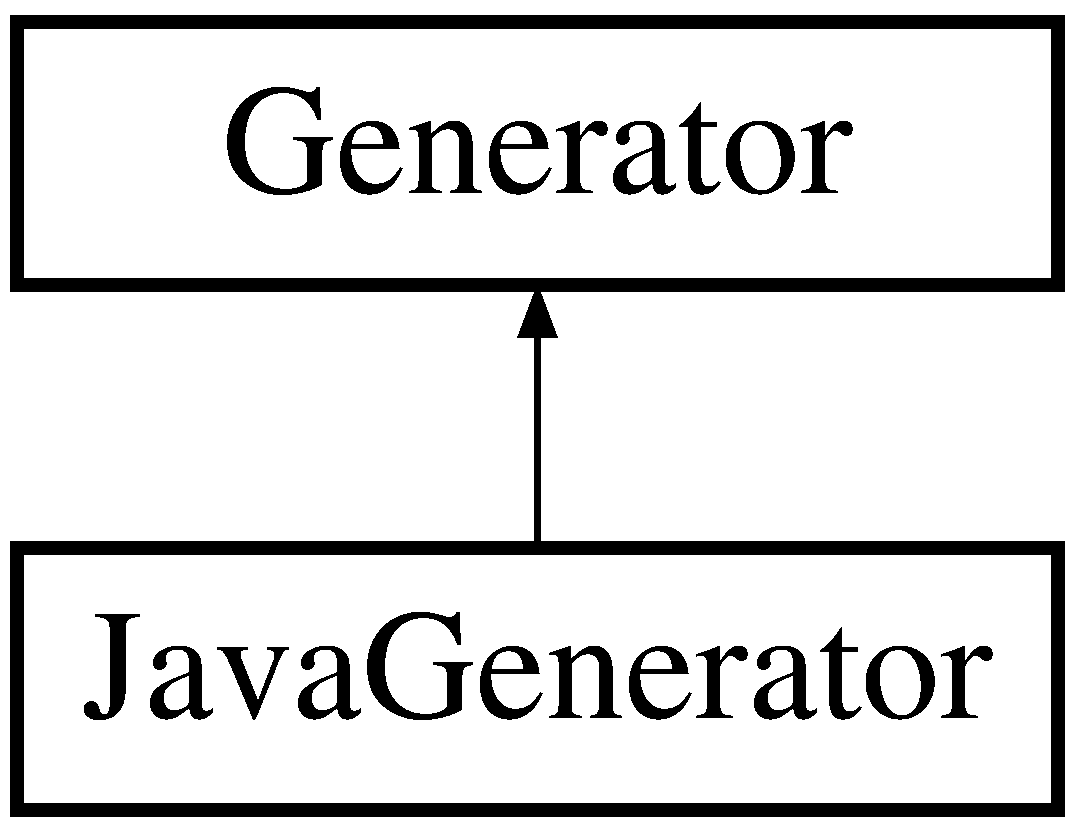
\includegraphics[height=2.000000cm]{classJavaGenerator}
\end{center}
\end{figure}
\subsection*{Public Member Functions}
\begin{DoxyCompactItemize}
\item 
virtual \hyperlink{classJavaGenerator_abe76750a970b9dcdd25c6c9192df835e}{$\sim$\+Java\+Generator} ()
\item 
virtual void \hyperlink{classJavaGenerator_a9a920fcd472a9afd7eb44fb5f76d60af}{generate} (\hyperlink{classN__Model}{N\+\_\+\+Model} \&m)
\item 
virtual std\+::string \hyperlink{classJavaGenerator_a08be7bd01581127d1d6b7f1ca388aa8c}{gen\+Interface} (\hyperlink{classN__Interface}{N\+\_\+\+Interface} $\ast$c)
\item 
virtual std\+::string \hyperlink{classJavaGenerator_ac86377f3b08c88d53ee1669c8b623f8e}{gen\+Field} (\hyperlink{classN__Field}{N\+\_\+\+Field} $\ast$f)
\item 
virtual std\+::string \hyperlink{classJavaGenerator_af49a575754a670af62b8c38a87c62383}{gen\+Method} (\hyperlink{classN__Method}{N\+\_\+\+Method} $\ast$m)
\item 
virtual std\+::string \hyperlink{classJavaGenerator_af69f42b427c011da412d987ca5b87bd5}{gen\+Method\+Header} (\hyperlink{classN__Method}{N\+\_\+\+Method} $\ast$m)
\item 
virtual std\+::string \hyperlink{classJavaGenerator_a3431b1f8d251ab7a5a45ee3e809213ff}{gen\+Parameter} (\hyperlink{classN__Param}{N\+\_\+\+Param} $\ast$p)
\item 
virtual std\+::string \hyperlink{classJavaGenerator_afe0fee40e5af2729afaae8b392c7e0db}{gen\+Class} (\hyperlink{classN__Class}{N\+\_\+\+Class} $\ast$c)
\end{DoxyCompactItemize}
\subsection*{Protected Member Functions}
\begin{DoxyCompactItemize}
\item 
\hyperlink{classJavaGenerator_ac7274498d758221f160aced6ba3e62f8}{Java\+Generator} (std\+::ostream \&os)
\end{DoxyCompactItemize}
\subsection*{Friends}
\begin{DoxyCompactItemize}
\item 
class \hyperlink{classJavaGenerator_a366b7823e659ab78d952a7d79662a4d6}{Generator}
\end{DoxyCompactItemize}
\subsection*{Additional Inherited Members}


\subsection{Detailed Description}
Генератор кода на Java 

\subsection{Constructor \& Destructor Documentation}
\hypertarget{classJavaGenerator_ac7274498d758221f160aced6ba3e62f8}{}\index{Java\+Generator@{Java\+Generator}!Java\+Generator@{Java\+Generator}}
\index{Java\+Generator@{Java\+Generator}!Java\+Generator@{Java\+Generator}}
\subsubsection[{Java\+Generator}]{\setlength{\rightskip}{0pt plus 5cm}Java\+Generator\+::\+Java\+Generator (
\begin{DoxyParamCaption}
\item[{std\+::ostream \&}]{os}
\end{DoxyParamCaption}
)\hspace{0.3cm}{\ttfamily [inline]}, {\ttfamily [protected]}}\label{classJavaGenerator_ac7274498d758221f160aced6ba3e62f8}
\hypertarget{classJavaGenerator_abe76750a970b9dcdd25c6c9192df835e}{}\index{Java\+Generator@{Java\+Generator}!````~Java\+Generator@{$\sim$\+Java\+Generator}}
\index{````~Java\+Generator@{$\sim$\+Java\+Generator}!Java\+Generator@{Java\+Generator}}
\subsubsection[{$\sim$\+Java\+Generator}]{\setlength{\rightskip}{0pt plus 5cm}virtual Java\+Generator\+::$\sim$\+Java\+Generator (
\begin{DoxyParamCaption}
{}
\end{DoxyParamCaption}
)\hspace{0.3cm}{\ttfamily [inline]}, {\ttfamily [virtual]}}\label{classJavaGenerator_abe76750a970b9dcdd25c6c9192df835e}


\subsection{Member Function Documentation}
\hypertarget{classJavaGenerator_afe0fee40e5af2729afaae8b392c7e0db}{}\index{Java\+Generator@{Java\+Generator}!gen\+Class@{gen\+Class}}
\index{gen\+Class@{gen\+Class}!Java\+Generator@{Java\+Generator}}
\subsubsection[{gen\+Class}]{\setlength{\rightskip}{0pt plus 5cm}std\+::string Java\+Generator\+::gen\+Class (
\begin{DoxyParamCaption}
\item[{{\bf N\+\_\+\+Class} $\ast$}]{c}
\end{DoxyParamCaption}
)\hspace{0.3cm}{\ttfamily [virtual]}}\label{classJavaGenerator_afe0fee40e5af2729afaae8b392c7e0db}
Генератор шаблона класса 
\begin{DoxyParams}{Parameters}
{\em c} & -\/ класс, для которого необходимо сгенерировать шаблон \\
\hline
\end{DoxyParams}
\begin{DoxyReturn}{Returns}
Сгенерированный шаблон 
\end{DoxyReturn}


Implements \hyperlink{classGenerator_afac361fceae302fb09e8170d097415d4}{Generator}.

\hypertarget{classJavaGenerator_a9a920fcd472a9afd7eb44fb5f76d60af}{}\index{Java\+Generator@{Java\+Generator}!generate@{generate}}
\index{generate@{generate}!Java\+Generator@{Java\+Generator}}
\subsubsection[{generate}]{\setlength{\rightskip}{0pt plus 5cm}void Java\+Generator\+::generate (
\begin{DoxyParamCaption}
\item[{{\bf N\+\_\+\+Model} \&}]{m}
\end{DoxyParamCaption}
)\hspace{0.3cm}{\ttfamily [virtual]}}\label{classJavaGenerator_a9a920fcd472a9afd7eb44fb5f76d60af}
Генератор шаблона модели 
\begin{DoxyParams}{Parameters}
{\em m} & -\/ модель, для которой необходимо сгенерировать шаблон \\
\hline
\end{DoxyParams}


Implements \hyperlink{classGenerator_a518161ca79e68d733687f8e2985abd16}{Generator}.

\hypertarget{classJavaGenerator_ac86377f3b08c88d53ee1669c8b623f8e}{}\index{Java\+Generator@{Java\+Generator}!gen\+Field@{gen\+Field}}
\index{gen\+Field@{gen\+Field}!Java\+Generator@{Java\+Generator}}
\subsubsection[{gen\+Field}]{\setlength{\rightskip}{0pt plus 5cm}std\+::string Java\+Generator\+::gen\+Field (
\begin{DoxyParamCaption}
\item[{{\bf N\+\_\+\+Field} $\ast$}]{f}
\end{DoxyParamCaption}
)\hspace{0.3cm}{\ttfamily [virtual]}}\label{classJavaGenerator_ac86377f3b08c88d53ee1669c8b623f8e}
Генератор шаблона поля класса 
\begin{DoxyParams}{Parameters}
{\em f} & -\/ поле, для которого необходимо сгенерировать шаблон \\
\hline
\end{DoxyParams}
\begin{DoxyReturn}{Returns}
Сгенерированный шаблон 
\end{DoxyReturn}


Implements \hyperlink{classGenerator_aa2871c303fba42abd61a7ed997d23416}{Generator}.

\hypertarget{classJavaGenerator_a08be7bd01581127d1d6b7f1ca388aa8c}{}\index{Java\+Generator@{Java\+Generator}!gen\+Interface@{gen\+Interface}}
\index{gen\+Interface@{gen\+Interface}!Java\+Generator@{Java\+Generator}}
\subsubsection[{gen\+Interface}]{\setlength{\rightskip}{0pt plus 5cm}std\+::string Java\+Generator\+::gen\+Interface (
\begin{DoxyParamCaption}
\item[{{\bf N\+\_\+\+Interface} $\ast$}]{c}
\end{DoxyParamCaption}
)\hspace{0.3cm}{\ttfamily [virtual]}}\label{classJavaGenerator_a08be7bd01581127d1d6b7f1ca388aa8c}
Генератор шаблона интерфейса 
\begin{DoxyParams}{Parameters}
{\em c} & -\/ интерфейс, для которого необходимо сгенерировать шаблон \\
\hline
\end{DoxyParams}
\begin{DoxyReturn}{Returns}
Сгенерированный шаблон 
\end{DoxyReturn}


Implements \hyperlink{classGenerator_ad0f09fcc0e99e78e04f8c202cd0ce881}{Generator}.

\hypertarget{classJavaGenerator_af49a575754a670af62b8c38a87c62383}{}\index{Java\+Generator@{Java\+Generator}!gen\+Method@{gen\+Method}}
\index{gen\+Method@{gen\+Method}!Java\+Generator@{Java\+Generator}}
\subsubsection[{gen\+Method}]{\setlength{\rightskip}{0pt plus 5cm}std\+::string Java\+Generator\+::gen\+Method (
\begin{DoxyParamCaption}
\item[{{\bf N\+\_\+\+Method} $\ast$}]{m}
\end{DoxyParamCaption}
)\hspace{0.3cm}{\ttfamily [virtual]}}\label{classJavaGenerator_af49a575754a670af62b8c38a87c62383}
Генератор шаблона метода 
\begin{DoxyParams}{Parameters}
{\em m} & -\/ метод, для которого необходимо сгенерировать шаблон \\
\hline
\end{DoxyParams}
\begin{DoxyReturn}{Returns}
Сгенерированный шаблон 
\end{DoxyReturn}


Implements \hyperlink{classGenerator_a2b09ae359674038af5286fbd03d83c41}{Generator}.

\hypertarget{classJavaGenerator_af69f42b427c011da412d987ca5b87bd5}{}\index{Java\+Generator@{Java\+Generator}!gen\+Method\+Header@{gen\+Method\+Header}}
\index{gen\+Method\+Header@{gen\+Method\+Header}!Java\+Generator@{Java\+Generator}}
\subsubsection[{gen\+Method\+Header}]{\setlength{\rightskip}{0pt plus 5cm}std\+::string Java\+Generator\+::gen\+Method\+Header (
\begin{DoxyParamCaption}
\item[{{\bf N\+\_\+\+Method} $\ast$}]{m}
\end{DoxyParamCaption}
)\hspace{0.3cm}{\ttfamily [virtual]}}\label{classJavaGenerator_af69f42b427c011da412d987ca5b87bd5}
Генератор шаблона заголовка метода 
\begin{DoxyParams}{Parameters}
{\em m} & -\/ метод, для которого необходимо сгенерировать шаблон \\
\hline
\end{DoxyParams}
\begin{DoxyReturn}{Returns}
Сгенерированный шаблон 
\end{DoxyReturn}


Implements \hyperlink{classGenerator_aede7f5343c5bcd88b5fc8bfe51d17bce}{Generator}.

\hypertarget{classJavaGenerator_a3431b1f8d251ab7a5a45ee3e809213ff}{}\index{Java\+Generator@{Java\+Generator}!gen\+Parameter@{gen\+Parameter}}
\index{gen\+Parameter@{gen\+Parameter}!Java\+Generator@{Java\+Generator}}
\subsubsection[{gen\+Parameter}]{\setlength{\rightskip}{0pt plus 5cm}std\+::string Java\+Generator\+::gen\+Parameter (
\begin{DoxyParamCaption}
\item[{{\bf N\+\_\+\+Param} $\ast$}]{p}
\end{DoxyParamCaption}
)\hspace{0.3cm}{\ttfamily [virtual]}}\label{classJavaGenerator_a3431b1f8d251ab7a5a45ee3e809213ff}
Генератор шаблона параметра метода 
\begin{DoxyParams}{Parameters}
{\em p} & -\/ параметр, для которого необходимо сгенерировать шаблон \\
\hline
\end{DoxyParams}
\begin{DoxyReturn}{Returns}
Сгенерированный шаблон 
\end{DoxyReturn}


Implements \hyperlink{classGenerator_ac9871b3d5874cb81a98a3e5eb3b703e2}{Generator}.



\subsection{Friends And Related Function Documentation}
\hypertarget{classJavaGenerator_a366b7823e659ab78d952a7d79662a4d6}{}\index{Java\+Generator@{Java\+Generator}!Generator@{Generator}}
\index{Generator@{Generator}!Java\+Generator@{Java\+Generator}}
\subsubsection[{Generator}]{\setlength{\rightskip}{0pt plus 5cm}friend class {\bf Generator}\hspace{0.3cm}{\ttfamily [friend]}}\label{classJavaGenerator_a366b7823e659ab78d952a7d79662a4d6}


The documentation for this class was generated from the following files\+:\begin{DoxyCompactItemize}
\item 
\hyperlink{ast_8h}{ast.\+h}\item 
\hyperlink{ast_8cpp}{ast.\+cpp}\end{DoxyCompactItemize}

\hypertarget{classLockableContainer}{}\section{Lockable\+Container Class Reference}
\label{classLockableContainer}\index{Lockable\+Container@{Lockable\+Container}}


{\ttfamily \#include $<$Test\+Model.\+h$>$}

Inheritance diagram for Lockable\+Container\+:\begin{figure}[H]
\begin{center}
\leavevmode
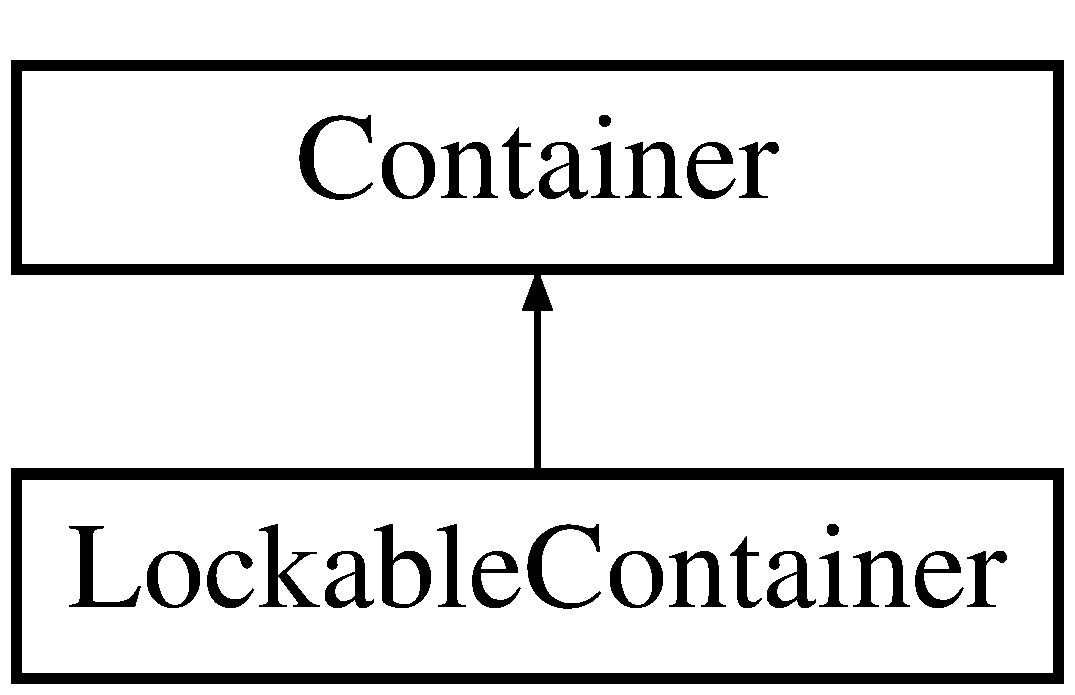
\includegraphics[height=2.000000cm]{classLockableContainer}
\end{center}
\end{figure}


The documentation for this class was generated from the following file\+:\begin{DoxyCompactItemize}
\item 
\hyperlink{TestModel_8h}{Test\+Model.\+h}\end{DoxyCompactItemize}

\hypertarget{structMethodTypeInfo}{}\section{Method\+Type\+Info Struct Reference}
\label{structMethodTypeInfo}\index{Method\+Type\+Info@{Method\+Type\+Info}}


{\ttfamily \#include $<$ast.\+h$>$}

\subsection*{Public Attributes}
\begin{DoxyCompactItemize}
\item 
std\+::string $\ast$ \hyperlink{structMethodTypeInfo_a4bd6ddafdf47413038f62af796fe816a}{return\+\_\+type}
\begin{DoxyCompactList}\small\item\em Тип возвращаемого значения \end{DoxyCompactList}\item 
\hyperlink{ast_8h_a3006a5b9309b36eaa1cf179f1478b0cd}{Method\+Type} \hyperlink{structMethodTypeInfo_a27d1fc69f1b76fd1b0958e0791dcc1e0}{method\+\_\+type}
\begin{DoxyCompactList}\small\item\em Тип метода \end{DoxyCompactList}\end{DoxyCompactItemize}


\subsection{Detailed Description}
Информация о типе метода 

\subsection{Member Data Documentation}
\hypertarget{structMethodTypeInfo_a27d1fc69f1b76fd1b0958e0791dcc1e0}{}\index{Method\+Type\+Info@{Method\+Type\+Info}!method\+\_\+type@{method\+\_\+type}}
\index{method\+\_\+type@{method\+\_\+type}!Method\+Type\+Info@{Method\+Type\+Info}}
\subsubsection[{method\+\_\+type}]{\setlength{\rightskip}{0pt plus 5cm}{\bf Method\+Type} Method\+Type\+Info\+::method\+\_\+type}\label{structMethodTypeInfo_a27d1fc69f1b76fd1b0958e0791dcc1e0}


Тип метода 

\hypertarget{structMethodTypeInfo_a4bd6ddafdf47413038f62af796fe816a}{}\index{Method\+Type\+Info@{Method\+Type\+Info}!return\+\_\+type@{return\+\_\+type}}
\index{return\+\_\+type@{return\+\_\+type}!Method\+Type\+Info@{Method\+Type\+Info}}
\subsubsection[{return\+\_\+type}]{\setlength{\rightskip}{0pt plus 5cm}std\+::string$\ast$ Method\+Type\+Info\+::return\+\_\+type}\label{structMethodTypeInfo_a4bd6ddafdf47413038f62af796fe816a}


Тип возвращаемого значения 



The documentation for this struct was generated from the following file\+:\begin{DoxyCompactItemize}
\item 
\hyperlink{ast_8h}{ast.\+h}\end{DoxyCompactItemize}

\hypertarget{classModel}{}\section{Model Class Reference}
\label{classModel}\index{Model@{Model}}


{\ttfamily \#include $<$ast.\+h$>$}



\subsection{Detailed Description}
Классовая модель, корневой узел 

The documentation for this class was generated from the following file\+:\begin{DoxyCompactItemize}
\item 
\hyperlink{ast_8h}{ast.\+h}\end{DoxyCompactItemize}

\hypertarget{classModelMember}{}\section{Model\+Member Class Reference}
\label{classModelMember}\index{Model\+Member@{Model\+Member}}


{\ttfamily \#include $<$ast.\+h$>$}



\subsection{Detailed Description}
Произвольный элемент модели 

The documentation for this class was generated from the following file\+:\begin{DoxyCompactItemize}
\item 
\hyperlink{ast_8h}{ast.\+h}\end{DoxyCompactItemize}

\hypertarget{classMovable}{}\section{Movable Class Reference}
\label{classMovable}\index{Movable@{Movable}}


{\ttfamily \#include $<$Test\+Model.\+h$>$}

\subsection*{Public Member Functions}
\begin{DoxyCompactItemize}
\item 
int \hyperlink{classMovable_a9f9c8a3ba344ad6301cc2f7324ca108b}{get\+X} ()=0
\item 
int \hyperlink{classMovable_a8bf1a487559414a1e48f39a398b0704d}{get\+Y} ()=0
\item 
void \hyperlink{classMovable_a6f5638435e40dc166b1fba5a192265c1}{get\+X\+Y} (int \&x, int \&y)=0
\item 
void \hyperlink{classMovable_a97ded74028dc55af2ed292e52c4045a7}{set\+X\+Y} (int x, int y)=0
\item 
void \hyperlink{classMovable_a951f140708d98ff486e7b6dd5526f100}{set\+X} (int x)=0
\item 
void \hyperlink{classMovable_a31dda2f9bca5259587ea068897615b18}{set\+Y} (int y)=0
\end{DoxyCompactItemize}


\subsection{Member Function Documentation}
\hypertarget{classMovable_a9f9c8a3ba344ad6301cc2f7324ca108b}{}\index{Movable@{Movable}!get\+X@{get\+X}}
\index{get\+X@{get\+X}!Movable@{Movable}}
\subsubsection[{get\+X}]{\setlength{\rightskip}{0pt plus 5cm}int Movable\+::get\+X (
\begin{DoxyParamCaption}
{}
\end{DoxyParamCaption}
)\hspace{0.3cm}{\ttfamily [pure virtual]}}\label{classMovable_a9f9c8a3ba344ad6301cc2f7324ca108b}
\hypertarget{classMovable_a6f5638435e40dc166b1fba5a192265c1}{}\index{Movable@{Movable}!get\+X\+Y@{get\+X\+Y}}
\index{get\+X\+Y@{get\+X\+Y}!Movable@{Movable}}
\subsubsection[{get\+X\+Y}]{\setlength{\rightskip}{0pt plus 5cm}void Movable\+::get\+X\+Y (
\begin{DoxyParamCaption}
\item[{int \&}]{x, }
\item[{int \&}]{y}
\end{DoxyParamCaption}
)\hspace{0.3cm}{\ttfamily [pure virtual]}}\label{classMovable_a6f5638435e40dc166b1fba5a192265c1}
\hypertarget{classMovable_a8bf1a487559414a1e48f39a398b0704d}{}\index{Movable@{Movable}!get\+Y@{get\+Y}}
\index{get\+Y@{get\+Y}!Movable@{Movable}}
\subsubsection[{get\+Y}]{\setlength{\rightskip}{0pt plus 5cm}int Movable\+::get\+Y (
\begin{DoxyParamCaption}
{}
\end{DoxyParamCaption}
)\hspace{0.3cm}{\ttfamily [pure virtual]}}\label{classMovable_a8bf1a487559414a1e48f39a398b0704d}
\hypertarget{classMovable_a951f140708d98ff486e7b6dd5526f100}{}\index{Movable@{Movable}!set\+X@{set\+X}}
\index{set\+X@{set\+X}!Movable@{Movable}}
\subsubsection[{set\+X}]{\setlength{\rightskip}{0pt plus 5cm}void Movable\+::set\+X (
\begin{DoxyParamCaption}
\item[{int}]{x}
\end{DoxyParamCaption}
)\hspace{0.3cm}{\ttfamily [pure virtual]}}\label{classMovable_a951f140708d98ff486e7b6dd5526f100}
\hypertarget{classMovable_a97ded74028dc55af2ed292e52c4045a7}{}\index{Movable@{Movable}!set\+X\+Y@{set\+X\+Y}}
\index{set\+X\+Y@{set\+X\+Y}!Movable@{Movable}}
\subsubsection[{set\+X\+Y}]{\setlength{\rightskip}{0pt plus 5cm}void Movable\+::set\+X\+Y (
\begin{DoxyParamCaption}
\item[{int}]{x, }
\item[{int}]{y}
\end{DoxyParamCaption}
)\hspace{0.3cm}{\ttfamily [pure virtual]}}\label{classMovable_a97ded74028dc55af2ed292e52c4045a7}
\hypertarget{classMovable_a31dda2f9bca5259587ea068897615b18}{}\index{Movable@{Movable}!set\+Y@{set\+Y}}
\index{set\+Y@{set\+Y}!Movable@{Movable}}
\subsubsection[{set\+Y}]{\setlength{\rightskip}{0pt plus 5cm}void Movable\+::set\+Y (
\begin{DoxyParamCaption}
\item[{int}]{y}
\end{DoxyParamCaption}
)\hspace{0.3cm}{\ttfamily [pure virtual]}}\label{classMovable_a31dda2f9bca5259587ea068897615b18}


The documentation for this class was generated from the following file\+:\begin{DoxyCompactItemize}
\item 
\hyperlink{TestModel_8h}{Test\+Model.\+h}\end{DoxyCompactItemize}

\hypertarget{classN__Class}{}\section{N\+\_\+\+Class Class Reference}
\label{classN__Class}\index{N\+\_\+\+Class@{N\+\_\+\+Class}}


{\ttfamily \#include $<$ast.\+h$>$}

Inheritance diagram for N\+\_\+\+Class\+:\begin{figure}[H]
\begin{center}
\leavevmode
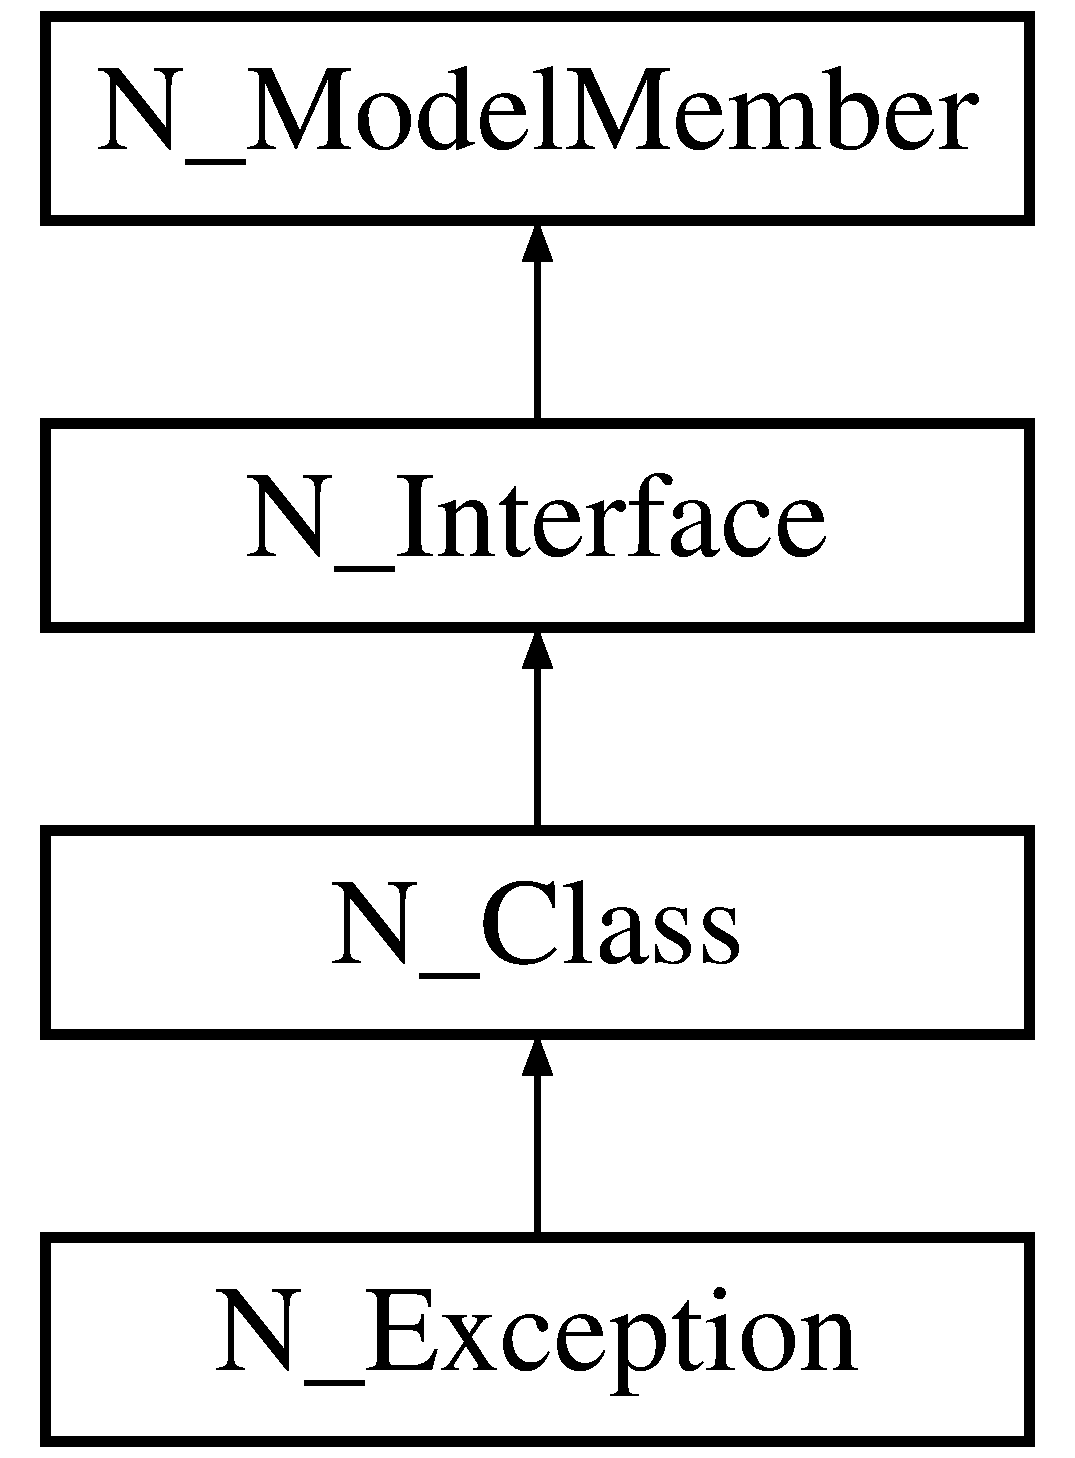
\includegraphics[height=4.000000cm]{classN__Class}
\end{center}
\end{figure}
\subsection*{Public Member Functions}
\begin{DoxyCompactItemize}
\item 
\hyperlink{classN__Class_a3f3a1254f6370fcee748a50e460b0da4}{N\+\_\+\+Class} (std\+::string name)
\item 
virtual \hyperlink{classN__Class_a141071f7db3aba8a98af0e67d711d046}{$\sim$\+N\+\_\+\+Class} ()
\item 
virtual void \hyperlink{classN__Class_ae6be664192857da779ff575019321304}{add\+Field} (\hyperlink{classN__Field}{N\+\_\+\+Field} field)
\item 
virtual std\+::vector$<$ \hyperlink{classN__Field}{N\+\_\+\+Field} $>$ \hyperlink{classN__Class_a5caf6d52ac2fd564e1fa1c4a6b4e00f8}{get\+Fields} ()
\item 
virtual void \hyperlink{classN__Class_a2f6d7f3cbe120e4b38520fb1c95e4f42}{add\+Ancestor\+Class} (\hyperlink{classN__Class}{N\+\_\+\+Class} \&c)
\item 
virtual std\+::vector$<$ \hyperlink{classN__Class}{N\+\_\+\+Class} $>$ \hyperlink{classN__Class_aa27ad0ec290cf7dea9a479524e4b0192}{get\+Ancestor\+Classes} ()
\end{DoxyCompactItemize}
\subsection*{Protected Attributes}
\begin{DoxyCompactItemize}
\item 
std\+::vector$<$ \hyperlink{classN__Field}{N\+\_\+\+Field} $>$ \hyperlink{classN__Class_acafc087764ee9469711513ff7abc132f}{m\+\_\+fields}
\begin{DoxyCompactList}\small\item\em Коллекция полей класса \end{DoxyCompactList}\item 
std\+::vector$<$ \hyperlink{classN__Class}{N\+\_\+\+Class} $>$ \hyperlink{classN__Class_a643715744802bdaf7dd9fc4712036703}{m\+\_\+ancestor\+\_\+classes}
\begin{DoxyCompactList}\small\item\em Коллекция классов-\/предков \end{DoxyCompactList}\end{DoxyCompactItemize}


\subsection{Detailed Description}
Нетерминал, обозначающий класс. 

\subsection{Constructor \& Destructor Documentation}
\hypertarget{classN__Class_a3f3a1254f6370fcee748a50e460b0da4}{}\index{N\+\_\+\+Class@{N\+\_\+\+Class}!N\+\_\+\+Class@{N\+\_\+\+Class}}
\index{N\+\_\+\+Class@{N\+\_\+\+Class}!N\+\_\+\+Class@{N\+\_\+\+Class}}
\subsubsection[{N\+\_\+\+Class}]{\setlength{\rightskip}{0pt plus 5cm}N\+\_\+\+Class\+::\+N\+\_\+\+Class (
\begin{DoxyParamCaption}
\item[{std\+::string}]{name}
\end{DoxyParamCaption}
)\hspace{0.3cm}{\ttfamily [inline]}}\label{classN__Class_a3f3a1254f6370fcee748a50e460b0da4}
Конструктор 
\begin{DoxyParams}{Parameters}
{\em name} & -\/ имя класса \\
\hline
\end{DoxyParams}
\hypertarget{classN__Class_a141071f7db3aba8a98af0e67d711d046}{}\index{N\+\_\+\+Class@{N\+\_\+\+Class}!````~N\+\_\+\+Class@{$\sim$\+N\+\_\+\+Class}}
\index{````~N\+\_\+\+Class@{$\sim$\+N\+\_\+\+Class}!N\+\_\+\+Class@{N\+\_\+\+Class}}
\subsubsection[{$\sim$\+N\+\_\+\+Class}]{\setlength{\rightskip}{0pt plus 5cm}virtual N\+\_\+\+Class\+::$\sim$\+N\+\_\+\+Class (
\begin{DoxyParamCaption}
{}
\end{DoxyParamCaption}
)\hspace{0.3cm}{\ttfamily [inline]}, {\ttfamily [virtual]}}\label{classN__Class_a141071f7db3aba8a98af0e67d711d046}
Деструктор 

\subsection{Member Function Documentation}
\hypertarget{classN__Class_a2f6d7f3cbe120e4b38520fb1c95e4f42}{}\index{N\+\_\+\+Class@{N\+\_\+\+Class}!add\+Ancestor\+Class@{add\+Ancestor\+Class}}
\index{add\+Ancestor\+Class@{add\+Ancestor\+Class}!N\+\_\+\+Class@{N\+\_\+\+Class}}
\subsubsection[{add\+Ancestor\+Class}]{\setlength{\rightskip}{0pt plus 5cm}virtual void N\+\_\+\+Class\+::add\+Ancestor\+Class (
\begin{DoxyParamCaption}
\item[{{\bf N\+\_\+\+Class} \&}]{c}
\end{DoxyParamCaption}
)\hspace{0.3cm}{\ttfamily [inline]}, {\ttfamily [virtual]}}\label{classN__Class_a2f6d7f3cbe120e4b38520fb1c95e4f42}
Добавление класса-\/предка 
\begin{DoxyParams}{Parameters}
{\em c} & -\/ класс, который необходимо добавить в качестве предка \\
\hline
\end{DoxyParams}
\hypertarget{classN__Class_ae6be664192857da779ff575019321304}{}\index{N\+\_\+\+Class@{N\+\_\+\+Class}!add\+Field@{add\+Field}}
\index{add\+Field@{add\+Field}!N\+\_\+\+Class@{N\+\_\+\+Class}}
\subsubsection[{add\+Field}]{\setlength{\rightskip}{0pt plus 5cm}virtual void N\+\_\+\+Class\+::add\+Field (
\begin{DoxyParamCaption}
\item[{{\bf N\+\_\+\+Field}}]{field}
\end{DoxyParamCaption}
)\hspace{0.3cm}{\ttfamily [inline]}, {\ttfamily [virtual]}}\label{classN__Class_ae6be664192857da779ff575019321304}
Добавление поля в класс 
\begin{DoxyParams}{Parameters}
{\em field} & -\/ поле, которе необходимо добавить в класс \\
\hline
\end{DoxyParams}
\hypertarget{classN__Class_aa27ad0ec290cf7dea9a479524e4b0192}{}\index{N\+\_\+\+Class@{N\+\_\+\+Class}!get\+Ancestor\+Classes@{get\+Ancestor\+Classes}}
\index{get\+Ancestor\+Classes@{get\+Ancestor\+Classes}!N\+\_\+\+Class@{N\+\_\+\+Class}}
\subsubsection[{get\+Ancestor\+Classes}]{\setlength{\rightskip}{0pt plus 5cm}virtual std\+::vector$<${\bf N\+\_\+\+Class}$>$ N\+\_\+\+Class\+::get\+Ancestor\+Classes (
\begin{DoxyParamCaption}
{}
\end{DoxyParamCaption}
)\hspace{0.3cm}{\ttfamily [inline]}, {\ttfamily [virtual]}}\label{classN__Class_aa27ad0ec290cf7dea9a479524e4b0192}
Получение коллекции классов-\/предков \begin{DoxyReturn}{Returns}
Коллекция классов-\/предков 
\end{DoxyReturn}
\hypertarget{classN__Class_a5caf6d52ac2fd564e1fa1c4a6b4e00f8}{}\index{N\+\_\+\+Class@{N\+\_\+\+Class}!get\+Fields@{get\+Fields}}
\index{get\+Fields@{get\+Fields}!N\+\_\+\+Class@{N\+\_\+\+Class}}
\subsubsection[{get\+Fields}]{\setlength{\rightskip}{0pt plus 5cm}virtual std\+::vector$<${\bf N\+\_\+\+Field}$>$ N\+\_\+\+Class\+::get\+Fields (
\begin{DoxyParamCaption}
{}
\end{DoxyParamCaption}
)\hspace{0.3cm}{\ttfamily [inline]}, {\ttfamily [virtual]}}\label{classN__Class_a5caf6d52ac2fd564e1fa1c4a6b4e00f8}
Получение коллекции полей класса \begin{DoxyReturn}{Returns}
Коллекция полей класса 
\end{DoxyReturn}


\subsection{Member Data Documentation}
\hypertarget{classN__Class_a643715744802bdaf7dd9fc4712036703}{}\index{N\+\_\+\+Class@{N\+\_\+\+Class}!m\+\_\+ancestor\+\_\+classes@{m\+\_\+ancestor\+\_\+classes}}
\index{m\+\_\+ancestor\+\_\+classes@{m\+\_\+ancestor\+\_\+classes}!N\+\_\+\+Class@{N\+\_\+\+Class}}
\subsubsection[{m\+\_\+ancestor\+\_\+classes}]{\setlength{\rightskip}{0pt plus 5cm}std\+::vector$<${\bf N\+\_\+\+Class}$>$ N\+\_\+\+Class\+::m\+\_\+ancestor\+\_\+classes\hspace{0.3cm}{\ttfamily [protected]}}\label{classN__Class_a643715744802bdaf7dd9fc4712036703}


Коллекция классов-\/предков 

\hypertarget{classN__Class_acafc087764ee9469711513ff7abc132f}{}\index{N\+\_\+\+Class@{N\+\_\+\+Class}!m\+\_\+fields@{m\+\_\+fields}}
\index{m\+\_\+fields@{m\+\_\+fields}!N\+\_\+\+Class@{N\+\_\+\+Class}}
\subsubsection[{m\+\_\+fields}]{\setlength{\rightskip}{0pt plus 5cm}std\+::vector$<${\bf N\+\_\+\+Field}$>$ N\+\_\+\+Class\+::m\+\_\+fields\hspace{0.3cm}{\ttfamily [protected]}}\label{classN__Class_acafc087764ee9469711513ff7abc132f}


Коллекция полей класса 



The documentation for this class was generated from the following file\+:\begin{DoxyCompactItemize}
\item 
\hyperlink{ast_8h}{ast.\+h}\end{DoxyCompactItemize}

\hypertarget{classN__ClassMember}{}\section{N\+\_\+\+Class\+Member Class Reference}
\label{classN__ClassMember}\index{N\+\_\+\+Class\+Member@{N\+\_\+\+Class\+Member}}


{\ttfamily \#include $<$ast.\+h$>$}

Inheritance diagram for N\+\_\+\+Class\+Member\+:\begin{figure}[H]
\begin{center}
\leavevmode
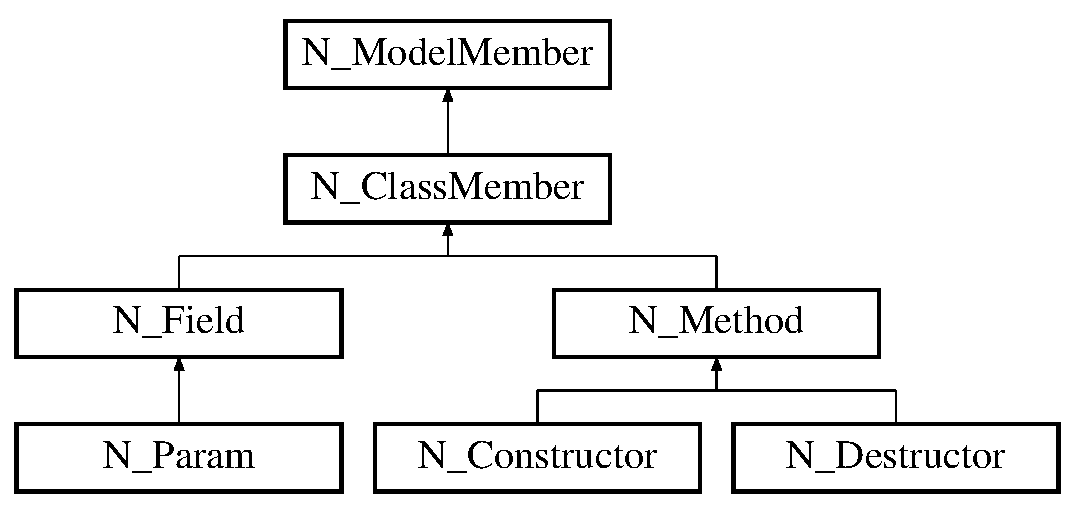
\includegraphics[height=4.000000cm]{classN__ClassMember}
\end{center}
\end{figure}
\subsection*{Public Member Functions}
\begin{DoxyCompactItemize}
\item 
\hyperlink{classN__ClassMember_a579c8df412a16010bb152661ce8b07c9}{N\+\_\+\+Class\+Member} (const std\+::string \&name, const std\+::string \&type, \hyperlink{ast_8h_a8cf536792064de0e4fc620bc6f1dc90e}{Member\+Visibility} vis=\hyperlink{ast_8h_a8cf536792064de0e4fc620bc6f1dc90eae560d950ff759756c70399d8cfe015d0}{M\+V\+\_\+\+P\+R\+I\+V\+A\+T\+E})
\item 
virtual \hyperlink{classN__ClassMember_a7f5c3fa0c8df7ce0578a64a3ec6014df}{$\sim$\+N\+\_\+\+Class\+Member} ()
\item 
virtual \hyperlink{classN__Type}{N\+\_\+\+Type} \& \hyperlink{classN__ClassMember_a40afd3c10cbd60a14b88f5b615be79d6}{get\+Type} ()
\item 
virtual \hyperlink{ast_8h_a8cf536792064de0e4fc620bc6f1dc90e}{Member\+Visibility} \hyperlink{classN__ClassMember_a9d497fb4fd82c625095f8e8e7d60905d}{get\+Visibility} () const 
\item 
virtual void \hyperlink{classN__ClassMember_a859513b443ae1cd658241eca4be8b604}{set\+Static} (bool st)
\item 
virtual bool \hyperlink{classN__ClassMember_af26e06acc9e1eaacbccdfb0bced394d2}{is\+Static} () const 
\end{DoxyCompactItemize}
\subsection*{Protected Attributes}
\begin{DoxyCompactItemize}
\item 
\hyperlink{classN__Type}{N\+\_\+\+Type} \hyperlink{classN__ClassMember_a0a5a7b177d59cad12e472cfc13663bba}{m\+\_\+type}
\begin{DoxyCompactList}\small\item\em Тип члена класса \end{DoxyCompactList}\item 
\hyperlink{ast_8h_a8cf536792064de0e4fc620bc6f1dc90e}{Member\+Visibility} \hyperlink{classN__ClassMember_ac035d5da0f01fc5323eb9fb3dfdd5bf5}{m\+\_\+vis}
\begin{DoxyCompactList}\small\item\em Область видимости члена класса \end{DoxyCompactList}\item 
bool \hyperlink{classN__ClassMember_a3149a9790156445d10c9774976890e92}{m\+\_\+static}
\begin{DoxyCompactList}\small\item\em Является ли член класса статическим \end{DoxyCompactList}\end{DoxyCompactItemize}


\subsection{Detailed Description}
Член класса 

\subsection{Constructor \& Destructor Documentation}
\hypertarget{classN__ClassMember_a579c8df412a16010bb152661ce8b07c9}{}\index{N\+\_\+\+Class\+Member@{N\+\_\+\+Class\+Member}!N\+\_\+\+Class\+Member@{N\+\_\+\+Class\+Member}}
\index{N\+\_\+\+Class\+Member@{N\+\_\+\+Class\+Member}!N\+\_\+\+Class\+Member@{N\+\_\+\+Class\+Member}}
\subsubsection[{N\+\_\+\+Class\+Member}]{\setlength{\rightskip}{0pt plus 5cm}N\+\_\+\+Class\+Member\+::\+N\+\_\+\+Class\+Member (
\begin{DoxyParamCaption}
\item[{const std\+::string \&}]{name, }
\item[{const std\+::string \&}]{type, }
\item[{{\bf Member\+Visibility}}]{vis = {\ttfamily {\bf M\+V\+\_\+\+P\+R\+I\+V\+A\+T\+E}}}
\end{DoxyParamCaption}
)\hspace{0.3cm}{\ttfamily [inline]}}\label{classN__ClassMember_a579c8df412a16010bb152661ce8b07c9}
Конструктор 
\begin{DoxyParams}{Parameters}
{\em name} & -\/ имя члена класса \\
\hline
{\em type} & -\/ тип члена класса \\
\hline
{\em vis} & -\/ область видимости члена класса \\
\hline
\end{DoxyParams}
\hypertarget{classN__ClassMember_a7f5c3fa0c8df7ce0578a64a3ec6014df}{}\index{N\+\_\+\+Class\+Member@{N\+\_\+\+Class\+Member}!````~N\+\_\+\+Class\+Member@{$\sim$\+N\+\_\+\+Class\+Member}}
\index{````~N\+\_\+\+Class\+Member@{$\sim$\+N\+\_\+\+Class\+Member}!N\+\_\+\+Class\+Member@{N\+\_\+\+Class\+Member}}
\subsubsection[{$\sim$\+N\+\_\+\+Class\+Member}]{\setlength{\rightskip}{0pt plus 5cm}virtual N\+\_\+\+Class\+Member\+::$\sim$\+N\+\_\+\+Class\+Member (
\begin{DoxyParamCaption}
{}
\end{DoxyParamCaption}
)\hspace{0.3cm}{\ttfamily [inline]}, {\ttfamily [virtual]}}\label{classN__ClassMember_a7f5c3fa0c8df7ce0578a64a3ec6014df}
Деструктор 

\subsection{Member Function Documentation}
\hypertarget{classN__ClassMember_a40afd3c10cbd60a14b88f5b615be79d6}{}\index{N\+\_\+\+Class\+Member@{N\+\_\+\+Class\+Member}!get\+Type@{get\+Type}}
\index{get\+Type@{get\+Type}!N\+\_\+\+Class\+Member@{N\+\_\+\+Class\+Member}}
\subsubsection[{get\+Type}]{\setlength{\rightskip}{0pt plus 5cm}virtual {\bf N\+\_\+\+Type}\& N\+\_\+\+Class\+Member\+::get\+Type (
\begin{DoxyParamCaption}
{}
\end{DoxyParamCaption}
)\hspace{0.3cm}{\ttfamily [inline]}, {\ttfamily [virtual]}}\label{classN__ClassMember_a40afd3c10cbd60a14b88f5b615be79d6}
Получение типа члена класса \begin{DoxyReturn}{Returns}
тип члена класса 
\end{DoxyReturn}
\hypertarget{classN__ClassMember_a9d497fb4fd82c625095f8e8e7d60905d}{}\index{N\+\_\+\+Class\+Member@{N\+\_\+\+Class\+Member}!get\+Visibility@{get\+Visibility}}
\index{get\+Visibility@{get\+Visibility}!N\+\_\+\+Class\+Member@{N\+\_\+\+Class\+Member}}
\subsubsection[{get\+Visibility}]{\setlength{\rightskip}{0pt plus 5cm}virtual {\bf Member\+Visibility} N\+\_\+\+Class\+Member\+::get\+Visibility (
\begin{DoxyParamCaption}
{}
\end{DoxyParamCaption}
) const\hspace{0.3cm}{\ttfamily [inline]}, {\ttfamily [virtual]}}\label{classN__ClassMember_a9d497fb4fd82c625095f8e8e7d60905d}
Получение области видимости члена класса \begin{DoxyReturn}{Returns}
область видимости члена класса 
\end{DoxyReturn}
\hypertarget{classN__ClassMember_af26e06acc9e1eaacbccdfb0bced394d2}{}\index{N\+\_\+\+Class\+Member@{N\+\_\+\+Class\+Member}!is\+Static@{is\+Static}}
\index{is\+Static@{is\+Static}!N\+\_\+\+Class\+Member@{N\+\_\+\+Class\+Member}}
\subsubsection[{is\+Static}]{\setlength{\rightskip}{0pt plus 5cm}virtual bool N\+\_\+\+Class\+Member\+::is\+Static (
\begin{DoxyParamCaption}
{}
\end{DoxyParamCaption}
) const\hspace{0.3cm}{\ttfamily [inline]}, {\ttfamily [virtual]}}\label{classN__ClassMember_af26e06acc9e1eaacbccdfb0bced394d2}
Получение признака статического члена класса \begin{DoxyReturn}{Returns}
значение признака 
\end{DoxyReturn}
\hypertarget{classN__ClassMember_a859513b443ae1cd658241eca4be8b604}{}\index{N\+\_\+\+Class\+Member@{N\+\_\+\+Class\+Member}!set\+Static@{set\+Static}}
\index{set\+Static@{set\+Static}!N\+\_\+\+Class\+Member@{N\+\_\+\+Class\+Member}}
\subsubsection[{set\+Static}]{\setlength{\rightskip}{0pt plus 5cm}virtual void N\+\_\+\+Class\+Member\+::set\+Static (
\begin{DoxyParamCaption}
\item[{bool}]{st}
\end{DoxyParamCaption}
)\hspace{0.3cm}{\ttfamily [inline]}, {\ttfamily [virtual]}}\label{classN__ClassMember_a859513b443ae1cd658241eca4be8b604}
Установка признака статического члена класса 
\begin{DoxyParams}{Parameters}
{\em st} & -\/ значение признака \\
\hline
\end{DoxyParams}


\subsection{Member Data Documentation}
\hypertarget{classN__ClassMember_a3149a9790156445d10c9774976890e92}{}\index{N\+\_\+\+Class\+Member@{N\+\_\+\+Class\+Member}!m\+\_\+static@{m\+\_\+static}}
\index{m\+\_\+static@{m\+\_\+static}!N\+\_\+\+Class\+Member@{N\+\_\+\+Class\+Member}}
\subsubsection[{m\+\_\+static}]{\setlength{\rightskip}{0pt plus 5cm}bool N\+\_\+\+Class\+Member\+::m\+\_\+static\hspace{0.3cm}{\ttfamily [protected]}}\label{classN__ClassMember_a3149a9790156445d10c9774976890e92}


Является ли член класса статическим 

\hypertarget{classN__ClassMember_a0a5a7b177d59cad12e472cfc13663bba}{}\index{N\+\_\+\+Class\+Member@{N\+\_\+\+Class\+Member}!m\+\_\+type@{m\+\_\+type}}
\index{m\+\_\+type@{m\+\_\+type}!N\+\_\+\+Class\+Member@{N\+\_\+\+Class\+Member}}
\subsubsection[{m\+\_\+type}]{\setlength{\rightskip}{0pt plus 5cm}{\bf N\+\_\+\+Type} N\+\_\+\+Class\+Member\+::m\+\_\+type\hspace{0.3cm}{\ttfamily [protected]}}\label{classN__ClassMember_a0a5a7b177d59cad12e472cfc13663bba}


Тип члена класса 

\hypertarget{classN__ClassMember_ac035d5da0f01fc5323eb9fb3dfdd5bf5}{}\index{N\+\_\+\+Class\+Member@{N\+\_\+\+Class\+Member}!m\+\_\+vis@{m\+\_\+vis}}
\index{m\+\_\+vis@{m\+\_\+vis}!N\+\_\+\+Class\+Member@{N\+\_\+\+Class\+Member}}
\subsubsection[{m\+\_\+vis}]{\setlength{\rightskip}{0pt plus 5cm}{\bf Member\+Visibility} N\+\_\+\+Class\+Member\+::m\+\_\+vis\hspace{0.3cm}{\ttfamily [protected]}}\label{classN__ClassMember_ac035d5da0f01fc5323eb9fb3dfdd5bf5}


Область видимости члена класса 



The documentation for this class was generated from the following file\+:\begin{DoxyCompactItemize}
\item 
\hyperlink{ast_8h}{ast.\+h}\end{DoxyCompactItemize}

\hypertarget{classN__Constructor}{}\section{N\+\_\+\+Constructor Class Reference}
\label{classN__Constructor}\index{N\+\_\+\+Constructor@{N\+\_\+\+Constructor}}


{\ttfamily \#include $<$ast.\+h$>$}

Inheritance diagram for N\+\_\+\+Constructor\+:\begin{figure}[H]
\begin{center}
\leavevmode
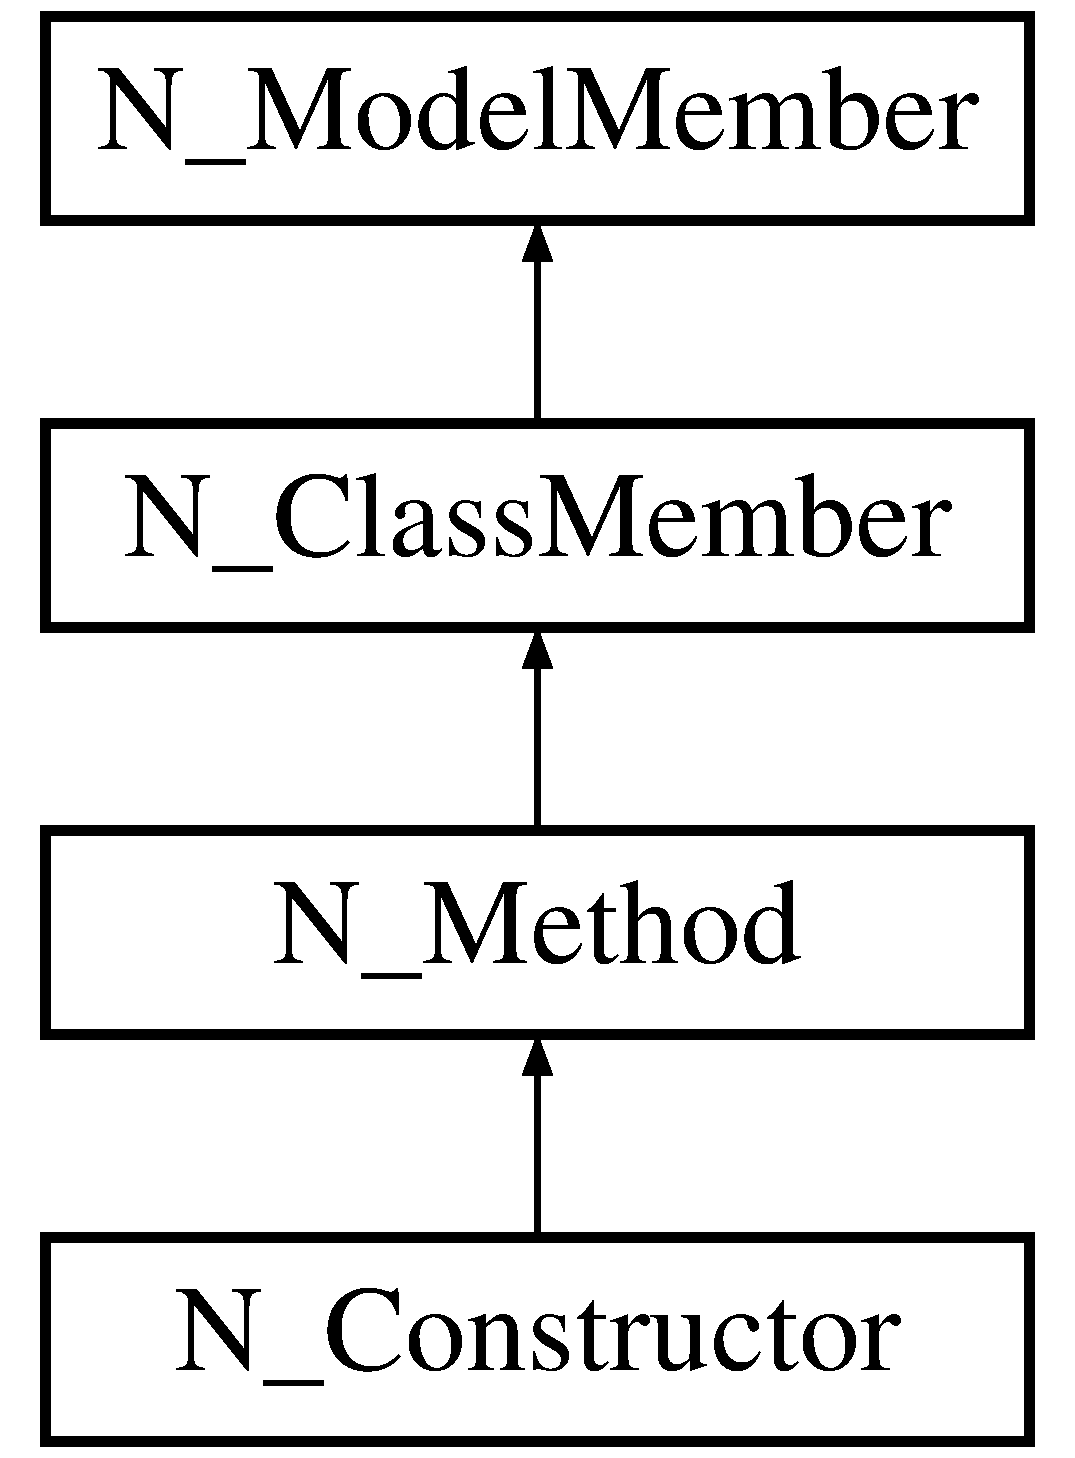
\includegraphics[height=4.000000cm]{classN__Constructor}
\end{center}
\end{figure}
\subsection*{Public Member Functions}
\begin{DoxyCompactItemize}
\item 
\hyperlink{classN__Constructor_a24df433dc9052a31abb4672dbee60db3}{N\+\_\+\+Constructor} (const std\+::string \&name, \hyperlink{ast_8h_a8cf536792064de0e4fc620bc6f1dc90e}{Member\+Visibility} vis=\hyperlink{ast_8h_a8cf536792064de0e4fc620bc6f1dc90eae560d950ff759756c70399d8cfe015d0}{M\+V\+\_\+\+P\+R\+I\+V\+A\+T\+E})
\item 
virtual \hyperlink{classN__Constructor_a9992d88e196d85dbb3658c3d522f5f8d}{$\sim$\+N\+\_\+\+Constructor} ()
\end{DoxyCompactItemize}
\subsection*{Additional Inherited Members}


\subsection{Detailed Description}
Нетерминал, обозначающий конструктор 

\subsection{Constructor \& Destructor Documentation}
\hypertarget{classN__Constructor_a24df433dc9052a31abb4672dbee60db3}{}\index{N\+\_\+\+Constructor@{N\+\_\+\+Constructor}!N\+\_\+\+Constructor@{N\+\_\+\+Constructor}}
\index{N\+\_\+\+Constructor@{N\+\_\+\+Constructor}!N\+\_\+\+Constructor@{N\+\_\+\+Constructor}}
\subsubsection[{N\+\_\+\+Constructor}]{\setlength{\rightskip}{0pt plus 5cm}N\+\_\+\+Constructor\+::\+N\+\_\+\+Constructor (
\begin{DoxyParamCaption}
\item[{const std\+::string \&}]{name, }
\item[{{\bf Member\+Visibility}}]{vis = {\ttfamily {\bf M\+V\+\_\+\+P\+R\+I\+V\+A\+T\+E}}}
\end{DoxyParamCaption}
)\hspace{0.3cm}{\ttfamily [inline]}}\label{classN__Constructor_a24df433dc9052a31abb4672dbee60db3}
Конструктор 
\begin{DoxyParams}{Parameters}
{\em name} & -\/ имя конструктора (если применимо) \\
\hline
{\em vis} & -\/ область видимости конструктора \\
\hline
\end{DoxyParams}
\hypertarget{classN__Constructor_a9992d88e196d85dbb3658c3d522f5f8d}{}\index{N\+\_\+\+Constructor@{N\+\_\+\+Constructor}!````~N\+\_\+\+Constructor@{$\sim$\+N\+\_\+\+Constructor}}
\index{````~N\+\_\+\+Constructor@{$\sim$\+N\+\_\+\+Constructor}!N\+\_\+\+Constructor@{N\+\_\+\+Constructor}}
\subsubsection[{$\sim$\+N\+\_\+\+Constructor}]{\setlength{\rightskip}{0pt plus 5cm}virtual N\+\_\+\+Constructor\+::$\sim$\+N\+\_\+\+Constructor (
\begin{DoxyParamCaption}
{}
\end{DoxyParamCaption}
)\hspace{0.3cm}{\ttfamily [inline]}, {\ttfamily [virtual]}}\label{classN__Constructor_a9992d88e196d85dbb3658c3d522f5f8d}
Деструктор 

The documentation for this class was generated from the following file\+:\begin{DoxyCompactItemize}
\item 
\hyperlink{ast_8h}{ast.\+h}\end{DoxyCompactItemize}

\hypertarget{classN__Destructor}{}\section{N\+\_\+\+Destructor Class Reference}
\label{classN__Destructor}\index{N\+\_\+\+Destructor@{N\+\_\+\+Destructor}}


{\ttfamily \#include $<$ast.\+h$>$}

Inheritance diagram for N\+\_\+\+Destructor\+:\begin{figure}[H]
\begin{center}
\leavevmode
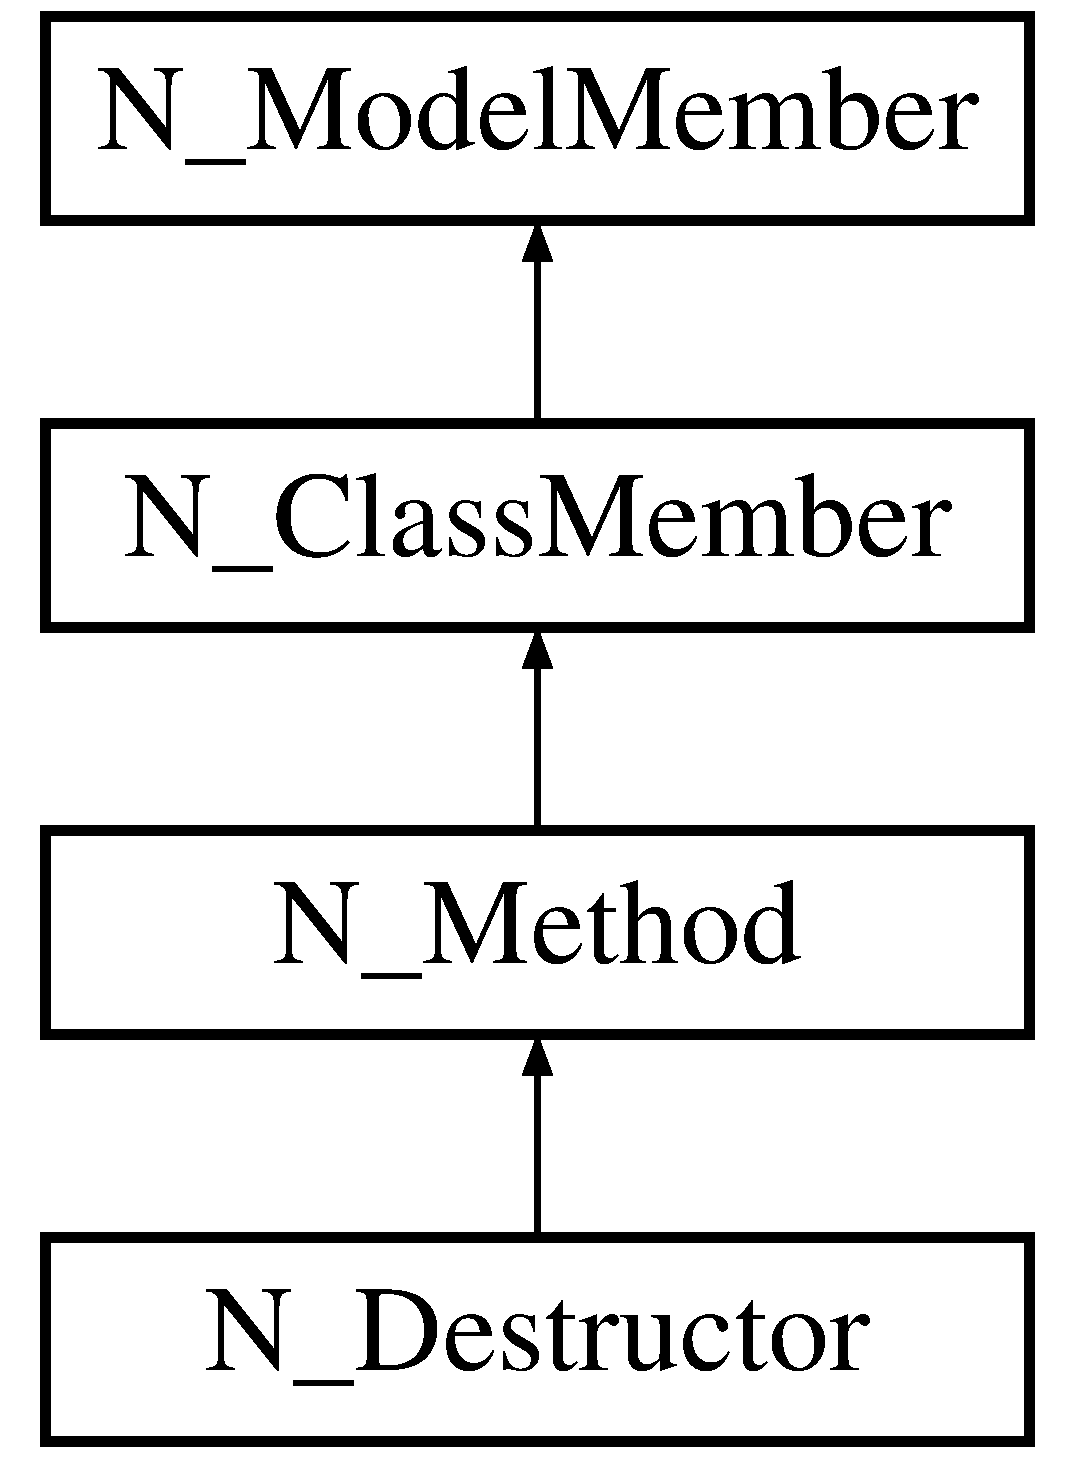
\includegraphics[height=4.000000cm]{classN__Destructor}
\end{center}
\end{figure}
\subsection*{Public Member Functions}
\begin{DoxyCompactItemize}
\item 
\hyperlink{classN__Destructor_aa57bd73ddebd0cf0ff3f28a7fb0fabd0}{N\+\_\+\+Destructor} (const std\+::string \&name, \hyperlink{ast_8h_a8cf536792064de0e4fc620bc6f1dc90e}{Member\+Visibility} vis=\hyperlink{ast_8h_a8cf536792064de0e4fc620bc6f1dc90eae560d950ff759756c70399d8cfe015d0}{M\+V\+\_\+\+P\+R\+I\+V\+A\+T\+E})
\item 
virtual \hyperlink{classN__Destructor_a6575c6a0505d9ffa3efdaaa9c150d4a3}{$\sim$\+N\+\_\+\+Destructor} ()
\end{DoxyCompactItemize}
\subsection*{Additional Inherited Members}


\subsection{Detailed Description}
Нетерминал, обозначающий деструктор 

\subsection{Constructor \& Destructor Documentation}
\hypertarget{classN__Destructor_aa57bd73ddebd0cf0ff3f28a7fb0fabd0}{}\index{N\+\_\+\+Destructor@{N\+\_\+\+Destructor}!N\+\_\+\+Destructor@{N\+\_\+\+Destructor}}
\index{N\+\_\+\+Destructor@{N\+\_\+\+Destructor}!N\+\_\+\+Destructor@{N\+\_\+\+Destructor}}
\subsubsection[{N\+\_\+\+Destructor}]{\setlength{\rightskip}{0pt plus 5cm}N\+\_\+\+Destructor\+::\+N\+\_\+\+Destructor (
\begin{DoxyParamCaption}
\item[{const std\+::string \&}]{name, }
\item[{{\bf Member\+Visibility}}]{vis = {\ttfamily {\bf M\+V\+\_\+\+P\+R\+I\+V\+A\+T\+E}}}
\end{DoxyParamCaption}
)\hspace{0.3cm}{\ttfamily [inline]}}\label{classN__Destructor_aa57bd73ddebd0cf0ff3f28a7fb0fabd0}
Конструктор 
\begin{DoxyParams}{Parameters}
{\em name} & -\/ имя деструктора (если применимо) \\
\hline
{\em vis} & -\/ область видимость деструктора \\
\hline
\end{DoxyParams}
\hypertarget{classN__Destructor_a6575c6a0505d9ffa3efdaaa9c150d4a3}{}\index{N\+\_\+\+Destructor@{N\+\_\+\+Destructor}!````~N\+\_\+\+Destructor@{$\sim$\+N\+\_\+\+Destructor}}
\index{````~N\+\_\+\+Destructor@{$\sim$\+N\+\_\+\+Destructor}!N\+\_\+\+Destructor@{N\+\_\+\+Destructor}}
\subsubsection[{$\sim$\+N\+\_\+\+Destructor}]{\setlength{\rightskip}{0pt plus 5cm}virtual N\+\_\+\+Destructor\+::$\sim$\+N\+\_\+\+Destructor (
\begin{DoxyParamCaption}
{}
\end{DoxyParamCaption}
)\hspace{0.3cm}{\ttfamily [inline]}, {\ttfamily [virtual]}}\label{classN__Destructor_a6575c6a0505d9ffa3efdaaa9c150d4a3}
Деструктор 

The documentation for this class was generated from the following file\+:\begin{DoxyCompactItemize}
\item 
\hyperlink{ast_8h}{ast.\+h}\end{DoxyCompactItemize}

\hypertarget{classN__Exception}{}\section{N\+\_\+\+Exception Class Reference}
\label{classN__Exception}\index{N\+\_\+\+Exception@{N\+\_\+\+Exception}}


{\ttfamily \#include $<$ast.\+h$>$}

Inheritance diagram for N\+\_\+\+Exception\+:\begin{figure}[H]
\begin{center}
\leavevmode
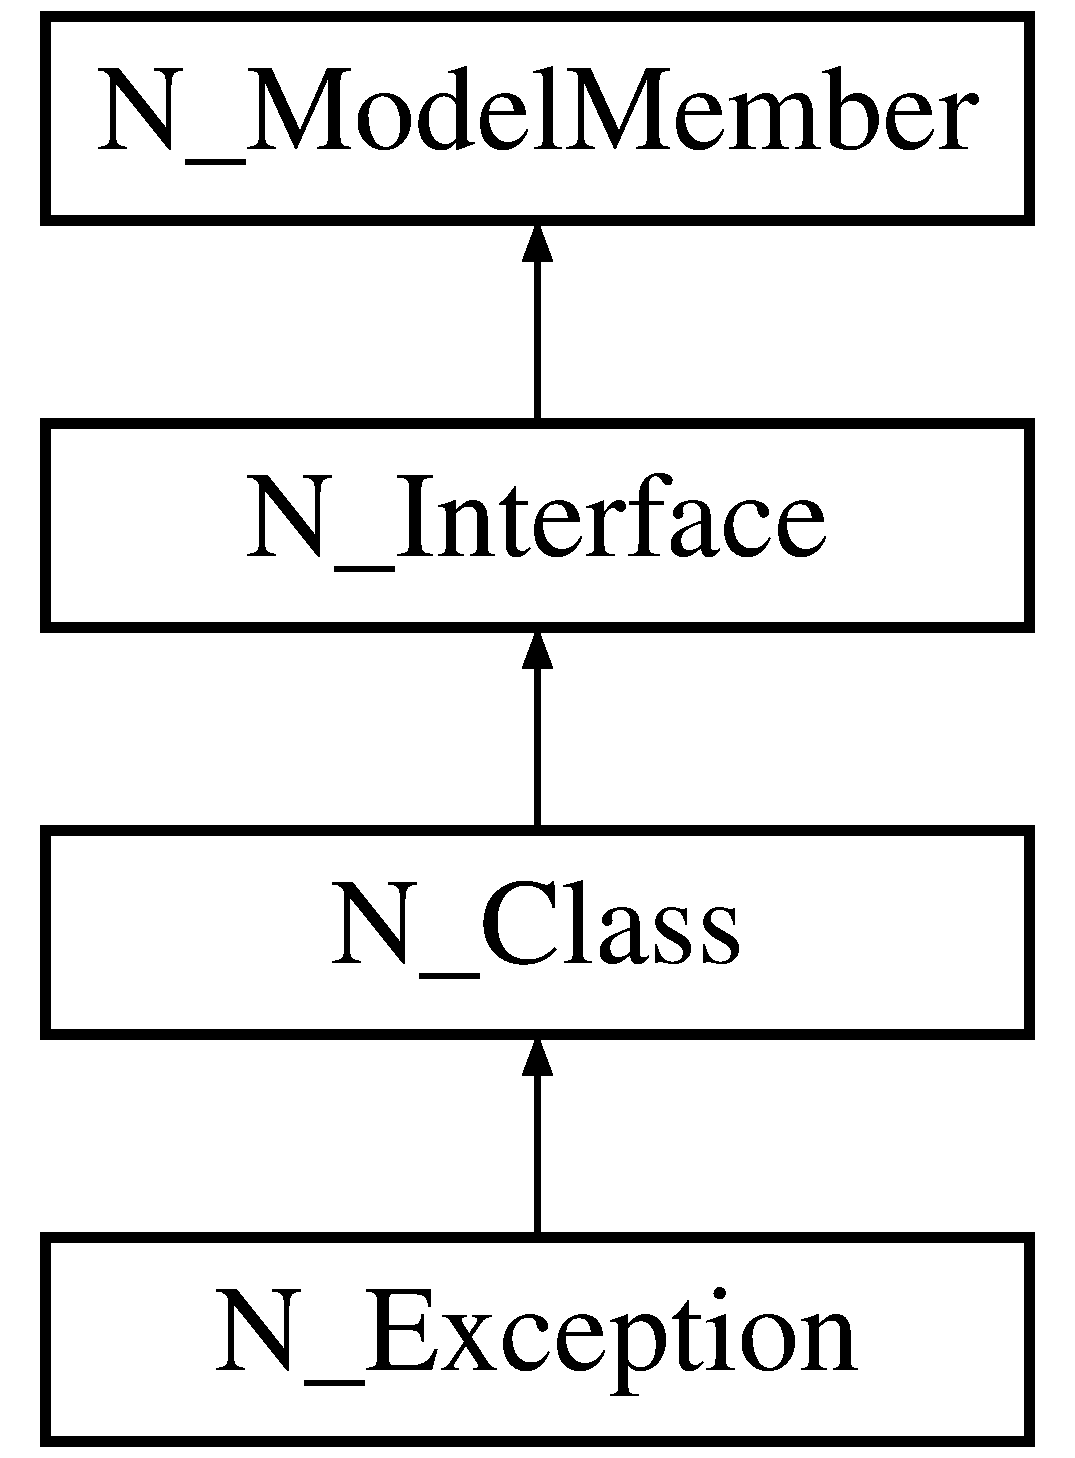
\includegraphics[height=4.000000cm]{classN__Exception}
\end{center}
\end{figure}
\subsection*{Public Member Functions}
\begin{DoxyCompactItemize}
\item 
\hyperlink{classN__Exception_ad705909149371a006ea58a28cb4aae24}{N\+\_\+\+Exception} (std\+::string name)
\item 
virtual \hyperlink{classN__Exception_aa30734467c1f14824e646aa7a69ea945}{$\sim$\+N\+\_\+\+Exception} ()
\end{DoxyCompactItemize}
\subsection*{Additional Inherited Members}


\subsection{Detailed Description}
Нетерминал, обозначающий класс-\/исключение 

\subsection{Constructor \& Destructor Documentation}
\hypertarget{classN__Exception_ad705909149371a006ea58a28cb4aae24}{}\index{N\+\_\+\+Exception@{N\+\_\+\+Exception}!N\+\_\+\+Exception@{N\+\_\+\+Exception}}
\index{N\+\_\+\+Exception@{N\+\_\+\+Exception}!N\+\_\+\+Exception@{N\+\_\+\+Exception}}
\subsubsection[{N\+\_\+\+Exception}]{\setlength{\rightskip}{0pt plus 5cm}N\+\_\+\+Exception\+::\+N\+\_\+\+Exception (
\begin{DoxyParamCaption}
\item[{std\+::string}]{name}
\end{DoxyParamCaption}
)\hspace{0.3cm}{\ttfamily [inline]}}\label{classN__Exception_ad705909149371a006ea58a28cb4aae24}
Конструктор 
\begin{DoxyParams}{Parameters}
{\em name} & -\/ имя исключения \\
\hline
\end{DoxyParams}
\hypertarget{classN__Exception_aa30734467c1f14824e646aa7a69ea945}{}\index{N\+\_\+\+Exception@{N\+\_\+\+Exception}!````~N\+\_\+\+Exception@{$\sim$\+N\+\_\+\+Exception}}
\index{````~N\+\_\+\+Exception@{$\sim$\+N\+\_\+\+Exception}!N\+\_\+\+Exception@{N\+\_\+\+Exception}}
\subsubsection[{$\sim$\+N\+\_\+\+Exception}]{\setlength{\rightskip}{0pt plus 5cm}virtual N\+\_\+\+Exception\+::$\sim$\+N\+\_\+\+Exception (
\begin{DoxyParamCaption}
{}
\end{DoxyParamCaption}
)\hspace{0.3cm}{\ttfamily [inline]}, {\ttfamily [virtual]}}\label{classN__Exception_aa30734467c1f14824e646aa7a69ea945}
Деструктор 

The documentation for this class was generated from the following file\+:\begin{DoxyCompactItemize}
\item 
\hyperlink{ast_8h}{ast.\+h}\end{DoxyCompactItemize}

\hypertarget{classN__Field}{}\section{N\+\_\+\+Field Class Reference}
\label{classN__Field}\index{N\+\_\+\+Field@{N\+\_\+\+Field}}


{\ttfamily \#include $<$ast.\+h$>$}

Inheritance diagram for N\+\_\+\+Field\+:\begin{figure}[H]
\begin{center}
\leavevmode
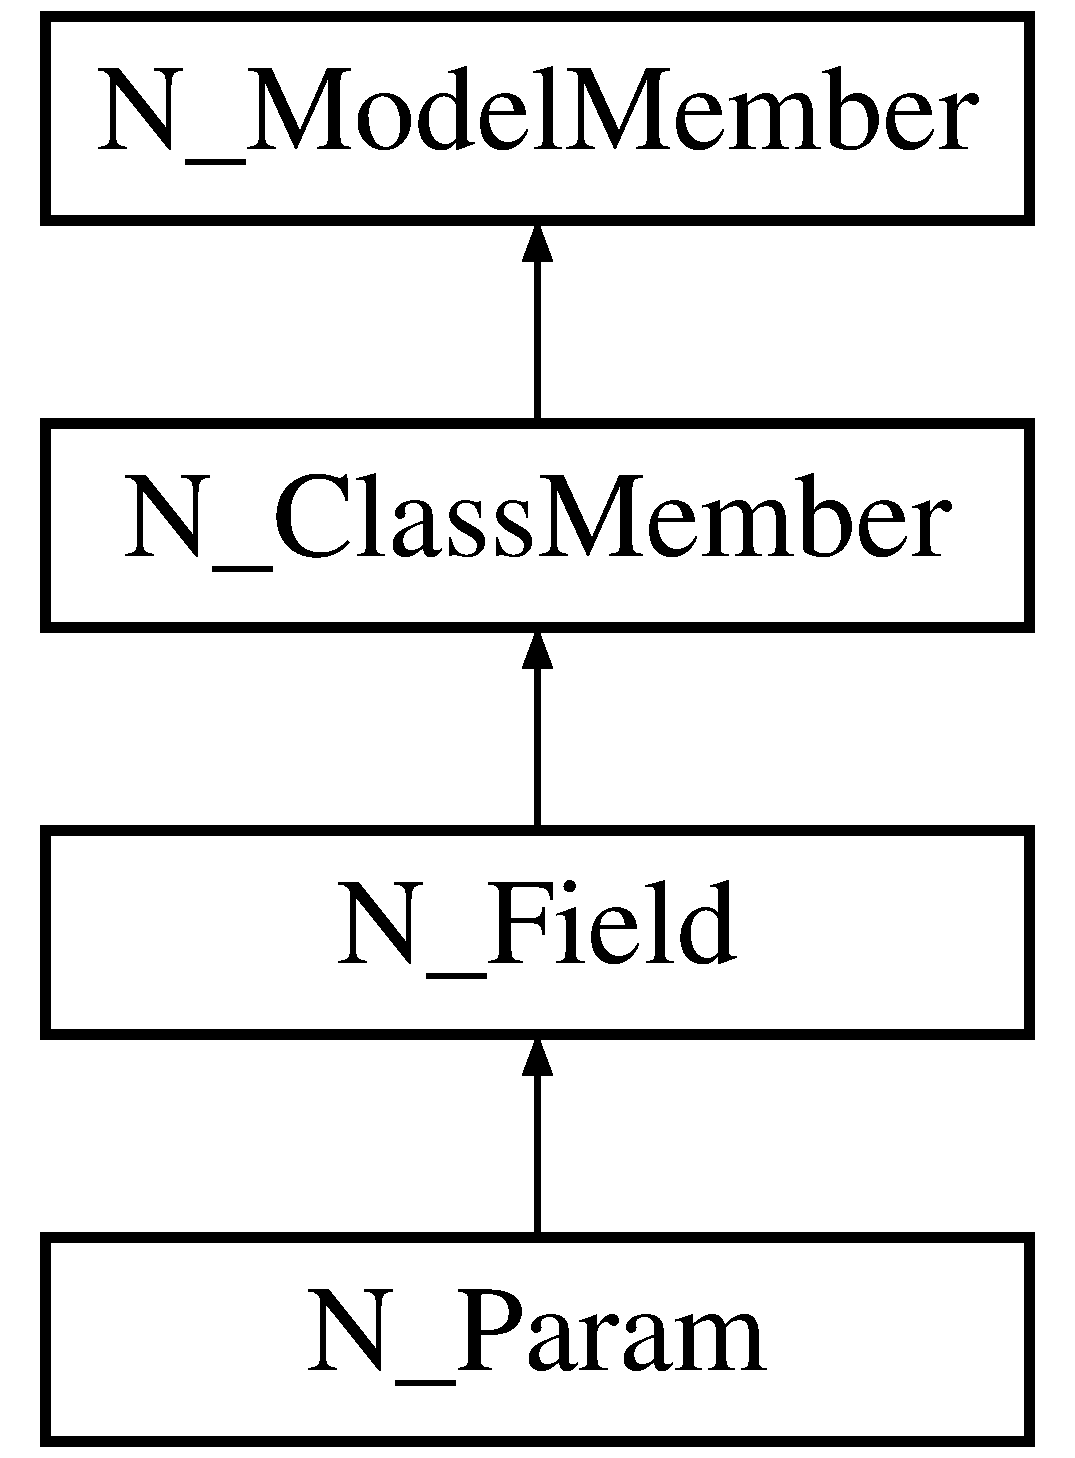
\includegraphics[height=4.000000cm]{classN__Field}
\end{center}
\end{figure}
\subsection*{Public Member Functions}
\begin{DoxyCompactItemize}
\item 
\hyperlink{classN__Field_a75e5ec7ff954a3529102a19c034977c6}{N\+\_\+\+Field} (const std\+::string \&name, const std\+::string \&type, \hyperlink{ast_8h_a8cf536792064de0e4fc620bc6f1dc90e}{Member\+Visibility} vis=\hyperlink{ast_8h_a8cf536792064de0e4fc620bc6f1dc90eae560d950ff759756c70399d8cfe015d0}{M\+V\+\_\+\+P\+R\+I\+V\+A\+T\+E})
\item 
virtual \hyperlink{classN__Field_af4633db19c3c931497cdc3ac98ff772b}{$\sim$\+N\+\_\+\+Field} ()
\end{DoxyCompactItemize}
\subsection*{Additional Inherited Members}


\subsection{Detailed Description}
Нетерминал, обозначающий поле класса 

\subsection{Constructor \& Destructor Documentation}
\hypertarget{classN__Field_a75e5ec7ff954a3529102a19c034977c6}{}\index{N\+\_\+\+Field@{N\+\_\+\+Field}!N\+\_\+\+Field@{N\+\_\+\+Field}}
\index{N\+\_\+\+Field@{N\+\_\+\+Field}!N\+\_\+\+Field@{N\+\_\+\+Field}}
\subsubsection[{N\+\_\+\+Field}]{\setlength{\rightskip}{0pt plus 5cm}N\+\_\+\+Field\+::\+N\+\_\+\+Field (
\begin{DoxyParamCaption}
\item[{const std\+::string \&}]{name, }
\item[{const std\+::string \&}]{type, }
\item[{{\bf Member\+Visibility}}]{vis = {\ttfamily {\bf M\+V\+\_\+\+P\+R\+I\+V\+A\+T\+E}}}
\end{DoxyParamCaption}
)\hspace{0.3cm}{\ttfamily [inline]}}\label{classN__Field_a75e5ec7ff954a3529102a19c034977c6}
Конструктор 
\begin{DoxyParams}{Parameters}
{\em name} & -\/ имя поля \\
\hline
{\em type} & -\/ тип поля \\
\hline
{\em vis} & -\/ область видимости поля \\
\hline
\end{DoxyParams}
\hypertarget{classN__Field_af4633db19c3c931497cdc3ac98ff772b}{}\index{N\+\_\+\+Field@{N\+\_\+\+Field}!````~N\+\_\+\+Field@{$\sim$\+N\+\_\+\+Field}}
\index{````~N\+\_\+\+Field@{$\sim$\+N\+\_\+\+Field}!N\+\_\+\+Field@{N\+\_\+\+Field}}
\subsubsection[{$\sim$\+N\+\_\+\+Field}]{\setlength{\rightskip}{0pt plus 5cm}virtual N\+\_\+\+Field\+::$\sim$\+N\+\_\+\+Field (
\begin{DoxyParamCaption}
{}
\end{DoxyParamCaption}
)\hspace{0.3cm}{\ttfamily [inline]}, {\ttfamily [virtual]}}\label{classN__Field_af4633db19c3c931497cdc3ac98ff772b}
Деструктор 

The documentation for this class was generated from the following file\+:\begin{DoxyCompactItemize}
\item 
\hyperlink{ast_8h}{ast.\+h}\end{DoxyCompactItemize}

\hypertarget{classN__Interface}{}\section{N\+\_\+\+Interface Class Reference}
\label{classN__Interface}\index{N\+\_\+\+Interface@{N\+\_\+\+Interface}}


{\ttfamily \#include $<$ast.\+h$>$}

Inheritance diagram for N\+\_\+\+Interface\+:\begin{figure}[H]
\begin{center}
\leavevmode
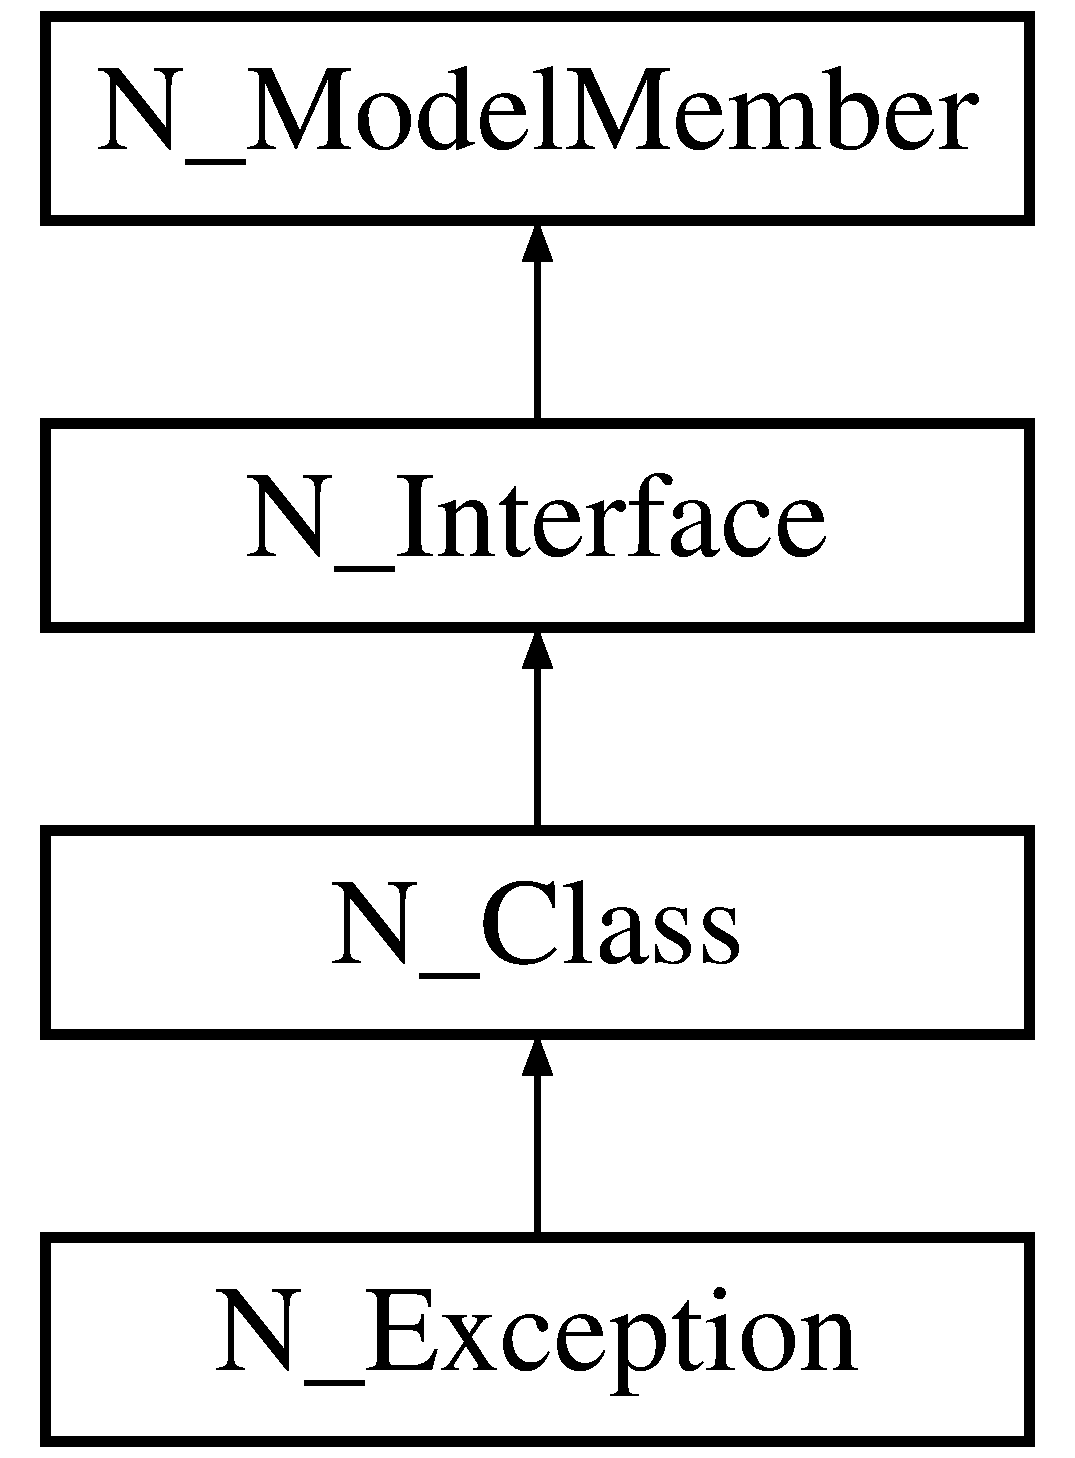
\includegraphics[height=4.000000cm]{classN__Interface}
\end{center}
\end{figure}
\subsection*{Public Member Functions}
\begin{DoxyCompactItemize}
\item 
\hyperlink{classN__Interface_a6127252915b959e78a3c47c21ddb54f4}{N\+\_\+\+Interface} (std\+::string name)
\item 
virtual \hyperlink{classN__Interface_a3f09f32cb660660a7b03331f31a8b904}{$\sim$\+N\+\_\+\+Interface} ()
\item 
virtual void \hyperlink{classN__Interface_a4beb006efe4088bf7b243fa93935b369}{add\+Method} (\hyperlink{classN__Method}{N\+\_\+\+Method} \&method)
\item 
virtual std\+::vector$<$ \hyperlink{classN__Method}{N\+\_\+\+Method} $>$ \hyperlink{classN__Interface_af17e8ba1285e33747c37b2517178215a}{get\+Methods} ()
\item 
virtual void \hyperlink{classN__Interface_a04397ba5bc93dd83a3b601faf79768e5}{add\+Ancestor\+Interface} (\hyperlink{classN__Interface}{N\+\_\+\+Interface} \&i)
\item 
virtual std\+::vector$<$ \hyperlink{classN__Interface}{N\+\_\+\+Interface} $>$ \hyperlink{classN__Interface_a458a8c43e3b810adc68caabf3b0710fa}{get\+Ancestor\+Interfaces} ()
\end{DoxyCompactItemize}
\subsection*{Protected Attributes}
\begin{DoxyCompactItemize}
\item 
std\+::vector$<$ \hyperlink{classN__Method}{N\+\_\+\+Method} $>$ \hyperlink{classN__Interface_a853b6a5a8de7e877facadcd85ea5e496}{m\+\_\+methods}
\begin{DoxyCompactList}\small\item\em Коллекция методов интерфейса \end{DoxyCompactList}\item 
std\+::vector$<$ \hyperlink{classN__Interface}{N\+\_\+\+Interface} $>$ \hyperlink{classN__Interface_a28ed630cf66d6fba884965c92b608dcd}{m\+\_\+ancestor\+\_\+interfaces}
\begin{DoxyCompactList}\small\item\em Коллекция интерфейсов-\/предков \end{DoxyCompactList}\end{DoxyCompactItemize}


\subsection{Detailed Description}
Нетерминал, обозначающий интерфейс 

\subsection{Constructor \& Destructor Documentation}
\hypertarget{classN__Interface_a6127252915b959e78a3c47c21ddb54f4}{}\index{N\+\_\+\+Interface@{N\+\_\+\+Interface}!N\+\_\+\+Interface@{N\+\_\+\+Interface}}
\index{N\+\_\+\+Interface@{N\+\_\+\+Interface}!N\+\_\+\+Interface@{N\+\_\+\+Interface}}
\subsubsection[{N\+\_\+\+Interface}]{\setlength{\rightskip}{0pt plus 5cm}N\+\_\+\+Interface\+::\+N\+\_\+\+Interface (
\begin{DoxyParamCaption}
\item[{std\+::string}]{name}
\end{DoxyParamCaption}
)\hspace{0.3cm}{\ttfamily [inline]}}\label{classN__Interface_a6127252915b959e78a3c47c21ddb54f4}
Конструктор 
\begin{DoxyParams}{Parameters}
{\em name} & -\/ имя интерфейса \\
\hline
\end{DoxyParams}
\hypertarget{classN__Interface_a3f09f32cb660660a7b03331f31a8b904}{}\index{N\+\_\+\+Interface@{N\+\_\+\+Interface}!````~N\+\_\+\+Interface@{$\sim$\+N\+\_\+\+Interface}}
\index{````~N\+\_\+\+Interface@{$\sim$\+N\+\_\+\+Interface}!N\+\_\+\+Interface@{N\+\_\+\+Interface}}
\subsubsection[{$\sim$\+N\+\_\+\+Interface}]{\setlength{\rightskip}{0pt plus 5cm}virtual N\+\_\+\+Interface\+::$\sim$\+N\+\_\+\+Interface (
\begin{DoxyParamCaption}
{}
\end{DoxyParamCaption}
)\hspace{0.3cm}{\ttfamily [inline]}, {\ttfamily [virtual]}}\label{classN__Interface_a3f09f32cb660660a7b03331f31a8b904}
Деструктор 

\subsection{Member Function Documentation}
\hypertarget{classN__Interface_a04397ba5bc93dd83a3b601faf79768e5}{}\index{N\+\_\+\+Interface@{N\+\_\+\+Interface}!add\+Ancestor\+Interface@{add\+Ancestor\+Interface}}
\index{add\+Ancestor\+Interface@{add\+Ancestor\+Interface}!N\+\_\+\+Interface@{N\+\_\+\+Interface}}
\subsubsection[{add\+Ancestor\+Interface}]{\setlength{\rightskip}{0pt plus 5cm}virtual void N\+\_\+\+Interface\+::add\+Ancestor\+Interface (
\begin{DoxyParamCaption}
\item[{{\bf N\+\_\+\+Interface} \&}]{i}
\end{DoxyParamCaption}
)\hspace{0.3cm}{\ttfamily [inline]}, {\ttfamily [virtual]}}\label{classN__Interface_a04397ba5bc93dd83a3b601faf79768e5}
Добавление интерфейса-\/предка 
\begin{DoxyParams}{Parameters}
{\em i} & -\/ интерфейс, который необходимо добавить в качестве предка \\
\hline
\end{DoxyParams}
\hypertarget{classN__Interface_a4beb006efe4088bf7b243fa93935b369}{}\index{N\+\_\+\+Interface@{N\+\_\+\+Interface}!add\+Method@{add\+Method}}
\index{add\+Method@{add\+Method}!N\+\_\+\+Interface@{N\+\_\+\+Interface}}
\subsubsection[{add\+Method}]{\setlength{\rightskip}{0pt plus 5cm}virtual void N\+\_\+\+Interface\+::add\+Method (
\begin{DoxyParamCaption}
\item[{{\bf N\+\_\+\+Method} \&}]{method}
\end{DoxyParamCaption}
)\hspace{0.3cm}{\ttfamily [inline]}, {\ttfamily [virtual]}}\label{classN__Interface_a4beb006efe4088bf7b243fa93935b369}
Добавление метода 
\begin{DoxyParams}{Parameters}
{\em method} & -\/ метод, который необходимо добавить в интерфейс \\
\hline
\end{DoxyParams}
\hypertarget{classN__Interface_a458a8c43e3b810adc68caabf3b0710fa}{}\index{N\+\_\+\+Interface@{N\+\_\+\+Interface}!get\+Ancestor\+Interfaces@{get\+Ancestor\+Interfaces}}
\index{get\+Ancestor\+Interfaces@{get\+Ancestor\+Interfaces}!N\+\_\+\+Interface@{N\+\_\+\+Interface}}
\subsubsection[{get\+Ancestor\+Interfaces}]{\setlength{\rightskip}{0pt plus 5cm}virtual std\+::vector$<${\bf N\+\_\+\+Interface}$>$ N\+\_\+\+Interface\+::get\+Ancestor\+Interfaces (
\begin{DoxyParamCaption}
{}
\end{DoxyParamCaption}
)\hspace{0.3cm}{\ttfamily [inline]}, {\ttfamily [virtual]}}\label{classN__Interface_a458a8c43e3b810adc68caabf3b0710fa}
Получение коллекции интерфейсов-\/предков \begin{DoxyReturn}{Returns}
Коллекция интерфейсов-\/предков 
\end{DoxyReturn}
\hypertarget{classN__Interface_af17e8ba1285e33747c37b2517178215a}{}\index{N\+\_\+\+Interface@{N\+\_\+\+Interface}!get\+Methods@{get\+Methods}}
\index{get\+Methods@{get\+Methods}!N\+\_\+\+Interface@{N\+\_\+\+Interface}}
\subsubsection[{get\+Methods}]{\setlength{\rightskip}{0pt plus 5cm}virtual std\+::vector$<${\bf N\+\_\+\+Method}$>$ N\+\_\+\+Interface\+::get\+Methods (
\begin{DoxyParamCaption}
{}
\end{DoxyParamCaption}
)\hspace{0.3cm}{\ttfamily [inline]}, {\ttfamily [virtual]}}\label{classN__Interface_af17e8ba1285e33747c37b2517178215a}
Получение коллекции методов интерфейса \begin{DoxyReturn}{Returns}
Коллекция методов интерфейса 
\end{DoxyReturn}


\subsection{Member Data Documentation}
\hypertarget{classN__Interface_a28ed630cf66d6fba884965c92b608dcd}{}\index{N\+\_\+\+Interface@{N\+\_\+\+Interface}!m\+\_\+ancestor\+\_\+interfaces@{m\+\_\+ancestor\+\_\+interfaces}}
\index{m\+\_\+ancestor\+\_\+interfaces@{m\+\_\+ancestor\+\_\+interfaces}!N\+\_\+\+Interface@{N\+\_\+\+Interface}}
\subsubsection[{m\+\_\+ancestor\+\_\+interfaces}]{\setlength{\rightskip}{0pt plus 5cm}std\+::vector$<${\bf N\+\_\+\+Interface}$>$ N\+\_\+\+Interface\+::m\+\_\+ancestor\+\_\+interfaces\hspace{0.3cm}{\ttfamily [protected]}}\label{classN__Interface_a28ed630cf66d6fba884965c92b608dcd}


Коллекция интерфейсов-\/предков 

\hypertarget{classN__Interface_a853b6a5a8de7e877facadcd85ea5e496}{}\index{N\+\_\+\+Interface@{N\+\_\+\+Interface}!m\+\_\+methods@{m\+\_\+methods}}
\index{m\+\_\+methods@{m\+\_\+methods}!N\+\_\+\+Interface@{N\+\_\+\+Interface}}
\subsubsection[{m\+\_\+methods}]{\setlength{\rightskip}{0pt plus 5cm}std\+::vector$<${\bf N\+\_\+\+Method}$>$ N\+\_\+\+Interface\+::m\+\_\+methods\hspace{0.3cm}{\ttfamily [protected]}}\label{classN__Interface_a853b6a5a8de7e877facadcd85ea5e496}


Коллекция методов интерфейса 



The documentation for this class was generated from the following file\+:\begin{DoxyCompactItemize}
\item 
\hyperlink{ast_8h}{ast.\+h}\end{DoxyCompactItemize}

\hypertarget{classN__Method}{}\section{N\+\_\+\+Method Class Reference}
\label{classN__Method}\index{N\+\_\+\+Method@{N\+\_\+\+Method}}


{\ttfamily \#include $<$ast.\+h$>$}

Inheritance diagram for N\+\_\+\+Method\+:\begin{figure}[H]
\begin{center}
\leavevmode
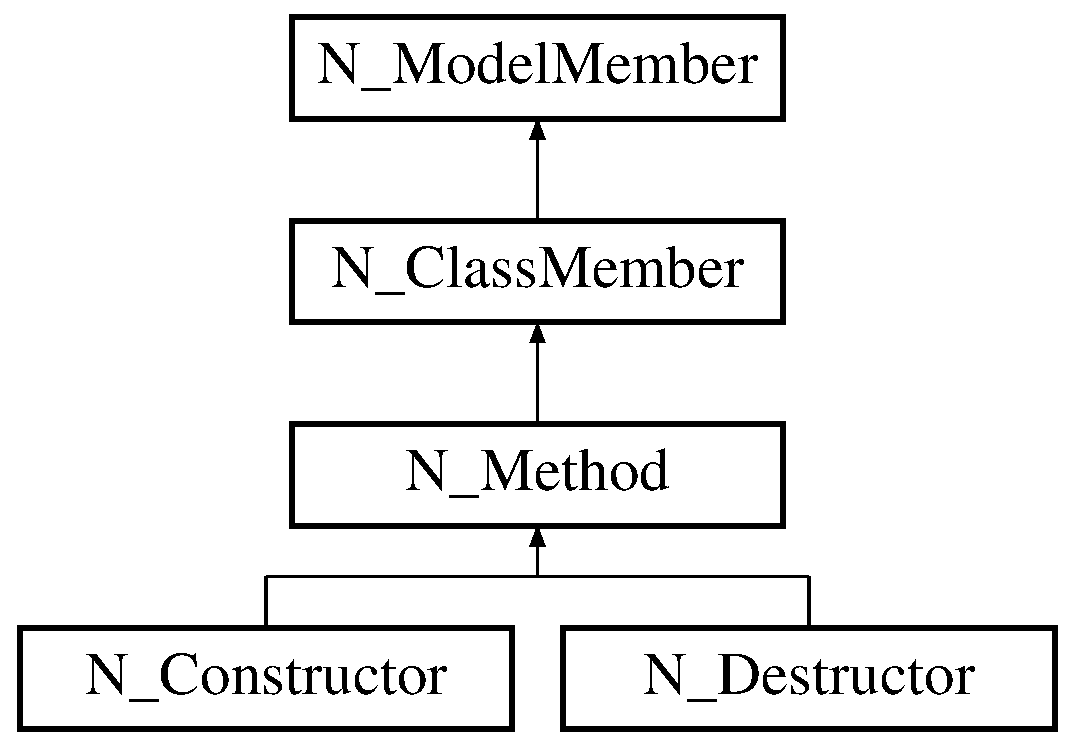
\includegraphics[height=4.000000cm]{classN__Method}
\end{center}
\end{figure}
\subsection*{Public Member Functions}
\begin{DoxyCompactItemize}
\item 
\hyperlink{classN__Method_a107d80e851cfa8d79723f78995c1c07c}{N\+\_\+\+Method} (const std\+::string \&name, const std\+::string \&type, \hyperlink{ast_8h_a8cf536792064de0e4fc620bc6f1dc90e}{Member\+Visibility} vis=\hyperlink{ast_8h_a8cf536792064de0e4fc620bc6f1dc90eae560d950ff759756c70399d8cfe015d0}{M\+V\+\_\+\+P\+R\+I\+V\+A\+T\+E})
\item 
virtual \hyperlink{classN__Method_abbaaaf1df2791d4cc1373f8c0a4d6130}{$\sim$\+N\+\_\+\+Method} ()
\item 
virtual void \hyperlink{classN__Method_a54ec9f1349dd7aa0ccf91da7cf362a2f}{add\+Param} (\hyperlink{classN__Param}{N\+\_\+\+Param} \&param)
\item 
virtual int \hyperlink{classN__Method_aa89de3b7072f61310dd0df6473020066}{get\+Param\+Count} ()
\item 
virtual void \hyperlink{classN__Method_a7df4753362b077d86945ce621586deb6}{add\+Exception} (\hyperlink{classN__Exception}{N\+\_\+\+Exception} ex)
\item 
virtual std\+::vector$<$ \hyperlink{classN__Exception}{N\+\_\+\+Exception} $>$ \hyperlink{classN__Method_abb334c1b5806d9e9f22a3565de8f0996}{get\+Exceptions} ()
\item 
virtual \hyperlink{classN__Param}{N\+\_\+\+Param} \& \hyperlink{classN__Method_a1c889024bf36ad9d4e088a6ca4581a87}{operator\mbox{[}$\,$\mbox{]}} (int n)
\end{DoxyCompactItemize}
\subsection*{Protected Attributes}
\begin{DoxyCompactItemize}
\item 
std\+::vector$<$ \hyperlink{classN__Param}{N\+\_\+\+Param} $>$ \hyperlink{classN__Method_a3c99f1955b023fff1d6a0930496beb7f}{m\+\_\+params}
\begin{DoxyCompactList}\small\item\em Коллекция параметров метода \end{DoxyCompactList}\item 
std\+::vector$<$ \hyperlink{classN__Exception}{N\+\_\+\+Exception} $>$ \hyperlink{classN__Method_aad146c11802d6e438c39377249d7b17d}{exceptions}
\begin{DoxyCompactList}\small\item\em Коллекция исключений, выкидываемых методом \end{DoxyCompactList}\end{DoxyCompactItemize}


\subsection{Detailed Description}
Нетерминал, обозначающий метод класса или интерфейса 

\subsection{Constructor \& Destructor Documentation}
\hypertarget{classN__Method_a107d80e851cfa8d79723f78995c1c07c}{}\index{N\+\_\+\+Method@{N\+\_\+\+Method}!N\+\_\+\+Method@{N\+\_\+\+Method}}
\index{N\+\_\+\+Method@{N\+\_\+\+Method}!N\+\_\+\+Method@{N\+\_\+\+Method}}
\subsubsection[{N\+\_\+\+Method}]{\setlength{\rightskip}{0pt plus 5cm}N\+\_\+\+Method\+::\+N\+\_\+\+Method (
\begin{DoxyParamCaption}
\item[{const std\+::string \&}]{name, }
\item[{const std\+::string \&}]{type, }
\item[{{\bf Member\+Visibility}}]{vis = {\ttfamily {\bf M\+V\+\_\+\+P\+R\+I\+V\+A\+T\+E}}}
\end{DoxyParamCaption}
)\hspace{0.3cm}{\ttfamily [inline]}}\label{classN__Method_a107d80e851cfa8d79723f78995c1c07c}
Конструктор 
\begin{DoxyParams}{Parameters}
{\em name} & -\/ имя метода \\
\hline
{\em type} & -\/ тип значения, возвращаемого методом \\
\hline
{\em vis} & -\/ область видимости метода \\
\hline
\end{DoxyParams}
\hypertarget{classN__Method_abbaaaf1df2791d4cc1373f8c0a4d6130}{}\index{N\+\_\+\+Method@{N\+\_\+\+Method}!````~N\+\_\+\+Method@{$\sim$\+N\+\_\+\+Method}}
\index{````~N\+\_\+\+Method@{$\sim$\+N\+\_\+\+Method}!N\+\_\+\+Method@{N\+\_\+\+Method}}
\subsubsection[{$\sim$\+N\+\_\+\+Method}]{\setlength{\rightskip}{0pt plus 5cm}virtual N\+\_\+\+Method\+::$\sim$\+N\+\_\+\+Method (
\begin{DoxyParamCaption}
{}
\end{DoxyParamCaption}
)\hspace{0.3cm}{\ttfamily [inline]}, {\ttfamily [virtual]}}\label{classN__Method_abbaaaf1df2791d4cc1373f8c0a4d6130}
Деструктор 

\subsection{Member Function Documentation}
\hypertarget{classN__Method_a7df4753362b077d86945ce621586deb6}{}\index{N\+\_\+\+Method@{N\+\_\+\+Method}!add\+Exception@{add\+Exception}}
\index{add\+Exception@{add\+Exception}!N\+\_\+\+Method@{N\+\_\+\+Method}}
\subsubsection[{add\+Exception}]{\setlength{\rightskip}{0pt plus 5cm}virtual void N\+\_\+\+Method\+::add\+Exception (
\begin{DoxyParamCaption}
\item[{{\bf N\+\_\+\+Exception}}]{ex}
\end{DoxyParamCaption}
)\hspace{0.3cm}{\ttfamily [inline]}, {\ttfamily [virtual]}}\label{classN__Method_a7df4753362b077d86945ce621586deb6}
Добавление исключения 
\begin{DoxyParams}{Parameters}
{\em ex} & -\/ исключение, которое необходимо добавить \\
\hline
\end{DoxyParams}
\hypertarget{classN__Method_a54ec9f1349dd7aa0ccf91da7cf362a2f}{}\index{N\+\_\+\+Method@{N\+\_\+\+Method}!add\+Param@{add\+Param}}
\index{add\+Param@{add\+Param}!N\+\_\+\+Method@{N\+\_\+\+Method}}
\subsubsection[{add\+Param}]{\setlength{\rightskip}{0pt plus 5cm}virtual void N\+\_\+\+Method\+::add\+Param (
\begin{DoxyParamCaption}
\item[{{\bf N\+\_\+\+Param} \&}]{param}
\end{DoxyParamCaption}
)\hspace{0.3cm}{\ttfamily [inline]}, {\ttfamily [virtual]}}\label{classN__Method_a54ec9f1349dd7aa0ccf91da7cf362a2f}
Добавление параметра метода 
\begin{DoxyParams}{Parameters}
{\em -\/} & параметр, который необходимо добавить в метод \\
\hline
\end{DoxyParams}
\hypertarget{classN__Method_abb334c1b5806d9e9f22a3565de8f0996}{}\index{N\+\_\+\+Method@{N\+\_\+\+Method}!get\+Exceptions@{get\+Exceptions}}
\index{get\+Exceptions@{get\+Exceptions}!N\+\_\+\+Method@{N\+\_\+\+Method}}
\subsubsection[{get\+Exceptions}]{\setlength{\rightskip}{0pt plus 5cm}virtual std\+::vector$<${\bf N\+\_\+\+Exception}$>$ N\+\_\+\+Method\+::get\+Exceptions (
\begin{DoxyParamCaption}
{}
\end{DoxyParamCaption}
)\hspace{0.3cm}{\ttfamily [inline]}, {\ttfamily [virtual]}}\label{classN__Method_abb334c1b5806d9e9f22a3565de8f0996}
Получение коллекции исключений, выкидываемых методом \begin{DoxyReturn}{Returns}
Коллекция исключений, выкидываемых методом 
\end{DoxyReturn}
\hypertarget{classN__Method_aa89de3b7072f61310dd0df6473020066}{}\index{N\+\_\+\+Method@{N\+\_\+\+Method}!get\+Param\+Count@{get\+Param\+Count}}
\index{get\+Param\+Count@{get\+Param\+Count}!N\+\_\+\+Method@{N\+\_\+\+Method}}
\subsubsection[{get\+Param\+Count}]{\setlength{\rightskip}{0pt plus 5cm}virtual int N\+\_\+\+Method\+::get\+Param\+Count (
\begin{DoxyParamCaption}
{}
\end{DoxyParamCaption}
)\hspace{0.3cm}{\ttfamily [inline]}, {\ttfamily [virtual]}}\label{classN__Method_aa89de3b7072f61310dd0df6473020066}
Получение количества параметров метода \begin{DoxyReturn}{Returns}
Количество параметров метода 
\end{DoxyReturn}
\hypertarget{classN__Method_a1c889024bf36ad9d4e088a6ca4581a87}{}\index{N\+\_\+\+Method@{N\+\_\+\+Method}!operator\mbox{[}$\,$\mbox{]}@{operator[]}}
\index{operator\mbox{[}$\,$\mbox{]}@{operator[]}!N\+\_\+\+Method@{N\+\_\+\+Method}}
\subsubsection[{operator[]}]{\setlength{\rightskip}{0pt plus 5cm}virtual {\bf N\+\_\+\+Param}\& N\+\_\+\+Method\+::operator\mbox{[}$\,$\mbox{]} (
\begin{DoxyParamCaption}
\item[{int}]{n}
\end{DoxyParamCaption}
)\hspace{0.3cm}{\ttfamily [inline]}, {\ttfamily [virtual]}}\label{classN__Method_a1c889024bf36ad9d4e088a6ca4581a87}
Получение параметра метода по его номеру 
\begin{DoxyParams}{Parameters}
{\em n} & -\/ номер параметра, считая от 0 \\
\hline
\end{DoxyParams}
\begin{DoxyReturn}{Returns}
Выбранный параметр метода 
\end{DoxyReturn}


\subsection{Member Data Documentation}
\hypertarget{classN__Method_aad146c11802d6e438c39377249d7b17d}{}\index{N\+\_\+\+Method@{N\+\_\+\+Method}!exceptions@{exceptions}}
\index{exceptions@{exceptions}!N\+\_\+\+Method@{N\+\_\+\+Method}}
\subsubsection[{exceptions}]{\setlength{\rightskip}{0pt plus 5cm}std\+::vector$<${\bf N\+\_\+\+Exception}$>$ N\+\_\+\+Method\+::exceptions\hspace{0.3cm}{\ttfamily [protected]}}\label{classN__Method_aad146c11802d6e438c39377249d7b17d}


Коллекция исключений, выкидываемых методом 

\hypertarget{classN__Method_a3c99f1955b023fff1d6a0930496beb7f}{}\index{N\+\_\+\+Method@{N\+\_\+\+Method}!m\+\_\+params@{m\+\_\+params}}
\index{m\+\_\+params@{m\+\_\+params}!N\+\_\+\+Method@{N\+\_\+\+Method}}
\subsubsection[{m\+\_\+params}]{\setlength{\rightskip}{0pt plus 5cm}std\+::vector$<${\bf N\+\_\+\+Param}$>$ N\+\_\+\+Method\+::m\+\_\+params\hspace{0.3cm}{\ttfamily [protected]}}\label{classN__Method_a3c99f1955b023fff1d6a0930496beb7f}


Коллекция параметров метода 



The documentation for this class was generated from the following file\+:\begin{DoxyCompactItemize}
\item 
\hyperlink{ast_8h}{ast.\+h}\end{DoxyCompactItemize}

\hypertarget{classN__Model}{}\section{N\+\_\+\+Model Class Reference}
\label{classN__Model}\index{N\+\_\+\+Model@{N\+\_\+\+Model}}


{\ttfamily \#include $<$ast.\+h$>$}

\subsection*{Public Member Functions}
\begin{DoxyCompactItemize}
\item 
\hyperlink{classN__Model_a1daec6e71b170ad19acd92a0610d3c3b}{N\+\_\+\+Model} (const std\+::string \&name)
\item 
virtual \hyperlink{classN__Model_adf9eb562be34647c3ea86c0e0977d64e}{$\sim$\+N\+\_\+\+Model} ()
\item 
virtual std\+::string \hyperlink{classN__Model_a1271bdcab31a78aef8a1de598cd3158c}{get\+Name} () const 
\item 
virtual void \hyperlink{classN__Model_ac10c3efe2443db62bbf44d3430c1298f}{add\+Member} (\hyperlink{classN__ModelMember}{N\+\_\+\+Model\+Member} $\ast$member)
\item 
virtual int \hyperlink{classN__Model_a67f00ff3575e7c7f2754dce0dc42870f}{get\+Member\+Count} () const 
\item 
virtual \hyperlink{classN__ModelMember}{N\+\_\+\+Model\+Member} $\ast$ \hyperlink{classN__Model_a0b27d0fa5410fe08b6d6564048a057db}{get\+Member} (int index)
\item 
virtual void \hyperlink{classN__Model_a6a25ea55dc864af8dc0e23829661f5c2}{add\+Option} (\hyperlink{classN__ModelOption}{N\+\_\+\+Model\+Option} \&option)
\item 
virtual int \hyperlink{classN__Model_a917f55a3f1886f77164761b3553030e5}{get\+Option\+Count} () const 
\item 
virtual \hyperlink{classN__ModelOption}{N\+\_\+\+Model\+Option} \& \hyperlink{classN__Model_a5582c8fbdbb9b7860da7c26c6be299f9}{get\+Option} (int index)
\end{DoxyCompactItemize}
\subsection*{Protected Attributes}
\begin{DoxyCompactItemize}
\item 
std\+::string \hyperlink{classN__Model_a9d9ab454862eb335a49140a4c80dcf6b}{m\+\_\+name}
\begin{DoxyCompactList}\small\item\em Имя модели \end{DoxyCompactList}\item 
std\+::vector$<$ \hyperlink{classN__ModelMember}{N\+\_\+\+Model\+Member} $\ast$ $>$ \hyperlink{classN__Model_a17c2bb912ce895df0c9e32f680a510b5}{m\+\_\+members}
\begin{DoxyCompactList}\small\item\em Коллекция элементов модели \end{DoxyCompactList}\item 
std\+::vector$<$ \hyperlink{classN__ModelOption}{N\+\_\+\+Model\+Option} $>$ \hyperlink{classN__Model_a7ef79bbb67076275fc204313c112f548}{m\+\_\+options}
\begin{DoxyCompactList}\small\item\em Коллекция опций модели \end{DoxyCompactList}\end{DoxyCompactItemize}


\subsection{Constructor \& Destructor Documentation}
\hypertarget{classN__Model_a1daec6e71b170ad19acd92a0610d3c3b}{}\index{N\+\_\+\+Model@{N\+\_\+\+Model}!N\+\_\+\+Model@{N\+\_\+\+Model}}
\index{N\+\_\+\+Model@{N\+\_\+\+Model}!N\+\_\+\+Model@{N\+\_\+\+Model}}
\subsubsection[{N\+\_\+\+Model}]{\setlength{\rightskip}{0pt plus 5cm}N\+\_\+\+Model\+::\+N\+\_\+\+Model (
\begin{DoxyParamCaption}
\item[{const std\+::string \&}]{name}
\end{DoxyParamCaption}
)\hspace{0.3cm}{\ttfamily [inline]}, {\ttfamily [explicit]}}\label{classN__Model_a1daec6e71b170ad19acd92a0610d3c3b}
Конструктор 
\begin{DoxyParams}{Parameters}
{\em name} & -\/ имя модели \\
\hline
\end{DoxyParams}
\hypertarget{classN__Model_adf9eb562be34647c3ea86c0e0977d64e}{}\index{N\+\_\+\+Model@{N\+\_\+\+Model}!````~N\+\_\+\+Model@{$\sim$\+N\+\_\+\+Model}}
\index{````~N\+\_\+\+Model@{$\sim$\+N\+\_\+\+Model}!N\+\_\+\+Model@{N\+\_\+\+Model}}
\subsubsection[{$\sim$\+N\+\_\+\+Model}]{\setlength{\rightskip}{0pt plus 5cm}virtual N\+\_\+\+Model\+::$\sim$\+N\+\_\+\+Model (
\begin{DoxyParamCaption}
{}
\end{DoxyParamCaption}
)\hspace{0.3cm}{\ttfamily [inline]}, {\ttfamily [virtual]}}\label{classN__Model_adf9eb562be34647c3ea86c0e0977d64e}
Деструктор 

\subsection{Member Function Documentation}
\hypertarget{classN__Model_ac10c3efe2443db62bbf44d3430c1298f}{}\index{N\+\_\+\+Model@{N\+\_\+\+Model}!add\+Member@{add\+Member}}
\index{add\+Member@{add\+Member}!N\+\_\+\+Model@{N\+\_\+\+Model}}
\subsubsection[{add\+Member}]{\setlength{\rightskip}{0pt plus 5cm}virtual void N\+\_\+\+Model\+::add\+Member (
\begin{DoxyParamCaption}
\item[{{\bf N\+\_\+\+Model\+Member} $\ast$}]{member}
\end{DoxyParamCaption}
)\hspace{0.3cm}{\ttfamily [inline]}, {\ttfamily [virtual]}}\label{classN__Model_ac10c3efe2443db62bbf44d3430c1298f}
Добавление элемента модели 
\begin{DoxyParams}{Parameters}
{\em member} & -\/ добавляемый элемент \\
\hline
\end{DoxyParams}
\hypertarget{classN__Model_a6a25ea55dc864af8dc0e23829661f5c2}{}\index{N\+\_\+\+Model@{N\+\_\+\+Model}!add\+Option@{add\+Option}}
\index{add\+Option@{add\+Option}!N\+\_\+\+Model@{N\+\_\+\+Model}}
\subsubsection[{add\+Option}]{\setlength{\rightskip}{0pt plus 5cm}virtual void N\+\_\+\+Model\+::add\+Option (
\begin{DoxyParamCaption}
\item[{{\bf N\+\_\+\+Model\+Option} \&}]{option}
\end{DoxyParamCaption}
)\hspace{0.3cm}{\ttfamily [inline]}, {\ttfamily [virtual]}}\label{classN__Model_a6a25ea55dc864af8dc0e23829661f5c2}
Добавление опции модели 
\begin{DoxyParams}{Parameters}
{\em option} & -\/ добавляемая опция \\
\hline
\end{DoxyParams}
\hypertarget{classN__Model_a0b27d0fa5410fe08b6d6564048a057db}{}\index{N\+\_\+\+Model@{N\+\_\+\+Model}!get\+Member@{get\+Member}}
\index{get\+Member@{get\+Member}!N\+\_\+\+Model@{N\+\_\+\+Model}}
\subsubsection[{get\+Member}]{\setlength{\rightskip}{0pt plus 5cm}virtual {\bf N\+\_\+\+Model\+Member}$\ast$ N\+\_\+\+Model\+::get\+Member (
\begin{DoxyParamCaption}
\item[{int}]{index}
\end{DoxyParamCaption}
)\hspace{0.3cm}{\ttfamily [inline]}, {\ttfamily [virtual]}}\label{classN__Model_a0b27d0fa5410fe08b6d6564048a057db}
\hypertarget{classN__Model_a67f00ff3575e7c7f2754dce0dc42870f}{}\index{N\+\_\+\+Model@{N\+\_\+\+Model}!get\+Member\+Count@{get\+Member\+Count}}
\index{get\+Member\+Count@{get\+Member\+Count}!N\+\_\+\+Model@{N\+\_\+\+Model}}
\subsubsection[{get\+Member\+Count}]{\setlength{\rightskip}{0pt plus 5cm}virtual int N\+\_\+\+Model\+::get\+Member\+Count (
\begin{DoxyParamCaption}
{}
\end{DoxyParamCaption}
) const\hspace{0.3cm}{\ttfamily [inline]}, {\ttfamily [virtual]}}\label{classN__Model_a67f00ff3575e7c7f2754dce0dc42870f}
\hypertarget{classN__Model_a1271bdcab31a78aef8a1de598cd3158c}{}\index{N\+\_\+\+Model@{N\+\_\+\+Model}!get\+Name@{get\+Name}}
\index{get\+Name@{get\+Name}!N\+\_\+\+Model@{N\+\_\+\+Model}}
\subsubsection[{get\+Name}]{\setlength{\rightskip}{0pt plus 5cm}virtual std\+::string N\+\_\+\+Model\+::get\+Name (
\begin{DoxyParamCaption}
{}
\end{DoxyParamCaption}
) const\hspace{0.3cm}{\ttfamily [inline]}, {\ttfamily [virtual]}}\label{classN__Model_a1271bdcab31a78aef8a1de598cd3158c}
Получение имени модели \begin{DoxyReturn}{Returns}
имя модели 
\end{DoxyReturn}
\hypertarget{classN__Model_a5582c8fbdbb9b7860da7c26c6be299f9}{}\index{N\+\_\+\+Model@{N\+\_\+\+Model}!get\+Option@{get\+Option}}
\index{get\+Option@{get\+Option}!N\+\_\+\+Model@{N\+\_\+\+Model}}
\subsubsection[{get\+Option}]{\setlength{\rightskip}{0pt plus 5cm}virtual {\bf N\+\_\+\+Model\+Option}\& N\+\_\+\+Model\+::get\+Option (
\begin{DoxyParamCaption}
\item[{int}]{index}
\end{DoxyParamCaption}
)\hspace{0.3cm}{\ttfamily [inline]}, {\ttfamily [virtual]}}\label{classN__Model_a5582c8fbdbb9b7860da7c26c6be299f9}
\hypertarget{classN__Model_a917f55a3f1886f77164761b3553030e5}{}\index{N\+\_\+\+Model@{N\+\_\+\+Model}!get\+Option\+Count@{get\+Option\+Count}}
\index{get\+Option\+Count@{get\+Option\+Count}!N\+\_\+\+Model@{N\+\_\+\+Model}}
\subsubsection[{get\+Option\+Count}]{\setlength{\rightskip}{0pt plus 5cm}virtual int N\+\_\+\+Model\+::get\+Option\+Count (
\begin{DoxyParamCaption}
{}
\end{DoxyParamCaption}
) const\hspace{0.3cm}{\ttfamily [inline]}, {\ttfamily [virtual]}}\label{classN__Model_a917f55a3f1886f77164761b3553030e5}


\subsection{Member Data Documentation}
\hypertarget{classN__Model_a17c2bb912ce895df0c9e32f680a510b5}{}\index{N\+\_\+\+Model@{N\+\_\+\+Model}!m\+\_\+members@{m\+\_\+members}}
\index{m\+\_\+members@{m\+\_\+members}!N\+\_\+\+Model@{N\+\_\+\+Model}}
\subsubsection[{m\+\_\+members}]{\setlength{\rightskip}{0pt plus 5cm}std\+::vector$<${\bf N\+\_\+\+Model\+Member}$\ast$$>$ N\+\_\+\+Model\+::m\+\_\+members\hspace{0.3cm}{\ttfamily [protected]}}\label{classN__Model_a17c2bb912ce895df0c9e32f680a510b5}


Коллекция элементов модели 

\hypertarget{classN__Model_a9d9ab454862eb335a49140a4c80dcf6b}{}\index{N\+\_\+\+Model@{N\+\_\+\+Model}!m\+\_\+name@{m\+\_\+name}}
\index{m\+\_\+name@{m\+\_\+name}!N\+\_\+\+Model@{N\+\_\+\+Model}}
\subsubsection[{m\+\_\+name}]{\setlength{\rightskip}{0pt plus 5cm}std\+::string N\+\_\+\+Model\+::m\+\_\+name\hspace{0.3cm}{\ttfamily [protected]}}\label{classN__Model_a9d9ab454862eb335a49140a4c80dcf6b}


Имя модели 

\hypertarget{classN__Model_a7ef79bbb67076275fc204313c112f548}{}\index{N\+\_\+\+Model@{N\+\_\+\+Model}!m\+\_\+options@{m\+\_\+options}}
\index{m\+\_\+options@{m\+\_\+options}!N\+\_\+\+Model@{N\+\_\+\+Model}}
\subsubsection[{m\+\_\+options}]{\setlength{\rightskip}{0pt plus 5cm}std\+::vector$<${\bf N\+\_\+\+Model\+Option}$>$ N\+\_\+\+Model\+::m\+\_\+options\hspace{0.3cm}{\ttfamily [protected]}}\label{classN__Model_a7ef79bbb67076275fc204313c112f548}


Коллекция опций модели 



The documentation for this class was generated from the following file\+:\begin{DoxyCompactItemize}
\item 
\hyperlink{ast_8h}{ast.\+h}\end{DoxyCompactItemize}

\hypertarget{classN__ModelMember}{}\section{N\+\_\+\+Model\+Member Class Reference}
\label{classN__ModelMember}\index{N\+\_\+\+Model\+Member@{N\+\_\+\+Model\+Member}}


{\ttfamily \#include $<$ast.\+h$>$}

Inheritance diagram for N\+\_\+\+Model\+Member\+:\begin{figure}[H]
\begin{center}
\leavevmode
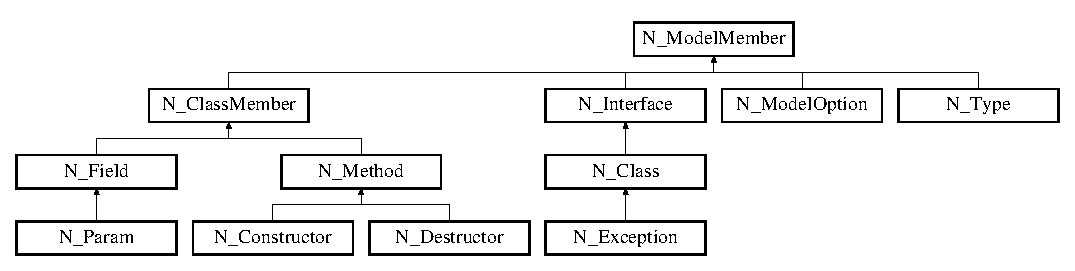
\includegraphics[height=3.190883cm]{classN__ModelMember}
\end{center}
\end{figure}
\subsection*{Public Member Functions}
\begin{DoxyCompactItemize}
\item 
\hyperlink{classN__ModelMember_ad34bba976ee6ee27b40ac4a60f6dc5e3}{N\+\_\+\+Model\+Member} (const std\+::string \&name)
\item 
virtual \hyperlink{classN__ModelMember_a4e46924533169c31720e83d1ddb8e7a1}{$\sim$\+N\+\_\+\+Model\+Member} ()
\item 
virtual std\+::string \hyperlink{classN__ModelMember_a942c73d190ee3d70fd65a57cd0ccea58}{get\+Name} () const 
\item 
virtual \hyperlink{ast_8h_a8a68ec34a59539de78ad64e57901b788}{Model\+Member\+Type} \hyperlink{classN__ModelMember_ade7ce7917050133c412d62a42453d709}{get\+Type} () const 
\end{DoxyCompactItemize}
\subsection*{Protected Attributes}
\begin{DoxyCompactItemize}
\item 
std\+::string \hyperlink{classN__ModelMember_a23a1f400b93fe4610ae59d1984195883}{m\+\_\+name}
\begin{DoxyCompactList}\small\item\em Содержит имя элемента модели \end{DoxyCompactList}\item 
\hyperlink{ast_8h_a8a68ec34a59539de78ad64e57901b788}{Model\+Member\+Type} \hyperlink{classN__ModelMember_a14c638e44cc0b3143dcb3bbf0f65dc6a}{m\+\_\+type}
\begin{DoxyCompactList}\small\item\em Содержит тип элемента модели (обход бага в R\+T\+T\+I у некоторых компиляторов) \end{DoxyCompactList}\end{DoxyCompactItemize}


\subsection{Constructor \& Destructor Documentation}
\hypertarget{classN__ModelMember_ad34bba976ee6ee27b40ac4a60f6dc5e3}{}\index{N\+\_\+\+Model\+Member@{N\+\_\+\+Model\+Member}!N\+\_\+\+Model\+Member@{N\+\_\+\+Model\+Member}}
\index{N\+\_\+\+Model\+Member@{N\+\_\+\+Model\+Member}!N\+\_\+\+Model\+Member@{N\+\_\+\+Model\+Member}}
\subsubsection[{N\+\_\+\+Model\+Member}]{\setlength{\rightskip}{0pt plus 5cm}N\+\_\+\+Model\+Member\+::\+N\+\_\+\+Model\+Member (
\begin{DoxyParamCaption}
\item[{const std\+::string \&}]{name}
\end{DoxyParamCaption}
)\hspace{0.3cm}{\ttfamily [inline]}, {\ttfamily [explicit]}}\label{classN__ModelMember_ad34bba976ee6ee27b40ac4a60f6dc5e3}
Конструктор 
\begin{DoxyParams}{Parameters}
{\em name} & -\/ имя элемента модели \\
\hline
\end{DoxyParams}
\hypertarget{classN__ModelMember_a4e46924533169c31720e83d1ddb8e7a1}{}\index{N\+\_\+\+Model\+Member@{N\+\_\+\+Model\+Member}!````~N\+\_\+\+Model\+Member@{$\sim$\+N\+\_\+\+Model\+Member}}
\index{````~N\+\_\+\+Model\+Member@{$\sim$\+N\+\_\+\+Model\+Member}!N\+\_\+\+Model\+Member@{N\+\_\+\+Model\+Member}}
\subsubsection[{$\sim$\+N\+\_\+\+Model\+Member}]{\setlength{\rightskip}{0pt plus 5cm}virtual N\+\_\+\+Model\+Member\+::$\sim$\+N\+\_\+\+Model\+Member (
\begin{DoxyParamCaption}
{}
\end{DoxyParamCaption}
)\hspace{0.3cm}{\ttfamily [inline]}, {\ttfamily [virtual]}}\label{classN__ModelMember_a4e46924533169c31720e83d1ddb8e7a1}
Деструктор 

\subsection{Member Function Documentation}
\hypertarget{classN__ModelMember_a942c73d190ee3d70fd65a57cd0ccea58}{}\index{N\+\_\+\+Model\+Member@{N\+\_\+\+Model\+Member}!get\+Name@{get\+Name}}
\index{get\+Name@{get\+Name}!N\+\_\+\+Model\+Member@{N\+\_\+\+Model\+Member}}
\subsubsection[{get\+Name}]{\setlength{\rightskip}{0pt plus 5cm}virtual std\+::string N\+\_\+\+Model\+Member\+::get\+Name (
\begin{DoxyParamCaption}
{}
\end{DoxyParamCaption}
) const\hspace{0.3cm}{\ttfamily [inline]}, {\ttfamily [virtual]}}\label{classN__ModelMember_a942c73d190ee3d70fd65a57cd0ccea58}
Получение имени элемента модели \begin{DoxyReturn}{Returns}
имя элемента модели 
\end{DoxyReturn}
\hypertarget{classN__ModelMember_ade7ce7917050133c412d62a42453d709}{}\index{N\+\_\+\+Model\+Member@{N\+\_\+\+Model\+Member}!get\+Type@{get\+Type}}
\index{get\+Type@{get\+Type}!N\+\_\+\+Model\+Member@{N\+\_\+\+Model\+Member}}
\subsubsection[{get\+Type}]{\setlength{\rightskip}{0pt plus 5cm}virtual {\bf Model\+Member\+Type} N\+\_\+\+Model\+Member\+::get\+Type (
\begin{DoxyParamCaption}
{}
\end{DoxyParamCaption}
) const\hspace{0.3cm}{\ttfamily [inline]}, {\ttfamily [virtual]}}\label{classN__ModelMember_ade7ce7917050133c412d62a42453d709}


\subsection{Member Data Documentation}
\hypertarget{classN__ModelMember_a23a1f400b93fe4610ae59d1984195883}{}\index{N\+\_\+\+Model\+Member@{N\+\_\+\+Model\+Member}!m\+\_\+name@{m\+\_\+name}}
\index{m\+\_\+name@{m\+\_\+name}!N\+\_\+\+Model\+Member@{N\+\_\+\+Model\+Member}}
\subsubsection[{m\+\_\+name}]{\setlength{\rightskip}{0pt plus 5cm}std\+::string N\+\_\+\+Model\+Member\+::m\+\_\+name\hspace{0.3cm}{\ttfamily [protected]}}\label{classN__ModelMember_a23a1f400b93fe4610ae59d1984195883}


Содержит имя элемента модели 

\hypertarget{classN__ModelMember_a14c638e44cc0b3143dcb3bbf0f65dc6a}{}\index{N\+\_\+\+Model\+Member@{N\+\_\+\+Model\+Member}!m\+\_\+type@{m\+\_\+type}}
\index{m\+\_\+type@{m\+\_\+type}!N\+\_\+\+Model\+Member@{N\+\_\+\+Model\+Member}}
\subsubsection[{m\+\_\+type}]{\setlength{\rightskip}{0pt plus 5cm}{\bf Model\+Member\+Type} N\+\_\+\+Model\+Member\+::m\+\_\+type\hspace{0.3cm}{\ttfamily [protected]}}\label{classN__ModelMember_a14c638e44cc0b3143dcb3bbf0f65dc6a}


Содержит тип элемента модели (обход бага в R\+T\+T\+I у некоторых компиляторов) 



The documentation for this class was generated from the following file\+:\begin{DoxyCompactItemize}
\item 
\hyperlink{ast_8h}{ast.\+h}\end{DoxyCompactItemize}

\hypertarget{classN__ModelOption}{}\section{N\+\_\+\+Model\+Option Class Reference}
\label{classN__ModelOption}\index{N\+\_\+\+Model\+Option@{N\+\_\+\+Model\+Option}}


{\ttfamily \#include $<$ast.\+h$>$}

Inheritance diagram for N\+\_\+\+Model\+Option\+:\begin{figure}[H]
\begin{center}
\leavevmode
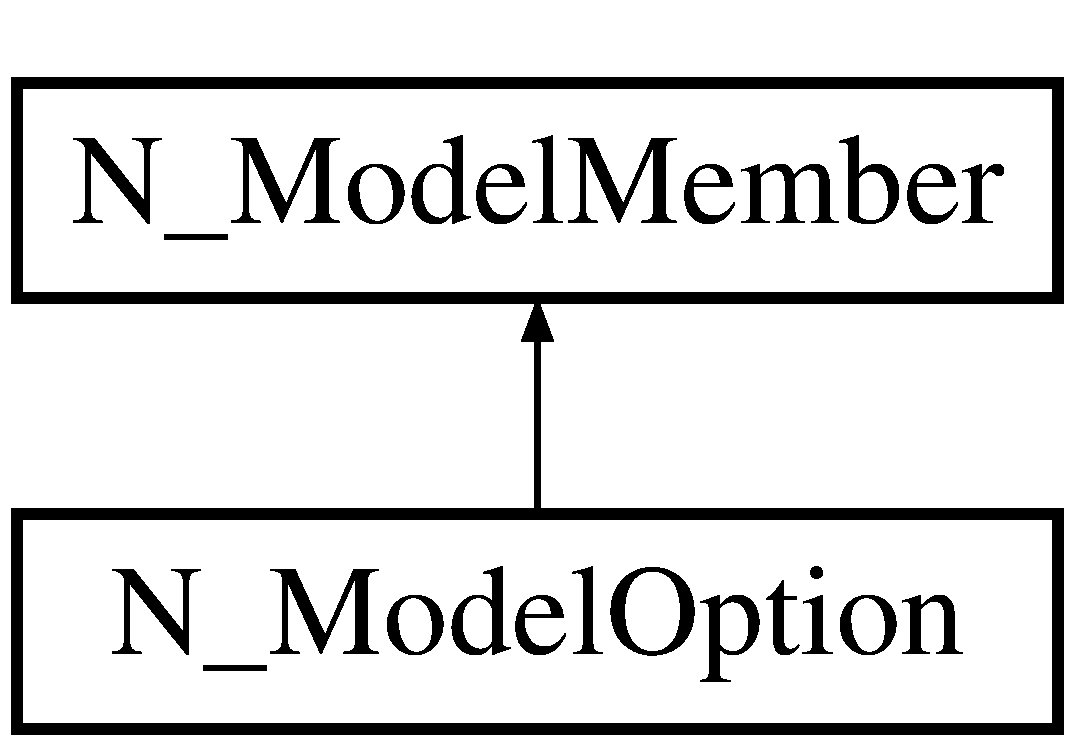
\includegraphics[height=2.000000cm]{classN__ModelOption}
\end{center}
\end{figure}
\subsection*{Public Member Functions}
\begin{DoxyCompactItemize}
\item 
\hyperlink{classN__ModelOption_ab77b5a4cde32cc2deff1c9e698d3ae42}{N\+\_\+\+Model\+Option} (const std\+::string \&name, const std\+::string \&value)
\item 
virtual \hyperlink{classN__ModelOption_aee181474459327d051cfa58af80586fb}{$\sim$\+N\+\_\+\+Model\+Option} ()
\item 
virtual std\+::string \hyperlink{classN__ModelOption_ae31bab886b932079d6754561bb155121}{get\+Value} () const 
\end{DoxyCompactItemize}
\subsection*{Protected Attributes}
\begin{DoxyCompactItemize}
\item 
std\+::string \hyperlink{classN__ModelOption_ad618798d401e3856f027ba7856359dd7}{m\+\_\+value}
\begin{DoxyCompactList}\small\item\em Содержит значение опции \end{DoxyCompactList}\end{DoxyCompactItemize}


\subsection{Constructor \& Destructor Documentation}
\hypertarget{classN__ModelOption_ab77b5a4cde32cc2deff1c9e698d3ae42}{}\index{N\+\_\+\+Model\+Option@{N\+\_\+\+Model\+Option}!N\+\_\+\+Model\+Option@{N\+\_\+\+Model\+Option}}
\index{N\+\_\+\+Model\+Option@{N\+\_\+\+Model\+Option}!N\+\_\+\+Model\+Option@{N\+\_\+\+Model\+Option}}
\subsubsection[{N\+\_\+\+Model\+Option}]{\setlength{\rightskip}{0pt plus 5cm}N\+\_\+\+Model\+Option\+::\+N\+\_\+\+Model\+Option (
\begin{DoxyParamCaption}
\item[{const std\+::string \&}]{name, }
\item[{const std\+::string \&}]{value}
\end{DoxyParamCaption}
)\hspace{0.3cm}{\ttfamily [inline]}}\label{classN__ModelOption_ab77b5a4cde32cc2deff1c9e698d3ae42}
Конструктор 
\begin{DoxyParams}{Parameters}
{\em name} & -\/ имя опции \\
\hline
{\em value} & -\/ значение опции \\
\hline
\end{DoxyParams}
\hypertarget{classN__ModelOption_aee181474459327d051cfa58af80586fb}{}\index{N\+\_\+\+Model\+Option@{N\+\_\+\+Model\+Option}!````~N\+\_\+\+Model\+Option@{$\sim$\+N\+\_\+\+Model\+Option}}
\index{````~N\+\_\+\+Model\+Option@{$\sim$\+N\+\_\+\+Model\+Option}!N\+\_\+\+Model\+Option@{N\+\_\+\+Model\+Option}}
\subsubsection[{$\sim$\+N\+\_\+\+Model\+Option}]{\setlength{\rightskip}{0pt plus 5cm}virtual N\+\_\+\+Model\+Option\+::$\sim$\+N\+\_\+\+Model\+Option (
\begin{DoxyParamCaption}
{}
\end{DoxyParamCaption}
)\hspace{0.3cm}{\ttfamily [inline]}, {\ttfamily [virtual]}}\label{classN__ModelOption_aee181474459327d051cfa58af80586fb}
Деструктор 

\subsection{Member Function Documentation}
\hypertarget{classN__ModelOption_ae31bab886b932079d6754561bb155121}{}\index{N\+\_\+\+Model\+Option@{N\+\_\+\+Model\+Option}!get\+Value@{get\+Value}}
\index{get\+Value@{get\+Value}!N\+\_\+\+Model\+Option@{N\+\_\+\+Model\+Option}}
\subsubsection[{get\+Value}]{\setlength{\rightskip}{0pt plus 5cm}virtual std\+::string N\+\_\+\+Model\+Option\+::get\+Value (
\begin{DoxyParamCaption}
{}
\end{DoxyParamCaption}
) const\hspace{0.3cm}{\ttfamily [inline]}, {\ttfamily [virtual]}}\label{classN__ModelOption_ae31bab886b932079d6754561bb155121}
Получение значение опции \begin{DoxyReturn}{Returns}
значение опции 
\end{DoxyReturn}


\subsection{Member Data Documentation}
\hypertarget{classN__ModelOption_ad618798d401e3856f027ba7856359dd7}{}\index{N\+\_\+\+Model\+Option@{N\+\_\+\+Model\+Option}!m\+\_\+value@{m\+\_\+value}}
\index{m\+\_\+value@{m\+\_\+value}!N\+\_\+\+Model\+Option@{N\+\_\+\+Model\+Option}}
\subsubsection[{m\+\_\+value}]{\setlength{\rightskip}{0pt plus 5cm}std\+::string N\+\_\+\+Model\+Option\+::m\+\_\+value\hspace{0.3cm}{\ttfamily [protected]}}\label{classN__ModelOption_ad618798d401e3856f027ba7856359dd7}


Содержит значение опции 



The documentation for this class was generated from the following file\+:\begin{DoxyCompactItemize}
\item 
\hyperlink{ast_8h}{ast.\+h}\end{DoxyCompactItemize}

\hypertarget{classN__Param}{}\section{N\+\_\+\+Param Class Reference}
\label{classN__Param}\index{N\+\_\+\+Param@{N\+\_\+\+Param}}


{\ttfamily \#include $<$ast.\+h$>$}

Inheritance diagram for N\+\_\+\+Param\+:\begin{figure}[H]
\begin{center}
\leavevmode
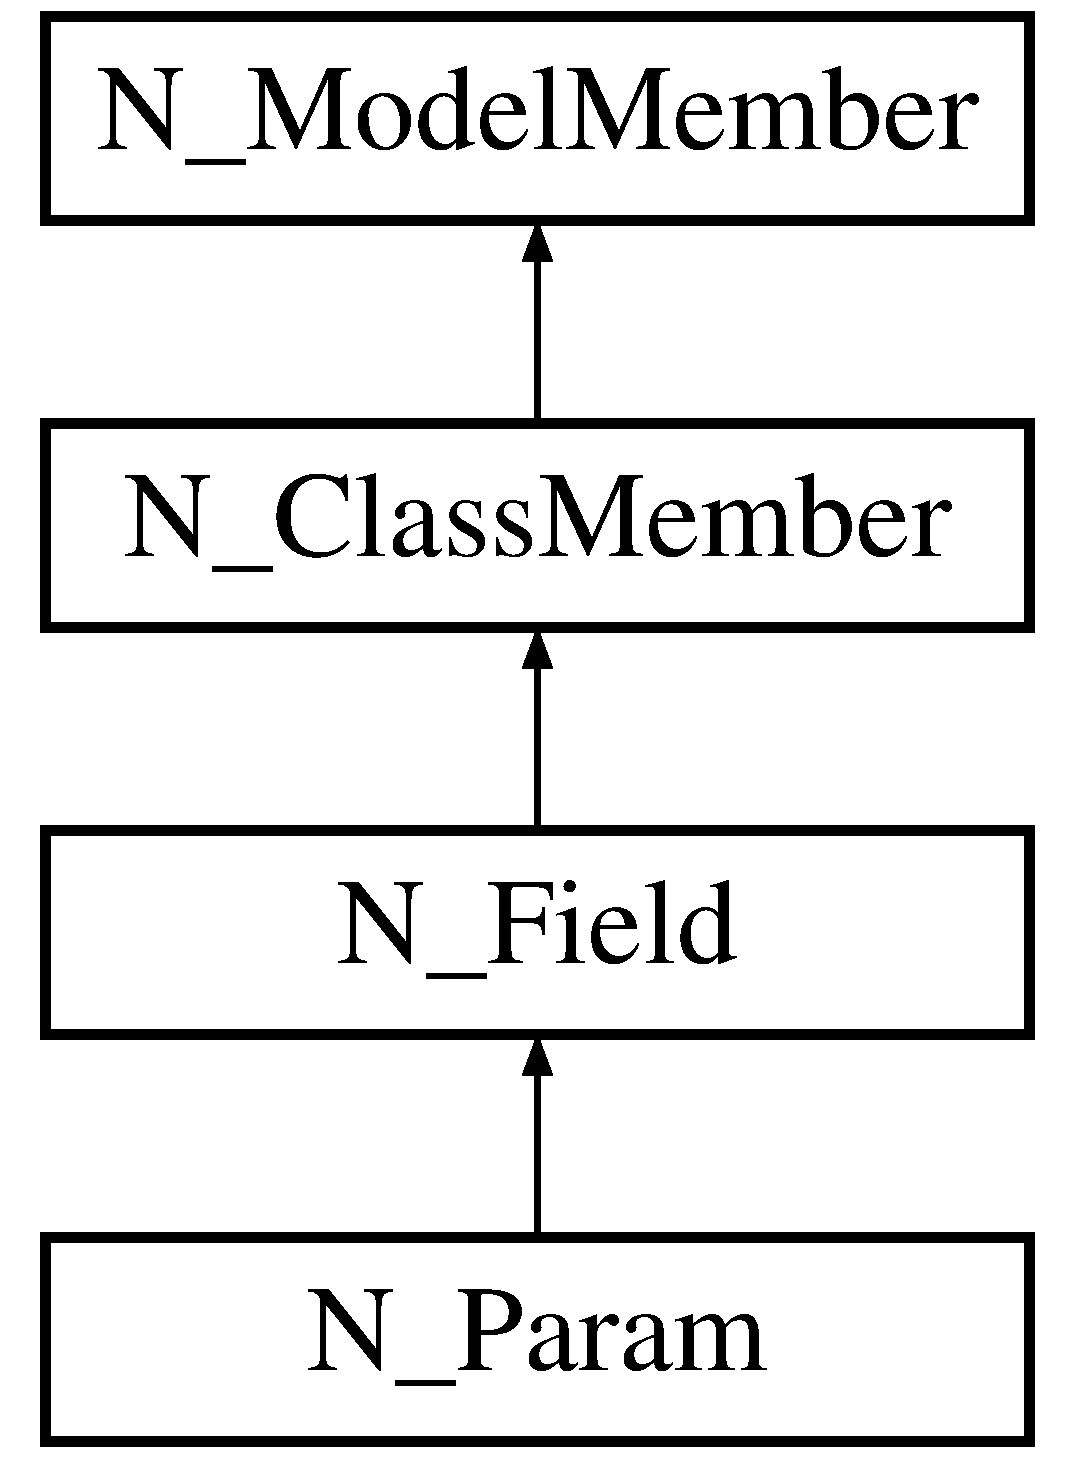
\includegraphics[height=4.000000cm]{classN__Param}
\end{center}
\end{figure}
\subsection*{Public Member Functions}
\begin{DoxyCompactItemize}
\item 
\hyperlink{classN__Param_a139b2cfde8b6ee552a3d745923385e8a}{N\+\_\+\+Param} (const std\+::string \&name, const std\+::string \&type, \hyperlink{ast_8h_af1bb1892f9e576501ff47410367569a7}{Param\+Direction} dir=\hyperlink{ast_8h_af1bb1892f9e576501ff47410367569a7afee394973f2e8a09ef035ae90b3eadb8}{F\+D\+\_\+\+I\+N})
\item 
virtual \hyperlink{classN__Param_a6210fdea783f436c304f238a011147b8}{$\sim$\+N\+\_\+\+Param} ()
\item 
virtual \hyperlink{ast_8h_af1bb1892f9e576501ff47410367569a7}{Param\+Direction} \hyperlink{classN__Param_a7bb8f5849bebadae38ea4972fdc57dc8}{get\+Direction} ()
\end{DoxyCompactItemize}
\subsection*{Protected Attributes}
\begin{DoxyCompactItemize}
\item 
\hyperlink{ast_8h_af1bb1892f9e576501ff47410367569a7}{Param\+Direction} \hyperlink{classN__Param_a72e88bb3b11584177bae2b66e009f9fb}{m\+\_\+dir}
\begin{DoxyCompactList}\small\item\em Направление параметра \end{DoxyCompactList}\end{DoxyCompactItemize}
\subsection*{Private Member Functions}
\begin{DoxyCompactItemize}
\item 
virtual \hyperlink{ast_8h_a8cf536792064de0e4fc620bc6f1dc90e}{Member\+Visibility} \hyperlink{classN__Param_a296887c43afee1fc7ccfc63f345d4427}{get\+Visibility} ()=delete
\end{DoxyCompactItemize}


\subsection{Detailed Description}
Параметр метода 

\subsection{Constructor \& Destructor Documentation}
\hypertarget{classN__Param_a139b2cfde8b6ee552a3d745923385e8a}{}\index{N\+\_\+\+Param@{N\+\_\+\+Param}!N\+\_\+\+Param@{N\+\_\+\+Param}}
\index{N\+\_\+\+Param@{N\+\_\+\+Param}!N\+\_\+\+Param@{N\+\_\+\+Param}}
\subsubsection[{N\+\_\+\+Param}]{\setlength{\rightskip}{0pt plus 5cm}N\+\_\+\+Param\+::\+N\+\_\+\+Param (
\begin{DoxyParamCaption}
\item[{const std\+::string \&}]{name, }
\item[{const std\+::string \&}]{type, }
\item[{{\bf Param\+Direction}}]{dir = {\ttfamily {\bf F\+D\+\_\+\+I\+N}}}
\end{DoxyParamCaption}
)\hspace{0.3cm}{\ttfamily [inline]}}\label{classN__Param_a139b2cfde8b6ee552a3d745923385e8a}
Конструктор 
\begin{DoxyParams}{Parameters}
{\em name} & -\/ имя параметра \\
\hline
{\em type} & -\/ тип параметра \\
\hline
{\em dir} & -\/ направление параметра \\
\hline
\end{DoxyParams}
\hypertarget{classN__Param_a6210fdea783f436c304f238a011147b8}{}\index{N\+\_\+\+Param@{N\+\_\+\+Param}!````~N\+\_\+\+Param@{$\sim$\+N\+\_\+\+Param}}
\index{````~N\+\_\+\+Param@{$\sim$\+N\+\_\+\+Param}!N\+\_\+\+Param@{N\+\_\+\+Param}}
\subsubsection[{$\sim$\+N\+\_\+\+Param}]{\setlength{\rightskip}{0pt plus 5cm}virtual N\+\_\+\+Param\+::$\sim$\+N\+\_\+\+Param (
\begin{DoxyParamCaption}
{}
\end{DoxyParamCaption}
)\hspace{0.3cm}{\ttfamily [inline]}, {\ttfamily [virtual]}}\label{classN__Param_a6210fdea783f436c304f238a011147b8}
Деструктор 

\subsection{Member Function Documentation}
\hypertarget{classN__Param_a7bb8f5849bebadae38ea4972fdc57dc8}{}\index{N\+\_\+\+Param@{N\+\_\+\+Param}!get\+Direction@{get\+Direction}}
\index{get\+Direction@{get\+Direction}!N\+\_\+\+Param@{N\+\_\+\+Param}}
\subsubsection[{get\+Direction}]{\setlength{\rightskip}{0pt plus 5cm}virtual {\bf Param\+Direction} N\+\_\+\+Param\+::get\+Direction (
\begin{DoxyParamCaption}
{}
\end{DoxyParamCaption}
)\hspace{0.3cm}{\ttfamily [inline]}, {\ttfamily [virtual]}}\label{classN__Param_a7bb8f5849bebadae38ea4972fdc57dc8}
Получение направления параметра \begin{DoxyReturn}{Returns}
Направление параметра 
\end{DoxyReturn}
\hypertarget{classN__Param_a296887c43afee1fc7ccfc63f345d4427}{}\index{N\+\_\+\+Param@{N\+\_\+\+Param}!get\+Visibility@{get\+Visibility}}
\index{get\+Visibility@{get\+Visibility}!N\+\_\+\+Param@{N\+\_\+\+Param}}
\subsubsection[{get\+Visibility}]{\setlength{\rightskip}{0pt plus 5cm}virtual {\bf Member\+Visibility} N\+\_\+\+Param\+::get\+Visibility (
\begin{DoxyParamCaption}
{}
\end{DoxyParamCaption}
)\hspace{0.3cm}{\ttfamily [private]}, {\ttfamily [virtual]}, {\ttfamily [delete]}}\label{classN__Param_a296887c43afee1fc7ccfc63f345d4427}
Получение области видимости параметра. Поскольку таковой не существует, метод предка скрыт. 

\subsection{Member Data Documentation}
\hypertarget{classN__Param_a72e88bb3b11584177bae2b66e009f9fb}{}\index{N\+\_\+\+Param@{N\+\_\+\+Param}!m\+\_\+dir@{m\+\_\+dir}}
\index{m\+\_\+dir@{m\+\_\+dir}!N\+\_\+\+Param@{N\+\_\+\+Param}}
\subsubsection[{m\+\_\+dir}]{\setlength{\rightskip}{0pt plus 5cm}{\bf Param\+Direction} N\+\_\+\+Param\+::m\+\_\+dir\hspace{0.3cm}{\ttfamily [protected]}}\label{classN__Param_a72e88bb3b11584177bae2b66e009f9fb}


Направление параметра 



The documentation for this class was generated from the following file\+:\begin{DoxyCompactItemize}
\item 
\hyperlink{ast_8h}{ast.\+h}\end{DoxyCompactItemize}

\hypertarget{classN__Type}{}\section{N\+\_\+\+Type Class Reference}
\label{classN__Type}\index{N\+\_\+\+Type@{N\+\_\+\+Type}}


{\ttfamily \#include $<$ast.\+h$>$}

Inheritance diagram for N\+\_\+\+Type\+:\begin{figure}[H]
\begin{center}
\leavevmode
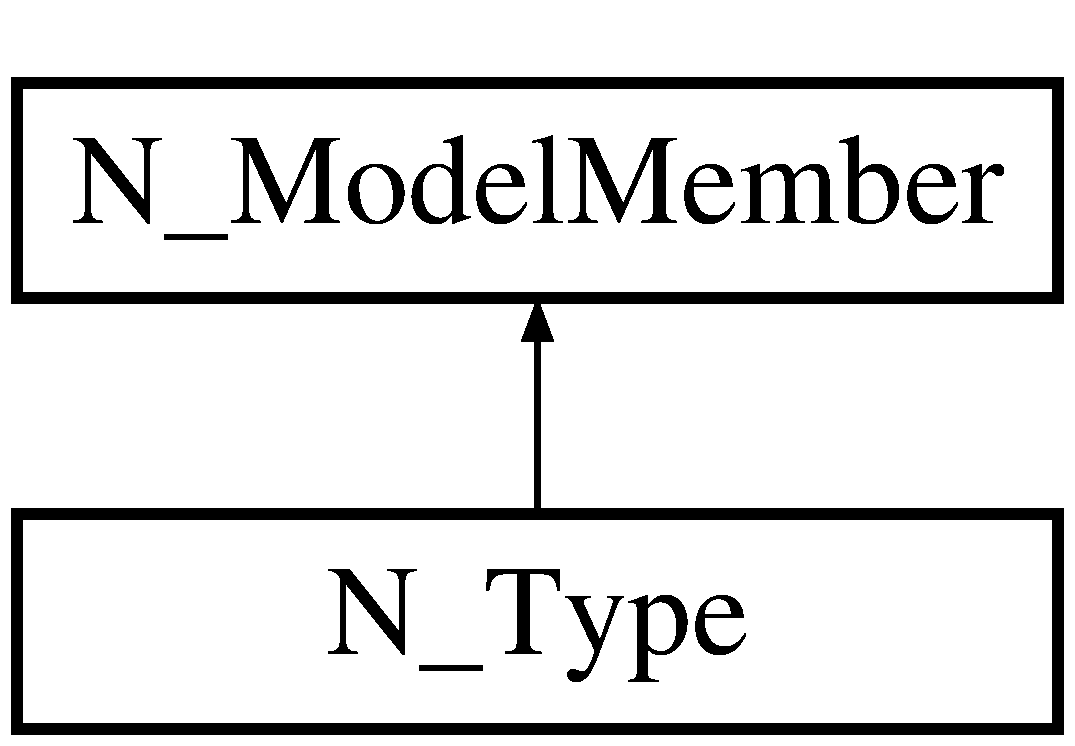
\includegraphics[height=2.000000cm]{classN__Type}
\end{center}
\end{figure}
\subsection*{Public Member Functions}
\begin{DoxyCompactItemize}
\item 
\hyperlink{classN__Type_acb49f4ac3823f81476aecdc786912927}{N\+\_\+\+Type} (const std\+::string \&name)
\item 
\hyperlink{classN__Type_aaadb2c45fb50a87d4bc9e38690606ed5}{N\+\_\+\+Type} (const std\+::string \&name, const std\+::string \&original)
\item 
\hyperlink{classN__Type_a3e032190309b0fa6c2f952248693229c}{N\+\_\+\+Type} (const \hyperlink{classN__Type}{N\+\_\+\+Type} \&t)
\item 
virtual \hyperlink{classN__Type_a1e16bc2b69f6604bea8f0938717645e7}{$\sim$\+N\+\_\+\+Type} ()
\item 
virtual std\+::string \hyperlink{classN__Type_afc6dd4daafea765545a116847ebae9e7}{get\+Aliased\+Type} () const 
\item 
virtual bool \hyperlink{classN__Type_a5b3d5eb542b6fd1976d85308eaa88c8e}{is\+Builtin} () const 
\end{DoxyCompactItemize}
\subsection*{Protected Attributes}
\begin{DoxyCompactItemize}
\item 
bool \hyperlink{classN__Type_af024de34517a3d91855aa863b8954f75}{m\+\_\+builtin}
\begin{DoxyCompactList}\small\item\em Является ли тип встроенным \end{DoxyCompactList}\item 
std\+::string \hyperlink{classN__Type_a3498f93c81b4c579e16b6ba70cb957b8}{m\+\_\+aliased\+\_\+type}
\begin{DoxyCompactList}\small\item\em Исходный тип \end{DoxyCompactList}\end{DoxyCompactItemize}


\subsection{Detailed Description}
Нетерминал, обозначающий тип данных 

\subsection{Constructor \& Destructor Documentation}
\hypertarget{classN__Type_acb49f4ac3823f81476aecdc786912927}{}\index{N\+\_\+\+Type@{N\+\_\+\+Type}!N\+\_\+\+Type@{N\+\_\+\+Type}}
\index{N\+\_\+\+Type@{N\+\_\+\+Type}!N\+\_\+\+Type@{N\+\_\+\+Type}}
\subsubsection[{N\+\_\+\+Type}]{\setlength{\rightskip}{0pt plus 5cm}N\+\_\+\+Type\+::\+N\+\_\+\+Type (
\begin{DoxyParamCaption}
\item[{const std\+::string \&}]{name}
\end{DoxyParamCaption}
)\hspace{0.3cm}{\ttfamily [inline]}, {\ttfamily [explicit]}}\label{classN__Type_acb49f4ac3823f81476aecdc786912927}
Конструктор встроенного типа 
\begin{DoxyParams}{Parameters}
{\em name} & -\/ имя типа данных \\
\hline
\end{DoxyParams}
\hypertarget{classN__Type_aaadb2c45fb50a87d4bc9e38690606ed5}{}\index{N\+\_\+\+Type@{N\+\_\+\+Type}!N\+\_\+\+Type@{N\+\_\+\+Type}}
\index{N\+\_\+\+Type@{N\+\_\+\+Type}!N\+\_\+\+Type@{N\+\_\+\+Type}}
\subsubsection[{N\+\_\+\+Type}]{\setlength{\rightskip}{0pt plus 5cm}N\+\_\+\+Type\+::\+N\+\_\+\+Type (
\begin{DoxyParamCaption}
\item[{const std\+::string \&}]{name, }
\item[{const std\+::string \&}]{original}
\end{DoxyParamCaption}
)\hspace{0.3cm}{\ttfamily [inline]}}\label{classN__Type_aaadb2c45fb50a87d4bc9e38690606ed5}
Конструктор типа-\/псевдонима 
\begin{DoxyParams}{Parameters}
{\em name} & -\/ имя типа данных \\
\hline
{\em original} & -\/ имя исходного типа \\
\hline
\end{DoxyParams}
\hypertarget{classN__Type_a3e032190309b0fa6c2f952248693229c}{}\index{N\+\_\+\+Type@{N\+\_\+\+Type}!N\+\_\+\+Type@{N\+\_\+\+Type}}
\index{N\+\_\+\+Type@{N\+\_\+\+Type}!N\+\_\+\+Type@{N\+\_\+\+Type}}
\subsubsection[{N\+\_\+\+Type}]{\setlength{\rightskip}{0pt plus 5cm}N\+\_\+\+Type\+::\+N\+\_\+\+Type (
\begin{DoxyParamCaption}
\item[{const {\bf N\+\_\+\+Type} \&}]{t}
\end{DoxyParamCaption}
)\hspace{0.3cm}{\ttfamily [inline]}}\label{classN__Type_a3e032190309b0fa6c2f952248693229c}
Копирующий конструктор 
\begin{DoxyParams}{Parameters}
{\em t} & -\/ оригинальный экземпляр \\
\hline
\end{DoxyParams}
\hypertarget{classN__Type_a1e16bc2b69f6604bea8f0938717645e7}{}\index{N\+\_\+\+Type@{N\+\_\+\+Type}!````~N\+\_\+\+Type@{$\sim$\+N\+\_\+\+Type}}
\index{````~N\+\_\+\+Type@{$\sim$\+N\+\_\+\+Type}!N\+\_\+\+Type@{N\+\_\+\+Type}}
\subsubsection[{$\sim$\+N\+\_\+\+Type}]{\setlength{\rightskip}{0pt plus 5cm}virtual N\+\_\+\+Type\+::$\sim$\+N\+\_\+\+Type (
\begin{DoxyParamCaption}
{}
\end{DoxyParamCaption}
)\hspace{0.3cm}{\ttfamily [inline]}, {\ttfamily [virtual]}}\label{classN__Type_a1e16bc2b69f6604bea8f0938717645e7}
Деструктор 

\subsection{Member Function Documentation}
\hypertarget{classN__Type_afc6dd4daafea765545a116847ebae9e7}{}\index{N\+\_\+\+Type@{N\+\_\+\+Type}!get\+Aliased\+Type@{get\+Aliased\+Type}}
\index{get\+Aliased\+Type@{get\+Aliased\+Type}!N\+\_\+\+Type@{N\+\_\+\+Type}}
\subsubsection[{get\+Aliased\+Type}]{\setlength{\rightskip}{0pt plus 5cm}virtual std\+::string N\+\_\+\+Type\+::get\+Aliased\+Type (
\begin{DoxyParamCaption}
{}
\end{DoxyParamCaption}
) const\hspace{0.3cm}{\ttfamily [inline]}, {\ttfamily [virtual]}}\label{classN__Type_afc6dd4daafea765545a116847ebae9e7}
Получение имени исходного типа \begin{DoxyReturn}{Returns}
имя исходного типа 
\end{DoxyReturn}
\hypertarget{classN__Type_a5b3d5eb542b6fd1976d85308eaa88c8e}{}\index{N\+\_\+\+Type@{N\+\_\+\+Type}!is\+Builtin@{is\+Builtin}}
\index{is\+Builtin@{is\+Builtin}!N\+\_\+\+Type@{N\+\_\+\+Type}}
\subsubsection[{is\+Builtin}]{\setlength{\rightskip}{0pt plus 5cm}virtual bool N\+\_\+\+Type\+::is\+Builtin (
\begin{DoxyParamCaption}
{}
\end{DoxyParamCaption}
) const\hspace{0.3cm}{\ttfamily [inline]}, {\ttfamily [virtual]}}\label{classN__Type_a5b3d5eb542b6fd1976d85308eaa88c8e}
Является ли тип встроенным \begin{DoxyReturn}{Returns}
true, если тип встроенный, иначе false 
\end{DoxyReturn}


\subsection{Member Data Documentation}
\hypertarget{classN__Type_a3498f93c81b4c579e16b6ba70cb957b8}{}\index{N\+\_\+\+Type@{N\+\_\+\+Type}!m\+\_\+aliased\+\_\+type@{m\+\_\+aliased\+\_\+type}}
\index{m\+\_\+aliased\+\_\+type@{m\+\_\+aliased\+\_\+type}!N\+\_\+\+Type@{N\+\_\+\+Type}}
\subsubsection[{m\+\_\+aliased\+\_\+type}]{\setlength{\rightskip}{0pt plus 5cm}std\+::string N\+\_\+\+Type\+::m\+\_\+aliased\+\_\+type\hspace{0.3cm}{\ttfamily [protected]}}\label{classN__Type_a3498f93c81b4c579e16b6ba70cb957b8}


Исходный тип 

\hypertarget{classN__Type_af024de34517a3d91855aa863b8954f75}{}\index{N\+\_\+\+Type@{N\+\_\+\+Type}!m\+\_\+builtin@{m\+\_\+builtin}}
\index{m\+\_\+builtin@{m\+\_\+builtin}!N\+\_\+\+Type@{N\+\_\+\+Type}}
\subsubsection[{m\+\_\+builtin}]{\setlength{\rightskip}{0pt plus 5cm}bool N\+\_\+\+Type\+::m\+\_\+builtin\hspace{0.3cm}{\ttfamily [protected]}}\label{classN__Type_af024de34517a3d91855aa863b8954f75}


Является ли тип встроенным 



The documentation for this class was generated from the following file\+:\begin{DoxyCompactItemize}
\item 
\hyperlink{ast_8h}{ast.\+h}\end{DoxyCompactItemize}

\hypertarget{classObjPascalGenerator}{}\section{Obj\+Pascal\+Generator Class Reference}
\label{classObjPascalGenerator}\index{Obj\+Pascal\+Generator@{Obj\+Pascal\+Generator}}


{\ttfamily \#include $<$ast.\+h$>$}

Inheritance diagram for Obj\+Pascal\+Generator\+:\begin{figure}[H]
\begin{center}
\leavevmode
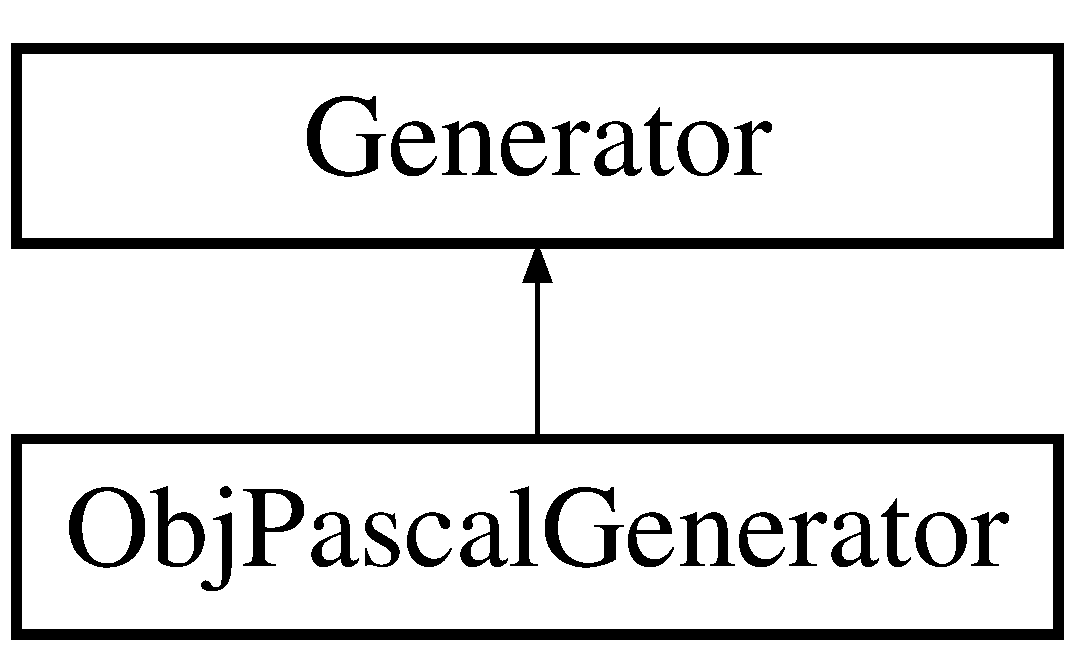
\includegraphics[height=2.000000cm]{classObjPascalGenerator}
\end{center}
\end{figure}
\subsection*{Public Member Functions}
\begin{DoxyCompactItemize}
\item 
virtual \hyperlink{classObjPascalGenerator_a83c889dac4b29dc7979fbf06fc0fe06a}{$\sim$\+Obj\+Pascal\+Generator} ()
\item 
virtual void \hyperlink{classObjPascalGenerator_a8129a8aab5c9b1f8dab3bb3c4de460d0}{generate} (\hyperlink{classN__Model}{N\+\_\+\+Model} \&m)
\item 
virtual std\+::string \hyperlink{classObjPascalGenerator_a833b2caffb9da2595a9f447bc6264ecf}{gen\+Interface} (\hyperlink{classN__Interface}{N\+\_\+\+Interface} $\ast$c)
\item 
virtual std\+::string \hyperlink{classObjPascalGenerator_a0bb3fad2c4df2a741c96d37d1e2d4449}{gen\+Field} (\hyperlink{classN__Field}{N\+\_\+\+Field} $\ast$f)
\item 
virtual std\+::string \hyperlink{classObjPascalGenerator_a4fa9c56ef03cc1999ce178fabedebb60}{gen\+Method} (\hyperlink{classN__Method}{N\+\_\+\+Method} $\ast$m)
\item 
virtual std\+::string \hyperlink{classObjPascalGenerator_a1c6095fef516716336de164da25da1e2}{gen\+Method\+Header} (\hyperlink{classN__Method}{N\+\_\+\+Method} $\ast$m)
\item 
virtual std\+::string \hyperlink{classObjPascalGenerator_a1f6ec48b26e0a002816737220a6eb26d}{gen\+Parameter} (\hyperlink{classN__Param}{N\+\_\+\+Param} $\ast$p)
\item 
virtual std\+::string \hyperlink{classObjPascalGenerator_a690ce15adcc6d94fc994737f1acdfac7}{gen\+Class} (\hyperlink{classN__Class}{N\+\_\+\+Class} $\ast$c)
\end{DoxyCompactItemize}
\subsection*{Protected Member Functions}
\begin{DoxyCompactItemize}
\item 
\hyperlink{classObjPascalGenerator_ab69aa8ddff1ff4b2a087e1988c206ae7}{Obj\+Pascal\+Generator} (std\+::ostream \&os)
\end{DoxyCompactItemize}
\subsection*{Friends}
\begin{DoxyCompactItemize}
\item 
class \hyperlink{classObjPascalGenerator_a366b7823e659ab78d952a7d79662a4d6}{Generator}
\end{DoxyCompactItemize}
\subsection*{Additional Inherited Members}


\subsection{Detailed Description}
Генератор кода на Object\+Pascal 

\subsection{Constructor \& Destructor Documentation}
\hypertarget{classObjPascalGenerator_ab69aa8ddff1ff4b2a087e1988c206ae7}{}\index{Obj\+Pascal\+Generator@{Obj\+Pascal\+Generator}!Obj\+Pascal\+Generator@{Obj\+Pascal\+Generator}}
\index{Obj\+Pascal\+Generator@{Obj\+Pascal\+Generator}!Obj\+Pascal\+Generator@{Obj\+Pascal\+Generator}}
\subsubsection[{Obj\+Pascal\+Generator}]{\setlength{\rightskip}{0pt plus 5cm}Obj\+Pascal\+Generator\+::\+Obj\+Pascal\+Generator (
\begin{DoxyParamCaption}
\item[{std\+::ostream \&}]{os}
\end{DoxyParamCaption}
)\hspace{0.3cm}{\ttfamily [inline]}, {\ttfamily [protected]}}\label{classObjPascalGenerator_ab69aa8ddff1ff4b2a087e1988c206ae7}
\hypertarget{classObjPascalGenerator_a83c889dac4b29dc7979fbf06fc0fe06a}{}\index{Obj\+Pascal\+Generator@{Obj\+Pascal\+Generator}!````~Obj\+Pascal\+Generator@{$\sim$\+Obj\+Pascal\+Generator}}
\index{````~Obj\+Pascal\+Generator@{$\sim$\+Obj\+Pascal\+Generator}!Obj\+Pascal\+Generator@{Obj\+Pascal\+Generator}}
\subsubsection[{$\sim$\+Obj\+Pascal\+Generator}]{\setlength{\rightskip}{0pt plus 5cm}virtual Obj\+Pascal\+Generator\+::$\sim$\+Obj\+Pascal\+Generator (
\begin{DoxyParamCaption}
{}
\end{DoxyParamCaption}
)\hspace{0.3cm}{\ttfamily [inline]}, {\ttfamily [virtual]}}\label{classObjPascalGenerator_a83c889dac4b29dc7979fbf06fc0fe06a}


\subsection{Member Function Documentation}
\hypertarget{classObjPascalGenerator_a690ce15adcc6d94fc994737f1acdfac7}{}\index{Obj\+Pascal\+Generator@{Obj\+Pascal\+Generator}!gen\+Class@{gen\+Class}}
\index{gen\+Class@{gen\+Class}!Obj\+Pascal\+Generator@{Obj\+Pascal\+Generator}}
\subsubsection[{gen\+Class}]{\setlength{\rightskip}{0pt plus 5cm}std\+::string Obj\+Pascal\+Generator\+::gen\+Class (
\begin{DoxyParamCaption}
\item[{{\bf N\+\_\+\+Class} $\ast$}]{c}
\end{DoxyParamCaption}
)\hspace{0.3cm}{\ttfamily [virtual]}}\label{classObjPascalGenerator_a690ce15adcc6d94fc994737f1acdfac7}
Генератор шаблона класса 
\begin{DoxyParams}{Parameters}
{\em c} & -\/ класс, для которого необходимо сгенерировать шаблон \\
\hline
\end{DoxyParams}
\begin{DoxyReturn}{Returns}
Сгенерированный шаблон 
\end{DoxyReturn}


Implements \hyperlink{classGenerator_afac361fceae302fb09e8170d097415d4}{Generator}.

\hypertarget{classObjPascalGenerator_a8129a8aab5c9b1f8dab3bb3c4de460d0}{}\index{Obj\+Pascal\+Generator@{Obj\+Pascal\+Generator}!generate@{generate}}
\index{generate@{generate}!Obj\+Pascal\+Generator@{Obj\+Pascal\+Generator}}
\subsubsection[{generate}]{\setlength{\rightskip}{0pt plus 5cm}void Obj\+Pascal\+Generator\+::generate (
\begin{DoxyParamCaption}
\item[{{\bf N\+\_\+\+Model} \&}]{m}
\end{DoxyParamCaption}
)\hspace{0.3cm}{\ttfamily [virtual]}}\label{classObjPascalGenerator_a8129a8aab5c9b1f8dab3bb3c4de460d0}
Генератор шаблона модели 
\begin{DoxyParams}{Parameters}
{\em m} & -\/ модель, для которой необходимо сгенерировать шаблон \\
\hline
\end{DoxyParams}


Implements \hyperlink{classGenerator_a518161ca79e68d733687f8e2985abd16}{Generator}.

\hypertarget{classObjPascalGenerator_a0bb3fad2c4df2a741c96d37d1e2d4449}{}\index{Obj\+Pascal\+Generator@{Obj\+Pascal\+Generator}!gen\+Field@{gen\+Field}}
\index{gen\+Field@{gen\+Field}!Obj\+Pascal\+Generator@{Obj\+Pascal\+Generator}}
\subsubsection[{gen\+Field}]{\setlength{\rightskip}{0pt plus 5cm}std\+::string Obj\+Pascal\+Generator\+::gen\+Field (
\begin{DoxyParamCaption}
\item[{{\bf N\+\_\+\+Field} $\ast$}]{f}
\end{DoxyParamCaption}
)\hspace{0.3cm}{\ttfamily [virtual]}}\label{classObjPascalGenerator_a0bb3fad2c4df2a741c96d37d1e2d4449}
Генератор шаблона поля класса 
\begin{DoxyParams}{Parameters}
{\em f} & -\/ поле, для которого необходимо сгенерировать шаблон \\
\hline
\end{DoxyParams}
\begin{DoxyReturn}{Returns}
Сгенерированный шаблон 
\end{DoxyReturn}


Implements \hyperlink{classGenerator_aa2871c303fba42abd61a7ed997d23416}{Generator}.

\hypertarget{classObjPascalGenerator_a833b2caffb9da2595a9f447bc6264ecf}{}\index{Obj\+Pascal\+Generator@{Obj\+Pascal\+Generator}!gen\+Interface@{gen\+Interface}}
\index{gen\+Interface@{gen\+Interface}!Obj\+Pascal\+Generator@{Obj\+Pascal\+Generator}}
\subsubsection[{gen\+Interface}]{\setlength{\rightskip}{0pt plus 5cm}std\+::string Obj\+Pascal\+Generator\+::gen\+Interface (
\begin{DoxyParamCaption}
\item[{{\bf N\+\_\+\+Interface} $\ast$}]{c}
\end{DoxyParamCaption}
)\hspace{0.3cm}{\ttfamily [virtual]}}\label{classObjPascalGenerator_a833b2caffb9da2595a9f447bc6264ecf}
Генератор шаблона интерфейса 
\begin{DoxyParams}{Parameters}
{\em c} & -\/ интерфейс, для которого необходимо сгенерировать шаблон \\
\hline
\end{DoxyParams}
\begin{DoxyReturn}{Returns}
Сгенерированный шаблон 
\end{DoxyReturn}


Implements \hyperlink{classGenerator_ad0f09fcc0e99e78e04f8c202cd0ce881}{Generator}.

\hypertarget{classObjPascalGenerator_a4fa9c56ef03cc1999ce178fabedebb60}{}\index{Obj\+Pascal\+Generator@{Obj\+Pascal\+Generator}!gen\+Method@{gen\+Method}}
\index{gen\+Method@{gen\+Method}!Obj\+Pascal\+Generator@{Obj\+Pascal\+Generator}}
\subsubsection[{gen\+Method}]{\setlength{\rightskip}{0pt plus 5cm}std\+::string Obj\+Pascal\+Generator\+::gen\+Method (
\begin{DoxyParamCaption}
\item[{{\bf N\+\_\+\+Method} $\ast$}]{m}
\end{DoxyParamCaption}
)\hspace{0.3cm}{\ttfamily [virtual]}}\label{classObjPascalGenerator_a4fa9c56ef03cc1999ce178fabedebb60}
Генератор шаблона метода 
\begin{DoxyParams}{Parameters}
{\em m} & -\/ метод, для которого необходимо сгенерировать шаблон \\
\hline
\end{DoxyParams}
\begin{DoxyReturn}{Returns}
Сгенерированный шаблон 
\end{DoxyReturn}


Implements \hyperlink{classGenerator_a2b09ae359674038af5286fbd03d83c41}{Generator}.

\hypertarget{classObjPascalGenerator_a1c6095fef516716336de164da25da1e2}{}\index{Obj\+Pascal\+Generator@{Obj\+Pascal\+Generator}!gen\+Method\+Header@{gen\+Method\+Header}}
\index{gen\+Method\+Header@{gen\+Method\+Header}!Obj\+Pascal\+Generator@{Obj\+Pascal\+Generator}}
\subsubsection[{gen\+Method\+Header}]{\setlength{\rightskip}{0pt plus 5cm}std\+::string Obj\+Pascal\+Generator\+::gen\+Method\+Header (
\begin{DoxyParamCaption}
\item[{{\bf N\+\_\+\+Method} $\ast$}]{m}
\end{DoxyParamCaption}
)\hspace{0.3cm}{\ttfamily [virtual]}}\label{classObjPascalGenerator_a1c6095fef516716336de164da25da1e2}
Генератор шаблона заголовка метода 
\begin{DoxyParams}{Parameters}
{\em m} & -\/ метод, для которого необходимо сгенерировать шаблон \\
\hline
\end{DoxyParams}
\begin{DoxyReturn}{Returns}
Сгенерированный шаблон 
\end{DoxyReturn}


Implements \hyperlink{classGenerator_aede7f5343c5bcd88b5fc8bfe51d17bce}{Generator}.

\hypertarget{classObjPascalGenerator_a1f6ec48b26e0a002816737220a6eb26d}{}\index{Obj\+Pascal\+Generator@{Obj\+Pascal\+Generator}!gen\+Parameter@{gen\+Parameter}}
\index{gen\+Parameter@{gen\+Parameter}!Obj\+Pascal\+Generator@{Obj\+Pascal\+Generator}}
\subsubsection[{gen\+Parameter}]{\setlength{\rightskip}{0pt plus 5cm}std\+::string Obj\+Pascal\+Generator\+::gen\+Parameter (
\begin{DoxyParamCaption}
\item[{{\bf N\+\_\+\+Param} $\ast$}]{p}
\end{DoxyParamCaption}
)\hspace{0.3cm}{\ttfamily [virtual]}}\label{classObjPascalGenerator_a1f6ec48b26e0a002816737220a6eb26d}
Генератор шаблона параметра метода 
\begin{DoxyParams}{Parameters}
{\em p} & -\/ параметр, для которого необходимо сгенерировать шаблон \\
\hline
\end{DoxyParams}
\begin{DoxyReturn}{Returns}
Сгенерированный шаблон 
\end{DoxyReturn}


Implements \hyperlink{classGenerator_ac9871b3d5874cb81a98a3e5eb3b703e2}{Generator}.



\subsection{Friends And Related Function Documentation}
\hypertarget{classObjPascalGenerator_a366b7823e659ab78d952a7d79662a4d6}{}\index{Obj\+Pascal\+Generator@{Obj\+Pascal\+Generator}!Generator@{Generator}}
\index{Generator@{Generator}!Obj\+Pascal\+Generator@{Obj\+Pascal\+Generator}}
\subsubsection[{Generator}]{\setlength{\rightskip}{0pt plus 5cm}friend class {\bf Generator}\hspace{0.3cm}{\ttfamily [friend]}}\label{classObjPascalGenerator_a366b7823e659ab78d952a7d79662a4d6}


The documentation for this class was generated from the following files\+:\begin{DoxyCompactItemize}
\item 
\hyperlink{ast_8h}{ast.\+h}\item 
\hyperlink{ast_8cpp}{ast.\+cpp}\end{DoxyCompactItemize}

\hypertarget{classPascalGenerator}{}\section{Pascal\+Generator Class Reference}
\label{classPascalGenerator}\index{Pascal\+Generator@{Pascal\+Generator}}


{\ttfamily \#include $<$ast.\+h$>$}

Inheritance diagram for Pascal\+Generator\+:\begin{figure}[H]
\begin{center}
\leavevmode
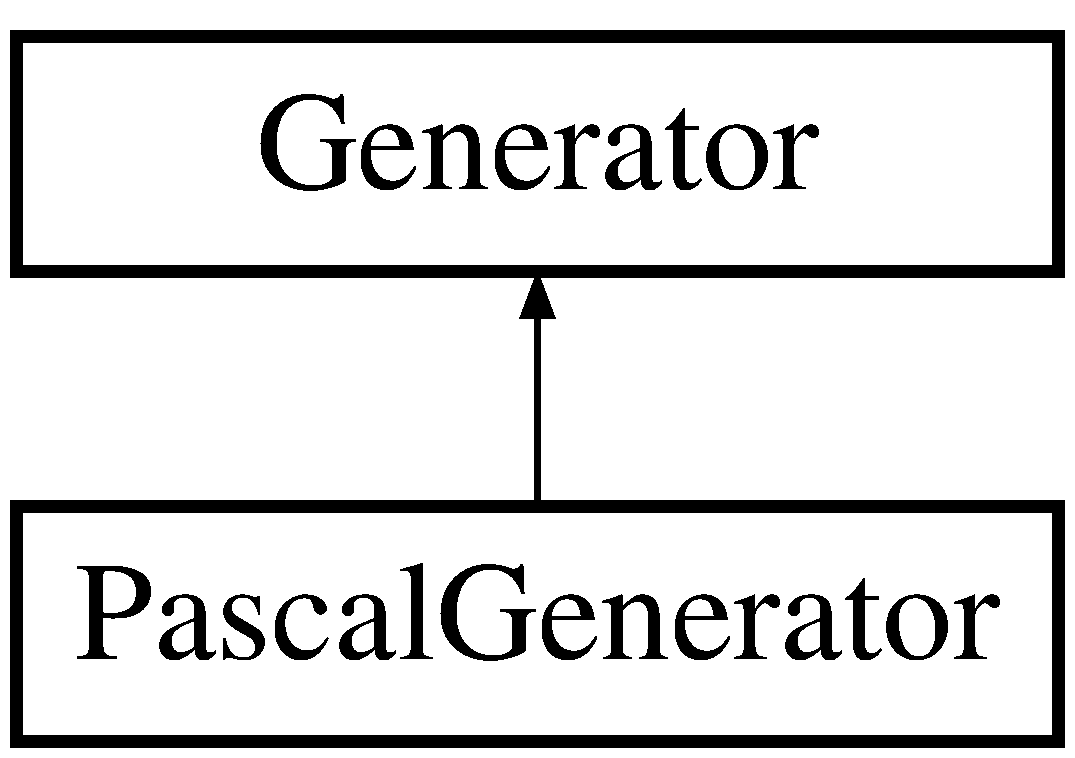
\includegraphics[height=2.000000cm]{classPascalGenerator}
\end{center}
\end{figure}
\subsection*{Public Member Functions}
\begin{DoxyCompactItemize}
\item 
virtual \hyperlink{classPascalGenerator_a24880843b5375abcf1a98178336ead78}{$\sim$\+Pascal\+Generator} ()
\item 
virtual void \hyperlink{classPascalGenerator_af0d2d3b1fbf63c8c4859b446541337c5}{generate} (\hyperlink{classN__Model}{N\+\_\+\+Model} \&m)
\item 
virtual std\+::string \hyperlink{classPascalGenerator_a45d98b0d7ee0cba9708bbce1cc6e81a8}{gen\+Interface} (\hyperlink{classN__Interface}{N\+\_\+\+Interface} $\ast$c)
\item 
virtual std\+::string \hyperlink{classPascalGenerator_a2518deea7c307b53d2f5569653772df4}{gen\+Field} (\hyperlink{classN__Field}{N\+\_\+\+Field} $\ast$f)
\item 
virtual std\+::string \hyperlink{classPascalGenerator_a676b9e2ca462c770d6eab2cd9150d078}{gen\+Method} (\hyperlink{classN__Method}{N\+\_\+\+Method} $\ast$m)
\item 
virtual std\+::string \hyperlink{classPascalGenerator_a588bf9c593871ccf52f5ab66d2b25258}{gen\+Method\+Header} (\hyperlink{classN__Method}{N\+\_\+\+Method} $\ast$m)
\item 
virtual std\+::string \hyperlink{classPascalGenerator_a4498120ec4549002fb575316f1f58257}{gen\+Parameter} (\hyperlink{classN__Param}{N\+\_\+\+Param} $\ast$p)
\item 
virtual std\+::string \hyperlink{classPascalGenerator_ae8bf162efb54e857c9a61bf9aae5f6e4}{gen\+Class} (\hyperlink{classN__Class}{N\+\_\+\+Class} $\ast$c)
\end{DoxyCompactItemize}
\subsection*{Protected Member Functions}
\begin{DoxyCompactItemize}
\item 
\hyperlink{classPascalGenerator_a83867974bbd27be21c906ea26a0a0524}{Pascal\+Generator} (std\+::ostream \&os)
\end{DoxyCompactItemize}
\subsection*{Friends}
\begin{DoxyCompactItemize}
\item 
class \hyperlink{classPascalGenerator_a366b7823e659ab78d952a7d79662a4d6}{Generator}
\end{DoxyCompactItemize}
\subsection*{Additional Inherited Members}


\subsection{Detailed Description}
Генератор кода на Pascal 

\subsection{Constructor \& Destructor Documentation}
\hypertarget{classPascalGenerator_a83867974bbd27be21c906ea26a0a0524}{}\index{Pascal\+Generator@{Pascal\+Generator}!Pascal\+Generator@{Pascal\+Generator}}
\index{Pascal\+Generator@{Pascal\+Generator}!Pascal\+Generator@{Pascal\+Generator}}
\subsubsection[{Pascal\+Generator}]{\setlength{\rightskip}{0pt plus 5cm}Pascal\+Generator\+::\+Pascal\+Generator (
\begin{DoxyParamCaption}
\item[{std\+::ostream \&}]{os}
\end{DoxyParamCaption}
)\hspace{0.3cm}{\ttfamily [inline]}, {\ttfamily [protected]}}\label{classPascalGenerator_a83867974bbd27be21c906ea26a0a0524}
\hypertarget{classPascalGenerator_a24880843b5375abcf1a98178336ead78}{}\index{Pascal\+Generator@{Pascal\+Generator}!````~Pascal\+Generator@{$\sim$\+Pascal\+Generator}}
\index{````~Pascal\+Generator@{$\sim$\+Pascal\+Generator}!Pascal\+Generator@{Pascal\+Generator}}
\subsubsection[{$\sim$\+Pascal\+Generator}]{\setlength{\rightskip}{0pt plus 5cm}virtual Pascal\+Generator\+::$\sim$\+Pascal\+Generator (
\begin{DoxyParamCaption}
{}
\end{DoxyParamCaption}
)\hspace{0.3cm}{\ttfamily [inline]}, {\ttfamily [virtual]}}\label{classPascalGenerator_a24880843b5375abcf1a98178336ead78}


\subsection{Member Function Documentation}
\hypertarget{classPascalGenerator_ae8bf162efb54e857c9a61bf9aae5f6e4}{}\index{Pascal\+Generator@{Pascal\+Generator}!gen\+Class@{gen\+Class}}
\index{gen\+Class@{gen\+Class}!Pascal\+Generator@{Pascal\+Generator}}
\subsubsection[{gen\+Class}]{\setlength{\rightskip}{0pt plus 5cm}std\+::string Pascal\+Generator\+::gen\+Class (
\begin{DoxyParamCaption}
\item[{{\bf N\+\_\+\+Class} $\ast$}]{c}
\end{DoxyParamCaption}
)\hspace{0.3cm}{\ttfamily [virtual]}}\label{classPascalGenerator_ae8bf162efb54e857c9a61bf9aae5f6e4}
Генератор шаблона класса 
\begin{DoxyParams}{Parameters}
{\em c} & -\/ класс, для которого необходимо сгенерировать шаблон \\
\hline
\end{DoxyParams}
\begin{DoxyReturn}{Returns}
Сгенерированный шаблон 
\end{DoxyReturn}


Implements \hyperlink{classGenerator_afac361fceae302fb09e8170d097415d4}{Generator}.

\hypertarget{classPascalGenerator_af0d2d3b1fbf63c8c4859b446541337c5}{}\index{Pascal\+Generator@{Pascal\+Generator}!generate@{generate}}
\index{generate@{generate}!Pascal\+Generator@{Pascal\+Generator}}
\subsubsection[{generate}]{\setlength{\rightskip}{0pt plus 5cm}void Pascal\+Generator\+::generate (
\begin{DoxyParamCaption}
\item[{{\bf N\+\_\+\+Model} \&}]{m}
\end{DoxyParamCaption}
)\hspace{0.3cm}{\ttfamily [virtual]}}\label{classPascalGenerator_af0d2d3b1fbf63c8c4859b446541337c5}
Генератор шаблона модели 
\begin{DoxyParams}{Parameters}
{\em m} & -\/ модель, для которой необходимо сгенерировать шаблон \\
\hline
\end{DoxyParams}


Implements \hyperlink{classGenerator_a518161ca79e68d733687f8e2985abd16}{Generator}.

\hypertarget{classPascalGenerator_a2518deea7c307b53d2f5569653772df4}{}\index{Pascal\+Generator@{Pascal\+Generator}!gen\+Field@{gen\+Field}}
\index{gen\+Field@{gen\+Field}!Pascal\+Generator@{Pascal\+Generator}}
\subsubsection[{gen\+Field}]{\setlength{\rightskip}{0pt plus 5cm}std\+::string Pascal\+Generator\+::gen\+Field (
\begin{DoxyParamCaption}
\item[{{\bf N\+\_\+\+Field} $\ast$}]{f}
\end{DoxyParamCaption}
)\hspace{0.3cm}{\ttfamily [virtual]}}\label{classPascalGenerator_a2518deea7c307b53d2f5569653772df4}
Генератор шаблона поля класса 
\begin{DoxyParams}{Parameters}
{\em f} & -\/ поле, для которого необходимо сгенерировать шаблон \\
\hline
\end{DoxyParams}
\begin{DoxyReturn}{Returns}
Сгенерированный шаблон 
\end{DoxyReturn}


Implements \hyperlink{classGenerator_aa2871c303fba42abd61a7ed997d23416}{Generator}.

\hypertarget{classPascalGenerator_a45d98b0d7ee0cba9708bbce1cc6e81a8}{}\index{Pascal\+Generator@{Pascal\+Generator}!gen\+Interface@{gen\+Interface}}
\index{gen\+Interface@{gen\+Interface}!Pascal\+Generator@{Pascal\+Generator}}
\subsubsection[{gen\+Interface}]{\setlength{\rightskip}{0pt plus 5cm}std\+::string Pascal\+Generator\+::gen\+Interface (
\begin{DoxyParamCaption}
\item[{{\bf N\+\_\+\+Interface} $\ast$}]{c}
\end{DoxyParamCaption}
)\hspace{0.3cm}{\ttfamily [virtual]}}\label{classPascalGenerator_a45d98b0d7ee0cba9708bbce1cc6e81a8}
Генератор шаблона интерфейса 
\begin{DoxyParams}{Parameters}
{\em c} & -\/ интерфейс, для которого необходимо сгенерировать шаблон \\
\hline
\end{DoxyParams}
\begin{DoxyReturn}{Returns}
Сгенерированный шаблон 
\end{DoxyReturn}


Implements \hyperlink{classGenerator_ad0f09fcc0e99e78e04f8c202cd0ce881}{Generator}.

\hypertarget{classPascalGenerator_a676b9e2ca462c770d6eab2cd9150d078}{}\index{Pascal\+Generator@{Pascal\+Generator}!gen\+Method@{gen\+Method}}
\index{gen\+Method@{gen\+Method}!Pascal\+Generator@{Pascal\+Generator}}
\subsubsection[{gen\+Method}]{\setlength{\rightskip}{0pt plus 5cm}std\+::string Pascal\+Generator\+::gen\+Method (
\begin{DoxyParamCaption}
\item[{{\bf N\+\_\+\+Method} $\ast$}]{m}
\end{DoxyParamCaption}
)\hspace{0.3cm}{\ttfamily [virtual]}}\label{classPascalGenerator_a676b9e2ca462c770d6eab2cd9150d078}
Генератор шаблона метода 
\begin{DoxyParams}{Parameters}
{\em m} & -\/ метод, для которого необходимо сгенерировать шаблон \\
\hline
\end{DoxyParams}
\begin{DoxyReturn}{Returns}
Сгенерированный шаблон 
\end{DoxyReturn}


Implements \hyperlink{classGenerator_a2b09ae359674038af5286fbd03d83c41}{Generator}.

\hypertarget{classPascalGenerator_a588bf9c593871ccf52f5ab66d2b25258}{}\index{Pascal\+Generator@{Pascal\+Generator}!gen\+Method\+Header@{gen\+Method\+Header}}
\index{gen\+Method\+Header@{gen\+Method\+Header}!Pascal\+Generator@{Pascal\+Generator}}
\subsubsection[{gen\+Method\+Header}]{\setlength{\rightskip}{0pt plus 5cm}std\+::string Pascal\+Generator\+::gen\+Method\+Header (
\begin{DoxyParamCaption}
\item[{{\bf N\+\_\+\+Method} $\ast$}]{m}
\end{DoxyParamCaption}
)\hspace{0.3cm}{\ttfamily [virtual]}}\label{classPascalGenerator_a588bf9c593871ccf52f5ab66d2b25258}
Генератор шаблона заголовка метода 
\begin{DoxyParams}{Parameters}
{\em m} & -\/ метод, для которого необходимо сгенерировать шаблон \\
\hline
\end{DoxyParams}
\begin{DoxyReturn}{Returns}
Сгенерированный шаблон 
\end{DoxyReturn}


Implements \hyperlink{classGenerator_aede7f5343c5bcd88b5fc8bfe51d17bce}{Generator}.

\hypertarget{classPascalGenerator_a4498120ec4549002fb575316f1f58257}{}\index{Pascal\+Generator@{Pascal\+Generator}!gen\+Parameter@{gen\+Parameter}}
\index{gen\+Parameter@{gen\+Parameter}!Pascal\+Generator@{Pascal\+Generator}}
\subsubsection[{gen\+Parameter}]{\setlength{\rightskip}{0pt plus 5cm}std\+::string Pascal\+Generator\+::gen\+Parameter (
\begin{DoxyParamCaption}
\item[{{\bf N\+\_\+\+Param} $\ast$}]{p}
\end{DoxyParamCaption}
)\hspace{0.3cm}{\ttfamily [virtual]}}\label{classPascalGenerator_a4498120ec4549002fb575316f1f58257}
Генератор шаблона параметра метода 
\begin{DoxyParams}{Parameters}
{\em p} & -\/ параметр, для которого необходимо сгенерировать шаблон \\
\hline
\end{DoxyParams}
\begin{DoxyReturn}{Returns}
Сгенерированный шаблон 
\end{DoxyReturn}


Implements \hyperlink{classGenerator_ac9871b3d5874cb81a98a3e5eb3b703e2}{Generator}.



\subsection{Friends And Related Function Documentation}
\hypertarget{classPascalGenerator_a366b7823e659ab78d952a7d79662a4d6}{}\index{Pascal\+Generator@{Pascal\+Generator}!Generator@{Generator}}
\index{Generator@{Generator}!Pascal\+Generator@{Pascal\+Generator}}
\subsubsection[{Generator}]{\setlength{\rightskip}{0pt plus 5cm}friend class {\bf Generator}\hspace{0.3cm}{\ttfamily [friend]}}\label{classPascalGenerator_a366b7823e659ab78d952a7d79662a4d6}


The documentation for this class was generated from the following files\+:\begin{DoxyCompactItemize}
\item 
\hyperlink{ast_8h}{ast.\+h}\item 
\hyperlink{ast_8cpp}{ast.\+cpp}\end{DoxyCompactItemize}

\hypertarget{structyy__buffer__state}{}\section{yy\+\_\+buffer\+\_\+state Struct Reference}
\label{structyy__buffer__state}\index{yy\+\_\+buffer\+\_\+state@{yy\+\_\+buffer\+\_\+state}}
\subsection*{Public Attributes}
\begin{DoxyCompactItemize}
\item 
F\+I\+L\+E $\ast$ \hyperlink{structyy__buffer__state_a4843d1422e3276b636d475a3095bd948}{yy\+\_\+input\+\_\+file}
\item 
char $\ast$ \hyperlink{structyy__buffer__state_ad7b8df8d8a4688e57b0b8d3ca75adc85}{yy\+\_\+ch\+\_\+buf}
\item 
char $\ast$ \hyperlink{structyy__buffer__state_a58aa927f098b99d99e75da80f9b681ef}{yy\+\_\+buf\+\_\+pos}
\item 
\hyperlink{lex_8yy_8c_ad557845057f187eec4be07e2717d2afa}{yy\+\_\+size\+\_\+t} \hyperlink{structyy__buffer__state_a48302f5f3477a9c78bbddf56d356ef54}{yy\+\_\+buf\+\_\+size}
\item 
\hyperlink{lex_8yy_8c_ad557845057f187eec4be07e2717d2afa}{yy\+\_\+size\+\_\+t} \hyperlink{structyy__buffer__state_afcc44872643f513e79b43c2b1f334a67}{yy\+\_\+n\+\_\+chars}
\item 
int \hyperlink{structyy__buffer__state_a80ce2431c70dc4f89ced487f18449465}{yy\+\_\+is\+\_\+our\+\_\+buffer}
\item 
int \hyperlink{structyy__buffer__state_abf5c70eea75581b58c0ee7bd31b14490}{yy\+\_\+is\+\_\+interactive}
\item 
int \hyperlink{structyy__buffer__state_a9d60c60af6e1a6f69de16871fd64f85f}{yy\+\_\+at\+\_\+bol}
\item 
int \hyperlink{structyy__buffer__state_a818e94bc9c766e683c60df1e9fd01199}{yy\+\_\+bs\+\_\+lineno}
\item 
int \hyperlink{structyy__buffer__state_a10c4fcd8be759e6bf11e6d3e8cdb0307}{yy\+\_\+bs\+\_\+column}
\item 
int \hyperlink{structyy__buffer__state_a63d2afbb1d79a3fc63df9e12626f827d}{yy\+\_\+fill\+\_\+buffer}
\item 
int \hyperlink{structyy__buffer__state_a70fd925d37a2f0454fbd0def675d106c}{yy\+\_\+buffer\+\_\+status}
\end{DoxyCompactItemize}


\subsection{Member Data Documentation}
\hypertarget{structyy__buffer__state_a9d60c60af6e1a6f69de16871fd64f85f}{}\index{yy\+\_\+buffer\+\_\+state@{yy\+\_\+buffer\+\_\+state}!yy\+\_\+at\+\_\+bol@{yy\+\_\+at\+\_\+bol}}
\index{yy\+\_\+at\+\_\+bol@{yy\+\_\+at\+\_\+bol}!yy\+\_\+buffer\+\_\+state@{yy\+\_\+buffer\+\_\+state}}
\subsubsection[{yy\+\_\+at\+\_\+bol}]{\setlength{\rightskip}{0pt plus 5cm}int yy\+\_\+buffer\+\_\+state\+::yy\+\_\+at\+\_\+bol}\label{structyy__buffer__state_a9d60c60af6e1a6f69de16871fd64f85f}
\hypertarget{structyy__buffer__state_a10c4fcd8be759e6bf11e6d3e8cdb0307}{}\index{yy\+\_\+buffer\+\_\+state@{yy\+\_\+buffer\+\_\+state}!yy\+\_\+bs\+\_\+column@{yy\+\_\+bs\+\_\+column}}
\index{yy\+\_\+bs\+\_\+column@{yy\+\_\+bs\+\_\+column}!yy\+\_\+buffer\+\_\+state@{yy\+\_\+buffer\+\_\+state}}
\subsubsection[{yy\+\_\+bs\+\_\+column}]{\setlength{\rightskip}{0pt plus 5cm}int yy\+\_\+buffer\+\_\+state\+::yy\+\_\+bs\+\_\+column}\label{structyy__buffer__state_a10c4fcd8be759e6bf11e6d3e8cdb0307}
The column count. \hypertarget{structyy__buffer__state_a818e94bc9c766e683c60df1e9fd01199}{}\index{yy\+\_\+buffer\+\_\+state@{yy\+\_\+buffer\+\_\+state}!yy\+\_\+bs\+\_\+lineno@{yy\+\_\+bs\+\_\+lineno}}
\index{yy\+\_\+bs\+\_\+lineno@{yy\+\_\+bs\+\_\+lineno}!yy\+\_\+buffer\+\_\+state@{yy\+\_\+buffer\+\_\+state}}
\subsubsection[{yy\+\_\+bs\+\_\+lineno}]{\setlength{\rightskip}{0pt plus 5cm}int yy\+\_\+buffer\+\_\+state\+::yy\+\_\+bs\+\_\+lineno}\label{structyy__buffer__state_a818e94bc9c766e683c60df1e9fd01199}
The line count. \hypertarget{structyy__buffer__state_a58aa927f098b99d99e75da80f9b681ef}{}\index{yy\+\_\+buffer\+\_\+state@{yy\+\_\+buffer\+\_\+state}!yy\+\_\+buf\+\_\+pos@{yy\+\_\+buf\+\_\+pos}}
\index{yy\+\_\+buf\+\_\+pos@{yy\+\_\+buf\+\_\+pos}!yy\+\_\+buffer\+\_\+state@{yy\+\_\+buffer\+\_\+state}}
\subsubsection[{yy\+\_\+buf\+\_\+pos}]{\setlength{\rightskip}{0pt plus 5cm}char$\ast$ yy\+\_\+buffer\+\_\+state\+::yy\+\_\+buf\+\_\+pos}\label{structyy__buffer__state_a58aa927f098b99d99e75da80f9b681ef}
\hypertarget{structyy__buffer__state_a48302f5f3477a9c78bbddf56d356ef54}{}\index{yy\+\_\+buffer\+\_\+state@{yy\+\_\+buffer\+\_\+state}!yy\+\_\+buf\+\_\+size@{yy\+\_\+buf\+\_\+size}}
\index{yy\+\_\+buf\+\_\+size@{yy\+\_\+buf\+\_\+size}!yy\+\_\+buffer\+\_\+state@{yy\+\_\+buffer\+\_\+state}}
\subsubsection[{yy\+\_\+buf\+\_\+size}]{\setlength{\rightskip}{0pt plus 5cm}{\bf yy\+\_\+size\+\_\+t} yy\+\_\+buffer\+\_\+state\+::yy\+\_\+buf\+\_\+size}\label{structyy__buffer__state_a48302f5f3477a9c78bbddf56d356ef54}
\hypertarget{structyy__buffer__state_a70fd925d37a2f0454fbd0def675d106c}{}\index{yy\+\_\+buffer\+\_\+state@{yy\+\_\+buffer\+\_\+state}!yy\+\_\+buffer\+\_\+status@{yy\+\_\+buffer\+\_\+status}}
\index{yy\+\_\+buffer\+\_\+status@{yy\+\_\+buffer\+\_\+status}!yy\+\_\+buffer\+\_\+state@{yy\+\_\+buffer\+\_\+state}}
\subsubsection[{yy\+\_\+buffer\+\_\+status}]{\setlength{\rightskip}{0pt plus 5cm}int yy\+\_\+buffer\+\_\+state\+::yy\+\_\+buffer\+\_\+status}\label{structyy__buffer__state_a70fd925d37a2f0454fbd0def675d106c}
\hypertarget{structyy__buffer__state_ad7b8df8d8a4688e57b0b8d3ca75adc85}{}\index{yy\+\_\+buffer\+\_\+state@{yy\+\_\+buffer\+\_\+state}!yy\+\_\+ch\+\_\+buf@{yy\+\_\+ch\+\_\+buf}}
\index{yy\+\_\+ch\+\_\+buf@{yy\+\_\+ch\+\_\+buf}!yy\+\_\+buffer\+\_\+state@{yy\+\_\+buffer\+\_\+state}}
\subsubsection[{yy\+\_\+ch\+\_\+buf}]{\setlength{\rightskip}{0pt plus 5cm}char$\ast$ yy\+\_\+buffer\+\_\+state\+::yy\+\_\+ch\+\_\+buf}\label{structyy__buffer__state_ad7b8df8d8a4688e57b0b8d3ca75adc85}
\hypertarget{structyy__buffer__state_a63d2afbb1d79a3fc63df9e12626f827d}{}\index{yy\+\_\+buffer\+\_\+state@{yy\+\_\+buffer\+\_\+state}!yy\+\_\+fill\+\_\+buffer@{yy\+\_\+fill\+\_\+buffer}}
\index{yy\+\_\+fill\+\_\+buffer@{yy\+\_\+fill\+\_\+buffer}!yy\+\_\+buffer\+\_\+state@{yy\+\_\+buffer\+\_\+state}}
\subsubsection[{yy\+\_\+fill\+\_\+buffer}]{\setlength{\rightskip}{0pt plus 5cm}int yy\+\_\+buffer\+\_\+state\+::yy\+\_\+fill\+\_\+buffer}\label{structyy__buffer__state_a63d2afbb1d79a3fc63df9e12626f827d}
\hypertarget{structyy__buffer__state_a4843d1422e3276b636d475a3095bd948}{}\index{yy\+\_\+buffer\+\_\+state@{yy\+\_\+buffer\+\_\+state}!yy\+\_\+input\+\_\+file@{yy\+\_\+input\+\_\+file}}
\index{yy\+\_\+input\+\_\+file@{yy\+\_\+input\+\_\+file}!yy\+\_\+buffer\+\_\+state@{yy\+\_\+buffer\+\_\+state}}
\subsubsection[{yy\+\_\+input\+\_\+file}]{\setlength{\rightskip}{0pt plus 5cm}F\+I\+L\+E$\ast$ yy\+\_\+buffer\+\_\+state\+::yy\+\_\+input\+\_\+file}\label{structyy__buffer__state_a4843d1422e3276b636d475a3095bd948}
\hypertarget{structyy__buffer__state_abf5c70eea75581b58c0ee7bd31b14490}{}\index{yy\+\_\+buffer\+\_\+state@{yy\+\_\+buffer\+\_\+state}!yy\+\_\+is\+\_\+interactive@{yy\+\_\+is\+\_\+interactive}}
\index{yy\+\_\+is\+\_\+interactive@{yy\+\_\+is\+\_\+interactive}!yy\+\_\+buffer\+\_\+state@{yy\+\_\+buffer\+\_\+state}}
\subsubsection[{yy\+\_\+is\+\_\+interactive}]{\setlength{\rightskip}{0pt plus 5cm}int yy\+\_\+buffer\+\_\+state\+::yy\+\_\+is\+\_\+interactive}\label{structyy__buffer__state_abf5c70eea75581b58c0ee7bd31b14490}
\hypertarget{structyy__buffer__state_a80ce2431c70dc4f89ced487f18449465}{}\index{yy\+\_\+buffer\+\_\+state@{yy\+\_\+buffer\+\_\+state}!yy\+\_\+is\+\_\+our\+\_\+buffer@{yy\+\_\+is\+\_\+our\+\_\+buffer}}
\index{yy\+\_\+is\+\_\+our\+\_\+buffer@{yy\+\_\+is\+\_\+our\+\_\+buffer}!yy\+\_\+buffer\+\_\+state@{yy\+\_\+buffer\+\_\+state}}
\subsubsection[{yy\+\_\+is\+\_\+our\+\_\+buffer}]{\setlength{\rightskip}{0pt plus 5cm}int yy\+\_\+buffer\+\_\+state\+::yy\+\_\+is\+\_\+our\+\_\+buffer}\label{structyy__buffer__state_a80ce2431c70dc4f89ced487f18449465}
\hypertarget{structyy__buffer__state_afcc44872643f513e79b43c2b1f334a67}{}\index{yy\+\_\+buffer\+\_\+state@{yy\+\_\+buffer\+\_\+state}!yy\+\_\+n\+\_\+chars@{yy\+\_\+n\+\_\+chars}}
\index{yy\+\_\+n\+\_\+chars@{yy\+\_\+n\+\_\+chars}!yy\+\_\+buffer\+\_\+state@{yy\+\_\+buffer\+\_\+state}}
\subsubsection[{yy\+\_\+n\+\_\+chars}]{\setlength{\rightskip}{0pt plus 5cm}{\bf yy\+\_\+size\+\_\+t} yy\+\_\+buffer\+\_\+state\+::yy\+\_\+n\+\_\+chars}\label{structyy__buffer__state_afcc44872643f513e79b43c2b1f334a67}


The documentation for this struct was generated from the following file\+:\begin{DoxyCompactItemize}
\item 
\hyperlink{lex_8yy_8c}{lex.\+yy.\+c}\end{DoxyCompactItemize}

\hypertarget{structyy__trans__info}{}\section{yy\+\_\+trans\+\_\+info Struct Reference}
\label{structyy__trans__info}\index{yy\+\_\+trans\+\_\+info@{yy\+\_\+trans\+\_\+info}}
\subsection*{Public Attributes}
\begin{DoxyCompactItemize}
\item 
\hyperlink{lex_8yy_8c_a838ce943cf44ef7769480714fc6c3ba9}{flex\+\_\+int32\+\_\+t} \hyperlink{structyy__trans__info_a5c9f61e770deef50bd4e697310342fe9}{yy\+\_\+verify}
\item 
\hyperlink{lex_8yy_8c_a838ce943cf44ef7769480714fc6c3ba9}{flex\+\_\+int32\+\_\+t} \hyperlink{structyy__trans__info_ae0715250c2bef261e596e77e0030f13e}{yy\+\_\+nxt}
\end{DoxyCompactItemize}


\subsection{Member Data Documentation}
\hypertarget{structyy__trans__info_ae0715250c2bef261e596e77e0030f13e}{}\index{yy\+\_\+trans\+\_\+info@{yy\+\_\+trans\+\_\+info}!yy\+\_\+nxt@{yy\+\_\+nxt}}
\index{yy\+\_\+nxt@{yy\+\_\+nxt}!yy\+\_\+trans\+\_\+info@{yy\+\_\+trans\+\_\+info}}
\subsubsection[{yy\+\_\+nxt}]{\setlength{\rightskip}{0pt plus 5cm}{\bf flex\+\_\+int32\+\_\+t} yy\+\_\+trans\+\_\+info\+::yy\+\_\+nxt}\label{structyy__trans__info_ae0715250c2bef261e596e77e0030f13e}
\hypertarget{structyy__trans__info_a5c9f61e770deef50bd4e697310342fe9}{}\index{yy\+\_\+trans\+\_\+info@{yy\+\_\+trans\+\_\+info}!yy\+\_\+verify@{yy\+\_\+verify}}
\index{yy\+\_\+verify@{yy\+\_\+verify}!yy\+\_\+trans\+\_\+info@{yy\+\_\+trans\+\_\+info}}
\subsubsection[{yy\+\_\+verify}]{\setlength{\rightskip}{0pt plus 5cm}{\bf flex\+\_\+int32\+\_\+t} yy\+\_\+trans\+\_\+info\+::yy\+\_\+verify}\label{structyy__trans__info_a5c9f61e770deef50bd4e697310342fe9}


The documentation for this struct was generated from the following file\+:\begin{DoxyCompactItemize}
\item 
\hyperlink{lex_8yy_8c}{lex.\+yy.\+c}\end{DoxyCompactItemize}

\hypertarget{unionyyalloc}{}\section{yyalloc Union Reference}
\label{unionyyalloc}\index{yyalloc@{yyalloc}}
\subsection*{Public Attributes}
\begin{DoxyCompactItemize}
\item 
\hyperlink{parser_8cpp_ade5b97f0021a4f6c5922ead3744ab297}{yytype\+\_\+int16} \hyperlink{unionyyalloc_a4800e0520a89a4789afa7b5d82197e65}{yyss\+\_\+alloc}
\item 
\hyperlink{unionYYSTYPE}{Y\+Y\+S\+T\+Y\+P\+E} \hyperlink{unionyyalloc_a9326f4fdc6f737a929444427836d8928}{yyvs\+\_\+alloc}
\end{DoxyCompactItemize}


\subsection{Member Data Documentation}
\hypertarget{unionyyalloc_a4800e0520a89a4789afa7b5d82197e65}{}\index{yyalloc@{yyalloc}!yyss\+\_\+alloc@{yyss\+\_\+alloc}}
\index{yyss\+\_\+alloc@{yyss\+\_\+alloc}!yyalloc@{yyalloc}}
\subsubsection[{yyss\+\_\+alloc}]{\setlength{\rightskip}{0pt plus 5cm}{\bf yytype\+\_\+int16} yyalloc\+::yyss\+\_\+alloc}\label{unionyyalloc_a4800e0520a89a4789afa7b5d82197e65}
\hypertarget{unionyyalloc_a9326f4fdc6f737a929444427836d8928}{}\index{yyalloc@{yyalloc}!yyvs\+\_\+alloc@{yyvs\+\_\+alloc}}
\index{yyvs\+\_\+alloc@{yyvs\+\_\+alloc}!yyalloc@{yyalloc}}
\subsubsection[{yyvs\+\_\+alloc}]{\setlength{\rightskip}{0pt plus 5cm}{\bf Y\+Y\+S\+T\+Y\+P\+E} yyalloc\+::yyvs\+\_\+alloc}\label{unionyyalloc_a9326f4fdc6f737a929444427836d8928}


The documentation for this union was generated from the following file\+:\begin{DoxyCompactItemize}
\item 
\hyperlink{parser_8cpp}{parser.\+cpp}\end{DoxyCompactItemize}

\hypertarget{unionYYSTYPE}{}\section{Y\+Y\+S\+T\+Y\+P\+E Union Reference}
\label{unionYYSTYPE}\index{Y\+Y\+S\+T\+Y\+P\+E@{Y\+Y\+S\+T\+Y\+P\+E}}


{\ttfamily \#include $<$parser.\+hpp$>$}

\subsection*{Public Attributes}
\begin{DoxyCompactItemize}
\item 
std\+::string $\ast$ \hyperlink{unionYYSTYPE_a4bd606f3c9cec57ee4ba48957509b3f8}{string}
\item 
int \hyperlink{unionYYSTYPE_a01b79e2c4a8e5ec028cca4892559e802}{token}
\item 
int \hyperlink{unionYYSTYPE_acfe61c5751a9282c4ea0d9b345de371b}{value}
\item 
\hyperlink{classN__Model}{N\+\_\+\+Model} $\ast$ \hyperlink{unionYYSTYPE_aa8af89ba8550850302ca1099549db8a9}{model}
\item 
std\+::vector$<$ \hyperlink{classN__ModelMember}{N\+\_\+\+Model\+Member} $\ast$ $>$ $\ast$ \hyperlink{unionYYSTYPE_a504a37d0452901592deb404b4dde2515}{model\+\_\+member\+\_\+list}
\item 
\hyperlink{classN__ModelMember}{N\+\_\+\+Model\+Member} $\ast$ \hyperlink{unionYYSTYPE_a02056d0aa2eaaccc40409baafd79168d}{model\+\_\+member}
\item 
\hyperlink{classN__ModelOption}{N\+\_\+\+Model\+Option} $\ast$ \hyperlink{unionYYSTYPE_af1e284dc24f28c72ea7e0ed867f34e04}{model\+\_\+option}
\item 
int \hyperlink{unionYYSTYPE_a341e3656f8fb6711150f09f741dedd6c}{model\+\_\+import}
\item 
\hyperlink{classN__Type}{N\+\_\+\+Type} $\ast$ \hyperlink{unionYYSTYPE_a2262e4fdf23475305af071cf2dce24f3}{model\+\_\+type}
\item 
\hyperlink{classN__Interface}{N\+\_\+\+Interface} $\ast$ \hyperlink{unionYYSTYPE_a29fba859c02418376ff3bfd6b9750c35}{model\+\_\+interface}
\item 
\hyperlink{classN__Class}{N\+\_\+\+Class} $\ast$ \hyperlink{unionYYSTYPE_af7b370bf86459f13b2ecc2c0732ecaf4}{model\+\_\+class}
\item 
std\+::vector$<$ std\+::string $>$ $\ast$ \hyperlink{unionYYSTYPE_aca50ce01e3307959b0acf7740f490170}{string\+\_\+list}
\item 
\hyperlink{classN__ClassMember}{N\+\_\+\+Class\+Member} $\ast$ \hyperlink{unionYYSTYPE_aab8ffd3479e64f4f952a8b229c4c7c5a}{model\+\_\+class\+\_\+member}
\item 
std\+::vector$<$ \hyperlink{classN__ClassMember}{N\+\_\+\+Class\+Member} $\ast$ $>$ $\ast$ \hyperlink{unionYYSTYPE_a1bf423ad9f460d4e74c00bb8670eaae8}{model\+\_\+class\+\_\+member\+\_\+list}
\item 
\hyperlink{classN__Method}{N\+\_\+\+Method} $\ast$ \hyperlink{unionYYSTYPE_a942a640237407a4473209637bb4e8875}{model\+\_\+method}
\item 
\hyperlink{classN__Field}{N\+\_\+\+Field} $\ast$ \hyperlink{unionYYSTYPE_af2e876cf0d3eea8c18d7a91f3639ad8b}{model\+\_\+field}
\item 
\hyperlink{ast_8h_a8cf536792064de0e4fc620bc6f1dc90e}{Member\+Visibility} \hyperlink{unionYYSTYPE_ab17b1393dae8de54663649a094da13ed}{model\+\_\+visibility}
\item 
\hyperlink{structMethodTypeInfo}{Method\+Type\+Info} \hyperlink{unionYYSTYPE_ad9e7689680a21064dcf7e957194c83fc}{model\+\_\+method\+\_\+type}
\item 
bool \hyperlink{unionYYSTYPE_a19de40e9bab839895eb0b143194367dc}{model\+\_\+method\+\_\+is\+\_\+static}
\item 
\hyperlink{ast_8h_a6e3e364b8758e35526082aefa26d3596}{Stereotype} \hyperlink{unionYYSTYPE_af24face112bb5754e94b4fd2b0c666c1}{model\+\_\+stereotype}
\item 
std\+::vector$<$ \hyperlink{classN__Exception}{N\+\_\+\+Exception} $\ast$ $>$ $\ast$ \hyperlink{unionYYSTYPE_a04dfac3d4b5c7515b14c1b8971eed3d4}{model\+\_\+exception\+\_\+list}
\item 
\hyperlink{classN__Exception}{N\+\_\+\+Exception} $\ast$ \hyperlink{unionYYSTYPE_a713476977a927a84863073eb5025ed91}{model\+\_\+exception}
\item 
\hyperlink{classN__Param}{N\+\_\+\+Param} $\ast$ \hyperlink{unionYYSTYPE_ae48a50d0b50d47f49c22d92a1d648d64}{model\+\_\+param}
\item 
std\+::vector$<$ \hyperlink{classN__Param}{N\+\_\+\+Param} $\ast$ $>$ $\ast$ \hyperlink{unionYYSTYPE_a6eb4e2ebafb8f2fbb80f8d8cf51d3bae}{model\+\_\+param\+\_\+list}
\item 
\hyperlink{ast_8h_af1bb1892f9e576501ff47410367569a7}{Param\+Direction} \hyperlink{unionYYSTYPE_a000fd2ef5a9eeffa92a050ae325a170d}{model\+\_\+param\+\_\+direction}
\end{DoxyCompactItemize}


\subsection{Member Data Documentation}
\hypertarget{unionYYSTYPE_aa8af89ba8550850302ca1099549db8a9}{}\index{Y\+Y\+S\+T\+Y\+P\+E@{Y\+Y\+S\+T\+Y\+P\+E}!model@{model}}
\index{model@{model}!Y\+Y\+S\+T\+Y\+P\+E@{Y\+Y\+S\+T\+Y\+P\+E}}
\subsubsection[{model}]{\setlength{\rightskip}{0pt plus 5cm}{\bf N\+\_\+\+Model}$\ast$ Y\+Y\+S\+T\+Y\+P\+E\+::model}\label{unionYYSTYPE_aa8af89ba8550850302ca1099549db8a9}
\hypertarget{unionYYSTYPE_af7b370bf86459f13b2ecc2c0732ecaf4}{}\index{Y\+Y\+S\+T\+Y\+P\+E@{Y\+Y\+S\+T\+Y\+P\+E}!model\+\_\+class@{model\+\_\+class}}
\index{model\+\_\+class@{model\+\_\+class}!Y\+Y\+S\+T\+Y\+P\+E@{Y\+Y\+S\+T\+Y\+P\+E}}
\subsubsection[{model\+\_\+class}]{\setlength{\rightskip}{0pt plus 5cm}{\bf N\+\_\+\+Class}$\ast$ Y\+Y\+S\+T\+Y\+P\+E\+::model\+\_\+class}\label{unionYYSTYPE_af7b370bf86459f13b2ecc2c0732ecaf4}
\hypertarget{unionYYSTYPE_aab8ffd3479e64f4f952a8b229c4c7c5a}{}\index{Y\+Y\+S\+T\+Y\+P\+E@{Y\+Y\+S\+T\+Y\+P\+E}!model\+\_\+class\+\_\+member@{model\+\_\+class\+\_\+member}}
\index{model\+\_\+class\+\_\+member@{model\+\_\+class\+\_\+member}!Y\+Y\+S\+T\+Y\+P\+E@{Y\+Y\+S\+T\+Y\+P\+E}}
\subsubsection[{model\+\_\+class\+\_\+member}]{\setlength{\rightskip}{0pt plus 5cm}{\bf N\+\_\+\+Class\+Member}$\ast$ Y\+Y\+S\+T\+Y\+P\+E\+::model\+\_\+class\+\_\+member}\label{unionYYSTYPE_aab8ffd3479e64f4f952a8b229c4c7c5a}
\hypertarget{unionYYSTYPE_a1bf423ad9f460d4e74c00bb8670eaae8}{}\index{Y\+Y\+S\+T\+Y\+P\+E@{Y\+Y\+S\+T\+Y\+P\+E}!model\+\_\+class\+\_\+member\+\_\+list@{model\+\_\+class\+\_\+member\+\_\+list}}
\index{model\+\_\+class\+\_\+member\+\_\+list@{model\+\_\+class\+\_\+member\+\_\+list}!Y\+Y\+S\+T\+Y\+P\+E@{Y\+Y\+S\+T\+Y\+P\+E}}
\subsubsection[{model\+\_\+class\+\_\+member\+\_\+list}]{\setlength{\rightskip}{0pt plus 5cm}std\+::vector$<${\bf N\+\_\+\+Class\+Member}$\ast$$>$$\ast$ Y\+Y\+S\+T\+Y\+P\+E\+::model\+\_\+class\+\_\+member\+\_\+list}\label{unionYYSTYPE_a1bf423ad9f460d4e74c00bb8670eaae8}
\hypertarget{unionYYSTYPE_a713476977a927a84863073eb5025ed91}{}\index{Y\+Y\+S\+T\+Y\+P\+E@{Y\+Y\+S\+T\+Y\+P\+E}!model\+\_\+exception@{model\+\_\+exception}}
\index{model\+\_\+exception@{model\+\_\+exception}!Y\+Y\+S\+T\+Y\+P\+E@{Y\+Y\+S\+T\+Y\+P\+E}}
\subsubsection[{model\+\_\+exception}]{\setlength{\rightskip}{0pt plus 5cm}{\bf N\+\_\+\+Exception}$\ast$ Y\+Y\+S\+T\+Y\+P\+E\+::model\+\_\+exception}\label{unionYYSTYPE_a713476977a927a84863073eb5025ed91}
\hypertarget{unionYYSTYPE_a04dfac3d4b5c7515b14c1b8971eed3d4}{}\index{Y\+Y\+S\+T\+Y\+P\+E@{Y\+Y\+S\+T\+Y\+P\+E}!model\+\_\+exception\+\_\+list@{model\+\_\+exception\+\_\+list}}
\index{model\+\_\+exception\+\_\+list@{model\+\_\+exception\+\_\+list}!Y\+Y\+S\+T\+Y\+P\+E@{Y\+Y\+S\+T\+Y\+P\+E}}
\subsubsection[{model\+\_\+exception\+\_\+list}]{\setlength{\rightskip}{0pt plus 5cm}std\+::vector$<${\bf N\+\_\+\+Exception}$\ast$$>$$\ast$ Y\+Y\+S\+T\+Y\+P\+E\+::model\+\_\+exception\+\_\+list}\label{unionYYSTYPE_a04dfac3d4b5c7515b14c1b8971eed3d4}
\hypertarget{unionYYSTYPE_af2e876cf0d3eea8c18d7a91f3639ad8b}{}\index{Y\+Y\+S\+T\+Y\+P\+E@{Y\+Y\+S\+T\+Y\+P\+E}!model\+\_\+field@{model\+\_\+field}}
\index{model\+\_\+field@{model\+\_\+field}!Y\+Y\+S\+T\+Y\+P\+E@{Y\+Y\+S\+T\+Y\+P\+E}}
\subsubsection[{model\+\_\+field}]{\setlength{\rightskip}{0pt plus 5cm}{\bf N\+\_\+\+Field}$\ast$ Y\+Y\+S\+T\+Y\+P\+E\+::model\+\_\+field}\label{unionYYSTYPE_af2e876cf0d3eea8c18d7a91f3639ad8b}
\hypertarget{unionYYSTYPE_a341e3656f8fb6711150f09f741dedd6c}{}\index{Y\+Y\+S\+T\+Y\+P\+E@{Y\+Y\+S\+T\+Y\+P\+E}!model\+\_\+import@{model\+\_\+import}}
\index{model\+\_\+import@{model\+\_\+import}!Y\+Y\+S\+T\+Y\+P\+E@{Y\+Y\+S\+T\+Y\+P\+E}}
\subsubsection[{model\+\_\+import}]{\setlength{\rightskip}{0pt plus 5cm}int Y\+Y\+S\+T\+Y\+P\+E\+::model\+\_\+import}\label{unionYYSTYPE_a341e3656f8fb6711150f09f741dedd6c}
\hypertarget{unionYYSTYPE_a29fba859c02418376ff3bfd6b9750c35}{}\index{Y\+Y\+S\+T\+Y\+P\+E@{Y\+Y\+S\+T\+Y\+P\+E}!model\+\_\+interface@{model\+\_\+interface}}
\index{model\+\_\+interface@{model\+\_\+interface}!Y\+Y\+S\+T\+Y\+P\+E@{Y\+Y\+S\+T\+Y\+P\+E}}
\subsubsection[{model\+\_\+interface}]{\setlength{\rightskip}{0pt plus 5cm}{\bf N\+\_\+\+Interface}$\ast$ Y\+Y\+S\+T\+Y\+P\+E\+::model\+\_\+interface}\label{unionYYSTYPE_a29fba859c02418376ff3bfd6b9750c35}
\hypertarget{unionYYSTYPE_a02056d0aa2eaaccc40409baafd79168d}{}\index{Y\+Y\+S\+T\+Y\+P\+E@{Y\+Y\+S\+T\+Y\+P\+E}!model\+\_\+member@{model\+\_\+member}}
\index{model\+\_\+member@{model\+\_\+member}!Y\+Y\+S\+T\+Y\+P\+E@{Y\+Y\+S\+T\+Y\+P\+E}}
\subsubsection[{model\+\_\+member}]{\setlength{\rightskip}{0pt plus 5cm}{\bf N\+\_\+\+Model\+Member}$\ast$ Y\+Y\+S\+T\+Y\+P\+E\+::model\+\_\+member}\label{unionYYSTYPE_a02056d0aa2eaaccc40409baafd79168d}
\hypertarget{unionYYSTYPE_a504a37d0452901592deb404b4dde2515}{}\index{Y\+Y\+S\+T\+Y\+P\+E@{Y\+Y\+S\+T\+Y\+P\+E}!model\+\_\+member\+\_\+list@{model\+\_\+member\+\_\+list}}
\index{model\+\_\+member\+\_\+list@{model\+\_\+member\+\_\+list}!Y\+Y\+S\+T\+Y\+P\+E@{Y\+Y\+S\+T\+Y\+P\+E}}
\subsubsection[{model\+\_\+member\+\_\+list}]{\setlength{\rightskip}{0pt plus 5cm}std\+::vector$<${\bf N\+\_\+\+Model\+Member}$\ast$$>$$\ast$ Y\+Y\+S\+T\+Y\+P\+E\+::model\+\_\+member\+\_\+list}\label{unionYYSTYPE_a504a37d0452901592deb404b4dde2515}
\hypertarget{unionYYSTYPE_a942a640237407a4473209637bb4e8875}{}\index{Y\+Y\+S\+T\+Y\+P\+E@{Y\+Y\+S\+T\+Y\+P\+E}!model\+\_\+method@{model\+\_\+method}}
\index{model\+\_\+method@{model\+\_\+method}!Y\+Y\+S\+T\+Y\+P\+E@{Y\+Y\+S\+T\+Y\+P\+E}}
\subsubsection[{model\+\_\+method}]{\setlength{\rightskip}{0pt plus 5cm}{\bf N\+\_\+\+Method}$\ast$ Y\+Y\+S\+T\+Y\+P\+E\+::model\+\_\+method}\label{unionYYSTYPE_a942a640237407a4473209637bb4e8875}
\hypertarget{unionYYSTYPE_a19de40e9bab839895eb0b143194367dc}{}\index{Y\+Y\+S\+T\+Y\+P\+E@{Y\+Y\+S\+T\+Y\+P\+E}!model\+\_\+method\+\_\+is\+\_\+static@{model\+\_\+method\+\_\+is\+\_\+static}}
\index{model\+\_\+method\+\_\+is\+\_\+static@{model\+\_\+method\+\_\+is\+\_\+static}!Y\+Y\+S\+T\+Y\+P\+E@{Y\+Y\+S\+T\+Y\+P\+E}}
\subsubsection[{model\+\_\+method\+\_\+is\+\_\+static}]{\setlength{\rightskip}{0pt plus 5cm}bool Y\+Y\+S\+T\+Y\+P\+E\+::model\+\_\+method\+\_\+is\+\_\+static}\label{unionYYSTYPE_a19de40e9bab839895eb0b143194367dc}
\hypertarget{unionYYSTYPE_ad9e7689680a21064dcf7e957194c83fc}{}\index{Y\+Y\+S\+T\+Y\+P\+E@{Y\+Y\+S\+T\+Y\+P\+E}!model\+\_\+method\+\_\+type@{model\+\_\+method\+\_\+type}}
\index{model\+\_\+method\+\_\+type@{model\+\_\+method\+\_\+type}!Y\+Y\+S\+T\+Y\+P\+E@{Y\+Y\+S\+T\+Y\+P\+E}}
\subsubsection[{model\+\_\+method\+\_\+type}]{\setlength{\rightskip}{0pt plus 5cm}{\bf Method\+Type\+Info} Y\+Y\+S\+T\+Y\+P\+E\+::model\+\_\+method\+\_\+type}\label{unionYYSTYPE_ad9e7689680a21064dcf7e957194c83fc}
\hypertarget{unionYYSTYPE_af1e284dc24f28c72ea7e0ed867f34e04}{}\index{Y\+Y\+S\+T\+Y\+P\+E@{Y\+Y\+S\+T\+Y\+P\+E}!model\+\_\+option@{model\+\_\+option}}
\index{model\+\_\+option@{model\+\_\+option}!Y\+Y\+S\+T\+Y\+P\+E@{Y\+Y\+S\+T\+Y\+P\+E}}
\subsubsection[{model\+\_\+option}]{\setlength{\rightskip}{0pt plus 5cm}{\bf N\+\_\+\+Model\+Option}$\ast$ Y\+Y\+S\+T\+Y\+P\+E\+::model\+\_\+option}\label{unionYYSTYPE_af1e284dc24f28c72ea7e0ed867f34e04}
\hypertarget{unionYYSTYPE_ae48a50d0b50d47f49c22d92a1d648d64}{}\index{Y\+Y\+S\+T\+Y\+P\+E@{Y\+Y\+S\+T\+Y\+P\+E}!model\+\_\+param@{model\+\_\+param}}
\index{model\+\_\+param@{model\+\_\+param}!Y\+Y\+S\+T\+Y\+P\+E@{Y\+Y\+S\+T\+Y\+P\+E}}
\subsubsection[{model\+\_\+param}]{\setlength{\rightskip}{0pt plus 5cm}{\bf N\+\_\+\+Param}$\ast$ Y\+Y\+S\+T\+Y\+P\+E\+::model\+\_\+param}\label{unionYYSTYPE_ae48a50d0b50d47f49c22d92a1d648d64}
\hypertarget{unionYYSTYPE_a000fd2ef5a9eeffa92a050ae325a170d}{}\index{Y\+Y\+S\+T\+Y\+P\+E@{Y\+Y\+S\+T\+Y\+P\+E}!model\+\_\+param\+\_\+direction@{model\+\_\+param\+\_\+direction}}
\index{model\+\_\+param\+\_\+direction@{model\+\_\+param\+\_\+direction}!Y\+Y\+S\+T\+Y\+P\+E@{Y\+Y\+S\+T\+Y\+P\+E}}
\subsubsection[{model\+\_\+param\+\_\+direction}]{\setlength{\rightskip}{0pt plus 5cm}{\bf Param\+Direction} Y\+Y\+S\+T\+Y\+P\+E\+::model\+\_\+param\+\_\+direction}\label{unionYYSTYPE_a000fd2ef5a9eeffa92a050ae325a170d}
\hypertarget{unionYYSTYPE_a6eb4e2ebafb8f2fbb80f8d8cf51d3bae}{}\index{Y\+Y\+S\+T\+Y\+P\+E@{Y\+Y\+S\+T\+Y\+P\+E}!model\+\_\+param\+\_\+list@{model\+\_\+param\+\_\+list}}
\index{model\+\_\+param\+\_\+list@{model\+\_\+param\+\_\+list}!Y\+Y\+S\+T\+Y\+P\+E@{Y\+Y\+S\+T\+Y\+P\+E}}
\subsubsection[{model\+\_\+param\+\_\+list}]{\setlength{\rightskip}{0pt plus 5cm}std\+::vector$<${\bf N\+\_\+\+Param}$\ast$$>$$\ast$ Y\+Y\+S\+T\+Y\+P\+E\+::model\+\_\+param\+\_\+list}\label{unionYYSTYPE_a6eb4e2ebafb8f2fbb80f8d8cf51d3bae}
\hypertarget{unionYYSTYPE_af24face112bb5754e94b4fd2b0c666c1}{}\index{Y\+Y\+S\+T\+Y\+P\+E@{Y\+Y\+S\+T\+Y\+P\+E}!model\+\_\+stereotype@{model\+\_\+stereotype}}
\index{model\+\_\+stereotype@{model\+\_\+stereotype}!Y\+Y\+S\+T\+Y\+P\+E@{Y\+Y\+S\+T\+Y\+P\+E}}
\subsubsection[{model\+\_\+stereotype}]{\setlength{\rightskip}{0pt plus 5cm}{\bf Stereotype} Y\+Y\+S\+T\+Y\+P\+E\+::model\+\_\+stereotype}\label{unionYYSTYPE_af24face112bb5754e94b4fd2b0c666c1}
\hypertarget{unionYYSTYPE_a2262e4fdf23475305af071cf2dce24f3}{}\index{Y\+Y\+S\+T\+Y\+P\+E@{Y\+Y\+S\+T\+Y\+P\+E}!model\+\_\+type@{model\+\_\+type}}
\index{model\+\_\+type@{model\+\_\+type}!Y\+Y\+S\+T\+Y\+P\+E@{Y\+Y\+S\+T\+Y\+P\+E}}
\subsubsection[{model\+\_\+type}]{\setlength{\rightskip}{0pt plus 5cm}{\bf N\+\_\+\+Type}$\ast$ Y\+Y\+S\+T\+Y\+P\+E\+::model\+\_\+type}\label{unionYYSTYPE_a2262e4fdf23475305af071cf2dce24f3}
\hypertarget{unionYYSTYPE_ab17b1393dae8de54663649a094da13ed}{}\index{Y\+Y\+S\+T\+Y\+P\+E@{Y\+Y\+S\+T\+Y\+P\+E}!model\+\_\+visibility@{model\+\_\+visibility}}
\index{model\+\_\+visibility@{model\+\_\+visibility}!Y\+Y\+S\+T\+Y\+P\+E@{Y\+Y\+S\+T\+Y\+P\+E}}
\subsubsection[{model\+\_\+visibility}]{\setlength{\rightskip}{0pt plus 5cm}{\bf Member\+Visibility} Y\+Y\+S\+T\+Y\+P\+E\+::model\+\_\+visibility}\label{unionYYSTYPE_ab17b1393dae8de54663649a094da13ed}
\hypertarget{unionYYSTYPE_a4bd606f3c9cec57ee4ba48957509b3f8}{}\index{Y\+Y\+S\+T\+Y\+P\+E@{Y\+Y\+S\+T\+Y\+P\+E}!string@{string}}
\index{string@{string}!Y\+Y\+S\+T\+Y\+P\+E@{Y\+Y\+S\+T\+Y\+P\+E}}
\subsubsection[{string}]{\setlength{\rightskip}{0pt plus 5cm}std\+::string$\ast$ Y\+Y\+S\+T\+Y\+P\+E\+::string}\label{unionYYSTYPE_a4bd606f3c9cec57ee4ba48957509b3f8}
\hypertarget{unionYYSTYPE_aca50ce01e3307959b0acf7740f490170}{}\index{Y\+Y\+S\+T\+Y\+P\+E@{Y\+Y\+S\+T\+Y\+P\+E}!string\+\_\+list@{string\+\_\+list}}
\index{string\+\_\+list@{string\+\_\+list}!Y\+Y\+S\+T\+Y\+P\+E@{Y\+Y\+S\+T\+Y\+P\+E}}
\subsubsection[{string\+\_\+list}]{\setlength{\rightskip}{0pt plus 5cm}std\+::vector$<$std\+::string$>$$\ast$ Y\+Y\+S\+T\+Y\+P\+E\+::string\+\_\+list}\label{unionYYSTYPE_aca50ce01e3307959b0acf7740f490170}
\hypertarget{unionYYSTYPE_a01b79e2c4a8e5ec028cca4892559e802}{}\index{Y\+Y\+S\+T\+Y\+P\+E@{Y\+Y\+S\+T\+Y\+P\+E}!token@{token}}
\index{token@{token}!Y\+Y\+S\+T\+Y\+P\+E@{Y\+Y\+S\+T\+Y\+P\+E}}
\subsubsection[{token}]{\setlength{\rightskip}{0pt plus 5cm}int Y\+Y\+S\+T\+Y\+P\+E\+::token}\label{unionYYSTYPE_a01b79e2c4a8e5ec028cca4892559e802}
\hypertarget{unionYYSTYPE_acfe61c5751a9282c4ea0d9b345de371b}{}\index{Y\+Y\+S\+T\+Y\+P\+E@{Y\+Y\+S\+T\+Y\+P\+E}!value@{value}}
\index{value@{value}!Y\+Y\+S\+T\+Y\+P\+E@{Y\+Y\+S\+T\+Y\+P\+E}}
\subsubsection[{value}]{\setlength{\rightskip}{0pt plus 5cm}int Y\+Y\+S\+T\+Y\+P\+E\+::value}\label{unionYYSTYPE_acfe61c5751a9282c4ea0d9b345de371b}


The documentation for this union was generated from the following file\+:\begin{DoxyCompactItemize}
\item 
\hyperlink{parser_8hpp}{parser.\+hpp}\end{DoxyCompactItemize}

\chapter{File Documentation}
\hypertarget{ast_8cpp}{}\section{ast.\+cpp File Reference}
\label{ast_8cpp}\index{ast.\+cpp@{ast.\+cpp}}
{\ttfamily \#include \char`\"{}util.\+h\char`\"{}}\\*
{\ttfamily \#include \char`\"{}ast.\+h\char`\"{}}\\*
{\ttfamily \#include $<$map$>$}\\*
{\ttfamily \#include $<$sstream$>$}\\*
{\ttfamily \#include $<$iostream$>$}\\*
{\ttfamily \#include $<$fstream$>$}\\*
{\ttfamily \#include $<$vector$>$}\\*
{\ttfamily \#include $<$algorithm$>$}\\*
\subsection*{Variables}
\begin{DoxyCompactItemize}
\item 
const char $\ast$ \hyperlink{ast_8cpp_a3e23cfd8402aabb1daecf024f86c3eb0}{visibility\+\_\+str} \mbox{[}$\,$\mbox{]}
\end{DoxyCompactItemize}


\subsection{Variable Documentation}
\hypertarget{ast_8cpp_a3e23cfd8402aabb1daecf024f86c3eb0}{}\index{ast.\+cpp@{ast.\+cpp}!visibility\+\_\+str@{visibility\+\_\+str}}
\index{visibility\+\_\+str@{visibility\+\_\+str}!ast.\+cpp@{ast.\+cpp}}
\subsubsection[{visibility\+\_\+str}]{\setlength{\rightskip}{0pt plus 5cm}const char$\ast$ visibility\+\_\+str\mbox{[}$\,$\mbox{]}}\label{ast_8cpp_a3e23cfd8402aabb1daecf024f86c3eb0}
{\bfseries Initial value\+:}
\begin{DoxyCode}
= \{
        \textcolor{stringliteral}{"private"},
        \textcolor{stringliteral}{"protected"},
        \textcolor{stringliteral}{"public"}
\}
\end{DoxyCode}

\hypertarget{ast_8h}{}\section{ast.\+h File Reference}
\label{ast_8h}\index{ast.\+h@{ast.\+h}}
{\ttfamily \#include $<$string$>$}\\*
{\ttfamily \#include $<$vector$>$}\\*
{\ttfamily \#include $<$iostream$>$}\\*
\subsection*{Classes}
\begin{DoxyCompactItemize}
\item 
class \hyperlink{classN__ModelMember}{N\+\_\+\+Model\+Member}
\item 
class \hyperlink{classN__ModelOption}{N\+\_\+\+Model\+Option}
\item 
class \hyperlink{classN__Model}{N\+\_\+\+Model}
\item 
class \hyperlink{classN__Type}{N\+\_\+\+Type}
\item 
class \hyperlink{classN__ClassMember}{N\+\_\+\+Class\+Member}
\item 
class \hyperlink{classN__Field}{N\+\_\+\+Field}
\item 
class \hyperlink{classN__Param}{N\+\_\+\+Param}
\item 
class \hyperlink{classN__Interface}{N\+\_\+\+Interface}
\item 
class \hyperlink{classN__Class}{N\+\_\+\+Class}
\item 
class \hyperlink{classN__Exception}{N\+\_\+\+Exception}
\item 
struct \hyperlink{structMethodTypeInfo}{Method\+Type\+Info}
\item 
class \hyperlink{classN__Method}{N\+\_\+\+Method}
\item 
class \hyperlink{classN__Constructor}{N\+\_\+\+Constructor}
\item 
class \hyperlink{classN__Destructor}{N\+\_\+\+Destructor}
\item 
class \hyperlink{classGenerator}{Generator}
\item 
class \hyperlink{classCppGenerator}{Cpp\+Generator}
\item 
class \hyperlink{classJavaGenerator}{Java\+Generator}
\item 
class \hyperlink{classPascalGenerator}{Pascal\+Generator}
\item 
class \hyperlink{classObjPascalGenerator}{Obj\+Pascal\+Generator}
\end{DoxyCompactItemize}
\subsection*{Enumerations}
\begin{DoxyCompactItemize}
\item 
enum \hyperlink{ast_8h_a315ca917ad583797f709ea477dd28705}{Language} \{ \hyperlink{ast_8h_a315ca917ad583797f709ea477dd28705a3680630f117c4ccf371ebc91f230f157}{L\+\_\+\+C\+P\+P}, 
\hyperlink{ast_8h_a315ca917ad583797f709ea477dd28705a7a1b5dd10d2a853e7b472fa6290e0803}{L\+\_\+\+J\+A\+V\+A}, 
\hyperlink{ast_8h_a315ca917ad583797f709ea477dd28705ad6b701504d809331192bf383057258c6}{L\+\_\+\+P\+A\+S\+C\+A\+L}, 
\hyperlink{ast_8h_a315ca917ad583797f709ea477dd28705a46274942998fed20765d7dc187d10a0d}{L\+\_\+\+O\+B\+J\+P\+A\+S\+C\+A\+L}
 \}
\item 
enum \hyperlink{ast_8h_a8a68ec34a59539de78ad64e57901b788}{Model\+Member\+Type} \{ \\*
\hyperlink{ast_8h_a8a68ec34a59539de78ad64e57901b788ada9dffc5c9d80d4d6a6e4e6a665976b5}{M\+M\+T\+\_\+\+U\+N\+D\+E\+F\+I\+N\+E\+D}, 
\hyperlink{ast_8h_a8a68ec34a59539de78ad64e57901b788afde7c332bb69aab641addeddc4800aa2}{M\+M\+T\+\_\+\+O\+P\+T\+I\+O\+N}, 
\hyperlink{ast_8h_a8a68ec34a59539de78ad64e57901b788a161869125553a313f90053e4e38cf9bc}{M\+M\+T\+\_\+\+T\+Y\+P\+E}, 
\hyperlink{ast_8h_a8a68ec34a59539de78ad64e57901b788a506ddefa9b92e82207697b9b485a3b18}{M\+M\+T\+\_\+\+C\+L\+A\+S\+S}, 
\\*
\hyperlink{ast_8h_a8a68ec34a59539de78ad64e57901b788a5b955caeb13939913cdc30d944f05940}{M\+M\+T\+\_\+\+I\+N\+T\+E\+R\+F\+A\+C\+E}
 \}
\item 
enum \hyperlink{ast_8h_a8cf536792064de0e4fc620bc6f1dc90e}{Member\+Visibility} \{ \hyperlink{ast_8h_a8cf536792064de0e4fc620bc6f1dc90eae560d950ff759756c70399d8cfe015d0}{M\+V\+\_\+\+P\+R\+I\+V\+A\+T\+E}, 
\hyperlink{ast_8h_a8cf536792064de0e4fc620bc6f1dc90ea48d24817a6ad27b3d022a859bc165427}{M\+V\+\_\+\+P\+R\+O\+T\+E\+C\+T\+E\+D}, 
\hyperlink{ast_8h_a8cf536792064de0e4fc620bc6f1dc90eabaae32a21ec263d4db185089d65bfcff}{M\+V\+\_\+\+P\+U\+B\+L\+I\+C}
 \}
\item 
enum \hyperlink{ast_8h_af1bb1892f9e576501ff47410367569a7}{Param\+Direction} \{ \hyperlink{ast_8h_af1bb1892f9e576501ff47410367569a7afee394973f2e8a09ef035ae90b3eadb8}{F\+D\+\_\+\+I\+N}, 
\hyperlink{ast_8h_af1bb1892f9e576501ff47410367569a7a63016094daf070ea095b3bf3769bcd5e}{F\+D\+\_\+\+O\+U\+T}, 
\hyperlink{ast_8h_af1bb1892f9e576501ff47410367569a7a77d59eb6bec9c5e8fe3d8580310e150c}{F\+D\+\_\+\+I\+N\+O\+U\+T}
 \}
\item 
enum \hyperlink{ast_8h_a3006a5b9309b36eaa1cf179f1478b0cd}{Method\+Type} \{ \\*
\hyperlink{ast_8h_a3006a5b9309b36eaa1cf179f1478b0cdab2b708463edcb25ff1cb52c149e9ae03}{M\+T\+\_\+\+F\+U\+N\+C\+T\+I\+O\+N}, 
\hyperlink{ast_8h_a3006a5b9309b36eaa1cf179f1478b0cdadb45ac290b7c3756198401c40fb7af57}{M\+T\+\_\+\+P\+R\+O\+C\+E\+D\+U\+R\+E}, 
\hyperlink{ast_8h_a3006a5b9309b36eaa1cf179f1478b0cda7941af83382b74543e61bbb02191be2f}{M\+T\+\_\+\+C\+O\+N\+S\+T\+R\+U\+C\+T\+O\+R}, 
\hyperlink{ast_8h_a3006a5b9309b36eaa1cf179f1478b0cda838394ffcd9c94e3297309f593b84426}{M\+T\+\_\+\+D\+E\+S\+T\+R\+U\+C\+T\+O\+R}, 
\\*
\hyperlink{ast_8h_a3006a5b9309b36eaa1cf179f1478b0cda750d8d504d9c35a5d6afd54e0b7b8b42}{M\+T\+\_\+\+S\+T\+A\+T\+I\+C\+\_\+\+P\+R\+O\+C\+E\+D\+U\+R\+E}, 
\hyperlink{ast_8h_a3006a5b9309b36eaa1cf179f1478b0cda52c64b5f5070819bc56b3943e081b131}{M\+T\+\_\+\+S\+T\+A\+T\+I\+C\+\_\+\+F\+U\+N\+C\+T\+I\+O\+N}
 \}
\item 
enum \hyperlink{ast_8h_a6e3e364b8758e35526082aefa26d3596}{Stereotype} \{ \hyperlink{ast_8h_a6e3e364b8758e35526082aefa26d3596a9a8ebd951565c1079c216cdc7408a8de}{S\+T\+\_\+\+N\+O\+N\+E}, 
\hyperlink{ast_8h_a6e3e364b8758e35526082aefa26d3596a1ac1e261f240bc08e664045147014cf6}{S\+T\+\_\+\+S\+T\+A\+T\+I\+C}, 
\hyperlink{ast_8h_a6e3e364b8758e35526082aefa26d3596ac98e29b9f2251ae4e0d8ef0d7be15c11}{S\+T\+\_\+\+C\+O\+N\+S\+T\+R\+U\+C\+T\+O\+R}, 
\hyperlink{ast_8h_a6e3e364b8758e35526082aefa26d3596a7e60f23c1864da5d620d068e87314354}{S\+T\+\_\+\+D\+E\+S\+T\+R\+U\+C\+T\+O\+R}
 \}
\end{DoxyCompactItemize}


\subsection{Detailed Description}
Содержит объявления классов элементов дерева синтаксического разбора и генераторов для них 

\subsection{Enumeration Type Documentation}
\hypertarget{ast_8h_a315ca917ad583797f709ea477dd28705}{}\index{ast.\+h@{ast.\+h}!Language@{Language}}
\index{Language@{Language}!ast.\+h@{ast.\+h}}
\subsubsection[{Language}]{\setlength{\rightskip}{0pt plus 5cm}enum {\bf Language}}\label{ast_8h_a315ca917ad583797f709ea477dd28705}
Языки, для которых может быть сгенерирован шаблон \begin{Desc}
\item[Enumerator]\par
\begin{description}
\index{L\+\_\+\+C\+P\+P@{L\+\_\+\+C\+P\+P}!ast.\+h@{ast.\+h}}\index{ast.\+h@{ast.\+h}!L\+\_\+\+C\+P\+P@{L\+\_\+\+C\+P\+P}}\item[{\em 
\hypertarget{ast_8h_a315ca917ad583797f709ea477dd28705a3680630f117c4ccf371ebc91f230f157}{}L\+\_\+\+C\+P\+P\label{ast_8h_a315ca917ad583797f709ea477dd28705a3680630f117c4ccf371ebc91f230f157}
}]C++. \index{L\+\_\+\+J\+A\+V\+A@{L\+\_\+\+J\+A\+V\+A}!ast.\+h@{ast.\+h}}\index{ast.\+h@{ast.\+h}!L\+\_\+\+J\+A\+V\+A@{L\+\_\+\+J\+A\+V\+A}}\item[{\em 
\hypertarget{ast_8h_a315ca917ad583797f709ea477dd28705a7a1b5dd10d2a853e7b472fa6290e0803}{}L\+\_\+\+J\+A\+V\+A\label{ast_8h_a315ca917ad583797f709ea477dd28705a7a1b5dd10d2a853e7b472fa6290e0803}
}]Java. \index{L\+\_\+\+P\+A\+S\+C\+A\+L@{L\+\_\+\+P\+A\+S\+C\+A\+L}!ast.\+h@{ast.\+h}}\index{ast.\+h@{ast.\+h}!L\+\_\+\+P\+A\+S\+C\+A\+L@{L\+\_\+\+P\+A\+S\+C\+A\+L}}\item[{\em 
\hypertarget{ast_8h_a315ca917ad583797f709ea477dd28705ad6b701504d809331192bf383057258c6}{}L\+\_\+\+P\+A\+S\+C\+A\+L\label{ast_8h_a315ca917ad583797f709ea477dd28705ad6b701504d809331192bf383057258c6}
}]Borland Pascal и Free\+Pascal. \index{L\+\_\+\+O\+B\+J\+P\+A\+S\+C\+A\+L@{L\+\_\+\+O\+B\+J\+P\+A\+S\+C\+A\+L}!ast.\+h@{ast.\+h}}\index{ast.\+h@{ast.\+h}!L\+\_\+\+O\+B\+J\+P\+A\+S\+C\+A\+L@{L\+\_\+\+O\+B\+J\+P\+A\+S\+C\+A\+L}}\item[{\em 
\hypertarget{ast_8h_a315ca917ad583797f709ea477dd28705a46274942998fed20765d7dc187d10a0d}{}L\+\_\+\+O\+B\+J\+P\+A\+S\+C\+A\+L\label{ast_8h_a315ca917ad583797f709ea477dd28705a46274942998fed20765d7dc187d10a0d}
}]Object\+Pascal и Objective Free\+Pascal. \end{description}
\end{Desc}
\hypertarget{ast_8h_a8cf536792064de0e4fc620bc6f1dc90e}{}\index{ast.\+h@{ast.\+h}!Member\+Visibility@{Member\+Visibility}}
\index{Member\+Visibility@{Member\+Visibility}!ast.\+h@{ast.\+h}}
\subsubsection[{Member\+Visibility}]{\setlength{\rightskip}{0pt plus 5cm}enum {\bf Member\+Visibility}}\label{ast_8h_a8cf536792064de0e4fc620bc6f1dc90e}
Области видимости членов класса \begin{Desc}
\item[Enumerator]\par
\begin{description}
\index{M\+V\+\_\+\+P\+R\+I\+V\+A\+T\+E@{M\+V\+\_\+\+P\+R\+I\+V\+A\+T\+E}!ast.\+h@{ast.\+h}}\index{ast.\+h@{ast.\+h}!M\+V\+\_\+\+P\+R\+I\+V\+A\+T\+E@{M\+V\+\_\+\+P\+R\+I\+V\+A\+T\+E}}\item[{\em 
\hypertarget{ast_8h_a8cf536792064de0e4fc620bc6f1dc90eae560d950ff759756c70399d8cfe015d0}{}M\+V\+\_\+\+P\+R\+I\+V\+A\+T\+E\label{ast_8h_a8cf536792064de0e4fc620bc6f1dc90eae560d950ff759756c70399d8cfe015d0}
}]Область private. \index{M\+V\+\_\+\+P\+R\+O\+T\+E\+C\+T\+E\+D@{M\+V\+\_\+\+P\+R\+O\+T\+E\+C\+T\+E\+D}!ast.\+h@{ast.\+h}}\index{ast.\+h@{ast.\+h}!M\+V\+\_\+\+P\+R\+O\+T\+E\+C\+T\+E\+D@{M\+V\+\_\+\+P\+R\+O\+T\+E\+C\+T\+E\+D}}\item[{\em 
\hypertarget{ast_8h_a8cf536792064de0e4fc620bc6f1dc90ea48d24817a6ad27b3d022a859bc165427}{}M\+V\+\_\+\+P\+R\+O\+T\+E\+C\+T\+E\+D\label{ast_8h_a8cf536792064de0e4fc620bc6f1dc90ea48d24817a6ad27b3d022a859bc165427}
}]Область protected. \index{M\+V\+\_\+\+P\+U\+B\+L\+I\+C@{M\+V\+\_\+\+P\+U\+B\+L\+I\+C}!ast.\+h@{ast.\+h}}\index{ast.\+h@{ast.\+h}!M\+V\+\_\+\+P\+U\+B\+L\+I\+C@{M\+V\+\_\+\+P\+U\+B\+L\+I\+C}}\item[{\em 
\hypertarget{ast_8h_a8cf536792064de0e4fc620bc6f1dc90eabaae32a21ec263d4db185089d65bfcff}{}M\+V\+\_\+\+P\+U\+B\+L\+I\+C\label{ast_8h_a8cf536792064de0e4fc620bc6f1dc90eabaae32a21ec263d4db185089d65bfcff}
}]Область public. \end{description}
\end{Desc}
\hypertarget{ast_8h_a3006a5b9309b36eaa1cf179f1478b0cd}{}\index{ast.\+h@{ast.\+h}!Method\+Type@{Method\+Type}}
\index{Method\+Type@{Method\+Type}!ast.\+h@{ast.\+h}}
\subsubsection[{Method\+Type}]{\setlength{\rightskip}{0pt plus 5cm}enum {\bf Method\+Type}}\label{ast_8h_a3006a5b9309b36eaa1cf179f1478b0cd}
Типы методов \begin{Desc}
\item[Enumerator]\par
\begin{description}
\index{M\+T\+\_\+\+F\+U\+N\+C\+T\+I\+O\+N@{M\+T\+\_\+\+F\+U\+N\+C\+T\+I\+O\+N}!ast.\+h@{ast.\+h}}\index{ast.\+h@{ast.\+h}!M\+T\+\_\+\+F\+U\+N\+C\+T\+I\+O\+N@{M\+T\+\_\+\+F\+U\+N\+C\+T\+I\+O\+N}}\item[{\em 
\hypertarget{ast_8h_a3006a5b9309b36eaa1cf179f1478b0cdab2b708463edcb25ff1cb52c149e9ae03}{}M\+T\+\_\+\+F\+U\+N\+C\+T\+I\+O\+N\label{ast_8h_a3006a5b9309b36eaa1cf179f1478b0cdab2b708463edcb25ff1cb52c149e9ae03}
}]Метод объекта, возвращающий значение \index{M\+T\+\_\+\+P\+R\+O\+C\+E\+D\+U\+R\+E@{M\+T\+\_\+\+P\+R\+O\+C\+E\+D\+U\+R\+E}!ast.\+h@{ast.\+h}}\index{ast.\+h@{ast.\+h}!M\+T\+\_\+\+P\+R\+O\+C\+E\+D\+U\+R\+E@{M\+T\+\_\+\+P\+R\+O\+C\+E\+D\+U\+R\+E}}\item[{\em 
\hypertarget{ast_8h_a3006a5b9309b36eaa1cf179f1478b0cdadb45ac290b7c3756198401c40fb7af57}{}M\+T\+\_\+\+P\+R\+O\+C\+E\+D\+U\+R\+E\label{ast_8h_a3006a5b9309b36eaa1cf179f1478b0cdadb45ac290b7c3756198401c40fb7af57}
}]Метод объекта, не возвращающий значение \index{M\+T\+\_\+\+C\+O\+N\+S\+T\+R\+U\+C\+T\+O\+R@{M\+T\+\_\+\+C\+O\+N\+S\+T\+R\+U\+C\+T\+O\+R}!ast.\+h@{ast.\+h}}\index{ast.\+h@{ast.\+h}!M\+T\+\_\+\+C\+O\+N\+S\+T\+R\+U\+C\+T\+O\+R@{M\+T\+\_\+\+C\+O\+N\+S\+T\+R\+U\+C\+T\+O\+R}}\item[{\em 
\hypertarget{ast_8h_a3006a5b9309b36eaa1cf179f1478b0cda7941af83382b74543e61bbb02191be2f}{}M\+T\+\_\+\+C\+O\+N\+S\+T\+R\+U\+C\+T\+O\+R\label{ast_8h_a3006a5b9309b36eaa1cf179f1478b0cda7941af83382b74543e61bbb02191be2f}
}]Конструктор объекта \index{M\+T\+\_\+\+D\+E\+S\+T\+R\+U\+C\+T\+O\+R@{M\+T\+\_\+\+D\+E\+S\+T\+R\+U\+C\+T\+O\+R}!ast.\+h@{ast.\+h}}\index{ast.\+h@{ast.\+h}!M\+T\+\_\+\+D\+E\+S\+T\+R\+U\+C\+T\+O\+R@{M\+T\+\_\+\+D\+E\+S\+T\+R\+U\+C\+T\+O\+R}}\item[{\em 
\hypertarget{ast_8h_a3006a5b9309b36eaa1cf179f1478b0cda838394ffcd9c94e3297309f593b84426}{}M\+T\+\_\+\+D\+E\+S\+T\+R\+U\+C\+T\+O\+R\label{ast_8h_a3006a5b9309b36eaa1cf179f1478b0cda838394ffcd9c94e3297309f593b84426}
}]Деструктор объекта \index{M\+T\+\_\+\+S\+T\+A\+T\+I\+C\+\_\+\+P\+R\+O\+C\+E\+D\+U\+R\+E@{M\+T\+\_\+\+S\+T\+A\+T\+I\+C\+\_\+\+P\+R\+O\+C\+E\+D\+U\+R\+E}!ast.\+h@{ast.\+h}}\index{ast.\+h@{ast.\+h}!M\+T\+\_\+\+S\+T\+A\+T\+I\+C\+\_\+\+P\+R\+O\+C\+E\+D\+U\+R\+E@{M\+T\+\_\+\+S\+T\+A\+T\+I\+C\+\_\+\+P\+R\+O\+C\+E\+D\+U\+R\+E}}\item[{\em 
\hypertarget{ast_8h_a3006a5b9309b36eaa1cf179f1478b0cda750d8d504d9c35a5d6afd54e0b7b8b42}{}M\+T\+\_\+\+S\+T\+A\+T\+I\+C\+\_\+\+P\+R\+O\+C\+E\+D\+U\+R\+E\label{ast_8h_a3006a5b9309b36eaa1cf179f1478b0cda750d8d504d9c35a5d6afd54e0b7b8b42}
}]Метод класса, возвращающий значение \index{M\+T\+\_\+\+S\+T\+A\+T\+I\+C\+\_\+\+F\+U\+N\+C\+T\+I\+O\+N@{M\+T\+\_\+\+S\+T\+A\+T\+I\+C\+\_\+\+F\+U\+N\+C\+T\+I\+O\+N}!ast.\+h@{ast.\+h}}\index{ast.\+h@{ast.\+h}!M\+T\+\_\+\+S\+T\+A\+T\+I\+C\+\_\+\+F\+U\+N\+C\+T\+I\+O\+N@{M\+T\+\_\+\+S\+T\+A\+T\+I\+C\+\_\+\+F\+U\+N\+C\+T\+I\+O\+N}}\item[{\em 
\hypertarget{ast_8h_a3006a5b9309b36eaa1cf179f1478b0cda52c64b5f5070819bc56b3943e081b131}{}M\+T\+\_\+\+S\+T\+A\+T\+I\+C\+\_\+\+F\+U\+N\+C\+T\+I\+O\+N\label{ast_8h_a3006a5b9309b36eaa1cf179f1478b0cda52c64b5f5070819bc56b3943e081b131}
}]Метод класса, не возвращающий значение \end{description}
\end{Desc}
\hypertarget{ast_8h_a8a68ec34a59539de78ad64e57901b788}{}\index{ast.\+h@{ast.\+h}!Model\+Member\+Type@{Model\+Member\+Type}}
\index{Model\+Member\+Type@{Model\+Member\+Type}!ast.\+h@{ast.\+h}}
\subsubsection[{Model\+Member\+Type}]{\setlength{\rightskip}{0pt plus 5cm}enum {\bf Model\+Member\+Type}}\label{ast_8h_a8a68ec34a59539de78ad64e57901b788}
\begin{Desc}
\item[Enumerator]\par
\begin{description}
\index{M\+M\+T\+\_\+\+U\+N\+D\+E\+F\+I\+N\+E\+D@{M\+M\+T\+\_\+\+U\+N\+D\+E\+F\+I\+N\+E\+D}!ast.\+h@{ast.\+h}}\index{ast.\+h@{ast.\+h}!M\+M\+T\+\_\+\+U\+N\+D\+E\+F\+I\+N\+E\+D@{M\+M\+T\+\_\+\+U\+N\+D\+E\+F\+I\+N\+E\+D}}\item[{\em 
\hypertarget{ast_8h_a8a68ec34a59539de78ad64e57901b788ada9dffc5c9d80d4d6a6e4e6a665976b5}{}M\+M\+T\+\_\+\+U\+N\+D\+E\+F\+I\+N\+E\+D\label{ast_8h_a8a68ec34a59539de78ad64e57901b788ada9dffc5c9d80d4d6a6e4e6a665976b5}
}]\index{M\+M\+T\+\_\+\+O\+P\+T\+I\+O\+N@{M\+M\+T\+\_\+\+O\+P\+T\+I\+O\+N}!ast.\+h@{ast.\+h}}\index{ast.\+h@{ast.\+h}!M\+M\+T\+\_\+\+O\+P\+T\+I\+O\+N@{M\+M\+T\+\_\+\+O\+P\+T\+I\+O\+N}}\item[{\em 
\hypertarget{ast_8h_a8a68ec34a59539de78ad64e57901b788afde7c332bb69aab641addeddc4800aa2}{}M\+M\+T\+\_\+\+O\+P\+T\+I\+O\+N\label{ast_8h_a8a68ec34a59539de78ad64e57901b788afde7c332bb69aab641addeddc4800aa2}
}]\index{M\+M\+T\+\_\+\+T\+Y\+P\+E@{M\+M\+T\+\_\+\+T\+Y\+P\+E}!ast.\+h@{ast.\+h}}\index{ast.\+h@{ast.\+h}!M\+M\+T\+\_\+\+T\+Y\+P\+E@{M\+M\+T\+\_\+\+T\+Y\+P\+E}}\item[{\em 
\hypertarget{ast_8h_a8a68ec34a59539de78ad64e57901b788a161869125553a313f90053e4e38cf9bc}{}M\+M\+T\+\_\+\+T\+Y\+P\+E\label{ast_8h_a8a68ec34a59539de78ad64e57901b788a161869125553a313f90053e4e38cf9bc}
}]\index{M\+M\+T\+\_\+\+C\+L\+A\+S\+S@{M\+M\+T\+\_\+\+C\+L\+A\+S\+S}!ast.\+h@{ast.\+h}}\index{ast.\+h@{ast.\+h}!M\+M\+T\+\_\+\+C\+L\+A\+S\+S@{M\+M\+T\+\_\+\+C\+L\+A\+S\+S}}\item[{\em 
\hypertarget{ast_8h_a8a68ec34a59539de78ad64e57901b788a506ddefa9b92e82207697b9b485a3b18}{}M\+M\+T\+\_\+\+C\+L\+A\+S\+S\label{ast_8h_a8a68ec34a59539de78ad64e57901b788a506ddefa9b92e82207697b9b485a3b18}
}]\index{M\+M\+T\+\_\+\+I\+N\+T\+E\+R\+F\+A\+C\+E@{M\+M\+T\+\_\+\+I\+N\+T\+E\+R\+F\+A\+C\+E}!ast.\+h@{ast.\+h}}\index{ast.\+h@{ast.\+h}!M\+M\+T\+\_\+\+I\+N\+T\+E\+R\+F\+A\+C\+E@{M\+M\+T\+\_\+\+I\+N\+T\+E\+R\+F\+A\+C\+E}}\item[{\em 
\hypertarget{ast_8h_a8a68ec34a59539de78ad64e57901b788a5b955caeb13939913cdc30d944f05940}{}M\+M\+T\+\_\+\+I\+N\+T\+E\+R\+F\+A\+C\+E\label{ast_8h_a8a68ec34a59539de78ad64e57901b788a5b955caeb13939913cdc30d944f05940}
}]\end{description}
\end{Desc}
\hypertarget{ast_8h_af1bb1892f9e576501ff47410367569a7}{}\index{ast.\+h@{ast.\+h}!Param\+Direction@{Param\+Direction}}
\index{Param\+Direction@{Param\+Direction}!ast.\+h@{ast.\+h}}
\subsubsection[{Param\+Direction}]{\setlength{\rightskip}{0pt plus 5cm}enum {\bf Param\+Direction}}\label{ast_8h_af1bb1892f9e576501ff47410367569a7}
Направление параметра \begin{Desc}
\item[Enumerator]\par
\begin{description}
\index{F\+D\+\_\+\+I\+N@{F\+D\+\_\+\+I\+N}!ast.\+h@{ast.\+h}}\index{ast.\+h@{ast.\+h}!F\+D\+\_\+\+I\+N@{F\+D\+\_\+\+I\+N}}\item[{\em 
\hypertarget{ast_8h_af1bb1892f9e576501ff47410367569a7afee394973f2e8a09ef035ae90b3eadb8}{}F\+D\+\_\+\+I\+N\label{ast_8h_af1bb1892f9e576501ff47410367569a7afee394973f2e8a09ef035ae90b3eadb8}
}]Входной параметр, допускается передача константы \index{F\+D\+\_\+\+O\+U\+T@{F\+D\+\_\+\+O\+U\+T}!ast.\+h@{ast.\+h}}\index{ast.\+h@{ast.\+h}!F\+D\+\_\+\+O\+U\+T@{F\+D\+\_\+\+O\+U\+T}}\item[{\em 
\hypertarget{ast_8h_af1bb1892f9e576501ff47410367569a7a63016094daf070ea095b3bf3769bcd5e}{}F\+D\+\_\+\+O\+U\+T\label{ast_8h_af1bb1892f9e576501ff47410367569a7a63016094daf070ea095b3bf3769bcd5e}
}]Выходной параметр, передается ссылка или указатель, инициализация не требуется \index{F\+D\+\_\+\+I\+N\+O\+U\+T@{F\+D\+\_\+\+I\+N\+O\+U\+T}!ast.\+h@{ast.\+h}}\index{ast.\+h@{ast.\+h}!F\+D\+\_\+\+I\+N\+O\+U\+T@{F\+D\+\_\+\+I\+N\+O\+U\+T}}\item[{\em 
\hypertarget{ast_8h_af1bb1892f9e576501ff47410367569a7a77d59eb6bec9c5e8fe3d8580310e150c}{}F\+D\+\_\+\+I\+N\+O\+U\+T\label{ast_8h_af1bb1892f9e576501ff47410367569a7a77d59eb6bec9c5e8fe3d8580310e150c}
}]Входной и выходной параметр, передается ссылка или указатель, требуется инициализация \end{description}
\end{Desc}
\hypertarget{ast_8h_a6e3e364b8758e35526082aefa26d3596}{}\index{ast.\+h@{ast.\+h}!Stereotype@{Stereotype}}
\index{Stereotype@{Stereotype}!ast.\+h@{ast.\+h}}
\subsubsection[{Stereotype}]{\setlength{\rightskip}{0pt plus 5cm}enum {\bf Stereotype}}\label{ast_8h_a6e3e364b8758e35526082aefa26d3596}
Стереотипы методов \begin{Desc}
\item[Enumerator]\par
\begin{description}
\index{S\+T\+\_\+\+N\+O\+N\+E@{S\+T\+\_\+\+N\+O\+N\+E}!ast.\+h@{ast.\+h}}\index{ast.\+h@{ast.\+h}!S\+T\+\_\+\+N\+O\+N\+E@{S\+T\+\_\+\+N\+O\+N\+E}}\item[{\em 
\hypertarget{ast_8h_a6e3e364b8758e35526082aefa26d3596a9a8ebd951565c1079c216cdc7408a8de}{}S\+T\+\_\+\+N\+O\+N\+E\label{ast_8h_a6e3e364b8758e35526082aefa26d3596a9a8ebd951565c1079c216cdc7408a8de}
}]Нет стереотипа \index{S\+T\+\_\+\+S\+T\+A\+T\+I\+C@{S\+T\+\_\+\+S\+T\+A\+T\+I\+C}!ast.\+h@{ast.\+h}}\index{ast.\+h@{ast.\+h}!S\+T\+\_\+\+S\+T\+A\+T\+I\+C@{S\+T\+\_\+\+S\+T\+A\+T\+I\+C}}\item[{\em 
\hypertarget{ast_8h_a6e3e364b8758e35526082aefa26d3596a1ac1e261f240bc08e664045147014cf6}{}S\+T\+\_\+\+S\+T\+A\+T\+I\+C\label{ast_8h_a6e3e364b8758e35526082aefa26d3596a1ac1e261f240bc08e664045147014cf6}
}]Классовый метод \index{S\+T\+\_\+\+C\+O\+N\+S\+T\+R\+U\+C\+T\+O\+R@{S\+T\+\_\+\+C\+O\+N\+S\+T\+R\+U\+C\+T\+O\+R}!ast.\+h@{ast.\+h}}\index{ast.\+h@{ast.\+h}!S\+T\+\_\+\+C\+O\+N\+S\+T\+R\+U\+C\+T\+O\+R@{S\+T\+\_\+\+C\+O\+N\+S\+T\+R\+U\+C\+T\+O\+R}}\item[{\em 
\hypertarget{ast_8h_a6e3e364b8758e35526082aefa26d3596ac98e29b9f2251ae4e0d8ef0d7be15c11}{}S\+T\+\_\+\+C\+O\+N\+S\+T\+R\+U\+C\+T\+O\+R\label{ast_8h_a6e3e364b8758e35526082aefa26d3596ac98e29b9f2251ae4e0d8ef0d7be15c11}
}]Конструктор \index{S\+T\+\_\+\+D\+E\+S\+T\+R\+U\+C\+T\+O\+R@{S\+T\+\_\+\+D\+E\+S\+T\+R\+U\+C\+T\+O\+R}!ast.\+h@{ast.\+h}}\index{ast.\+h@{ast.\+h}!S\+T\+\_\+\+D\+E\+S\+T\+R\+U\+C\+T\+O\+R@{S\+T\+\_\+\+D\+E\+S\+T\+R\+U\+C\+T\+O\+R}}\item[{\em 
\hypertarget{ast_8h_a6e3e364b8758e35526082aefa26d3596a7e60f23c1864da5d620d068e87314354}{}S\+T\+\_\+\+D\+E\+S\+T\+R\+U\+C\+T\+O\+R\label{ast_8h_a6e3e364b8758e35526082aefa26d3596a7e60f23c1864da5d620d068e87314354}
}]Деструктор \end{description}
\end{Desc}

\hypertarget{lex_8yy_8c}{}\section{lex.\+yy.\+c File Reference}
\label{lex_8yy_8c}\index{lex.\+yy.\+c@{lex.\+yy.\+c}}
{\ttfamily \#include $<$stdio.\+h$>$}\\*
{\ttfamily \#include $<$string.\+h$>$}\\*
{\ttfamily \#include $<$errno.\+h$>$}\\*
{\ttfamily \#include $<$stdlib.\+h$>$}\\*
{\ttfamily \#include $<$iostream$>$}\\*
{\ttfamily \#include $<$string$>$}\\*
{\ttfamily \#include \char`\"{}ast.\+h\char`\"{}}\\*
{\ttfamily \#include \char`\"{}parser.\+hpp\char`\"{}}\\*
{\ttfamily \#include $<$unistd.\+h$>$}\\*
\subsection*{Classes}
\begin{DoxyCompactItemize}
\item 
struct \hyperlink{structyy__buffer__state}{yy\+\_\+buffer\+\_\+state}
\item 
struct \hyperlink{structyy__trans__info}{yy\+\_\+trans\+\_\+info}
\end{DoxyCompactItemize}
\subsection*{Macros}
\begin{DoxyCompactItemize}
\item 
\#define \hyperlink{lex_8yy_8c_a1ae16e642a197fa4948998525813c6f5}{Y\+Y\+\_\+\+I\+N\+T\+\_\+\+A\+L\+I\+G\+N\+E\+D}~short int
\item 
\#define \hyperlink{lex_8yy_8c_a3c3d1ef92e93b0bc81d7760a73d5c3b6}{F\+L\+E\+X\+\_\+\+S\+C\+A\+N\+N\+E\+R}
\item 
\#define \hyperlink{lex_8yy_8c_a243ca1d30872935faf05ea5118ed6fdc}{Y\+Y\+\_\+\+F\+L\+E\+X\+\_\+\+M\+A\+J\+O\+R\+\_\+\+V\+E\+R\+S\+I\+O\+N}~2
\item 
\#define \hyperlink{lex_8yy_8c_a90f9d458829400869e47efb68a865677}{Y\+Y\+\_\+\+F\+L\+E\+X\+\_\+\+M\+I\+N\+O\+R\+\_\+\+V\+E\+R\+S\+I\+O\+N}~5
\item 
\#define \hyperlink{lex_8yy_8c_ac676bd06869180ea493e9b6d7c078dbb}{Y\+Y\+\_\+\+F\+L\+E\+X\+\_\+\+S\+U\+B\+M\+I\+N\+O\+R\+\_\+\+V\+E\+R\+S\+I\+O\+N}~39
\item 
\#define \hyperlink{lex_8yy_8c_a9465c9986fdda27730c9dff8d16a0887}{F\+L\+E\+X\+\_\+\+B\+E\+T\+A}
\item 
\#define \hyperlink{lex_8yy_8c_aec980b5a71bbe6d67931df20f0ebaec4}{F\+L\+E\+X\+I\+N\+T\+\_\+\+H}
\item 
\#define \hyperlink{lex_8yy_8c_aadcf2a81af243df333b31efa6461ab8e}{I\+N\+T8\+\_\+\+M\+I\+N}~(-\/128)
\item 
\#define \hyperlink{lex_8yy_8c_ad4e9955955b27624963643eac448118a}{I\+N\+T16\+\_\+\+M\+I\+N}~(-\/32767-\/1)
\item 
\#define \hyperlink{lex_8yy_8c_a688eb21a22db27c2b2bd5836943cdcbe}{I\+N\+T32\+\_\+\+M\+I\+N}~(-\/2147483647-\/1)
\item 
\#define \hyperlink{lex_8yy_8c_aaf7f29f45f1a513b4748a4e5014ddf6a}{I\+N\+T8\+\_\+\+M\+A\+X}~(127)
\item 
\#define \hyperlink{lex_8yy_8c_ac58f2c111cc9989c86db2a7dc4fd84ca}{I\+N\+T16\+\_\+\+M\+A\+X}~(32767)
\item 
\#define \hyperlink{lex_8yy_8c_a181807730d4a375f848ba139813ce04f}{I\+N\+T32\+\_\+\+M\+A\+X}~(2147483647)
\item 
\#define \hyperlink{lex_8yy_8c_aeb4e270a084ee26fe73e799861bd0252}{U\+I\+N\+T8\+\_\+\+M\+A\+X}~(255\+U)
\item 
\#define \hyperlink{lex_8yy_8c_a3ea490c9b3617d4479bd80ef93cd5602}{U\+I\+N\+T16\+\_\+\+M\+A\+X}~(65535\+U)
\item 
\#define \hyperlink{lex_8yy_8c_ab5eb23180f7cc12b7d6c04a8ec067fdd}{U\+I\+N\+T32\+\_\+\+M\+A\+X}~(4294967295\+U)
\item 
\#define \hyperlink{lex_8yy_8c_aa2f1a918be586b44bf08126bde2d7cc9}{yyconst}
\item 
\#define \hyperlink{lex_8yy_8c_a8e0bcf8f8a5b613ea583347f8bc31cbf}{Y\+Y\+\_\+\+N\+U\+L\+L}~0
\item 
\#define \hyperlink{lex_8yy_8c_af1185350b7a92cf8aa5324c68850c8a6}{Y\+Y\+\_\+\+S\+C\+\_\+\+T\+O\+\_\+\+U\+I}(c)~((unsigned int) (unsigned char) c)
\item 
\#define \hyperlink{lex_8yy_8c_ab766bbbee08d04b67e3fe599d6900873}{B\+E\+G\+I\+N}~(\hyperlink{lex_8yy_8c_a2e1e1d9ee4610a6679d49ed8194b00af}{yy\+\_\+start}) = 1 + 2 $\ast$
\item 
\#define \hyperlink{lex_8yy_8c_a8e14785f9eab7a997d659b25af9584c5}{Y\+Y\+\_\+\+S\+T\+A\+R\+T}~(((\hyperlink{lex_8yy_8c_a2e1e1d9ee4610a6679d49ed8194b00af}{yy\+\_\+start}) -\/ 1) / 2)
\item 
\#define \hyperlink{lex_8yy_8c_a32b5b960944f946b192d54f672569cd9}{Y\+Y\+S\+T\+A\+T\+E}~\hyperlink{lex_8yy_8c_a8e14785f9eab7a997d659b25af9584c5}{Y\+Y\+\_\+\+S\+T\+A\+R\+T}
\item 
\#define \hyperlink{lex_8yy_8c_ab3077e60914fc54dcc55ecae1ce9700b}{Y\+Y\+\_\+\+S\+T\+A\+T\+E\+\_\+\+E\+O\+F}(state)~(\hyperlink{lex_8yy_8c_ab2708fd42cff29ce6a0a52b91bea40d1}{Y\+Y\+\_\+\+E\+N\+D\+\_\+\+O\+F\+\_\+\+B\+U\+F\+F\+E\+R} + state + 1)
\item 
\#define \hyperlink{lex_8yy_8c_a0406739e64fb5750cf995d2ae68ce69d}{Y\+Y\+\_\+\+N\+E\+W\+\_\+\+F\+I\+L\+E}~\hyperlink{lex_8yy_8c_ab657ddef65d43cc3ab8dfc2cad0ac5b8}{yyrestart}(\hyperlink{lex_8yy_8c_a87a127afa8f6c307fbfba10390675406}{yyin}  )
\item 
\#define \hyperlink{lex_8yy_8c_ab866a64da164ed2d4d444df1ef1fc9b3}{Y\+Y\+\_\+\+E\+N\+D\+\_\+\+O\+F\+\_\+\+B\+U\+F\+F\+E\+R\+\_\+\+C\+H\+A\+R}~0
\item 
\#define \hyperlink{lex_8yy_8c_ae7e51116e747d3390e7a6cfc6532834c}{Y\+Y\+\_\+\+B\+U\+F\+\_\+\+S\+I\+Z\+E}~16384
\item 
\#define \hyperlink{lex_8yy_8c_ac2f8b6fccdc516d96b02ac09a4dc01bd}{Y\+Y\+\_\+\+S\+T\+A\+T\+E\+\_\+\+B\+U\+F\+\_\+\+S\+I\+Z\+E}~((\hyperlink{lex_8yy_8c_ae7e51116e747d3390e7a6cfc6532834c}{Y\+Y\+\_\+\+B\+U\+F\+\_\+\+S\+I\+Z\+E} + 2) $\ast$ sizeof(\hyperlink{lex_8yy_8c_a9ba7c416f135b0f0c1f4addded4616b5}{yy\+\_\+state\+\_\+type}))
\item 
\#define \hyperlink{lex_8yy_8c_aa79d63ed3ff8d2249baf1732a73089f5}{Y\+Y\+\_\+\+T\+Y\+P\+E\+D\+E\+F\+\_\+\+Y\+Y\+\_\+\+B\+U\+F\+F\+E\+R\+\_\+\+S\+T\+A\+T\+E}
\item 
\#define \hyperlink{lex_8yy_8c_ae0f2b0b5f04b2338367826b5670774f9}{Y\+Y\+\_\+\+T\+Y\+P\+E\+D\+E\+F\+\_\+\+Y\+Y\+\_\+\+S\+I\+Z\+E\+\_\+\+T}
\item 
\#define \hyperlink{lex_8yy_8c_adf4b0db227e07782e28ade353a7ba7a1}{E\+O\+B\+\_\+\+A\+C\+T\+\_\+\+C\+O\+N\+T\+I\+N\+U\+E\+\_\+\+S\+C\+A\+N}~0
\item 
\#define \hyperlink{lex_8yy_8c_a7f71d7fa2c403eb4b2f38cb9536f3c63}{E\+O\+B\+\_\+\+A\+C\+T\+\_\+\+E\+N\+D\+\_\+\+O\+F\+\_\+\+F\+I\+L\+E}~1
\item 
\#define \hyperlink{lex_8yy_8c_ad1a0b5ebcabffe388e9e9ebb2619c1fb}{E\+O\+B\+\_\+\+A\+C\+T\+\_\+\+L\+A\+S\+T\+\_\+\+M\+A\+T\+C\+H}~2
\item 
\#define \hyperlink{lex_8yy_8c_a12e5f3a76911433480bca7f4edba6119}{Y\+Y\+\_\+\+L\+E\+S\+S\+\_\+\+L\+I\+N\+E\+N\+O}(n)
\item 
\#define \hyperlink{lex_8yy_8c_a5206f64af3a299a0dc820c385cf0c489}{Y\+Y\+\_\+\+L\+I\+N\+E\+N\+O\+\_\+\+R\+E\+W\+I\+N\+D\+\_\+\+T\+O}(ptr)
\item 
\#define \hyperlink{lex_8yy_8c_ae65cb72d09db0abdc4b8e8c4d533ab14}{yyless}(n)
\item 
\#define \hyperlink{lex_8yy_8c_a448a4e9041a09588332733c6846c770c}{unput}(c)~\hyperlink{lex_8yy_8c_a25685b4fb49203fb391287f312948be4}{yyunput}( c, (\hyperlink{lex_8yy_8c_a790a191a93ef4d3b8c0bb43fd7480052}{yytext\+\_\+ptr})  )
\item 
\#define \hyperlink{lex_8yy_8c_a8aaa9e1fa7f13d6954d045ef973a9c84}{Y\+Y\+\_\+\+S\+T\+R\+U\+C\+T\+\_\+\+Y\+Y\+\_\+\+B\+U\+F\+F\+E\+R\+\_\+\+S\+T\+A\+T\+E}
\item 
\#define \hyperlink{lex_8yy_8c_a53579db42834b88199458993912c646d}{Y\+Y\+\_\+\+B\+U\+F\+F\+E\+R\+\_\+\+N\+E\+W}~0
\item 
\#define \hyperlink{lex_8yy_8c_a609d19f40900ecc2a5f812d9388c21fb}{Y\+Y\+\_\+\+B\+U\+F\+F\+E\+R\+\_\+\+N\+O\+R\+M\+A\+L}~1
\item 
\#define \hyperlink{lex_8yy_8c_ad689d97c15e807a6116ace7a420cea57}{Y\+Y\+\_\+\+B\+U\+F\+F\+E\+R\+\_\+\+E\+O\+F\+\_\+\+P\+E\+N\+D\+I\+N\+G}~2
\item 
\#define \hyperlink{lex_8yy_8c_aa093d500a6330d06d8e4760c494fac33}{Y\+Y\+\_\+\+C\+U\+R\+R\+E\+N\+T\+\_\+\+B\+U\+F\+F\+E\+R}
\item 
\#define \hyperlink{lex_8yy_8c_a817a6a24af62508b5a35f4bed5f56a2e}{Y\+Y\+\_\+\+C\+U\+R\+R\+E\+N\+T\+\_\+\+B\+U\+F\+F\+E\+R\+\_\+\+L\+V\+A\+L\+U\+E}~(\hyperlink{lex_8yy_8c_a34b6ab3a3061471b6604dba48e47a101}{yy\+\_\+buffer\+\_\+stack})\mbox{[}(\hyperlink{lex_8yy_8c_ae54779a12769204c826899d0531e40e6}{yy\+\_\+buffer\+\_\+stack\+\_\+top})\mbox{]}
\item 
\#define \hyperlink{lex_8yy_8c_ac5d478d90ea9a2ecd43d579067a2e89d}{Y\+Y\+\_\+\+F\+L\+U\+S\+H\+\_\+\+B\+U\+F\+F\+E\+R}~\hyperlink{lex_8yy_8c_a2f59cc88e85e5455c62e4ef7ce095ea8}{yy\+\_\+flush\+\_\+buffer}(\hyperlink{lex_8yy_8c_aa093d500a6330d06d8e4760c494fac33}{Y\+Y\+\_\+\+C\+U\+R\+R\+E\+N\+T\+\_\+\+B\+U\+F\+F\+E\+R} )
\item 
\#define \hyperlink{lex_8yy_8c_ab7eb911e18655f2f78e63afe5a8a4a12}{yy\+\_\+new\+\_\+buffer}~\hyperlink{lex_8yy_8c_a5bc6f1a5f7812508f425b08283f13ae8}{yy\+\_\+create\+\_\+buffer}
\item 
\#define \hyperlink{lex_8yy_8c_ac56eb96366c08862bf0efe5d83d1fc4c}{yy\+\_\+set\+\_\+interactive}(is\+\_\+interactive)
\item 
\#define \hyperlink{lex_8yy_8c_a12e30d13a76a94e78010db9996d39c50}{yy\+\_\+set\+\_\+bol}(at\+\_\+bol)
\item 
\#define \hyperlink{lex_8yy_8c_a71ca89b3656acd0552f14949a571560b}{Y\+Y\+\_\+\+A\+T\+\_\+\+B\+O\+L}()~(\hyperlink{lex_8yy_8c_a817a6a24af62508b5a35f4bed5f56a2e}{Y\+Y\+\_\+\+C\+U\+R\+R\+E\+N\+T\+\_\+\+B\+U\+F\+F\+E\+R\+\_\+\+L\+V\+A\+L\+U\+E}-\/$>$yy\+\_\+at\+\_\+bol)
\item 
\#define \hyperlink{lex_8yy_8c_a790a191a93ef4d3b8c0bb43fd7480052}{yytext\+\_\+ptr}~\hyperlink{lex_8yy_8c_a35b96d819f6a8f8638894c429e68b02a}{yytext}
\item 
\#define \hyperlink{lex_8yy_8c_acc3486d769af4e4b2820346a0093cc79}{Y\+Y\+\_\+\+D\+O\+\_\+\+B\+E\+F\+O\+R\+E\+\_\+\+A\+C\+T\+I\+O\+N}
\item 
\#define \hyperlink{lex_8yy_8c_ae558785bb896e090901c2b905f6790c6}{Y\+Y\+\_\+\+N\+U\+M\+\_\+\+R\+U\+L\+E\+S}~35
\item 
\#define \hyperlink{lex_8yy_8c_ab2708fd42cff29ce6a0a52b91bea40d1}{Y\+Y\+\_\+\+E\+N\+D\+\_\+\+O\+F\+\_\+\+B\+U\+F\+F\+E\+R}~36
\item 
\#define \hyperlink{lex_8yy_8c_a835f10dd1ab4bf9a80c4cd80ee6e3058}{R\+E\+J\+E\+C\+T}~reject\+\_\+used\+\_\+but\+\_\+not\+\_\+detected
\item 
\#define \hyperlink{lex_8yy_8c_a745d37b5e002b2e5f93ad42ea7b554be}{yymore}()~yymore\+\_\+used\+\_\+but\+\_\+not\+\_\+detected
\item 
\#define \hyperlink{lex_8yy_8c_a68792d73820bc46a71d3d4e613f0b977}{Y\+Y\+\_\+\+M\+O\+R\+E\+\_\+\+A\+D\+J}~0
\item 
\#define \hyperlink{lex_8yy_8c_a56858d18c7eda4f53664496ef566f651}{Y\+Y\+\_\+\+R\+E\+S\+T\+O\+R\+E\+\_\+\+Y\+Y\+\_\+\+M\+O\+R\+E\+\_\+\+O\+F\+F\+S\+E\+T}
\item 
\#define \hyperlink{lex_8yy_8c_af5e8412d75eb6e2f25fe629be84c7004}{S\+A\+V\+E\+\_\+\+T\+O\+K\+E\+N}~yylval.\+string=new std\+::string(\hyperlink{lex_8yy_8c_a35b96d819f6a8f8638894c429e68b02a}{yytext}, \hyperlink{lex_8yy_8c_a1516a44b66d8b9a552569a8cd010214f}{yyleng})
\item 
\#define \hyperlink{lex_8yy_8c_aa3e7966695df08ce69a3b0949ba7b5d2}{T\+O\+K\+E\+N}(t)~(yylval.\+token = t)
\item 
\#define \hyperlink{lex_8yy_8c_aa3d063564f6ab16f6d408b8369d0e9ff}{I\+N\+I\+T\+I\+A\+L}~0
\item 
\#define \hyperlink{lex_8yy_8c_a26938d921de835f6183c02e54cf08828}{Y\+Y\+\_\+\+E\+X\+T\+R\+A\+\_\+\+T\+Y\+P\+E}~void $\ast$
\item 
\#define \hyperlink{lex_8yy_8c_aab1491ceccb1c95c14320b2903773a1c}{Y\+Y\+\_\+\+R\+E\+A\+D\+\_\+\+B\+U\+F\+\_\+\+S\+I\+Z\+E}~8192
\item 
\#define \hyperlink{lex_8yy_8c_aad1dc60a04a1d8cfc8b3ded13601e361}{E\+C\+H\+O}~do \{ \hyperlink{lex_8yy_8c_ad4a65b873df5c05570846b5413b41dfd}{if} (fwrite( \hyperlink{lex_8yy_8c_a35b96d819f6a8f8638894c429e68b02a}{yytext}, \hyperlink{lex_8yy_8c_a1516a44b66d8b9a552569a8cd010214f}{yyleng}, 1, \hyperlink{lex_8yy_8c_a296847b42b0baa62e2af36cb79f3c0eb}{yyout} )) \{\} \} while (0)
\item 
\#define \hyperlink{lex_8yy_8c_aacfdca45fa4beb8b06172525a53c424a}{Y\+Y\+\_\+\+I\+N\+P\+U\+T}(buf,  result,  max\+\_\+size)
\item 
\#define \hyperlink{lex_8yy_8c_ac3286b18a2e91b4571b97df96a118e84}{yyterminate}()~return \hyperlink{lex_8yy_8c_a8e0bcf8f8a5b613ea583347f8bc31cbf}{Y\+Y\+\_\+\+N\+U\+L\+L}
\item 
\#define \hyperlink{lex_8yy_8c_a227e75c43b9e0cd41529974230be7e75}{Y\+Y\+\_\+\+S\+T\+A\+R\+T\+\_\+\+S\+T\+A\+C\+K\+\_\+\+I\+N\+C\+R}~25
\item 
\#define \hyperlink{lex_8yy_8c_ac0586b8b0b092d02f4ba7d45abe328f2}{Y\+Y\+\_\+\+F\+A\+T\+A\+L\+\_\+\+E\+R\+R\+O\+R}(msg)~\hyperlink{lex_8yy_8c_aea4ced6513a1062621f055dd066ca4dd}{yy\+\_\+fatal\+\_\+error}( msg )
\item 
\#define \hyperlink{lex_8yy_8c_a7682c8d9cec0859408d2421fbe4a5570}{Y\+Y\+\_\+\+D\+E\+C\+L\+\_\+\+I\+S\+\_\+\+O\+U\+R\+S}~1
\item 
\#define \hyperlink{lex_8yy_8c_ae5b01ac2fa5a6ad5fb97559638abe686}{Y\+Y\+\_\+\+D\+E\+C\+L}~int \hyperlink{parser_8cpp_aa40b27ae32d6d1ae7160bd6256e08eb8}{yylex} (void)
\item 
\#define \hyperlink{lex_8yy_8c_a6198b2fcf96178b24ad4efff2a3debb0}{Y\+Y\+\_\+\+U\+S\+E\+R\+\_\+\+A\+C\+T\+I\+O\+N}
\item 
\#define \hyperlink{lex_8yy_8c_a3cc40a460ad7df816678bcc05241e84c}{Y\+Y\+\_\+\+B\+R\+E\+A\+K}~break;
\item 
\#define \hyperlink{lex_8yy_8c_a690504b662e4281515bf12722df178ba}{Y\+Y\+\_\+\+R\+U\+L\+E\+\_\+\+S\+E\+T\+U\+P}~\hyperlink{lex_8yy_8c_a6198b2fcf96178b24ad4efff2a3debb0}{Y\+Y\+\_\+\+U\+S\+E\+R\+\_\+\+A\+C\+T\+I\+O\+N}
\item 
\#define \hyperlink{lex_8yy_8c_ae93e67b85c44f6bd31ead14a552a35c8}{Y\+Y\+\_\+\+E\+X\+I\+T\+\_\+\+F\+A\+I\+L\+U\+R\+E}~2
\item 
\#define \hyperlink{lex_8yy_8c_ae65cb72d09db0abdc4b8e8c4d533ab14}{yyless}(n)
\item 
\#define \hyperlink{lex_8yy_8c_a828cc83270f8f5bb1688e14dd4e28128}{Y\+Y\+T\+A\+B\+L\+E\+S\+\_\+\+N\+A\+M\+E}~\char`\"{}yytables\char`\"{}
\end{DoxyCompactItemize}
\subsection*{Typedefs}
\begin{DoxyCompactItemize}
\item 
typedef signed char \hyperlink{lex_8yy_8c_a7b0840dff4a2ef1702118aa12264b2a7}{flex\+\_\+int8\+\_\+t}
\item 
typedef short int \hyperlink{lex_8yy_8c_a2e73b2c75126814585525fb2e9d51159}{flex\+\_\+int16\+\_\+t}
\item 
typedef int \hyperlink{lex_8yy_8c_a838ce943cf44ef7769480714fc6c3ba9}{flex\+\_\+int32\+\_\+t}
\item 
typedef unsigned char \hyperlink{lex_8yy_8c_a0fac5ea484f64e75dbe6eba4aa61750c}{flex\+\_\+uint8\+\_\+t}
\item 
typedef unsigned short int \hyperlink{lex_8yy_8c_ac50cdb9eefbef83a1cec89e3a7f6e1d2}{flex\+\_\+uint16\+\_\+t}
\item 
typedef unsigned int \hyperlink{lex_8yy_8c_a36869712de12820c73aae736762e8e88}{flex\+\_\+uint32\+\_\+t}
\item 
typedef struct \hyperlink{structyy__buffer__state}{yy\+\_\+buffer\+\_\+state} $\ast$ \hyperlink{lex_8yy_8c_a4e5bd2d129903df83f3d13effaf8f3e4}{Y\+Y\+\_\+\+B\+U\+F\+F\+E\+R\+\_\+\+S\+T\+A\+T\+E}
\item 
typedef size\+\_\+t \hyperlink{lex_8yy_8c_ad557845057f187eec4be07e2717d2afa}{yy\+\_\+size\+\_\+t}
\item 
typedef unsigned char \hyperlink{lex_8yy_8c_a1f324b3cb0839eeb90145f0274e6946e}{Y\+Y\+\_\+\+C\+H\+A\+R}
\item 
typedef int \hyperlink{lex_8yy_8c_a9ba7c416f135b0f0c1f4addded4616b5}{yy\+\_\+state\+\_\+type}
\end{DoxyCompactItemize}
\subsection*{Functions}
\begin{DoxyCompactItemize}
\item 
void \hyperlink{lex_8yy_8c_ab657ddef65d43cc3ab8dfc2cad0ac5b8}{yyrestart} (F\+I\+L\+E $\ast$input\+\_\+file)
\item 
void \hyperlink{lex_8yy_8c_a3098c48a74ef8fd852f7dd4b3331cbce}{yy\+\_\+switch\+\_\+to\+\_\+buffer} (\hyperlink{lex_8yy_8c_a4e5bd2d129903df83f3d13effaf8f3e4}{Y\+Y\+\_\+\+B\+U\+F\+F\+E\+R\+\_\+\+S\+T\+A\+T\+E} new\+\_\+buffer)
\item 
\hyperlink{lex_8yy_8c_a4e5bd2d129903df83f3d13effaf8f3e4}{Y\+Y\+\_\+\+B\+U\+F\+F\+E\+R\+\_\+\+S\+T\+A\+T\+E} \hyperlink{lex_8yy_8c_a5bc6f1a5f7812508f425b08283f13ae8}{yy\+\_\+create\+\_\+buffer} (F\+I\+L\+E $\ast$file, int size)
\item 
void \hyperlink{lex_8yy_8c_ae6ac796aa6c45d433a4b89bf45e6e9dc}{yy\+\_\+delete\+\_\+buffer} (\hyperlink{lex_8yy_8c_a4e5bd2d129903df83f3d13effaf8f3e4}{Y\+Y\+\_\+\+B\+U\+F\+F\+E\+R\+\_\+\+S\+T\+A\+T\+E} b)
\item 
void \hyperlink{lex_8yy_8c_a2f59cc88e85e5455c62e4ef7ce095ea8}{yy\+\_\+flush\+\_\+buffer} (\hyperlink{lex_8yy_8c_a4e5bd2d129903df83f3d13effaf8f3e4}{Y\+Y\+\_\+\+B\+U\+F\+F\+E\+R\+\_\+\+S\+T\+A\+T\+E} b)
\item 
void \hyperlink{lex_8yy_8c_a4bf8969e5234aef8b46cce9a67a62724}{yypush\+\_\+buffer\+\_\+state} (\hyperlink{lex_8yy_8c_a4e5bd2d129903df83f3d13effaf8f3e4}{Y\+Y\+\_\+\+B\+U\+F\+F\+E\+R\+\_\+\+S\+T\+A\+T\+E} new\+\_\+buffer)
\item 
void \hyperlink{lex_8yy_8c_a6201ab6be4687a1ebc3120602d05e35a}{yypop\+\_\+buffer\+\_\+state} (void)
\item 
static void \hyperlink{lex_8yy_8c_a2e9898ec03e594f5a82387c787776ef6}{yyensure\+\_\+buffer\+\_\+stack} (void)
\item 
static void \hyperlink{lex_8yy_8c_ac6bf96bd2d347c04367b8111abcd0dca}{yy\+\_\+load\+\_\+buffer\+\_\+state} (void)
\item 
static void \hyperlink{lex_8yy_8c_af4a399540c15d953f8b01085bfdc93ea}{yy\+\_\+init\+\_\+buffer} (\hyperlink{lex_8yy_8c_a4e5bd2d129903df83f3d13effaf8f3e4}{Y\+Y\+\_\+\+B\+U\+F\+F\+E\+R\+\_\+\+S\+T\+A\+T\+E} b, F\+I\+L\+E $\ast$file)
\item 
\hyperlink{lex_8yy_8c_a4e5bd2d129903df83f3d13effaf8f3e4}{Y\+Y\+\_\+\+B\+U\+F\+F\+E\+R\+\_\+\+S\+T\+A\+T\+E} \hyperlink{lex_8yy_8c_af81595b30c0da73f9034ffb511db6388}{yy\+\_\+scan\+\_\+buffer} (char $\ast$base, \hyperlink{lex_8yy_8c_ad557845057f187eec4be07e2717d2afa}{yy\+\_\+size\+\_\+t} size)
\item 
\hyperlink{lex_8yy_8c_a4e5bd2d129903df83f3d13effaf8f3e4}{Y\+Y\+\_\+\+B\+U\+F\+F\+E\+R\+\_\+\+S\+T\+A\+T\+E} \hyperlink{lex_8yy_8c_aff5cfd2eb6bb46cdfa10a03b294d78a4}{yy\+\_\+scan\+\_\+string} (\hyperlink{lex_8yy_8c_aa2f1a918be586b44bf08126bde2d7cc9}{yyconst} char $\ast$yy\+\_\+str)
\item 
\hyperlink{lex_8yy_8c_a4e5bd2d129903df83f3d13effaf8f3e4}{Y\+Y\+\_\+\+B\+U\+F\+F\+E\+R\+\_\+\+S\+T\+A\+T\+E} \hyperlink{lex_8yy_8c_a9c83e555d1ad2e67332d6cf843b5851b}{yy\+\_\+scan\+\_\+bytes} (\hyperlink{lex_8yy_8c_aa2f1a918be586b44bf08126bde2d7cc9}{yyconst} char $\ast$bytes, \hyperlink{lex_8yy_8c_ad557845057f187eec4be07e2717d2afa}{yy\+\_\+size\+\_\+t} len)
\item 
void $\ast$ \hyperlink{lex_8yy_8c_a48e81b6f60f5f21fcaca3cc542e6c9f2}{yyalloc} (\hyperlink{lex_8yy_8c_ad557845057f187eec4be07e2717d2afa}{yy\+\_\+size\+\_\+t})
\item 
void $\ast$ \hyperlink{lex_8yy_8c_a843d874fed23c395a8f12c2d9c666557}{yyrealloc} (void $\ast$, \hyperlink{lex_8yy_8c_ad557845057f187eec4be07e2717d2afa}{yy\+\_\+size\+\_\+t})
\item 
void \hyperlink{lex_8yy_8c_a70f82d43d4797bb2a50f7678ddbfbda5}{yyfree} (void $\ast$)
\item 
static \hyperlink{lex_8yy_8c_a9ba7c416f135b0f0c1f4addded4616b5}{yy\+\_\+state\+\_\+type} \hyperlink{lex_8yy_8c_ad7a179bfb29968916da20ca16f6ab370}{yy\+\_\+get\+\_\+previous\+\_\+state} (void)
\item 
static \hyperlink{lex_8yy_8c_a9ba7c416f135b0f0c1f4addded4616b5}{yy\+\_\+state\+\_\+type} \hyperlink{lex_8yy_8c_a45a1e65d8dcd5cb30c5d315c91800a5f}{yy\+\_\+try\+\_\+\+N\+U\+L\+\_\+trans} (\hyperlink{lex_8yy_8c_a9ba7c416f135b0f0c1f4addded4616b5}{yy\+\_\+state\+\_\+type} current\+\_\+state)
\item 
static int \hyperlink{lex_8yy_8c_a3b3b5f60f720da3f621223997266498c}{yy\+\_\+get\+\_\+next\+\_\+buffer} (void)
\item 
static void \hyperlink{lex_8yy_8c_aea4ced6513a1062621f055dd066ca4dd}{yy\+\_\+fatal\+\_\+error} (\hyperlink{lex_8yy_8c_aa2f1a918be586b44bf08126bde2d7cc9}{yyconst} char msg\mbox{[}$\,$\mbox{]})
\item 
int \hyperlink{lex_8yy_8c_ad35c8efbce4ce6e59d2b4be1d6865e31}{yywrap} ()
\item 
static int \hyperlink{lex_8yy_8c_a599b60cd059cf60e89cc49953dc708d0}{yy\+\_\+init\+\_\+globals} (void)
\item 
int \hyperlink{lex_8yy_8c_ab596ae57cdabfb4b298edf3dde7cdf04}{yylex\+\_\+destroy} (void)
\item 
int \hyperlink{lex_8yy_8c_a4d4e3dd7e6f1d795e01b61794b31ac34}{yyget\+\_\+debug} (void)
\item 
void \hyperlink{lex_8yy_8c_ac571eade4cca933e8ccdf6759c527fe7}{yyset\+\_\+debug} (int debug\+\_\+flag)
\item 
\hyperlink{lex_8yy_8c_a26938d921de835f6183c02e54cf08828}{Y\+Y\+\_\+\+E\+X\+T\+R\+A\+\_\+\+T\+Y\+P\+E} \hyperlink{lex_8yy_8c_ada55bcd8fc1379fb4c103886195dd0e8}{yyget\+\_\+extra} (void)
\item 
void \hyperlink{lex_8yy_8c_a2df391b304dadab17608192b116af2a1}{yyset\+\_\+extra} (\hyperlink{lex_8yy_8c_a26938d921de835f6183c02e54cf08828}{Y\+Y\+\_\+\+E\+X\+T\+R\+A\+\_\+\+T\+Y\+P\+E} user\+\_\+defined)
\item 
F\+I\+L\+E $\ast$ \hyperlink{lex_8yy_8c_aeeecf71423549a8e165cddd5a824160b}{yyget\+\_\+in} (void)
\item 
void \hyperlink{lex_8yy_8c_ac698f6825e37dd98360acae6539ac464}{yyset\+\_\+in} (F\+I\+L\+E $\ast$in\+\_\+str)
\item 
F\+I\+L\+E $\ast$ \hyperlink{lex_8yy_8c_ae2c4c4681bb3d385b213511d0b3b59fd}{yyget\+\_\+out} (void)
\item 
void \hyperlink{lex_8yy_8c_a8530eddd2ebe60de741148bad39517a5}{yyset\+\_\+out} (F\+I\+L\+E $\ast$out\+\_\+str)
\item 
\hyperlink{lex_8yy_8c_ad557845057f187eec4be07e2717d2afa}{yy\+\_\+size\+\_\+t} \hyperlink{lex_8yy_8c_a309ac8a416995b48b82d5ac60fb3fe5a}{yyget\+\_\+leng} (void)
\item 
char $\ast$ \hyperlink{lex_8yy_8c_ac8dd6bf3779328f280aa7f7aa8106514}{yyget\+\_\+text} (void)
\item 
int \hyperlink{lex_8yy_8c_a3ac85cdab63967ff82c7534d35a42fe6}{yyget\+\_\+lineno} (void)
\item 
void \hyperlink{lex_8yy_8c_a1c7624d0fc3e3afd1b59fc43650845d0}{yyset\+\_\+lineno} (int line\+\_\+number)
\item 
static void \hyperlink{lex_8yy_8c_a25685b4fb49203fb391287f312948be4}{yyunput} (int c, char $\ast$buf\+\_\+ptr)
\item 
static int \hyperlink{lex_8yy_8c_a171692544b8e065853e387755849a433}{input} (void)
\item 
int \hyperlink{lex_8yy_8c_a9a7bd1b3d14701eb97c03f3ef34deff1}{yylex} (void)
\item 
\hyperlink{lex_8yy_8c_ad4a65b873df5c05570846b5413b41dfd}{if} (!(\hyperlink{lex_8yy_8c_aeae6dabf9dcc4769518ecf054181b1c8}{yy\+\_\+init}))
\end{DoxyCompactItemize}
\subsection*{Variables}
\begin{DoxyCompactItemize}
\item 
\hyperlink{lex_8yy_8c_ad557845057f187eec4be07e2717d2afa}{yy\+\_\+size\+\_\+t} \hyperlink{lex_8yy_8c_a1516a44b66d8b9a552569a8cd010214f}{yyleng}
\item 
F\+I\+L\+E $\ast$ \hyperlink{lex_8yy_8c_a87a127afa8f6c307fbfba10390675406}{yyin} = (F\+I\+L\+E $\ast$) 0
\item 
F\+I\+L\+E $\ast$ \hyperlink{lex_8yy_8c_a296847b42b0baa62e2af36cb79f3c0eb}{yyout} = (F\+I\+L\+E $\ast$) 0
\item 
static size\+\_\+t \hyperlink{lex_8yy_8c_ae54779a12769204c826899d0531e40e6}{yy\+\_\+buffer\+\_\+stack\+\_\+top} = 0
\item 
static size\+\_\+t \hyperlink{lex_8yy_8c_a437cdcd878686881404e320fd941929c}{yy\+\_\+buffer\+\_\+stack\+\_\+max} = 0
\item 
static \hyperlink{lex_8yy_8c_a4e5bd2d129903df83f3d13effaf8f3e4}{Y\+Y\+\_\+\+B\+U\+F\+F\+E\+R\+\_\+\+S\+T\+A\+T\+E} $\ast$ \hyperlink{lex_8yy_8c_a34b6ab3a3061471b6604dba48e47a101}{yy\+\_\+buffer\+\_\+stack} = 0
\item 
static char \hyperlink{lex_8yy_8c_a13f78e763996d2d86c85b45cbe146282}{yy\+\_\+hold\+\_\+char}
\item 
static \hyperlink{lex_8yy_8c_ad557845057f187eec4be07e2717d2afa}{yy\+\_\+size\+\_\+t} \hyperlink{lex_8yy_8c_a1b32e1eb099ce2691de57d498ec8c66f}{yy\+\_\+n\+\_\+chars}
\item 
static char $\ast$ \hyperlink{lex_8yy_8c_ade8fc57d3529bff56440a4f3e9c29586}{yy\+\_\+c\+\_\+buf\+\_\+p} = (char $\ast$) 0
\item 
static int \hyperlink{lex_8yy_8c_aeae6dabf9dcc4769518ecf054181b1c8}{yy\+\_\+init} = 0
\item 
static int \hyperlink{lex_8yy_8c_a2e1e1d9ee4610a6679d49ed8194b00af}{yy\+\_\+start} = 0
\item 
static int \hyperlink{lex_8yy_8c_a57edb4569f96dcfce9deaff0eb6a6412}{yy\+\_\+did\+\_\+buffer\+\_\+switch\+\_\+on\+\_\+eof}
\item 
int \hyperlink{lex_8yy_8c_a5e36364965360da7b7cdfc2188e0af84}{yylineno} = 1
\item 
char $\ast$ \hyperlink{lex_8yy_8c_a35b96d819f6a8f8638894c429e68b02a}{yytext}
\item 
static \hyperlink{lex_8yy_8c_aa2f1a918be586b44bf08126bde2d7cc9}{yyconst} \hyperlink{lex_8yy_8c_a2e73b2c75126814585525fb2e9d51159}{flex\+\_\+int16\+\_\+t} \hyperlink{lex_8yy_8c_a574190e6e7834037b2756991a67ffeab}{yy\+\_\+accept} \mbox{[}116\mbox{]}
\item 
static \hyperlink{lex_8yy_8c_aa2f1a918be586b44bf08126bde2d7cc9}{yyconst} \hyperlink{lex_8yy_8c_a838ce943cf44ef7769480714fc6c3ba9}{flex\+\_\+int32\+\_\+t} \hyperlink{lex_8yy_8c_ac6dfb8e0e130a1bb6e9cdd547a1f4344}{yy\+\_\+ec} \mbox{[}256\mbox{]}
\item 
static \hyperlink{lex_8yy_8c_aa2f1a918be586b44bf08126bde2d7cc9}{yyconst} \hyperlink{lex_8yy_8c_a838ce943cf44ef7769480714fc6c3ba9}{flex\+\_\+int32\+\_\+t} \hyperlink{lex_8yy_8c_a72813ca5fd4812973da48bb8774b5d47}{yy\+\_\+meta} \mbox{[}38\mbox{]}
\item 
static \hyperlink{lex_8yy_8c_aa2f1a918be586b44bf08126bde2d7cc9}{yyconst} \hyperlink{lex_8yy_8c_a2e73b2c75126814585525fb2e9d51159}{flex\+\_\+int16\+\_\+t} \hyperlink{lex_8yy_8c_a58cbc647b98d9742737759cd6ca7bc39}{yy\+\_\+base} \mbox{[}117\mbox{]}
\item 
static \hyperlink{lex_8yy_8c_aa2f1a918be586b44bf08126bde2d7cc9}{yyconst} \hyperlink{lex_8yy_8c_a2e73b2c75126814585525fb2e9d51159}{flex\+\_\+int16\+\_\+t} \hyperlink{lex_8yy_8c_a15b5b95d56edf15ed5e27f76abcab81d}{yy\+\_\+def} \mbox{[}117\mbox{]}
\item 
static \hyperlink{lex_8yy_8c_aa2f1a918be586b44bf08126bde2d7cc9}{yyconst} \hyperlink{lex_8yy_8c_a2e73b2c75126814585525fb2e9d51159}{flex\+\_\+int16\+\_\+t} \hyperlink{lex_8yy_8c_a4438f98c0f6c366375c3cfe40febd65e}{yy\+\_\+nxt} \mbox{[}160\mbox{]}
\item 
static \hyperlink{lex_8yy_8c_aa2f1a918be586b44bf08126bde2d7cc9}{yyconst} \hyperlink{lex_8yy_8c_a2e73b2c75126814585525fb2e9d51159}{flex\+\_\+int16\+\_\+t} \hyperlink{lex_8yy_8c_a36893fd5e64d27f41ce024ad5e08e4a7}{yy\+\_\+chk} \mbox{[}160\mbox{]}
\item 
static \hyperlink{lex_8yy_8c_a9ba7c416f135b0f0c1f4addded4616b5}{yy\+\_\+state\+\_\+type} \hyperlink{lex_8yy_8c_a1e8856234732c99be24858b0073e1297}{yy\+\_\+last\+\_\+accepting\+\_\+state}
\item 
static char $\ast$ \hyperlink{lex_8yy_8c_afc6bef71feb2394eb5291e710139dfb3}{yy\+\_\+last\+\_\+accepting\+\_\+cpos}
\item 
int \hyperlink{lex_8yy_8c_a7411c3bab9eca1afee90113c2d22da37}{yy\+\_\+flex\+\_\+debug} = 0
\item 
\hyperlink{lex_8yy_8c_ae5b01ac2fa5a6ad5fb97559638abe686}{Y\+Y\+\_\+\+D\+E\+C\+L} register \hyperlink{lex_8yy_8c_a9ba7c416f135b0f0c1f4addded4616b5}{yy\+\_\+state\+\_\+type} \hyperlink{lex_8yy_8c_a86a21c2101611f87781b40b111e65aac}{yy\+\_\+current\+\_\+state}
\item 
register char $\ast$ \hyperlink{lex_8yy_8c_ab98daea4ec951dfa966b5ca0f8133d38}{yy\+\_\+cp}
\item 
register char $\ast$ \hyperlink{lex_8yy_8c_a71cf769ce518e8687bf8999b278c65f4}{yy\+\_\+bp}
\item 
register int \hyperlink{lex_8yy_8c_a7ffc8c947830757dd87ad202a6823edd}{yy\+\_\+act}
\end{DoxyCompactItemize}


\subsection{Macro Definition Documentation}
\hypertarget{lex_8yy_8c_ab766bbbee08d04b67e3fe599d6900873}{}\index{lex.\+yy.\+c@{lex.\+yy.\+c}!B\+E\+G\+I\+N@{B\+E\+G\+I\+N}}
\index{B\+E\+G\+I\+N@{B\+E\+G\+I\+N}!lex.\+yy.\+c@{lex.\+yy.\+c}}
\subsubsection[{B\+E\+G\+I\+N}]{\setlength{\rightskip}{0pt plus 5cm}\#define B\+E\+G\+I\+N~({\bf yy\+\_\+start}) = 1 + 2 $\ast$}\label{lex_8yy_8c_ab766bbbee08d04b67e3fe599d6900873}
\hypertarget{lex_8yy_8c_aad1dc60a04a1d8cfc8b3ded13601e361}{}\index{lex.\+yy.\+c@{lex.\+yy.\+c}!E\+C\+H\+O@{E\+C\+H\+O}}
\index{E\+C\+H\+O@{E\+C\+H\+O}!lex.\+yy.\+c@{lex.\+yy.\+c}}
\subsubsection[{E\+C\+H\+O}]{\setlength{\rightskip}{0pt plus 5cm}\#define E\+C\+H\+O~do \{ {\bf if} (fwrite( {\bf yytext}, {\bf yyleng}, 1, {\bf yyout} )) \{\} \} while (0)}\label{lex_8yy_8c_aad1dc60a04a1d8cfc8b3ded13601e361}
\hypertarget{lex_8yy_8c_adf4b0db227e07782e28ade353a7ba7a1}{}\index{lex.\+yy.\+c@{lex.\+yy.\+c}!E\+O\+B\+\_\+\+A\+C\+T\+\_\+\+C\+O\+N\+T\+I\+N\+U\+E\+\_\+\+S\+C\+A\+N@{E\+O\+B\+\_\+\+A\+C\+T\+\_\+\+C\+O\+N\+T\+I\+N\+U\+E\+\_\+\+S\+C\+A\+N}}
\index{E\+O\+B\+\_\+\+A\+C\+T\+\_\+\+C\+O\+N\+T\+I\+N\+U\+E\+\_\+\+S\+C\+A\+N@{E\+O\+B\+\_\+\+A\+C\+T\+\_\+\+C\+O\+N\+T\+I\+N\+U\+E\+\_\+\+S\+C\+A\+N}!lex.\+yy.\+c@{lex.\+yy.\+c}}
\subsubsection[{E\+O\+B\+\_\+\+A\+C\+T\+\_\+\+C\+O\+N\+T\+I\+N\+U\+E\+\_\+\+S\+C\+A\+N}]{\setlength{\rightskip}{0pt plus 5cm}\#define E\+O\+B\+\_\+\+A\+C\+T\+\_\+\+C\+O\+N\+T\+I\+N\+U\+E\+\_\+\+S\+C\+A\+N~0}\label{lex_8yy_8c_adf4b0db227e07782e28ade353a7ba7a1}
\hypertarget{lex_8yy_8c_a7f71d7fa2c403eb4b2f38cb9536f3c63}{}\index{lex.\+yy.\+c@{lex.\+yy.\+c}!E\+O\+B\+\_\+\+A\+C\+T\+\_\+\+E\+N\+D\+\_\+\+O\+F\+\_\+\+F\+I\+L\+E@{E\+O\+B\+\_\+\+A\+C\+T\+\_\+\+E\+N\+D\+\_\+\+O\+F\+\_\+\+F\+I\+L\+E}}
\index{E\+O\+B\+\_\+\+A\+C\+T\+\_\+\+E\+N\+D\+\_\+\+O\+F\+\_\+\+F\+I\+L\+E@{E\+O\+B\+\_\+\+A\+C\+T\+\_\+\+E\+N\+D\+\_\+\+O\+F\+\_\+\+F\+I\+L\+E}!lex.\+yy.\+c@{lex.\+yy.\+c}}
\subsubsection[{E\+O\+B\+\_\+\+A\+C\+T\+\_\+\+E\+N\+D\+\_\+\+O\+F\+\_\+\+F\+I\+L\+E}]{\setlength{\rightskip}{0pt plus 5cm}\#define E\+O\+B\+\_\+\+A\+C\+T\+\_\+\+E\+N\+D\+\_\+\+O\+F\+\_\+\+F\+I\+L\+E~1}\label{lex_8yy_8c_a7f71d7fa2c403eb4b2f38cb9536f3c63}
\hypertarget{lex_8yy_8c_ad1a0b5ebcabffe388e9e9ebb2619c1fb}{}\index{lex.\+yy.\+c@{lex.\+yy.\+c}!E\+O\+B\+\_\+\+A\+C\+T\+\_\+\+L\+A\+S\+T\+\_\+\+M\+A\+T\+C\+H@{E\+O\+B\+\_\+\+A\+C\+T\+\_\+\+L\+A\+S\+T\+\_\+\+M\+A\+T\+C\+H}}
\index{E\+O\+B\+\_\+\+A\+C\+T\+\_\+\+L\+A\+S\+T\+\_\+\+M\+A\+T\+C\+H@{E\+O\+B\+\_\+\+A\+C\+T\+\_\+\+L\+A\+S\+T\+\_\+\+M\+A\+T\+C\+H}!lex.\+yy.\+c@{lex.\+yy.\+c}}
\subsubsection[{E\+O\+B\+\_\+\+A\+C\+T\+\_\+\+L\+A\+S\+T\+\_\+\+M\+A\+T\+C\+H}]{\setlength{\rightskip}{0pt plus 5cm}\#define E\+O\+B\+\_\+\+A\+C\+T\+\_\+\+L\+A\+S\+T\+\_\+\+M\+A\+T\+C\+H~2}\label{lex_8yy_8c_ad1a0b5ebcabffe388e9e9ebb2619c1fb}
\hypertarget{lex_8yy_8c_a9465c9986fdda27730c9dff8d16a0887}{}\index{lex.\+yy.\+c@{lex.\+yy.\+c}!F\+L\+E\+X\+\_\+\+B\+E\+T\+A@{F\+L\+E\+X\+\_\+\+B\+E\+T\+A}}
\index{F\+L\+E\+X\+\_\+\+B\+E\+T\+A@{F\+L\+E\+X\+\_\+\+B\+E\+T\+A}!lex.\+yy.\+c@{lex.\+yy.\+c}}
\subsubsection[{F\+L\+E\+X\+\_\+\+B\+E\+T\+A}]{\setlength{\rightskip}{0pt plus 5cm}\#define F\+L\+E\+X\+\_\+\+B\+E\+T\+A}\label{lex_8yy_8c_a9465c9986fdda27730c9dff8d16a0887}
\hypertarget{lex_8yy_8c_a3c3d1ef92e93b0bc81d7760a73d5c3b6}{}\index{lex.\+yy.\+c@{lex.\+yy.\+c}!F\+L\+E\+X\+\_\+\+S\+C\+A\+N\+N\+E\+R@{F\+L\+E\+X\+\_\+\+S\+C\+A\+N\+N\+E\+R}}
\index{F\+L\+E\+X\+\_\+\+S\+C\+A\+N\+N\+E\+R@{F\+L\+E\+X\+\_\+\+S\+C\+A\+N\+N\+E\+R}!lex.\+yy.\+c@{lex.\+yy.\+c}}
\subsubsection[{F\+L\+E\+X\+\_\+\+S\+C\+A\+N\+N\+E\+R}]{\setlength{\rightskip}{0pt plus 5cm}\#define F\+L\+E\+X\+\_\+\+S\+C\+A\+N\+N\+E\+R}\label{lex_8yy_8c_a3c3d1ef92e93b0bc81d7760a73d5c3b6}
\hypertarget{lex_8yy_8c_aec980b5a71bbe6d67931df20f0ebaec4}{}\index{lex.\+yy.\+c@{lex.\+yy.\+c}!F\+L\+E\+X\+I\+N\+T\+\_\+\+H@{F\+L\+E\+X\+I\+N\+T\+\_\+\+H}}
\index{F\+L\+E\+X\+I\+N\+T\+\_\+\+H@{F\+L\+E\+X\+I\+N\+T\+\_\+\+H}!lex.\+yy.\+c@{lex.\+yy.\+c}}
\subsubsection[{F\+L\+E\+X\+I\+N\+T\+\_\+\+H}]{\setlength{\rightskip}{0pt plus 5cm}\#define F\+L\+E\+X\+I\+N\+T\+\_\+\+H}\label{lex_8yy_8c_aec980b5a71bbe6d67931df20f0ebaec4}
\hypertarget{lex_8yy_8c_aa3d063564f6ab16f6d408b8369d0e9ff}{}\index{lex.\+yy.\+c@{lex.\+yy.\+c}!I\+N\+I\+T\+I\+A\+L@{I\+N\+I\+T\+I\+A\+L}}
\index{I\+N\+I\+T\+I\+A\+L@{I\+N\+I\+T\+I\+A\+L}!lex.\+yy.\+c@{lex.\+yy.\+c}}
\subsubsection[{I\+N\+I\+T\+I\+A\+L}]{\setlength{\rightskip}{0pt plus 5cm}\#define I\+N\+I\+T\+I\+A\+L~0}\label{lex_8yy_8c_aa3d063564f6ab16f6d408b8369d0e9ff}
\hypertarget{lex_8yy_8c_ac58f2c111cc9989c86db2a7dc4fd84ca}{}\index{lex.\+yy.\+c@{lex.\+yy.\+c}!I\+N\+T16\+\_\+\+M\+A\+X@{I\+N\+T16\+\_\+\+M\+A\+X}}
\index{I\+N\+T16\+\_\+\+M\+A\+X@{I\+N\+T16\+\_\+\+M\+A\+X}!lex.\+yy.\+c@{lex.\+yy.\+c}}
\subsubsection[{I\+N\+T16\+\_\+\+M\+A\+X}]{\setlength{\rightskip}{0pt plus 5cm}\#define I\+N\+T16\+\_\+\+M\+A\+X~(32767)}\label{lex_8yy_8c_ac58f2c111cc9989c86db2a7dc4fd84ca}
\hypertarget{lex_8yy_8c_ad4e9955955b27624963643eac448118a}{}\index{lex.\+yy.\+c@{lex.\+yy.\+c}!I\+N\+T16\+\_\+\+M\+I\+N@{I\+N\+T16\+\_\+\+M\+I\+N}}
\index{I\+N\+T16\+\_\+\+M\+I\+N@{I\+N\+T16\+\_\+\+M\+I\+N}!lex.\+yy.\+c@{lex.\+yy.\+c}}
\subsubsection[{I\+N\+T16\+\_\+\+M\+I\+N}]{\setlength{\rightskip}{0pt plus 5cm}\#define I\+N\+T16\+\_\+\+M\+I\+N~(-\/32767-\/1)}\label{lex_8yy_8c_ad4e9955955b27624963643eac448118a}
\hypertarget{lex_8yy_8c_a181807730d4a375f848ba139813ce04f}{}\index{lex.\+yy.\+c@{lex.\+yy.\+c}!I\+N\+T32\+\_\+\+M\+A\+X@{I\+N\+T32\+\_\+\+M\+A\+X}}
\index{I\+N\+T32\+\_\+\+M\+A\+X@{I\+N\+T32\+\_\+\+M\+A\+X}!lex.\+yy.\+c@{lex.\+yy.\+c}}
\subsubsection[{I\+N\+T32\+\_\+\+M\+A\+X}]{\setlength{\rightskip}{0pt plus 5cm}\#define I\+N\+T32\+\_\+\+M\+A\+X~(2147483647)}\label{lex_8yy_8c_a181807730d4a375f848ba139813ce04f}
\hypertarget{lex_8yy_8c_a688eb21a22db27c2b2bd5836943cdcbe}{}\index{lex.\+yy.\+c@{lex.\+yy.\+c}!I\+N\+T32\+\_\+\+M\+I\+N@{I\+N\+T32\+\_\+\+M\+I\+N}}
\index{I\+N\+T32\+\_\+\+M\+I\+N@{I\+N\+T32\+\_\+\+M\+I\+N}!lex.\+yy.\+c@{lex.\+yy.\+c}}
\subsubsection[{I\+N\+T32\+\_\+\+M\+I\+N}]{\setlength{\rightskip}{0pt plus 5cm}\#define I\+N\+T32\+\_\+\+M\+I\+N~(-\/2147483647-\/1)}\label{lex_8yy_8c_a688eb21a22db27c2b2bd5836943cdcbe}
\hypertarget{lex_8yy_8c_aaf7f29f45f1a513b4748a4e5014ddf6a}{}\index{lex.\+yy.\+c@{lex.\+yy.\+c}!I\+N\+T8\+\_\+\+M\+A\+X@{I\+N\+T8\+\_\+\+M\+A\+X}}
\index{I\+N\+T8\+\_\+\+M\+A\+X@{I\+N\+T8\+\_\+\+M\+A\+X}!lex.\+yy.\+c@{lex.\+yy.\+c}}
\subsubsection[{I\+N\+T8\+\_\+\+M\+A\+X}]{\setlength{\rightskip}{0pt plus 5cm}\#define I\+N\+T8\+\_\+\+M\+A\+X~(127)}\label{lex_8yy_8c_aaf7f29f45f1a513b4748a4e5014ddf6a}
\hypertarget{lex_8yy_8c_aadcf2a81af243df333b31efa6461ab8e}{}\index{lex.\+yy.\+c@{lex.\+yy.\+c}!I\+N\+T8\+\_\+\+M\+I\+N@{I\+N\+T8\+\_\+\+M\+I\+N}}
\index{I\+N\+T8\+\_\+\+M\+I\+N@{I\+N\+T8\+\_\+\+M\+I\+N}!lex.\+yy.\+c@{lex.\+yy.\+c}}
\subsubsection[{I\+N\+T8\+\_\+\+M\+I\+N}]{\setlength{\rightskip}{0pt plus 5cm}\#define I\+N\+T8\+\_\+\+M\+I\+N~(-\/128)}\label{lex_8yy_8c_aadcf2a81af243df333b31efa6461ab8e}
\hypertarget{lex_8yy_8c_a835f10dd1ab4bf9a80c4cd80ee6e3058}{}\index{lex.\+yy.\+c@{lex.\+yy.\+c}!R\+E\+J\+E\+C\+T@{R\+E\+J\+E\+C\+T}}
\index{R\+E\+J\+E\+C\+T@{R\+E\+J\+E\+C\+T}!lex.\+yy.\+c@{lex.\+yy.\+c}}
\subsubsection[{R\+E\+J\+E\+C\+T}]{\setlength{\rightskip}{0pt plus 5cm}\#define R\+E\+J\+E\+C\+T~reject\+\_\+used\+\_\+but\+\_\+not\+\_\+detected}\label{lex_8yy_8c_a835f10dd1ab4bf9a80c4cd80ee6e3058}
\hypertarget{lex_8yy_8c_af5e8412d75eb6e2f25fe629be84c7004}{}\index{lex.\+yy.\+c@{lex.\+yy.\+c}!S\+A\+V\+E\+\_\+\+T\+O\+K\+E\+N@{S\+A\+V\+E\+\_\+\+T\+O\+K\+E\+N}}
\index{S\+A\+V\+E\+\_\+\+T\+O\+K\+E\+N@{S\+A\+V\+E\+\_\+\+T\+O\+K\+E\+N}!lex.\+yy.\+c@{lex.\+yy.\+c}}
\subsubsection[{S\+A\+V\+E\+\_\+\+T\+O\+K\+E\+N}]{\setlength{\rightskip}{0pt plus 5cm}\#define S\+A\+V\+E\+\_\+\+T\+O\+K\+E\+N~yylval.\+string=new std\+::string({\bf yytext}, {\bf yyleng})}\label{lex_8yy_8c_af5e8412d75eb6e2f25fe629be84c7004}
\hypertarget{lex_8yy_8c_aa3e7966695df08ce69a3b0949ba7b5d2}{}\index{lex.\+yy.\+c@{lex.\+yy.\+c}!T\+O\+K\+E\+N@{T\+O\+K\+E\+N}}
\index{T\+O\+K\+E\+N@{T\+O\+K\+E\+N}!lex.\+yy.\+c@{lex.\+yy.\+c}}
\subsubsection[{T\+O\+K\+E\+N}]{\setlength{\rightskip}{0pt plus 5cm}\#define T\+O\+K\+E\+N(
\begin{DoxyParamCaption}
\item[{}]{t}
\end{DoxyParamCaption}
)~(yylval.\+token = t)}\label{lex_8yy_8c_aa3e7966695df08ce69a3b0949ba7b5d2}
\hypertarget{lex_8yy_8c_a3ea490c9b3617d4479bd80ef93cd5602}{}\index{lex.\+yy.\+c@{lex.\+yy.\+c}!U\+I\+N\+T16\+\_\+\+M\+A\+X@{U\+I\+N\+T16\+\_\+\+M\+A\+X}}
\index{U\+I\+N\+T16\+\_\+\+M\+A\+X@{U\+I\+N\+T16\+\_\+\+M\+A\+X}!lex.\+yy.\+c@{lex.\+yy.\+c}}
\subsubsection[{U\+I\+N\+T16\+\_\+\+M\+A\+X}]{\setlength{\rightskip}{0pt plus 5cm}\#define U\+I\+N\+T16\+\_\+\+M\+A\+X~(65535\+U)}\label{lex_8yy_8c_a3ea490c9b3617d4479bd80ef93cd5602}
\hypertarget{lex_8yy_8c_ab5eb23180f7cc12b7d6c04a8ec067fdd}{}\index{lex.\+yy.\+c@{lex.\+yy.\+c}!U\+I\+N\+T32\+\_\+\+M\+A\+X@{U\+I\+N\+T32\+\_\+\+M\+A\+X}}
\index{U\+I\+N\+T32\+\_\+\+M\+A\+X@{U\+I\+N\+T32\+\_\+\+M\+A\+X}!lex.\+yy.\+c@{lex.\+yy.\+c}}
\subsubsection[{U\+I\+N\+T32\+\_\+\+M\+A\+X}]{\setlength{\rightskip}{0pt plus 5cm}\#define U\+I\+N\+T32\+\_\+\+M\+A\+X~(4294967295\+U)}\label{lex_8yy_8c_ab5eb23180f7cc12b7d6c04a8ec067fdd}
\hypertarget{lex_8yy_8c_aeb4e270a084ee26fe73e799861bd0252}{}\index{lex.\+yy.\+c@{lex.\+yy.\+c}!U\+I\+N\+T8\+\_\+\+M\+A\+X@{U\+I\+N\+T8\+\_\+\+M\+A\+X}}
\index{U\+I\+N\+T8\+\_\+\+M\+A\+X@{U\+I\+N\+T8\+\_\+\+M\+A\+X}!lex.\+yy.\+c@{lex.\+yy.\+c}}
\subsubsection[{U\+I\+N\+T8\+\_\+\+M\+A\+X}]{\setlength{\rightskip}{0pt plus 5cm}\#define U\+I\+N\+T8\+\_\+\+M\+A\+X~(255\+U)}\label{lex_8yy_8c_aeb4e270a084ee26fe73e799861bd0252}
\hypertarget{lex_8yy_8c_a448a4e9041a09588332733c6846c770c}{}\index{lex.\+yy.\+c@{lex.\+yy.\+c}!unput@{unput}}
\index{unput@{unput}!lex.\+yy.\+c@{lex.\+yy.\+c}}
\subsubsection[{unput}]{\setlength{\rightskip}{0pt plus 5cm}\#define unput(
\begin{DoxyParamCaption}
\item[{}]{c}
\end{DoxyParamCaption}
)~{\bf yyunput}( c, ({\bf yytext\+\_\+ptr})  )}\label{lex_8yy_8c_a448a4e9041a09588332733c6846c770c}
\hypertarget{lex_8yy_8c_a71ca89b3656acd0552f14949a571560b}{}\index{lex.\+yy.\+c@{lex.\+yy.\+c}!Y\+Y\+\_\+\+A\+T\+\_\+\+B\+O\+L@{Y\+Y\+\_\+\+A\+T\+\_\+\+B\+O\+L}}
\index{Y\+Y\+\_\+\+A\+T\+\_\+\+B\+O\+L@{Y\+Y\+\_\+\+A\+T\+\_\+\+B\+O\+L}!lex.\+yy.\+c@{lex.\+yy.\+c}}
\subsubsection[{Y\+Y\+\_\+\+A\+T\+\_\+\+B\+O\+L}]{\setlength{\rightskip}{0pt plus 5cm}\#define Y\+Y\+\_\+\+A\+T\+\_\+\+B\+O\+L(
\begin{DoxyParamCaption}
{}
\end{DoxyParamCaption}
)~({\bf Y\+Y\+\_\+\+C\+U\+R\+R\+E\+N\+T\+\_\+\+B\+U\+F\+F\+E\+R\+\_\+\+L\+V\+A\+L\+U\+E}-\/$>$yy\+\_\+at\+\_\+bol)}\label{lex_8yy_8c_a71ca89b3656acd0552f14949a571560b}
\hypertarget{lex_8yy_8c_a3cc40a460ad7df816678bcc05241e84c}{}\index{lex.\+yy.\+c@{lex.\+yy.\+c}!Y\+Y\+\_\+\+B\+R\+E\+A\+K@{Y\+Y\+\_\+\+B\+R\+E\+A\+K}}
\index{Y\+Y\+\_\+\+B\+R\+E\+A\+K@{Y\+Y\+\_\+\+B\+R\+E\+A\+K}!lex.\+yy.\+c@{lex.\+yy.\+c}}
\subsubsection[{Y\+Y\+\_\+\+B\+R\+E\+A\+K}]{\setlength{\rightskip}{0pt plus 5cm}\#define Y\+Y\+\_\+\+B\+R\+E\+A\+K~break;}\label{lex_8yy_8c_a3cc40a460ad7df816678bcc05241e84c}
\hypertarget{lex_8yy_8c_ae7e51116e747d3390e7a6cfc6532834c}{}\index{lex.\+yy.\+c@{lex.\+yy.\+c}!Y\+Y\+\_\+\+B\+U\+F\+\_\+\+S\+I\+Z\+E@{Y\+Y\+\_\+\+B\+U\+F\+\_\+\+S\+I\+Z\+E}}
\index{Y\+Y\+\_\+\+B\+U\+F\+\_\+\+S\+I\+Z\+E@{Y\+Y\+\_\+\+B\+U\+F\+\_\+\+S\+I\+Z\+E}!lex.\+yy.\+c@{lex.\+yy.\+c}}
\subsubsection[{Y\+Y\+\_\+\+B\+U\+F\+\_\+\+S\+I\+Z\+E}]{\setlength{\rightskip}{0pt plus 5cm}\#define Y\+Y\+\_\+\+B\+U\+F\+\_\+\+S\+I\+Z\+E~16384}\label{lex_8yy_8c_ae7e51116e747d3390e7a6cfc6532834c}
\hypertarget{lex_8yy_8c_ad689d97c15e807a6116ace7a420cea57}{}\index{lex.\+yy.\+c@{lex.\+yy.\+c}!Y\+Y\+\_\+\+B\+U\+F\+F\+E\+R\+\_\+\+E\+O\+F\+\_\+\+P\+E\+N\+D\+I\+N\+G@{Y\+Y\+\_\+\+B\+U\+F\+F\+E\+R\+\_\+\+E\+O\+F\+\_\+\+P\+E\+N\+D\+I\+N\+G}}
\index{Y\+Y\+\_\+\+B\+U\+F\+F\+E\+R\+\_\+\+E\+O\+F\+\_\+\+P\+E\+N\+D\+I\+N\+G@{Y\+Y\+\_\+\+B\+U\+F\+F\+E\+R\+\_\+\+E\+O\+F\+\_\+\+P\+E\+N\+D\+I\+N\+G}!lex.\+yy.\+c@{lex.\+yy.\+c}}
\subsubsection[{Y\+Y\+\_\+\+B\+U\+F\+F\+E\+R\+\_\+\+E\+O\+F\+\_\+\+P\+E\+N\+D\+I\+N\+G}]{\setlength{\rightskip}{0pt plus 5cm}\#define Y\+Y\+\_\+\+B\+U\+F\+F\+E\+R\+\_\+\+E\+O\+F\+\_\+\+P\+E\+N\+D\+I\+N\+G~2}\label{lex_8yy_8c_ad689d97c15e807a6116ace7a420cea57}
\hypertarget{lex_8yy_8c_a53579db42834b88199458993912c646d}{}\index{lex.\+yy.\+c@{lex.\+yy.\+c}!Y\+Y\+\_\+\+B\+U\+F\+F\+E\+R\+\_\+\+N\+E\+W@{Y\+Y\+\_\+\+B\+U\+F\+F\+E\+R\+\_\+\+N\+E\+W}}
\index{Y\+Y\+\_\+\+B\+U\+F\+F\+E\+R\+\_\+\+N\+E\+W@{Y\+Y\+\_\+\+B\+U\+F\+F\+E\+R\+\_\+\+N\+E\+W}!lex.\+yy.\+c@{lex.\+yy.\+c}}
\subsubsection[{Y\+Y\+\_\+\+B\+U\+F\+F\+E\+R\+\_\+\+N\+E\+W}]{\setlength{\rightskip}{0pt plus 5cm}\#define Y\+Y\+\_\+\+B\+U\+F\+F\+E\+R\+\_\+\+N\+E\+W~0}\label{lex_8yy_8c_a53579db42834b88199458993912c646d}
\hypertarget{lex_8yy_8c_a609d19f40900ecc2a5f812d9388c21fb}{}\index{lex.\+yy.\+c@{lex.\+yy.\+c}!Y\+Y\+\_\+\+B\+U\+F\+F\+E\+R\+\_\+\+N\+O\+R\+M\+A\+L@{Y\+Y\+\_\+\+B\+U\+F\+F\+E\+R\+\_\+\+N\+O\+R\+M\+A\+L}}
\index{Y\+Y\+\_\+\+B\+U\+F\+F\+E\+R\+\_\+\+N\+O\+R\+M\+A\+L@{Y\+Y\+\_\+\+B\+U\+F\+F\+E\+R\+\_\+\+N\+O\+R\+M\+A\+L}!lex.\+yy.\+c@{lex.\+yy.\+c}}
\subsubsection[{Y\+Y\+\_\+\+B\+U\+F\+F\+E\+R\+\_\+\+N\+O\+R\+M\+A\+L}]{\setlength{\rightskip}{0pt plus 5cm}\#define Y\+Y\+\_\+\+B\+U\+F\+F\+E\+R\+\_\+\+N\+O\+R\+M\+A\+L~1}\label{lex_8yy_8c_a609d19f40900ecc2a5f812d9388c21fb}
\hypertarget{lex_8yy_8c_aa093d500a6330d06d8e4760c494fac33}{}\index{lex.\+yy.\+c@{lex.\+yy.\+c}!Y\+Y\+\_\+\+C\+U\+R\+R\+E\+N\+T\+\_\+\+B\+U\+F\+F\+E\+R@{Y\+Y\+\_\+\+C\+U\+R\+R\+E\+N\+T\+\_\+\+B\+U\+F\+F\+E\+R}}
\index{Y\+Y\+\_\+\+C\+U\+R\+R\+E\+N\+T\+\_\+\+B\+U\+F\+F\+E\+R@{Y\+Y\+\_\+\+C\+U\+R\+R\+E\+N\+T\+\_\+\+B\+U\+F\+F\+E\+R}!lex.\+yy.\+c@{lex.\+yy.\+c}}
\subsubsection[{Y\+Y\+\_\+\+C\+U\+R\+R\+E\+N\+T\+\_\+\+B\+U\+F\+F\+E\+R}]{\setlength{\rightskip}{0pt plus 5cm}\#define Y\+Y\+\_\+\+C\+U\+R\+R\+E\+N\+T\+\_\+\+B\+U\+F\+F\+E\+R}\label{lex_8yy_8c_aa093d500a6330d06d8e4760c494fac33}
{\bfseries Value\+:}
\begin{DoxyCode}
( (\hyperlink{lex_8yy_8c_a34b6ab3a3061471b6604dba48e47a101}{yy\_buffer\_stack}) \(\backslash\)
                          ? (\hyperlink{lex_8yy_8c_a34b6ab3a3061471b6604dba48e47a101}{yy\_buffer\_stack})[(
      \hyperlink{lex_8yy_8c_ae54779a12769204c826899d0531e40e6}{yy\_buffer\_stack\_top})] \(\backslash\)
                          : NULL)
\end{DoxyCode}
\hypertarget{lex_8yy_8c_a817a6a24af62508b5a35f4bed5f56a2e}{}\index{lex.\+yy.\+c@{lex.\+yy.\+c}!Y\+Y\+\_\+\+C\+U\+R\+R\+E\+N\+T\+\_\+\+B\+U\+F\+F\+E\+R\+\_\+\+L\+V\+A\+L\+U\+E@{Y\+Y\+\_\+\+C\+U\+R\+R\+E\+N\+T\+\_\+\+B\+U\+F\+F\+E\+R\+\_\+\+L\+V\+A\+L\+U\+E}}
\index{Y\+Y\+\_\+\+C\+U\+R\+R\+E\+N\+T\+\_\+\+B\+U\+F\+F\+E\+R\+\_\+\+L\+V\+A\+L\+U\+E@{Y\+Y\+\_\+\+C\+U\+R\+R\+E\+N\+T\+\_\+\+B\+U\+F\+F\+E\+R\+\_\+\+L\+V\+A\+L\+U\+E}!lex.\+yy.\+c@{lex.\+yy.\+c}}
\subsubsection[{Y\+Y\+\_\+\+C\+U\+R\+R\+E\+N\+T\+\_\+\+B\+U\+F\+F\+E\+R\+\_\+\+L\+V\+A\+L\+U\+E}]{\setlength{\rightskip}{0pt plus 5cm}\#define Y\+Y\+\_\+\+C\+U\+R\+R\+E\+N\+T\+\_\+\+B\+U\+F\+F\+E\+R\+\_\+\+L\+V\+A\+L\+U\+E~({\bf yy\+\_\+buffer\+\_\+stack})\mbox{[}({\bf yy\+\_\+buffer\+\_\+stack\+\_\+top})\mbox{]}}\label{lex_8yy_8c_a817a6a24af62508b5a35f4bed5f56a2e}
\hypertarget{lex_8yy_8c_ae5b01ac2fa5a6ad5fb97559638abe686}{}\index{lex.\+yy.\+c@{lex.\+yy.\+c}!Y\+Y\+\_\+\+D\+E\+C\+L@{Y\+Y\+\_\+\+D\+E\+C\+L}}
\index{Y\+Y\+\_\+\+D\+E\+C\+L@{Y\+Y\+\_\+\+D\+E\+C\+L}!lex.\+yy.\+c@{lex.\+yy.\+c}}
\subsubsection[{Y\+Y\+\_\+\+D\+E\+C\+L}]{\setlength{\rightskip}{0pt plus 5cm}\#define Y\+Y\+\_\+\+D\+E\+C\+L~int {\bf yylex} (void)}\label{lex_8yy_8c_ae5b01ac2fa5a6ad5fb97559638abe686}
\hypertarget{lex_8yy_8c_a7682c8d9cec0859408d2421fbe4a5570}{}\index{lex.\+yy.\+c@{lex.\+yy.\+c}!Y\+Y\+\_\+\+D\+E\+C\+L\+\_\+\+I\+S\+\_\+\+O\+U\+R\+S@{Y\+Y\+\_\+\+D\+E\+C\+L\+\_\+\+I\+S\+\_\+\+O\+U\+R\+S}}
\index{Y\+Y\+\_\+\+D\+E\+C\+L\+\_\+\+I\+S\+\_\+\+O\+U\+R\+S@{Y\+Y\+\_\+\+D\+E\+C\+L\+\_\+\+I\+S\+\_\+\+O\+U\+R\+S}!lex.\+yy.\+c@{lex.\+yy.\+c}}
\subsubsection[{Y\+Y\+\_\+\+D\+E\+C\+L\+\_\+\+I\+S\+\_\+\+O\+U\+R\+S}]{\setlength{\rightskip}{0pt plus 5cm}\#define Y\+Y\+\_\+\+D\+E\+C\+L\+\_\+\+I\+S\+\_\+\+O\+U\+R\+S~1}\label{lex_8yy_8c_a7682c8d9cec0859408d2421fbe4a5570}
\hypertarget{lex_8yy_8c_acc3486d769af4e4b2820346a0093cc79}{}\index{lex.\+yy.\+c@{lex.\+yy.\+c}!Y\+Y\+\_\+\+D\+O\+\_\+\+B\+E\+F\+O\+R\+E\+\_\+\+A\+C\+T\+I\+O\+N@{Y\+Y\+\_\+\+D\+O\+\_\+\+B\+E\+F\+O\+R\+E\+\_\+\+A\+C\+T\+I\+O\+N}}
\index{Y\+Y\+\_\+\+D\+O\+\_\+\+B\+E\+F\+O\+R\+E\+\_\+\+A\+C\+T\+I\+O\+N@{Y\+Y\+\_\+\+D\+O\+\_\+\+B\+E\+F\+O\+R\+E\+\_\+\+A\+C\+T\+I\+O\+N}!lex.\+yy.\+c@{lex.\+yy.\+c}}
\subsubsection[{Y\+Y\+\_\+\+D\+O\+\_\+\+B\+E\+F\+O\+R\+E\+\_\+\+A\+C\+T\+I\+O\+N}]{\setlength{\rightskip}{0pt plus 5cm}\#define Y\+Y\+\_\+\+D\+O\+\_\+\+B\+E\+F\+O\+R\+E\+\_\+\+A\+C\+T\+I\+O\+N}\label{lex_8yy_8c_acc3486d769af4e4b2820346a0093cc79}
{\bfseries Value\+:}
\begin{DoxyCode}
(\hyperlink{lex_8yy_8c_a790a191a93ef4d3b8c0bb43fd7480052}{yytext\_ptr}) = \hyperlink{lex_8yy_8c_a71cf769ce518e8687bf8999b278c65f4}{yy\_bp}; \hyperlink{lex_8yy_8c_a1516a44b66d8b9a552569a8cd010214f}{\(\backslash\)}
\hyperlink{lex_8yy_8c_a1516a44b66d8b9a552569a8cd010214f}{    yyleng} = (size\_t) (\hyperlink{lex_8yy_8c_ab98daea4ec951dfa966b5ca0f8133d38}{yy\_cp} - \hyperlink{lex_8yy_8c_a71cf769ce518e8687bf8999b278c65f4}{yy\_bp}); \(\backslash\)
    (\hyperlink{lex_8yy_8c_a13f78e763996d2d86c85b45cbe146282}{yy\_hold\_char}) = *\hyperlink{lex_8yy_8c_ab98daea4ec951dfa966b5ca0f8133d38}{yy\_cp}; \(\backslash\)
    *\hyperlink{lex_8yy_8c_ab98daea4ec951dfa966b5ca0f8133d38}{yy\_cp} = \textcolor{charliteral}{'\(\backslash\)0'}; \(\backslash\)
    (\hyperlink{lex_8yy_8c_ade8fc57d3529bff56440a4f3e9c29586}{yy\_c\_buf\_p}) = \hyperlink{lex_8yy_8c_ab98daea4ec951dfa966b5ca0f8133d38}{yy\_cp};
\end{DoxyCode}
\hypertarget{lex_8yy_8c_ab2708fd42cff29ce6a0a52b91bea40d1}{}\index{lex.\+yy.\+c@{lex.\+yy.\+c}!Y\+Y\+\_\+\+E\+N\+D\+\_\+\+O\+F\+\_\+\+B\+U\+F\+F\+E\+R@{Y\+Y\+\_\+\+E\+N\+D\+\_\+\+O\+F\+\_\+\+B\+U\+F\+F\+E\+R}}
\index{Y\+Y\+\_\+\+E\+N\+D\+\_\+\+O\+F\+\_\+\+B\+U\+F\+F\+E\+R@{Y\+Y\+\_\+\+E\+N\+D\+\_\+\+O\+F\+\_\+\+B\+U\+F\+F\+E\+R}!lex.\+yy.\+c@{lex.\+yy.\+c}}
\subsubsection[{Y\+Y\+\_\+\+E\+N\+D\+\_\+\+O\+F\+\_\+\+B\+U\+F\+F\+E\+R}]{\setlength{\rightskip}{0pt plus 5cm}\#define Y\+Y\+\_\+\+E\+N\+D\+\_\+\+O\+F\+\_\+\+B\+U\+F\+F\+E\+R~36}\label{lex_8yy_8c_ab2708fd42cff29ce6a0a52b91bea40d1}
\hypertarget{lex_8yy_8c_ab866a64da164ed2d4d444df1ef1fc9b3}{}\index{lex.\+yy.\+c@{lex.\+yy.\+c}!Y\+Y\+\_\+\+E\+N\+D\+\_\+\+O\+F\+\_\+\+B\+U\+F\+F\+E\+R\+\_\+\+C\+H\+A\+R@{Y\+Y\+\_\+\+E\+N\+D\+\_\+\+O\+F\+\_\+\+B\+U\+F\+F\+E\+R\+\_\+\+C\+H\+A\+R}}
\index{Y\+Y\+\_\+\+E\+N\+D\+\_\+\+O\+F\+\_\+\+B\+U\+F\+F\+E\+R\+\_\+\+C\+H\+A\+R@{Y\+Y\+\_\+\+E\+N\+D\+\_\+\+O\+F\+\_\+\+B\+U\+F\+F\+E\+R\+\_\+\+C\+H\+A\+R}!lex.\+yy.\+c@{lex.\+yy.\+c}}
\subsubsection[{Y\+Y\+\_\+\+E\+N\+D\+\_\+\+O\+F\+\_\+\+B\+U\+F\+F\+E\+R\+\_\+\+C\+H\+A\+R}]{\setlength{\rightskip}{0pt plus 5cm}\#define Y\+Y\+\_\+\+E\+N\+D\+\_\+\+O\+F\+\_\+\+B\+U\+F\+F\+E\+R\+\_\+\+C\+H\+A\+R~0}\label{lex_8yy_8c_ab866a64da164ed2d4d444df1ef1fc9b3}
\hypertarget{lex_8yy_8c_ae93e67b85c44f6bd31ead14a552a35c8}{}\index{lex.\+yy.\+c@{lex.\+yy.\+c}!Y\+Y\+\_\+\+E\+X\+I\+T\+\_\+\+F\+A\+I\+L\+U\+R\+E@{Y\+Y\+\_\+\+E\+X\+I\+T\+\_\+\+F\+A\+I\+L\+U\+R\+E}}
\index{Y\+Y\+\_\+\+E\+X\+I\+T\+\_\+\+F\+A\+I\+L\+U\+R\+E@{Y\+Y\+\_\+\+E\+X\+I\+T\+\_\+\+F\+A\+I\+L\+U\+R\+E}!lex.\+yy.\+c@{lex.\+yy.\+c}}
\subsubsection[{Y\+Y\+\_\+\+E\+X\+I\+T\+\_\+\+F\+A\+I\+L\+U\+R\+E}]{\setlength{\rightskip}{0pt plus 5cm}\#define Y\+Y\+\_\+\+E\+X\+I\+T\+\_\+\+F\+A\+I\+L\+U\+R\+E~2}\label{lex_8yy_8c_ae93e67b85c44f6bd31ead14a552a35c8}
\hypertarget{lex_8yy_8c_a26938d921de835f6183c02e54cf08828}{}\index{lex.\+yy.\+c@{lex.\+yy.\+c}!Y\+Y\+\_\+\+E\+X\+T\+R\+A\+\_\+\+T\+Y\+P\+E@{Y\+Y\+\_\+\+E\+X\+T\+R\+A\+\_\+\+T\+Y\+P\+E}}
\index{Y\+Y\+\_\+\+E\+X\+T\+R\+A\+\_\+\+T\+Y\+P\+E@{Y\+Y\+\_\+\+E\+X\+T\+R\+A\+\_\+\+T\+Y\+P\+E}!lex.\+yy.\+c@{lex.\+yy.\+c}}
\subsubsection[{Y\+Y\+\_\+\+E\+X\+T\+R\+A\+\_\+\+T\+Y\+P\+E}]{\setlength{\rightskip}{0pt plus 5cm}\#define Y\+Y\+\_\+\+E\+X\+T\+R\+A\+\_\+\+T\+Y\+P\+E~void $\ast$}\label{lex_8yy_8c_a26938d921de835f6183c02e54cf08828}
\hypertarget{lex_8yy_8c_ac0586b8b0b092d02f4ba7d45abe328f2}{}\index{lex.\+yy.\+c@{lex.\+yy.\+c}!Y\+Y\+\_\+\+F\+A\+T\+A\+L\+\_\+\+E\+R\+R\+O\+R@{Y\+Y\+\_\+\+F\+A\+T\+A\+L\+\_\+\+E\+R\+R\+O\+R}}
\index{Y\+Y\+\_\+\+F\+A\+T\+A\+L\+\_\+\+E\+R\+R\+O\+R@{Y\+Y\+\_\+\+F\+A\+T\+A\+L\+\_\+\+E\+R\+R\+O\+R}!lex.\+yy.\+c@{lex.\+yy.\+c}}
\subsubsection[{Y\+Y\+\_\+\+F\+A\+T\+A\+L\+\_\+\+E\+R\+R\+O\+R}]{\setlength{\rightskip}{0pt plus 5cm}\#define Y\+Y\+\_\+\+F\+A\+T\+A\+L\+\_\+\+E\+R\+R\+O\+R(
\begin{DoxyParamCaption}
\item[{}]{msg}
\end{DoxyParamCaption}
)~{\bf yy\+\_\+fatal\+\_\+error}( msg )}\label{lex_8yy_8c_ac0586b8b0b092d02f4ba7d45abe328f2}
\hypertarget{lex_8yy_8c_a243ca1d30872935faf05ea5118ed6fdc}{}\index{lex.\+yy.\+c@{lex.\+yy.\+c}!Y\+Y\+\_\+\+F\+L\+E\+X\+\_\+\+M\+A\+J\+O\+R\+\_\+\+V\+E\+R\+S\+I\+O\+N@{Y\+Y\+\_\+\+F\+L\+E\+X\+\_\+\+M\+A\+J\+O\+R\+\_\+\+V\+E\+R\+S\+I\+O\+N}}
\index{Y\+Y\+\_\+\+F\+L\+E\+X\+\_\+\+M\+A\+J\+O\+R\+\_\+\+V\+E\+R\+S\+I\+O\+N@{Y\+Y\+\_\+\+F\+L\+E\+X\+\_\+\+M\+A\+J\+O\+R\+\_\+\+V\+E\+R\+S\+I\+O\+N}!lex.\+yy.\+c@{lex.\+yy.\+c}}
\subsubsection[{Y\+Y\+\_\+\+F\+L\+E\+X\+\_\+\+M\+A\+J\+O\+R\+\_\+\+V\+E\+R\+S\+I\+O\+N}]{\setlength{\rightskip}{0pt plus 5cm}\#define Y\+Y\+\_\+\+F\+L\+E\+X\+\_\+\+M\+A\+J\+O\+R\+\_\+\+V\+E\+R\+S\+I\+O\+N~2}\label{lex_8yy_8c_a243ca1d30872935faf05ea5118ed6fdc}
\hypertarget{lex_8yy_8c_a90f9d458829400869e47efb68a865677}{}\index{lex.\+yy.\+c@{lex.\+yy.\+c}!Y\+Y\+\_\+\+F\+L\+E\+X\+\_\+\+M\+I\+N\+O\+R\+\_\+\+V\+E\+R\+S\+I\+O\+N@{Y\+Y\+\_\+\+F\+L\+E\+X\+\_\+\+M\+I\+N\+O\+R\+\_\+\+V\+E\+R\+S\+I\+O\+N}}
\index{Y\+Y\+\_\+\+F\+L\+E\+X\+\_\+\+M\+I\+N\+O\+R\+\_\+\+V\+E\+R\+S\+I\+O\+N@{Y\+Y\+\_\+\+F\+L\+E\+X\+\_\+\+M\+I\+N\+O\+R\+\_\+\+V\+E\+R\+S\+I\+O\+N}!lex.\+yy.\+c@{lex.\+yy.\+c}}
\subsubsection[{Y\+Y\+\_\+\+F\+L\+E\+X\+\_\+\+M\+I\+N\+O\+R\+\_\+\+V\+E\+R\+S\+I\+O\+N}]{\setlength{\rightskip}{0pt plus 5cm}\#define Y\+Y\+\_\+\+F\+L\+E\+X\+\_\+\+M\+I\+N\+O\+R\+\_\+\+V\+E\+R\+S\+I\+O\+N~5}\label{lex_8yy_8c_a90f9d458829400869e47efb68a865677}
\hypertarget{lex_8yy_8c_ac676bd06869180ea493e9b6d7c078dbb}{}\index{lex.\+yy.\+c@{lex.\+yy.\+c}!Y\+Y\+\_\+\+F\+L\+E\+X\+\_\+\+S\+U\+B\+M\+I\+N\+O\+R\+\_\+\+V\+E\+R\+S\+I\+O\+N@{Y\+Y\+\_\+\+F\+L\+E\+X\+\_\+\+S\+U\+B\+M\+I\+N\+O\+R\+\_\+\+V\+E\+R\+S\+I\+O\+N}}
\index{Y\+Y\+\_\+\+F\+L\+E\+X\+\_\+\+S\+U\+B\+M\+I\+N\+O\+R\+\_\+\+V\+E\+R\+S\+I\+O\+N@{Y\+Y\+\_\+\+F\+L\+E\+X\+\_\+\+S\+U\+B\+M\+I\+N\+O\+R\+\_\+\+V\+E\+R\+S\+I\+O\+N}!lex.\+yy.\+c@{lex.\+yy.\+c}}
\subsubsection[{Y\+Y\+\_\+\+F\+L\+E\+X\+\_\+\+S\+U\+B\+M\+I\+N\+O\+R\+\_\+\+V\+E\+R\+S\+I\+O\+N}]{\setlength{\rightskip}{0pt plus 5cm}\#define Y\+Y\+\_\+\+F\+L\+E\+X\+\_\+\+S\+U\+B\+M\+I\+N\+O\+R\+\_\+\+V\+E\+R\+S\+I\+O\+N~39}\label{lex_8yy_8c_ac676bd06869180ea493e9b6d7c078dbb}
\hypertarget{lex_8yy_8c_ac5d478d90ea9a2ecd43d579067a2e89d}{}\index{lex.\+yy.\+c@{lex.\+yy.\+c}!Y\+Y\+\_\+\+F\+L\+U\+S\+H\+\_\+\+B\+U\+F\+F\+E\+R@{Y\+Y\+\_\+\+F\+L\+U\+S\+H\+\_\+\+B\+U\+F\+F\+E\+R}}
\index{Y\+Y\+\_\+\+F\+L\+U\+S\+H\+\_\+\+B\+U\+F\+F\+E\+R@{Y\+Y\+\_\+\+F\+L\+U\+S\+H\+\_\+\+B\+U\+F\+F\+E\+R}!lex.\+yy.\+c@{lex.\+yy.\+c}}
\subsubsection[{Y\+Y\+\_\+\+F\+L\+U\+S\+H\+\_\+\+B\+U\+F\+F\+E\+R}]{\setlength{\rightskip}{0pt plus 5cm}\#define Y\+Y\+\_\+\+F\+L\+U\+S\+H\+\_\+\+B\+U\+F\+F\+E\+R~{\bf yy\+\_\+flush\+\_\+buffer}({\bf Y\+Y\+\_\+\+C\+U\+R\+R\+E\+N\+T\+\_\+\+B\+U\+F\+F\+E\+R} )}\label{lex_8yy_8c_ac5d478d90ea9a2ecd43d579067a2e89d}
\hypertarget{lex_8yy_8c_aacfdca45fa4beb8b06172525a53c424a}{}\index{lex.\+yy.\+c@{lex.\+yy.\+c}!Y\+Y\+\_\+\+I\+N\+P\+U\+T@{Y\+Y\+\_\+\+I\+N\+P\+U\+T}}
\index{Y\+Y\+\_\+\+I\+N\+P\+U\+T@{Y\+Y\+\_\+\+I\+N\+P\+U\+T}!lex.\+yy.\+c@{lex.\+yy.\+c}}
\subsubsection[{Y\+Y\+\_\+\+I\+N\+P\+U\+T}]{\setlength{\rightskip}{0pt plus 5cm}\#define Y\+Y\+\_\+\+I\+N\+P\+U\+T(
\begin{DoxyParamCaption}
\item[{}]{buf, }
\item[{}]{result, }
\item[{}]{max\+\_\+size}
\end{DoxyParamCaption}
)}\label{lex_8yy_8c_aacfdca45fa4beb8b06172525a53c424a}
{\bfseries Value\+:}
\begin{DoxyCode}
\textcolor{keywordflow}{if} ( \hyperlink{lex_8yy_8c_a817a6a24af62508b5a35f4bed5f56a2e}{YY\_CURRENT\_BUFFER\_LVALUE}->yy\_is\_interactive ) \(\backslash\)
        \{ \(\backslash\)
        int c = \textcolor{charliteral}{'*'}; \(\backslash\)
        size\_t n; \(\backslash\)
        for ( n = 0; n < max\_size && \(\backslash\)
                 (c = getc( \hyperlink{lex_8yy_8c_a87a127afa8f6c307fbfba10390675406}{yyin} )) != EOF && c != \textcolor{charliteral}{'\(\backslash\)n'}; ++n ) \(\backslash\)
            buf[n] = (\textcolor{keywordtype}{char}) c; \(\backslash\)
        \hyperlink{lex_8yy_8c_ad4a65b873df5c05570846b5413b41dfd}{if} ( c == '\(\backslash\)n' ) \(\backslash\)
            buf[n++] = (\textcolor{keywordtype}{char}) c; \(\backslash\)
        \hyperlink{lex_8yy_8c_ad4a65b873df5c05570846b5413b41dfd}{if} ( c == EOF && ferror( \hyperlink{lex_8yy_8c_a87a127afa8f6c307fbfba10390675406}{yyin} ) ) \(\backslash\)
            \hyperlink{lex_8yy_8c_ac0586b8b0b092d02f4ba7d45abe328f2}{YY\_FATAL\_ERROR}( "\hyperlink{lex_8yy_8c_a171692544b8e065853e387755849a433}{input} in flex scanner failed" ); \(\backslash\)
        result = n; \(\backslash\)
        \} \(\backslash\)
    else \(\backslash\)
        \{ \(\backslash\)
        errno=0; \(\backslash\)
        while ( (result = fread(buf, 1, max\_size, \hyperlink{lex_8yy_8c_a87a127afa8f6c307fbfba10390675406}{yyin}))==0 && ferror(\hyperlink{lex_8yy_8c_a87a127afa8f6c307fbfba10390675406}{yyin})) \(\backslash\)
            \{ \hyperlink{lex_8yy_8c_ad4a65b873df5c05570846b5413b41dfd}{\(\backslash\)}
\hyperlink{lex_8yy_8c_ad4a65b873df5c05570846b5413b41dfd}{            if}( errno != EINTR) \(\backslash\)
                \{ \hyperlink{lex_8yy_8c_ac0586b8b0b092d02f4ba7d45abe328f2}{\(\backslash\)}
\hyperlink{lex_8yy_8c_ac0586b8b0b092d02f4ba7d45abe328f2}{                YY\_FATAL\_ERROR}( \textcolor{stringliteral}{"input in flex scanner failed"} ); \(\backslash\)
                break; \(\backslash\)
                \} \(\backslash\)
            errno=0; \(\backslash\)
            clearerr(\hyperlink{lex_8yy_8c_a87a127afa8f6c307fbfba10390675406}{yyin}); \(\backslash\)
            \} \(\backslash\)
        \}\(\backslash\)
\(\backslash\)
\end{DoxyCode}
\hypertarget{lex_8yy_8c_a1ae16e642a197fa4948998525813c6f5}{}\index{lex.\+yy.\+c@{lex.\+yy.\+c}!Y\+Y\+\_\+\+I\+N\+T\+\_\+\+A\+L\+I\+G\+N\+E\+D@{Y\+Y\+\_\+\+I\+N\+T\+\_\+\+A\+L\+I\+G\+N\+E\+D}}
\index{Y\+Y\+\_\+\+I\+N\+T\+\_\+\+A\+L\+I\+G\+N\+E\+D@{Y\+Y\+\_\+\+I\+N\+T\+\_\+\+A\+L\+I\+G\+N\+E\+D}!lex.\+yy.\+c@{lex.\+yy.\+c}}
\subsubsection[{Y\+Y\+\_\+\+I\+N\+T\+\_\+\+A\+L\+I\+G\+N\+E\+D}]{\setlength{\rightskip}{0pt plus 5cm}\#define Y\+Y\+\_\+\+I\+N\+T\+\_\+\+A\+L\+I\+G\+N\+E\+D~short int}\label{lex_8yy_8c_a1ae16e642a197fa4948998525813c6f5}
\hypertarget{lex_8yy_8c_a12e5f3a76911433480bca7f4edba6119}{}\index{lex.\+yy.\+c@{lex.\+yy.\+c}!Y\+Y\+\_\+\+L\+E\+S\+S\+\_\+\+L\+I\+N\+E\+N\+O@{Y\+Y\+\_\+\+L\+E\+S\+S\+\_\+\+L\+I\+N\+E\+N\+O}}
\index{Y\+Y\+\_\+\+L\+E\+S\+S\+\_\+\+L\+I\+N\+E\+N\+O@{Y\+Y\+\_\+\+L\+E\+S\+S\+\_\+\+L\+I\+N\+E\+N\+O}!lex.\+yy.\+c@{lex.\+yy.\+c}}
\subsubsection[{Y\+Y\+\_\+\+L\+E\+S\+S\+\_\+\+L\+I\+N\+E\+N\+O}]{\setlength{\rightskip}{0pt plus 5cm}\#define Y\+Y\+\_\+\+L\+E\+S\+S\+\_\+\+L\+I\+N\+E\+N\+O(
\begin{DoxyParamCaption}
\item[{}]{n}
\end{DoxyParamCaption}
)}\label{lex_8yy_8c_a12e5f3a76911433480bca7f4edba6119}
\hypertarget{lex_8yy_8c_a5206f64af3a299a0dc820c385cf0c489}{}\index{lex.\+yy.\+c@{lex.\+yy.\+c}!Y\+Y\+\_\+\+L\+I\+N\+E\+N\+O\+\_\+\+R\+E\+W\+I\+N\+D\+\_\+\+T\+O@{Y\+Y\+\_\+\+L\+I\+N\+E\+N\+O\+\_\+\+R\+E\+W\+I\+N\+D\+\_\+\+T\+O}}
\index{Y\+Y\+\_\+\+L\+I\+N\+E\+N\+O\+\_\+\+R\+E\+W\+I\+N\+D\+\_\+\+T\+O@{Y\+Y\+\_\+\+L\+I\+N\+E\+N\+O\+\_\+\+R\+E\+W\+I\+N\+D\+\_\+\+T\+O}!lex.\+yy.\+c@{lex.\+yy.\+c}}
\subsubsection[{Y\+Y\+\_\+\+L\+I\+N\+E\+N\+O\+\_\+\+R\+E\+W\+I\+N\+D\+\_\+\+T\+O}]{\setlength{\rightskip}{0pt plus 5cm}\#define Y\+Y\+\_\+\+L\+I\+N\+E\+N\+O\+\_\+\+R\+E\+W\+I\+N\+D\+\_\+\+T\+O(
\begin{DoxyParamCaption}
\item[{}]{ptr}
\end{DoxyParamCaption}
)}\label{lex_8yy_8c_a5206f64af3a299a0dc820c385cf0c489}
\hypertarget{lex_8yy_8c_a68792d73820bc46a71d3d4e613f0b977}{}\index{lex.\+yy.\+c@{lex.\+yy.\+c}!Y\+Y\+\_\+\+M\+O\+R\+E\+\_\+\+A\+D\+J@{Y\+Y\+\_\+\+M\+O\+R\+E\+\_\+\+A\+D\+J}}
\index{Y\+Y\+\_\+\+M\+O\+R\+E\+\_\+\+A\+D\+J@{Y\+Y\+\_\+\+M\+O\+R\+E\+\_\+\+A\+D\+J}!lex.\+yy.\+c@{lex.\+yy.\+c}}
\subsubsection[{Y\+Y\+\_\+\+M\+O\+R\+E\+\_\+\+A\+D\+J}]{\setlength{\rightskip}{0pt plus 5cm}\#define Y\+Y\+\_\+\+M\+O\+R\+E\+\_\+\+A\+D\+J~0}\label{lex_8yy_8c_a68792d73820bc46a71d3d4e613f0b977}
\hypertarget{lex_8yy_8c_ab7eb911e18655f2f78e63afe5a8a4a12}{}\index{lex.\+yy.\+c@{lex.\+yy.\+c}!yy\+\_\+new\+\_\+buffer@{yy\+\_\+new\+\_\+buffer}}
\index{yy\+\_\+new\+\_\+buffer@{yy\+\_\+new\+\_\+buffer}!lex.\+yy.\+c@{lex.\+yy.\+c}}
\subsubsection[{yy\+\_\+new\+\_\+buffer}]{\setlength{\rightskip}{0pt plus 5cm}\#define yy\+\_\+new\+\_\+buffer~{\bf yy\+\_\+create\+\_\+buffer}}\label{lex_8yy_8c_ab7eb911e18655f2f78e63afe5a8a4a12}
\hypertarget{lex_8yy_8c_a0406739e64fb5750cf995d2ae68ce69d}{}\index{lex.\+yy.\+c@{lex.\+yy.\+c}!Y\+Y\+\_\+\+N\+E\+W\+\_\+\+F\+I\+L\+E@{Y\+Y\+\_\+\+N\+E\+W\+\_\+\+F\+I\+L\+E}}
\index{Y\+Y\+\_\+\+N\+E\+W\+\_\+\+F\+I\+L\+E@{Y\+Y\+\_\+\+N\+E\+W\+\_\+\+F\+I\+L\+E}!lex.\+yy.\+c@{lex.\+yy.\+c}}
\subsubsection[{Y\+Y\+\_\+\+N\+E\+W\+\_\+\+F\+I\+L\+E}]{\setlength{\rightskip}{0pt plus 5cm}\#define Y\+Y\+\_\+\+N\+E\+W\+\_\+\+F\+I\+L\+E~{\bf yyrestart}({\bf yyin}  )}\label{lex_8yy_8c_a0406739e64fb5750cf995d2ae68ce69d}
\hypertarget{lex_8yy_8c_a8e0bcf8f8a5b613ea583347f8bc31cbf}{}\index{lex.\+yy.\+c@{lex.\+yy.\+c}!Y\+Y\+\_\+\+N\+U\+L\+L@{Y\+Y\+\_\+\+N\+U\+L\+L}}
\index{Y\+Y\+\_\+\+N\+U\+L\+L@{Y\+Y\+\_\+\+N\+U\+L\+L}!lex.\+yy.\+c@{lex.\+yy.\+c}}
\subsubsection[{Y\+Y\+\_\+\+N\+U\+L\+L}]{\setlength{\rightskip}{0pt plus 5cm}\#define Y\+Y\+\_\+\+N\+U\+L\+L~0}\label{lex_8yy_8c_a8e0bcf8f8a5b613ea583347f8bc31cbf}
\hypertarget{lex_8yy_8c_ae558785bb896e090901c2b905f6790c6}{}\index{lex.\+yy.\+c@{lex.\+yy.\+c}!Y\+Y\+\_\+\+N\+U\+M\+\_\+\+R\+U\+L\+E\+S@{Y\+Y\+\_\+\+N\+U\+M\+\_\+\+R\+U\+L\+E\+S}}
\index{Y\+Y\+\_\+\+N\+U\+M\+\_\+\+R\+U\+L\+E\+S@{Y\+Y\+\_\+\+N\+U\+M\+\_\+\+R\+U\+L\+E\+S}!lex.\+yy.\+c@{lex.\+yy.\+c}}
\subsubsection[{Y\+Y\+\_\+\+N\+U\+M\+\_\+\+R\+U\+L\+E\+S}]{\setlength{\rightskip}{0pt plus 5cm}\#define Y\+Y\+\_\+\+N\+U\+M\+\_\+\+R\+U\+L\+E\+S~35}\label{lex_8yy_8c_ae558785bb896e090901c2b905f6790c6}
\hypertarget{lex_8yy_8c_aab1491ceccb1c95c14320b2903773a1c}{}\index{lex.\+yy.\+c@{lex.\+yy.\+c}!Y\+Y\+\_\+\+R\+E\+A\+D\+\_\+\+B\+U\+F\+\_\+\+S\+I\+Z\+E@{Y\+Y\+\_\+\+R\+E\+A\+D\+\_\+\+B\+U\+F\+\_\+\+S\+I\+Z\+E}}
\index{Y\+Y\+\_\+\+R\+E\+A\+D\+\_\+\+B\+U\+F\+\_\+\+S\+I\+Z\+E@{Y\+Y\+\_\+\+R\+E\+A\+D\+\_\+\+B\+U\+F\+\_\+\+S\+I\+Z\+E}!lex.\+yy.\+c@{lex.\+yy.\+c}}
\subsubsection[{Y\+Y\+\_\+\+R\+E\+A\+D\+\_\+\+B\+U\+F\+\_\+\+S\+I\+Z\+E}]{\setlength{\rightskip}{0pt plus 5cm}\#define Y\+Y\+\_\+\+R\+E\+A\+D\+\_\+\+B\+U\+F\+\_\+\+S\+I\+Z\+E~8192}\label{lex_8yy_8c_aab1491ceccb1c95c14320b2903773a1c}
\hypertarget{lex_8yy_8c_a56858d18c7eda4f53664496ef566f651}{}\index{lex.\+yy.\+c@{lex.\+yy.\+c}!Y\+Y\+\_\+\+R\+E\+S\+T\+O\+R\+E\+\_\+\+Y\+Y\+\_\+\+M\+O\+R\+E\+\_\+\+O\+F\+F\+S\+E\+T@{Y\+Y\+\_\+\+R\+E\+S\+T\+O\+R\+E\+\_\+\+Y\+Y\+\_\+\+M\+O\+R\+E\+\_\+\+O\+F\+F\+S\+E\+T}}
\index{Y\+Y\+\_\+\+R\+E\+S\+T\+O\+R\+E\+\_\+\+Y\+Y\+\_\+\+M\+O\+R\+E\+\_\+\+O\+F\+F\+S\+E\+T@{Y\+Y\+\_\+\+R\+E\+S\+T\+O\+R\+E\+\_\+\+Y\+Y\+\_\+\+M\+O\+R\+E\+\_\+\+O\+F\+F\+S\+E\+T}!lex.\+yy.\+c@{lex.\+yy.\+c}}
\subsubsection[{Y\+Y\+\_\+\+R\+E\+S\+T\+O\+R\+E\+\_\+\+Y\+Y\+\_\+\+M\+O\+R\+E\+\_\+\+O\+F\+F\+S\+E\+T}]{\setlength{\rightskip}{0pt plus 5cm}\#define Y\+Y\+\_\+\+R\+E\+S\+T\+O\+R\+E\+\_\+\+Y\+Y\+\_\+\+M\+O\+R\+E\+\_\+\+O\+F\+F\+S\+E\+T}\label{lex_8yy_8c_a56858d18c7eda4f53664496ef566f651}
\hypertarget{lex_8yy_8c_a690504b662e4281515bf12722df178ba}{}\index{lex.\+yy.\+c@{lex.\+yy.\+c}!Y\+Y\+\_\+\+R\+U\+L\+E\+\_\+\+S\+E\+T\+U\+P@{Y\+Y\+\_\+\+R\+U\+L\+E\+\_\+\+S\+E\+T\+U\+P}}
\index{Y\+Y\+\_\+\+R\+U\+L\+E\+\_\+\+S\+E\+T\+U\+P@{Y\+Y\+\_\+\+R\+U\+L\+E\+\_\+\+S\+E\+T\+U\+P}!lex.\+yy.\+c@{lex.\+yy.\+c}}
\subsubsection[{Y\+Y\+\_\+\+R\+U\+L\+E\+\_\+\+S\+E\+T\+U\+P}]{\setlength{\rightskip}{0pt plus 5cm}\#define Y\+Y\+\_\+\+R\+U\+L\+E\+\_\+\+S\+E\+T\+U\+P~{\bf Y\+Y\+\_\+\+U\+S\+E\+R\+\_\+\+A\+C\+T\+I\+O\+N}}\label{lex_8yy_8c_a690504b662e4281515bf12722df178ba}
\hypertarget{lex_8yy_8c_af1185350b7a92cf8aa5324c68850c8a6}{}\index{lex.\+yy.\+c@{lex.\+yy.\+c}!Y\+Y\+\_\+\+S\+C\+\_\+\+T\+O\+\_\+\+U\+I@{Y\+Y\+\_\+\+S\+C\+\_\+\+T\+O\+\_\+\+U\+I}}
\index{Y\+Y\+\_\+\+S\+C\+\_\+\+T\+O\+\_\+\+U\+I@{Y\+Y\+\_\+\+S\+C\+\_\+\+T\+O\+\_\+\+U\+I}!lex.\+yy.\+c@{lex.\+yy.\+c}}
\subsubsection[{Y\+Y\+\_\+\+S\+C\+\_\+\+T\+O\+\_\+\+U\+I}]{\setlength{\rightskip}{0pt plus 5cm}\#define Y\+Y\+\_\+\+S\+C\+\_\+\+T\+O\+\_\+\+U\+I(
\begin{DoxyParamCaption}
\item[{}]{c}
\end{DoxyParamCaption}
)~((unsigned int) (unsigned char) c)}\label{lex_8yy_8c_af1185350b7a92cf8aa5324c68850c8a6}
\hypertarget{lex_8yy_8c_a12e30d13a76a94e78010db9996d39c50}{}\index{lex.\+yy.\+c@{lex.\+yy.\+c}!yy\+\_\+set\+\_\+bol@{yy\+\_\+set\+\_\+bol}}
\index{yy\+\_\+set\+\_\+bol@{yy\+\_\+set\+\_\+bol}!lex.\+yy.\+c@{lex.\+yy.\+c}}
\subsubsection[{yy\+\_\+set\+\_\+bol}]{\setlength{\rightskip}{0pt plus 5cm}\#define yy\+\_\+set\+\_\+bol(
\begin{DoxyParamCaption}
\item[{}]{at\+\_\+bol}
\end{DoxyParamCaption}
)}\label{lex_8yy_8c_a12e30d13a76a94e78010db9996d39c50}
{\bfseries Value\+:}
\begin{DoxyCode}
\{ \hyperlink{lex_8yy_8c_ad4a65b873df5c05570846b5413b41dfd}{\(\backslash\)}
\hyperlink{lex_8yy_8c_ad4a65b873df5c05570846b5413b41dfd}{    if} ( ! \hyperlink{lex_8yy_8c_aa093d500a6330d06d8e4760c494fac33}{YY\_CURRENT\_BUFFER} )\{\hyperlink{lex_8yy_8c_a2e9898ec03e594f5a82387c787776ef6}{\(\backslash\)}
\hyperlink{lex_8yy_8c_a2e9898ec03e594f5a82387c787776ef6}{        yyensure\_buffer\_stack} (); \hyperlink{lex_8yy_8c_a817a6a24af62508b5a35f4bed5f56a2e}{\(\backslash\)}
\hyperlink{lex_8yy_8c_a817a6a24af62508b5a35f4bed5f56a2e}{        YY\_CURRENT\_BUFFER\_LVALUE} =    \hyperlink{lex_8yy_8c_a5bc6f1a5f7812508f425b08283f13ae8}{\(\backslash\)}
\hyperlink{lex_8yy_8c_a5bc6f1a5f7812508f425b08283f13ae8}{            yy\_create\_buffer}(\hyperlink{lex_8yy_8c_a87a127afa8f6c307fbfba10390675406}{yyin},\hyperlink{lex_8yy_8c_ae7e51116e747d3390e7a6cfc6532834c}{YY\_BUF\_SIZE} ); \(\backslash\)
    \} \hyperlink{lex_8yy_8c_a817a6a24af62508b5a35f4bed5f56a2e}{\(\backslash\)}
\hyperlink{lex_8yy_8c_a817a6a24af62508b5a35f4bed5f56a2e}{    YY\_CURRENT\_BUFFER\_LVALUE}->yy\_at\_bol = at\_bol; \(\backslash\)
    \}
\end{DoxyCode}
\hypertarget{lex_8yy_8c_ac56eb96366c08862bf0efe5d83d1fc4c}{}\index{lex.\+yy.\+c@{lex.\+yy.\+c}!yy\+\_\+set\+\_\+interactive@{yy\+\_\+set\+\_\+interactive}}
\index{yy\+\_\+set\+\_\+interactive@{yy\+\_\+set\+\_\+interactive}!lex.\+yy.\+c@{lex.\+yy.\+c}}
\subsubsection[{yy\+\_\+set\+\_\+interactive}]{\setlength{\rightskip}{0pt plus 5cm}\#define yy\+\_\+set\+\_\+interactive(
\begin{DoxyParamCaption}
\item[{}]{is\+\_\+interactive}
\end{DoxyParamCaption}
)}\label{lex_8yy_8c_ac56eb96366c08862bf0efe5d83d1fc4c}
{\bfseries Value\+:}
\begin{DoxyCode}
\{ \hyperlink{lex_8yy_8c_ad4a65b873df5c05570846b5413b41dfd}{\(\backslash\)}
\hyperlink{lex_8yy_8c_ad4a65b873df5c05570846b5413b41dfd}{    if} ( ! \hyperlink{lex_8yy_8c_aa093d500a6330d06d8e4760c494fac33}{YY\_CURRENT\_BUFFER} )\{ \hyperlink{lex_8yy_8c_a2e9898ec03e594f5a82387c787776ef6}{\(\backslash\)}
\hyperlink{lex_8yy_8c_a2e9898ec03e594f5a82387c787776ef6}{        yyensure\_buffer\_stack} (); \hyperlink{lex_8yy_8c_a817a6a24af62508b5a35f4bed5f56a2e}{\(\backslash\)}
\hyperlink{lex_8yy_8c_a817a6a24af62508b5a35f4bed5f56a2e}{        YY\_CURRENT\_BUFFER\_LVALUE} =    \hyperlink{lex_8yy_8c_a5bc6f1a5f7812508f425b08283f13ae8}{\(\backslash\)}
\hyperlink{lex_8yy_8c_a5bc6f1a5f7812508f425b08283f13ae8}{            yy\_create\_buffer}(\hyperlink{lex_8yy_8c_a87a127afa8f6c307fbfba10390675406}{yyin},\hyperlink{lex_8yy_8c_ae7e51116e747d3390e7a6cfc6532834c}{YY\_BUF\_SIZE} ); \(\backslash\)
    \} \hyperlink{lex_8yy_8c_a817a6a24af62508b5a35f4bed5f56a2e}{\(\backslash\)}
\hyperlink{lex_8yy_8c_a817a6a24af62508b5a35f4bed5f56a2e}{    YY\_CURRENT\_BUFFER\_LVALUE}->yy\_is\_interactive = is\_interactive; \(\backslash\)
    \}
\end{DoxyCode}
\hypertarget{lex_8yy_8c_a8e14785f9eab7a997d659b25af9584c5}{}\index{lex.\+yy.\+c@{lex.\+yy.\+c}!Y\+Y\+\_\+\+S\+T\+A\+R\+T@{Y\+Y\+\_\+\+S\+T\+A\+R\+T}}
\index{Y\+Y\+\_\+\+S\+T\+A\+R\+T@{Y\+Y\+\_\+\+S\+T\+A\+R\+T}!lex.\+yy.\+c@{lex.\+yy.\+c}}
\subsubsection[{Y\+Y\+\_\+\+S\+T\+A\+R\+T}]{\setlength{\rightskip}{0pt plus 5cm}\#define Y\+Y\+\_\+\+S\+T\+A\+R\+T~((({\bf yy\+\_\+start}) -\/ 1) / 2)}\label{lex_8yy_8c_a8e14785f9eab7a997d659b25af9584c5}
\hypertarget{lex_8yy_8c_a227e75c43b9e0cd41529974230be7e75}{}\index{lex.\+yy.\+c@{lex.\+yy.\+c}!Y\+Y\+\_\+\+S\+T\+A\+R\+T\+\_\+\+S\+T\+A\+C\+K\+\_\+\+I\+N\+C\+R@{Y\+Y\+\_\+\+S\+T\+A\+R\+T\+\_\+\+S\+T\+A\+C\+K\+\_\+\+I\+N\+C\+R}}
\index{Y\+Y\+\_\+\+S\+T\+A\+R\+T\+\_\+\+S\+T\+A\+C\+K\+\_\+\+I\+N\+C\+R@{Y\+Y\+\_\+\+S\+T\+A\+R\+T\+\_\+\+S\+T\+A\+C\+K\+\_\+\+I\+N\+C\+R}!lex.\+yy.\+c@{lex.\+yy.\+c}}
\subsubsection[{Y\+Y\+\_\+\+S\+T\+A\+R\+T\+\_\+\+S\+T\+A\+C\+K\+\_\+\+I\+N\+C\+R}]{\setlength{\rightskip}{0pt plus 5cm}\#define Y\+Y\+\_\+\+S\+T\+A\+R\+T\+\_\+\+S\+T\+A\+C\+K\+\_\+\+I\+N\+C\+R~25}\label{lex_8yy_8c_a227e75c43b9e0cd41529974230be7e75}
\hypertarget{lex_8yy_8c_ac2f8b6fccdc516d96b02ac09a4dc01bd}{}\index{lex.\+yy.\+c@{lex.\+yy.\+c}!Y\+Y\+\_\+\+S\+T\+A\+T\+E\+\_\+\+B\+U\+F\+\_\+\+S\+I\+Z\+E@{Y\+Y\+\_\+\+S\+T\+A\+T\+E\+\_\+\+B\+U\+F\+\_\+\+S\+I\+Z\+E}}
\index{Y\+Y\+\_\+\+S\+T\+A\+T\+E\+\_\+\+B\+U\+F\+\_\+\+S\+I\+Z\+E@{Y\+Y\+\_\+\+S\+T\+A\+T\+E\+\_\+\+B\+U\+F\+\_\+\+S\+I\+Z\+E}!lex.\+yy.\+c@{lex.\+yy.\+c}}
\subsubsection[{Y\+Y\+\_\+\+S\+T\+A\+T\+E\+\_\+\+B\+U\+F\+\_\+\+S\+I\+Z\+E}]{\setlength{\rightskip}{0pt plus 5cm}\#define Y\+Y\+\_\+\+S\+T\+A\+T\+E\+\_\+\+B\+U\+F\+\_\+\+S\+I\+Z\+E~(({\bf Y\+Y\+\_\+\+B\+U\+F\+\_\+\+S\+I\+Z\+E} + 2) $\ast$ sizeof({\bf yy\+\_\+state\+\_\+type}))}\label{lex_8yy_8c_ac2f8b6fccdc516d96b02ac09a4dc01bd}
\hypertarget{lex_8yy_8c_ab3077e60914fc54dcc55ecae1ce9700b}{}\index{lex.\+yy.\+c@{lex.\+yy.\+c}!Y\+Y\+\_\+\+S\+T\+A\+T\+E\+\_\+\+E\+O\+F@{Y\+Y\+\_\+\+S\+T\+A\+T\+E\+\_\+\+E\+O\+F}}
\index{Y\+Y\+\_\+\+S\+T\+A\+T\+E\+\_\+\+E\+O\+F@{Y\+Y\+\_\+\+S\+T\+A\+T\+E\+\_\+\+E\+O\+F}!lex.\+yy.\+c@{lex.\+yy.\+c}}
\subsubsection[{Y\+Y\+\_\+\+S\+T\+A\+T\+E\+\_\+\+E\+O\+F}]{\setlength{\rightskip}{0pt plus 5cm}\#define Y\+Y\+\_\+\+S\+T\+A\+T\+E\+\_\+\+E\+O\+F(
\begin{DoxyParamCaption}
\item[{}]{state}
\end{DoxyParamCaption}
)~({\bf Y\+Y\+\_\+\+E\+N\+D\+\_\+\+O\+F\+\_\+\+B\+U\+F\+F\+E\+R} + state + 1)}\label{lex_8yy_8c_ab3077e60914fc54dcc55ecae1ce9700b}
\hypertarget{lex_8yy_8c_a8aaa9e1fa7f13d6954d045ef973a9c84}{}\index{lex.\+yy.\+c@{lex.\+yy.\+c}!Y\+Y\+\_\+\+S\+T\+R\+U\+C\+T\+\_\+\+Y\+Y\+\_\+\+B\+U\+F\+F\+E\+R\+\_\+\+S\+T\+A\+T\+E@{Y\+Y\+\_\+\+S\+T\+R\+U\+C\+T\+\_\+\+Y\+Y\+\_\+\+B\+U\+F\+F\+E\+R\+\_\+\+S\+T\+A\+T\+E}}
\index{Y\+Y\+\_\+\+S\+T\+R\+U\+C\+T\+\_\+\+Y\+Y\+\_\+\+B\+U\+F\+F\+E\+R\+\_\+\+S\+T\+A\+T\+E@{Y\+Y\+\_\+\+S\+T\+R\+U\+C\+T\+\_\+\+Y\+Y\+\_\+\+B\+U\+F\+F\+E\+R\+\_\+\+S\+T\+A\+T\+E}!lex.\+yy.\+c@{lex.\+yy.\+c}}
\subsubsection[{Y\+Y\+\_\+\+S\+T\+R\+U\+C\+T\+\_\+\+Y\+Y\+\_\+\+B\+U\+F\+F\+E\+R\+\_\+\+S\+T\+A\+T\+E}]{\setlength{\rightskip}{0pt plus 5cm}\#define Y\+Y\+\_\+\+S\+T\+R\+U\+C\+T\+\_\+\+Y\+Y\+\_\+\+B\+U\+F\+F\+E\+R\+\_\+\+S\+T\+A\+T\+E}\label{lex_8yy_8c_a8aaa9e1fa7f13d6954d045ef973a9c84}
\hypertarget{lex_8yy_8c_aa79d63ed3ff8d2249baf1732a73089f5}{}\index{lex.\+yy.\+c@{lex.\+yy.\+c}!Y\+Y\+\_\+\+T\+Y\+P\+E\+D\+E\+F\+\_\+\+Y\+Y\+\_\+\+B\+U\+F\+F\+E\+R\+\_\+\+S\+T\+A\+T\+E@{Y\+Y\+\_\+\+T\+Y\+P\+E\+D\+E\+F\+\_\+\+Y\+Y\+\_\+\+B\+U\+F\+F\+E\+R\+\_\+\+S\+T\+A\+T\+E}}
\index{Y\+Y\+\_\+\+T\+Y\+P\+E\+D\+E\+F\+\_\+\+Y\+Y\+\_\+\+B\+U\+F\+F\+E\+R\+\_\+\+S\+T\+A\+T\+E@{Y\+Y\+\_\+\+T\+Y\+P\+E\+D\+E\+F\+\_\+\+Y\+Y\+\_\+\+B\+U\+F\+F\+E\+R\+\_\+\+S\+T\+A\+T\+E}!lex.\+yy.\+c@{lex.\+yy.\+c}}
\subsubsection[{Y\+Y\+\_\+\+T\+Y\+P\+E\+D\+E\+F\+\_\+\+Y\+Y\+\_\+\+B\+U\+F\+F\+E\+R\+\_\+\+S\+T\+A\+T\+E}]{\setlength{\rightskip}{0pt plus 5cm}\#define Y\+Y\+\_\+\+T\+Y\+P\+E\+D\+E\+F\+\_\+\+Y\+Y\+\_\+\+B\+U\+F\+F\+E\+R\+\_\+\+S\+T\+A\+T\+E}\label{lex_8yy_8c_aa79d63ed3ff8d2249baf1732a73089f5}
\hypertarget{lex_8yy_8c_ae0f2b0b5f04b2338367826b5670774f9}{}\index{lex.\+yy.\+c@{lex.\+yy.\+c}!Y\+Y\+\_\+\+T\+Y\+P\+E\+D\+E\+F\+\_\+\+Y\+Y\+\_\+\+S\+I\+Z\+E\+\_\+\+T@{Y\+Y\+\_\+\+T\+Y\+P\+E\+D\+E\+F\+\_\+\+Y\+Y\+\_\+\+S\+I\+Z\+E\+\_\+\+T}}
\index{Y\+Y\+\_\+\+T\+Y\+P\+E\+D\+E\+F\+\_\+\+Y\+Y\+\_\+\+S\+I\+Z\+E\+\_\+\+T@{Y\+Y\+\_\+\+T\+Y\+P\+E\+D\+E\+F\+\_\+\+Y\+Y\+\_\+\+S\+I\+Z\+E\+\_\+\+T}!lex.\+yy.\+c@{lex.\+yy.\+c}}
\subsubsection[{Y\+Y\+\_\+\+T\+Y\+P\+E\+D\+E\+F\+\_\+\+Y\+Y\+\_\+\+S\+I\+Z\+E\+\_\+\+T}]{\setlength{\rightskip}{0pt plus 5cm}\#define Y\+Y\+\_\+\+T\+Y\+P\+E\+D\+E\+F\+\_\+\+Y\+Y\+\_\+\+S\+I\+Z\+E\+\_\+\+T}\label{lex_8yy_8c_ae0f2b0b5f04b2338367826b5670774f9}
\hypertarget{lex_8yy_8c_a6198b2fcf96178b24ad4efff2a3debb0}{}\index{lex.\+yy.\+c@{lex.\+yy.\+c}!Y\+Y\+\_\+\+U\+S\+E\+R\+\_\+\+A\+C\+T\+I\+O\+N@{Y\+Y\+\_\+\+U\+S\+E\+R\+\_\+\+A\+C\+T\+I\+O\+N}}
\index{Y\+Y\+\_\+\+U\+S\+E\+R\+\_\+\+A\+C\+T\+I\+O\+N@{Y\+Y\+\_\+\+U\+S\+E\+R\+\_\+\+A\+C\+T\+I\+O\+N}!lex.\+yy.\+c@{lex.\+yy.\+c}}
\subsubsection[{Y\+Y\+\_\+\+U\+S\+E\+R\+\_\+\+A\+C\+T\+I\+O\+N}]{\setlength{\rightskip}{0pt plus 5cm}\#define Y\+Y\+\_\+\+U\+S\+E\+R\+\_\+\+A\+C\+T\+I\+O\+N}\label{lex_8yy_8c_a6198b2fcf96178b24ad4efff2a3debb0}
\hypertarget{lex_8yy_8c_aa2f1a918be586b44bf08126bde2d7cc9}{}\index{lex.\+yy.\+c@{lex.\+yy.\+c}!yyconst@{yyconst}}
\index{yyconst@{yyconst}!lex.\+yy.\+c@{lex.\+yy.\+c}}
\subsubsection[{yyconst}]{\setlength{\rightskip}{0pt plus 5cm}\#define yyconst}\label{lex_8yy_8c_aa2f1a918be586b44bf08126bde2d7cc9}
\hypertarget{lex_8yy_8c_ae65cb72d09db0abdc4b8e8c4d533ab14}{}\index{lex.\+yy.\+c@{lex.\+yy.\+c}!yyless@{yyless}}
\index{yyless@{yyless}!lex.\+yy.\+c@{lex.\+yy.\+c}}
\subsubsection[{yyless}]{\setlength{\rightskip}{0pt plus 5cm}\#define yyless(
\begin{DoxyParamCaption}
\item[{}]{n}
\end{DoxyParamCaption}
)}\label{lex_8yy_8c_ae65cb72d09db0abdc4b8e8c4d533ab14}
{\bfseries Value\+:}
\begin{DoxyCode}
\textcolor{keywordflow}{do} \(\backslash\)
        \{ \(\backslash\)
        \textcolor{comment}{/* Undo effects of setting up yytext. */} \(\backslash\)
        int yyless\_macro\_arg = (n); \hyperlink{lex_8yy_8c_a12e5f3a76911433480bca7f4edba6119}{\(\backslash\)}
\hyperlink{lex_8yy_8c_a12e5f3a76911433480bca7f4edba6119}{        YY\_LESS\_LINENO}(yyless\_macro\_arg);\(\backslash\)
        *\hyperlink{lex_8yy_8c_ab98daea4ec951dfa966b5ca0f8133d38}{yy\_cp} = (\hyperlink{lex_8yy_8c_a13f78e763996d2d86c85b45cbe146282}{yy\_hold\_char}); \hyperlink{lex_8yy_8c_a56858d18c7eda4f53664496ef566f651}{\(\backslash\)}
\hyperlink{lex_8yy_8c_a56858d18c7eda4f53664496ef566f651}{        YY\_RESTORE\_YY\_MORE\_OFFSET} \(\backslash\)
        (\hyperlink{lex_8yy_8c_ade8fc57d3529bff56440a4f3e9c29586}{yy\_c\_buf\_p}) = \hyperlink{lex_8yy_8c_ab98daea4ec951dfa966b5ca0f8133d38}{yy\_cp} = \hyperlink{lex_8yy_8c_a71cf769ce518e8687bf8999b278c65f4}{yy\_bp} + yyless\_macro\_arg - 
      \hyperlink{lex_8yy_8c_a68792d73820bc46a71d3d4e613f0b977}{YY\_MORE\_ADJ}; \hyperlink{lex_8yy_8c_acc3486d769af4e4b2820346a0093cc79}{\(\backslash\)}
\hyperlink{lex_8yy_8c_acc3486d769af4e4b2820346a0093cc79}{        YY\_DO\_BEFORE\_ACTION}; \textcolor{comment}{/* set up yytext again */} \(\backslash\)
        \} \(\backslash\)
    while ( 0 )
\end{DoxyCode}
\hypertarget{lex_8yy_8c_ae65cb72d09db0abdc4b8e8c4d533ab14}{}\index{lex.\+yy.\+c@{lex.\+yy.\+c}!yyless@{yyless}}
\index{yyless@{yyless}!lex.\+yy.\+c@{lex.\+yy.\+c}}
\subsubsection[{yyless}]{\setlength{\rightskip}{0pt plus 5cm}\#define yyless(
\begin{DoxyParamCaption}
\item[{}]{n}
\end{DoxyParamCaption}
)}\label{lex_8yy_8c_ae65cb72d09db0abdc4b8e8c4d533ab14}
{\bfseries Value\+:}
\begin{DoxyCode}
\textcolor{keywordflow}{do} \(\backslash\)
        \{ \(\backslash\)
        \textcolor{comment}{/* Undo effects of setting up yytext. */} \(\backslash\)
        int yyless\_macro\_arg = (n); \hyperlink{lex_8yy_8c_a12e5f3a76911433480bca7f4edba6119}{\(\backslash\)}
\hyperlink{lex_8yy_8c_a12e5f3a76911433480bca7f4edba6119}{        YY\_LESS\_LINENO}(yyless\_macro\_arg);\hyperlink{lex_8yy_8c_a35b96d819f6a8f8638894c429e68b02a}{\(\backslash\)}
\hyperlink{lex_8yy_8c_a35b96d819f6a8f8638894c429e68b02a}{        yytext}[\hyperlink{lex_8yy_8c_a1516a44b66d8b9a552569a8cd010214f}{yyleng}] = (\hyperlink{lex_8yy_8c_a13f78e763996d2d86c85b45cbe146282}{yy\_hold\_char}); \(\backslash\)
        (\hyperlink{lex_8yy_8c_ade8fc57d3529bff56440a4f3e9c29586}{yy\_c\_buf\_p}) = \hyperlink{lex_8yy_8c_a35b96d819f6a8f8638894c429e68b02a}{yytext} + yyless\_macro\_arg; \(\backslash\)
        (\hyperlink{lex_8yy_8c_a13f78e763996d2d86c85b45cbe146282}{yy\_hold\_char}) = *(\hyperlink{lex_8yy_8c_ade8fc57d3529bff56440a4f3e9c29586}{yy\_c\_buf\_p}); \(\backslash\)
        *(\hyperlink{lex_8yy_8c_ade8fc57d3529bff56440a4f3e9c29586}{yy\_c\_buf\_p}) = \textcolor{charliteral}{'\(\backslash\)0'}; \hyperlink{lex_8yy_8c_a1516a44b66d8b9a552569a8cd010214f}{\(\backslash\)}
\hyperlink{lex_8yy_8c_a1516a44b66d8b9a552569a8cd010214f}{        yyleng} = yyless\_macro\_arg; \(\backslash\)
        \} \(\backslash\)
    while ( 0 )
\end{DoxyCode}
\hypertarget{lex_8yy_8c_a745d37b5e002b2e5f93ad42ea7b554be}{}\index{lex.\+yy.\+c@{lex.\+yy.\+c}!yymore@{yymore}}
\index{yymore@{yymore}!lex.\+yy.\+c@{lex.\+yy.\+c}}
\subsubsection[{yymore}]{\setlength{\rightskip}{0pt plus 5cm}\#define yymore(
\begin{DoxyParamCaption}
{}
\end{DoxyParamCaption}
)~yymore\+\_\+used\+\_\+but\+\_\+not\+\_\+detected}\label{lex_8yy_8c_a745d37b5e002b2e5f93ad42ea7b554be}
\hypertarget{lex_8yy_8c_a32b5b960944f946b192d54f672569cd9}{}\index{lex.\+yy.\+c@{lex.\+yy.\+c}!Y\+Y\+S\+T\+A\+T\+E@{Y\+Y\+S\+T\+A\+T\+E}}
\index{Y\+Y\+S\+T\+A\+T\+E@{Y\+Y\+S\+T\+A\+T\+E}!lex.\+yy.\+c@{lex.\+yy.\+c}}
\subsubsection[{Y\+Y\+S\+T\+A\+T\+E}]{\setlength{\rightskip}{0pt plus 5cm}\#define Y\+Y\+S\+T\+A\+T\+E~{\bf Y\+Y\+\_\+\+S\+T\+A\+R\+T}}\label{lex_8yy_8c_a32b5b960944f946b192d54f672569cd9}
\hypertarget{lex_8yy_8c_a828cc83270f8f5bb1688e14dd4e28128}{}\index{lex.\+yy.\+c@{lex.\+yy.\+c}!Y\+Y\+T\+A\+B\+L\+E\+S\+\_\+\+N\+A\+M\+E@{Y\+Y\+T\+A\+B\+L\+E\+S\+\_\+\+N\+A\+M\+E}}
\index{Y\+Y\+T\+A\+B\+L\+E\+S\+\_\+\+N\+A\+M\+E@{Y\+Y\+T\+A\+B\+L\+E\+S\+\_\+\+N\+A\+M\+E}!lex.\+yy.\+c@{lex.\+yy.\+c}}
\subsubsection[{Y\+Y\+T\+A\+B\+L\+E\+S\+\_\+\+N\+A\+M\+E}]{\setlength{\rightskip}{0pt plus 5cm}\#define Y\+Y\+T\+A\+B\+L\+E\+S\+\_\+\+N\+A\+M\+E~\char`\"{}yytables\char`\"{}}\label{lex_8yy_8c_a828cc83270f8f5bb1688e14dd4e28128}
\hypertarget{lex_8yy_8c_ac3286b18a2e91b4571b97df96a118e84}{}\index{lex.\+yy.\+c@{lex.\+yy.\+c}!yyterminate@{yyterminate}}
\index{yyterminate@{yyterminate}!lex.\+yy.\+c@{lex.\+yy.\+c}}
\subsubsection[{yyterminate}]{\setlength{\rightskip}{0pt plus 5cm}\#define yyterminate(
\begin{DoxyParamCaption}
{}
\end{DoxyParamCaption}
)~return {\bf Y\+Y\+\_\+\+N\+U\+L\+L}}\label{lex_8yy_8c_ac3286b18a2e91b4571b97df96a118e84}
\hypertarget{lex_8yy_8c_a790a191a93ef4d3b8c0bb43fd7480052}{}\index{lex.\+yy.\+c@{lex.\+yy.\+c}!yytext\+\_\+ptr@{yytext\+\_\+ptr}}
\index{yytext\+\_\+ptr@{yytext\+\_\+ptr}!lex.\+yy.\+c@{lex.\+yy.\+c}}
\subsubsection[{yytext\+\_\+ptr}]{\setlength{\rightskip}{0pt plus 5cm}\#define yytext\+\_\+ptr~{\bf yytext}}\label{lex_8yy_8c_a790a191a93ef4d3b8c0bb43fd7480052}


\subsection{Typedef Documentation}
\hypertarget{lex_8yy_8c_a2e73b2c75126814585525fb2e9d51159}{}\index{lex.\+yy.\+c@{lex.\+yy.\+c}!flex\+\_\+int16\+\_\+t@{flex\+\_\+int16\+\_\+t}}
\index{flex\+\_\+int16\+\_\+t@{flex\+\_\+int16\+\_\+t}!lex.\+yy.\+c@{lex.\+yy.\+c}}
\subsubsection[{flex\+\_\+int16\+\_\+t}]{\setlength{\rightskip}{0pt plus 5cm}typedef short int {\bf flex\+\_\+int16\+\_\+t}}\label{lex_8yy_8c_a2e73b2c75126814585525fb2e9d51159}
\hypertarget{lex_8yy_8c_a838ce943cf44ef7769480714fc6c3ba9}{}\index{lex.\+yy.\+c@{lex.\+yy.\+c}!flex\+\_\+int32\+\_\+t@{flex\+\_\+int32\+\_\+t}}
\index{flex\+\_\+int32\+\_\+t@{flex\+\_\+int32\+\_\+t}!lex.\+yy.\+c@{lex.\+yy.\+c}}
\subsubsection[{flex\+\_\+int32\+\_\+t}]{\setlength{\rightskip}{0pt plus 5cm}typedef int {\bf flex\+\_\+int32\+\_\+t}}\label{lex_8yy_8c_a838ce943cf44ef7769480714fc6c3ba9}
\hypertarget{lex_8yy_8c_a7b0840dff4a2ef1702118aa12264b2a7}{}\index{lex.\+yy.\+c@{lex.\+yy.\+c}!flex\+\_\+int8\+\_\+t@{flex\+\_\+int8\+\_\+t}}
\index{flex\+\_\+int8\+\_\+t@{flex\+\_\+int8\+\_\+t}!lex.\+yy.\+c@{lex.\+yy.\+c}}
\subsubsection[{flex\+\_\+int8\+\_\+t}]{\setlength{\rightskip}{0pt plus 5cm}typedef signed char {\bf flex\+\_\+int8\+\_\+t}}\label{lex_8yy_8c_a7b0840dff4a2ef1702118aa12264b2a7}
\hypertarget{lex_8yy_8c_ac50cdb9eefbef83a1cec89e3a7f6e1d2}{}\index{lex.\+yy.\+c@{lex.\+yy.\+c}!flex\+\_\+uint16\+\_\+t@{flex\+\_\+uint16\+\_\+t}}
\index{flex\+\_\+uint16\+\_\+t@{flex\+\_\+uint16\+\_\+t}!lex.\+yy.\+c@{lex.\+yy.\+c}}
\subsubsection[{flex\+\_\+uint16\+\_\+t}]{\setlength{\rightskip}{0pt plus 5cm}typedef unsigned short int {\bf flex\+\_\+uint16\+\_\+t}}\label{lex_8yy_8c_ac50cdb9eefbef83a1cec89e3a7f6e1d2}
\hypertarget{lex_8yy_8c_a36869712de12820c73aae736762e8e88}{}\index{lex.\+yy.\+c@{lex.\+yy.\+c}!flex\+\_\+uint32\+\_\+t@{flex\+\_\+uint32\+\_\+t}}
\index{flex\+\_\+uint32\+\_\+t@{flex\+\_\+uint32\+\_\+t}!lex.\+yy.\+c@{lex.\+yy.\+c}}
\subsubsection[{flex\+\_\+uint32\+\_\+t}]{\setlength{\rightskip}{0pt plus 5cm}typedef unsigned int {\bf flex\+\_\+uint32\+\_\+t}}\label{lex_8yy_8c_a36869712de12820c73aae736762e8e88}
\hypertarget{lex_8yy_8c_a0fac5ea484f64e75dbe6eba4aa61750c}{}\index{lex.\+yy.\+c@{lex.\+yy.\+c}!flex\+\_\+uint8\+\_\+t@{flex\+\_\+uint8\+\_\+t}}
\index{flex\+\_\+uint8\+\_\+t@{flex\+\_\+uint8\+\_\+t}!lex.\+yy.\+c@{lex.\+yy.\+c}}
\subsubsection[{flex\+\_\+uint8\+\_\+t}]{\setlength{\rightskip}{0pt plus 5cm}typedef unsigned char {\bf flex\+\_\+uint8\+\_\+t}}\label{lex_8yy_8c_a0fac5ea484f64e75dbe6eba4aa61750c}
\hypertarget{lex_8yy_8c_a4e5bd2d129903df83f3d13effaf8f3e4}{}\index{lex.\+yy.\+c@{lex.\+yy.\+c}!Y\+Y\+\_\+\+B\+U\+F\+F\+E\+R\+\_\+\+S\+T\+A\+T\+E@{Y\+Y\+\_\+\+B\+U\+F\+F\+E\+R\+\_\+\+S\+T\+A\+T\+E}}
\index{Y\+Y\+\_\+\+B\+U\+F\+F\+E\+R\+\_\+\+S\+T\+A\+T\+E@{Y\+Y\+\_\+\+B\+U\+F\+F\+E\+R\+\_\+\+S\+T\+A\+T\+E}!lex.\+yy.\+c@{lex.\+yy.\+c}}
\subsubsection[{Y\+Y\+\_\+\+B\+U\+F\+F\+E\+R\+\_\+\+S\+T\+A\+T\+E}]{\setlength{\rightskip}{0pt plus 5cm}typedef struct {\bf yy\+\_\+buffer\+\_\+state}$\ast$ {\bf Y\+Y\+\_\+\+B\+U\+F\+F\+E\+R\+\_\+\+S\+T\+A\+T\+E}}\label{lex_8yy_8c_a4e5bd2d129903df83f3d13effaf8f3e4}
\hypertarget{lex_8yy_8c_a1f324b3cb0839eeb90145f0274e6946e}{}\index{lex.\+yy.\+c@{lex.\+yy.\+c}!Y\+Y\+\_\+\+C\+H\+A\+R@{Y\+Y\+\_\+\+C\+H\+A\+R}}
\index{Y\+Y\+\_\+\+C\+H\+A\+R@{Y\+Y\+\_\+\+C\+H\+A\+R}!lex.\+yy.\+c@{lex.\+yy.\+c}}
\subsubsection[{Y\+Y\+\_\+\+C\+H\+A\+R}]{\setlength{\rightskip}{0pt plus 5cm}typedef unsigned char {\bf Y\+Y\+\_\+\+C\+H\+A\+R}}\label{lex_8yy_8c_a1f324b3cb0839eeb90145f0274e6946e}
\hypertarget{lex_8yy_8c_ad557845057f187eec4be07e2717d2afa}{}\index{lex.\+yy.\+c@{lex.\+yy.\+c}!yy\+\_\+size\+\_\+t@{yy\+\_\+size\+\_\+t}}
\index{yy\+\_\+size\+\_\+t@{yy\+\_\+size\+\_\+t}!lex.\+yy.\+c@{lex.\+yy.\+c}}
\subsubsection[{yy\+\_\+size\+\_\+t}]{\setlength{\rightskip}{0pt plus 5cm}typedef size\+\_\+t {\bf yy\+\_\+size\+\_\+t}}\label{lex_8yy_8c_ad557845057f187eec4be07e2717d2afa}
\hypertarget{lex_8yy_8c_a9ba7c416f135b0f0c1f4addded4616b5}{}\index{lex.\+yy.\+c@{lex.\+yy.\+c}!yy\+\_\+state\+\_\+type@{yy\+\_\+state\+\_\+type}}
\index{yy\+\_\+state\+\_\+type@{yy\+\_\+state\+\_\+type}!lex.\+yy.\+c@{lex.\+yy.\+c}}
\subsubsection[{yy\+\_\+state\+\_\+type}]{\setlength{\rightskip}{0pt plus 5cm}typedef int {\bf yy\+\_\+state\+\_\+type}}\label{lex_8yy_8c_a9ba7c416f135b0f0c1f4addded4616b5}


\subsection{Function Documentation}
\hypertarget{lex_8yy_8c_ad4a65b873df5c05570846b5413b41dfd}{}\index{lex.\+yy.\+c@{lex.\+yy.\+c}!if@{if}}
\index{if@{if}!lex.\+yy.\+c@{lex.\+yy.\+c}}
\subsubsection[{if}]{\setlength{\rightskip}{0pt plus 5cm}if (
\begin{DoxyParamCaption}
\item[{!}]{yy\+\_\+init}
\end{DoxyParamCaption}
)}\label{lex_8yy_8c_ad4a65b873df5c05570846b5413b41dfd}
\hypertarget{lex_8yy_8c_a171692544b8e065853e387755849a433}{}\index{lex.\+yy.\+c@{lex.\+yy.\+c}!input@{input}}
\index{input@{input}!lex.\+yy.\+c@{lex.\+yy.\+c}}
\subsubsection[{input}]{\setlength{\rightskip}{0pt plus 5cm}static int input (
\begin{DoxyParamCaption}
\item[{void}]{}
\end{DoxyParamCaption}
)\hspace{0.3cm}{\ttfamily [static]}}\label{lex_8yy_8c_a171692544b8e065853e387755849a433}
\hypertarget{lex_8yy_8c_a5bc6f1a5f7812508f425b08283f13ae8}{}\index{lex.\+yy.\+c@{lex.\+yy.\+c}!yy\+\_\+create\+\_\+buffer@{yy\+\_\+create\+\_\+buffer}}
\index{yy\+\_\+create\+\_\+buffer@{yy\+\_\+create\+\_\+buffer}!lex.\+yy.\+c@{lex.\+yy.\+c}}
\subsubsection[{yy\+\_\+create\+\_\+buffer}]{\setlength{\rightskip}{0pt plus 5cm}{\bf Y\+Y\+\_\+\+B\+U\+F\+F\+E\+R\+\_\+\+S\+T\+A\+T\+E} yy\+\_\+create\+\_\+buffer (
\begin{DoxyParamCaption}
\item[{F\+I\+L\+E $\ast$}]{file, }
\item[{int}]{size}
\end{DoxyParamCaption}
)}\label{lex_8yy_8c_a5bc6f1a5f7812508f425b08283f13ae8}
\hypertarget{lex_8yy_8c_ae6ac796aa6c45d433a4b89bf45e6e9dc}{}\index{lex.\+yy.\+c@{lex.\+yy.\+c}!yy\+\_\+delete\+\_\+buffer@{yy\+\_\+delete\+\_\+buffer}}
\index{yy\+\_\+delete\+\_\+buffer@{yy\+\_\+delete\+\_\+buffer}!lex.\+yy.\+c@{lex.\+yy.\+c}}
\subsubsection[{yy\+\_\+delete\+\_\+buffer}]{\setlength{\rightskip}{0pt plus 5cm}void yy\+\_\+delete\+\_\+buffer (
\begin{DoxyParamCaption}
\item[{{\bf Y\+Y\+\_\+\+B\+U\+F\+F\+E\+R\+\_\+\+S\+T\+A\+T\+E}}]{b}
\end{DoxyParamCaption}
)}\label{lex_8yy_8c_ae6ac796aa6c45d433a4b89bf45e6e9dc}
\hypertarget{lex_8yy_8c_aea4ced6513a1062621f055dd066ca4dd}{}\index{lex.\+yy.\+c@{lex.\+yy.\+c}!yy\+\_\+fatal\+\_\+error@{yy\+\_\+fatal\+\_\+error}}
\index{yy\+\_\+fatal\+\_\+error@{yy\+\_\+fatal\+\_\+error}!lex.\+yy.\+c@{lex.\+yy.\+c}}
\subsubsection[{yy\+\_\+fatal\+\_\+error}]{\setlength{\rightskip}{0pt plus 5cm}static void yy\+\_\+fatal\+\_\+error (
\begin{DoxyParamCaption}
\item[{{\bf yyconst} char}]{msg\mbox{[}$\,$\mbox{]}}
\end{DoxyParamCaption}
)\hspace{0.3cm}{\ttfamily [static]}}\label{lex_8yy_8c_aea4ced6513a1062621f055dd066ca4dd}
\hypertarget{lex_8yy_8c_a2f59cc88e85e5455c62e4ef7ce095ea8}{}\index{lex.\+yy.\+c@{lex.\+yy.\+c}!yy\+\_\+flush\+\_\+buffer@{yy\+\_\+flush\+\_\+buffer}}
\index{yy\+\_\+flush\+\_\+buffer@{yy\+\_\+flush\+\_\+buffer}!lex.\+yy.\+c@{lex.\+yy.\+c}}
\subsubsection[{yy\+\_\+flush\+\_\+buffer}]{\setlength{\rightskip}{0pt plus 5cm}void yy\+\_\+flush\+\_\+buffer (
\begin{DoxyParamCaption}
\item[{{\bf Y\+Y\+\_\+\+B\+U\+F\+F\+E\+R\+\_\+\+S\+T\+A\+T\+E}}]{b}
\end{DoxyParamCaption}
)}\label{lex_8yy_8c_a2f59cc88e85e5455c62e4ef7ce095ea8}
\hypertarget{lex_8yy_8c_a3b3b5f60f720da3f621223997266498c}{}\index{lex.\+yy.\+c@{lex.\+yy.\+c}!yy\+\_\+get\+\_\+next\+\_\+buffer@{yy\+\_\+get\+\_\+next\+\_\+buffer}}
\index{yy\+\_\+get\+\_\+next\+\_\+buffer@{yy\+\_\+get\+\_\+next\+\_\+buffer}!lex.\+yy.\+c@{lex.\+yy.\+c}}
\subsubsection[{yy\+\_\+get\+\_\+next\+\_\+buffer}]{\setlength{\rightskip}{0pt plus 5cm}static int yy\+\_\+get\+\_\+next\+\_\+buffer (
\begin{DoxyParamCaption}
\item[{void}]{}
\end{DoxyParamCaption}
)\hspace{0.3cm}{\ttfamily [static]}}\label{lex_8yy_8c_a3b3b5f60f720da3f621223997266498c}
\hypertarget{lex_8yy_8c_ad7a179bfb29968916da20ca16f6ab370}{}\index{lex.\+yy.\+c@{lex.\+yy.\+c}!yy\+\_\+get\+\_\+previous\+\_\+state@{yy\+\_\+get\+\_\+previous\+\_\+state}}
\index{yy\+\_\+get\+\_\+previous\+\_\+state@{yy\+\_\+get\+\_\+previous\+\_\+state}!lex.\+yy.\+c@{lex.\+yy.\+c}}
\subsubsection[{yy\+\_\+get\+\_\+previous\+\_\+state}]{\setlength{\rightskip}{0pt plus 5cm}static {\bf yy\+\_\+state\+\_\+type} yy\+\_\+get\+\_\+previous\+\_\+state (
\begin{DoxyParamCaption}
\item[{void}]{}
\end{DoxyParamCaption}
)\hspace{0.3cm}{\ttfamily [static]}}\label{lex_8yy_8c_ad7a179bfb29968916da20ca16f6ab370}
\hypertarget{lex_8yy_8c_af4a399540c15d953f8b01085bfdc93ea}{}\index{lex.\+yy.\+c@{lex.\+yy.\+c}!yy\+\_\+init\+\_\+buffer@{yy\+\_\+init\+\_\+buffer}}
\index{yy\+\_\+init\+\_\+buffer@{yy\+\_\+init\+\_\+buffer}!lex.\+yy.\+c@{lex.\+yy.\+c}}
\subsubsection[{yy\+\_\+init\+\_\+buffer}]{\setlength{\rightskip}{0pt plus 5cm}static void yy\+\_\+init\+\_\+buffer (
\begin{DoxyParamCaption}
\item[{{\bf Y\+Y\+\_\+\+B\+U\+F\+F\+E\+R\+\_\+\+S\+T\+A\+T\+E}}]{b, }
\item[{F\+I\+L\+E $\ast$}]{file}
\end{DoxyParamCaption}
)\hspace{0.3cm}{\ttfamily [static]}}\label{lex_8yy_8c_af4a399540c15d953f8b01085bfdc93ea}
\hypertarget{lex_8yy_8c_a599b60cd059cf60e89cc49953dc708d0}{}\index{lex.\+yy.\+c@{lex.\+yy.\+c}!yy\+\_\+init\+\_\+globals@{yy\+\_\+init\+\_\+globals}}
\index{yy\+\_\+init\+\_\+globals@{yy\+\_\+init\+\_\+globals}!lex.\+yy.\+c@{lex.\+yy.\+c}}
\subsubsection[{yy\+\_\+init\+\_\+globals}]{\setlength{\rightskip}{0pt plus 5cm}static int yy\+\_\+init\+\_\+globals (
\begin{DoxyParamCaption}
\item[{void}]{}
\end{DoxyParamCaption}
)\hspace{0.3cm}{\ttfamily [static]}}\label{lex_8yy_8c_a599b60cd059cf60e89cc49953dc708d0}
\hypertarget{lex_8yy_8c_ac6bf96bd2d347c04367b8111abcd0dca}{}\index{lex.\+yy.\+c@{lex.\+yy.\+c}!yy\+\_\+load\+\_\+buffer\+\_\+state@{yy\+\_\+load\+\_\+buffer\+\_\+state}}
\index{yy\+\_\+load\+\_\+buffer\+\_\+state@{yy\+\_\+load\+\_\+buffer\+\_\+state}!lex.\+yy.\+c@{lex.\+yy.\+c}}
\subsubsection[{yy\+\_\+load\+\_\+buffer\+\_\+state}]{\setlength{\rightskip}{0pt plus 5cm}static void yy\+\_\+load\+\_\+buffer\+\_\+state (
\begin{DoxyParamCaption}
\item[{void}]{}
\end{DoxyParamCaption}
)\hspace{0.3cm}{\ttfamily [static]}}\label{lex_8yy_8c_ac6bf96bd2d347c04367b8111abcd0dca}
\hypertarget{lex_8yy_8c_af81595b30c0da73f9034ffb511db6388}{}\index{lex.\+yy.\+c@{lex.\+yy.\+c}!yy\+\_\+scan\+\_\+buffer@{yy\+\_\+scan\+\_\+buffer}}
\index{yy\+\_\+scan\+\_\+buffer@{yy\+\_\+scan\+\_\+buffer}!lex.\+yy.\+c@{lex.\+yy.\+c}}
\subsubsection[{yy\+\_\+scan\+\_\+buffer}]{\setlength{\rightskip}{0pt plus 5cm}{\bf Y\+Y\+\_\+\+B\+U\+F\+F\+E\+R\+\_\+\+S\+T\+A\+T\+E} yy\+\_\+scan\+\_\+buffer (
\begin{DoxyParamCaption}
\item[{char $\ast$}]{base, }
\item[{{\bf yy\+\_\+size\+\_\+t}}]{size}
\end{DoxyParamCaption}
)}\label{lex_8yy_8c_af81595b30c0da73f9034ffb511db6388}
\hypertarget{lex_8yy_8c_a9c83e555d1ad2e67332d6cf843b5851b}{}\index{lex.\+yy.\+c@{lex.\+yy.\+c}!yy\+\_\+scan\+\_\+bytes@{yy\+\_\+scan\+\_\+bytes}}
\index{yy\+\_\+scan\+\_\+bytes@{yy\+\_\+scan\+\_\+bytes}!lex.\+yy.\+c@{lex.\+yy.\+c}}
\subsubsection[{yy\+\_\+scan\+\_\+bytes}]{\setlength{\rightskip}{0pt plus 5cm}{\bf Y\+Y\+\_\+\+B\+U\+F\+F\+E\+R\+\_\+\+S\+T\+A\+T\+E} yy\+\_\+scan\+\_\+bytes (
\begin{DoxyParamCaption}
\item[{{\bf yyconst} char $\ast$}]{bytes, }
\item[{{\bf yy\+\_\+size\+\_\+t}}]{len}
\end{DoxyParamCaption}
)}\label{lex_8yy_8c_a9c83e555d1ad2e67332d6cf843b5851b}
\hypertarget{lex_8yy_8c_aff5cfd2eb6bb46cdfa10a03b294d78a4}{}\index{lex.\+yy.\+c@{lex.\+yy.\+c}!yy\+\_\+scan\+\_\+string@{yy\+\_\+scan\+\_\+string}}
\index{yy\+\_\+scan\+\_\+string@{yy\+\_\+scan\+\_\+string}!lex.\+yy.\+c@{lex.\+yy.\+c}}
\subsubsection[{yy\+\_\+scan\+\_\+string}]{\setlength{\rightskip}{0pt plus 5cm}{\bf Y\+Y\+\_\+\+B\+U\+F\+F\+E\+R\+\_\+\+S\+T\+A\+T\+E} yy\+\_\+scan\+\_\+string (
\begin{DoxyParamCaption}
\item[{{\bf yyconst} char $\ast$}]{yy\+\_\+str}
\end{DoxyParamCaption}
)}\label{lex_8yy_8c_aff5cfd2eb6bb46cdfa10a03b294d78a4}
\hypertarget{lex_8yy_8c_a3098c48a74ef8fd852f7dd4b3331cbce}{}\index{lex.\+yy.\+c@{lex.\+yy.\+c}!yy\+\_\+switch\+\_\+to\+\_\+buffer@{yy\+\_\+switch\+\_\+to\+\_\+buffer}}
\index{yy\+\_\+switch\+\_\+to\+\_\+buffer@{yy\+\_\+switch\+\_\+to\+\_\+buffer}!lex.\+yy.\+c@{lex.\+yy.\+c}}
\subsubsection[{yy\+\_\+switch\+\_\+to\+\_\+buffer}]{\setlength{\rightskip}{0pt plus 5cm}void yy\+\_\+switch\+\_\+to\+\_\+buffer (
\begin{DoxyParamCaption}
\item[{{\bf Y\+Y\+\_\+\+B\+U\+F\+F\+E\+R\+\_\+\+S\+T\+A\+T\+E}}]{new\+\_\+buffer}
\end{DoxyParamCaption}
)}\label{lex_8yy_8c_a3098c48a74ef8fd852f7dd4b3331cbce}
\hypertarget{lex_8yy_8c_a45a1e65d8dcd5cb30c5d315c91800a5f}{}\index{lex.\+yy.\+c@{lex.\+yy.\+c}!yy\+\_\+try\+\_\+\+N\+U\+L\+\_\+trans@{yy\+\_\+try\+\_\+\+N\+U\+L\+\_\+trans}}
\index{yy\+\_\+try\+\_\+\+N\+U\+L\+\_\+trans@{yy\+\_\+try\+\_\+\+N\+U\+L\+\_\+trans}!lex.\+yy.\+c@{lex.\+yy.\+c}}
\subsubsection[{yy\+\_\+try\+\_\+\+N\+U\+L\+\_\+trans}]{\setlength{\rightskip}{0pt plus 5cm}static {\bf yy\+\_\+state\+\_\+type} yy\+\_\+try\+\_\+\+N\+U\+L\+\_\+trans (
\begin{DoxyParamCaption}
\item[{{\bf yy\+\_\+state\+\_\+type}}]{current\+\_\+state}
\end{DoxyParamCaption}
)\hspace{0.3cm}{\ttfamily [static]}}\label{lex_8yy_8c_a45a1e65d8dcd5cb30c5d315c91800a5f}
\hypertarget{lex_8yy_8c_a48e81b6f60f5f21fcaca3cc542e6c9f2}{}\index{lex.\+yy.\+c@{lex.\+yy.\+c}!yyalloc@{yyalloc}}
\index{yyalloc@{yyalloc}!lex.\+yy.\+c@{lex.\+yy.\+c}}
\subsubsection[{yyalloc}]{\setlength{\rightskip}{0pt plus 5cm}void$\ast$ {\bf yyalloc} (
\begin{DoxyParamCaption}
\item[{{\bf yy\+\_\+size\+\_\+t}}]{}
\end{DoxyParamCaption}
)}\label{lex_8yy_8c_a48e81b6f60f5f21fcaca3cc542e6c9f2}
\hypertarget{lex_8yy_8c_a2e9898ec03e594f5a82387c787776ef6}{}\index{lex.\+yy.\+c@{lex.\+yy.\+c}!yyensure\+\_\+buffer\+\_\+stack@{yyensure\+\_\+buffer\+\_\+stack}}
\index{yyensure\+\_\+buffer\+\_\+stack@{yyensure\+\_\+buffer\+\_\+stack}!lex.\+yy.\+c@{lex.\+yy.\+c}}
\subsubsection[{yyensure\+\_\+buffer\+\_\+stack}]{\setlength{\rightskip}{0pt plus 5cm}static void yyensure\+\_\+buffer\+\_\+stack (
\begin{DoxyParamCaption}
\item[{void}]{}
\end{DoxyParamCaption}
)\hspace{0.3cm}{\ttfamily [static]}}\label{lex_8yy_8c_a2e9898ec03e594f5a82387c787776ef6}
\hypertarget{lex_8yy_8c_a70f82d43d4797bb2a50f7678ddbfbda5}{}\index{lex.\+yy.\+c@{lex.\+yy.\+c}!yyfree@{yyfree}}
\index{yyfree@{yyfree}!lex.\+yy.\+c@{lex.\+yy.\+c}}
\subsubsection[{yyfree}]{\setlength{\rightskip}{0pt plus 5cm}void yyfree (
\begin{DoxyParamCaption}
\item[{void $\ast$}]{}
\end{DoxyParamCaption}
)}\label{lex_8yy_8c_a70f82d43d4797bb2a50f7678ddbfbda5}
\hypertarget{lex_8yy_8c_a4d4e3dd7e6f1d795e01b61794b31ac34}{}\index{lex.\+yy.\+c@{lex.\+yy.\+c}!yyget\+\_\+debug@{yyget\+\_\+debug}}
\index{yyget\+\_\+debug@{yyget\+\_\+debug}!lex.\+yy.\+c@{lex.\+yy.\+c}}
\subsubsection[{yyget\+\_\+debug}]{\setlength{\rightskip}{0pt plus 5cm}int yyget\+\_\+debug (
\begin{DoxyParamCaption}
\item[{void}]{}
\end{DoxyParamCaption}
)}\label{lex_8yy_8c_a4d4e3dd7e6f1d795e01b61794b31ac34}
\hypertarget{lex_8yy_8c_ada55bcd8fc1379fb4c103886195dd0e8}{}\index{lex.\+yy.\+c@{lex.\+yy.\+c}!yyget\+\_\+extra@{yyget\+\_\+extra}}
\index{yyget\+\_\+extra@{yyget\+\_\+extra}!lex.\+yy.\+c@{lex.\+yy.\+c}}
\subsubsection[{yyget\+\_\+extra}]{\setlength{\rightskip}{0pt plus 5cm}{\bf Y\+Y\+\_\+\+E\+X\+T\+R\+A\+\_\+\+T\+Y\+P\+E} yyget\+\_\+extra (
\begin{DoxyParamCaption}
\item[{void}]{}
\end{DoxyParamCaption}
)}\label{lex_8yy_8c_ada55bcd8fc1379fb4c103886195dd0e8}
\hypertarget{lex_8yy_8c_aeeecf71423549a8e165cddd5a824160b}{}\index{lex.\+yy.\+c@{lex.\+yy.\+c}!yyget\+\_\+in@{yyget\+\_\+in}}
\index{yyget\+\_\+in@{yyget\+\_\+in}!lex.\+yy.\+c@{lex.\+yy.\+c}}
\subsubsection[{yyget\+\_\+in}]{\setlength{\rightskip}{0pt plus 5cm}F\+I\+L\+E$\ast$ yyget\+\_\+in (
\begin{DoxyParamCaption}
\item[{void}]{}
\end{DoxyParamCaption}
)}\label{lex_8yy_8c_aeeecf71423549a8e165cddd5a824160b}
\hypertarget{lex_8yy_8c_a309ac8a416995b48b82d5ac60fb3fe5a}{}\index{lex.\+yy.\+c@{lex.\+yy.\+c}!yyget\+\_\+leng@{yyget\+\_\+leng}}
\index{yyget\+\_\+leng@{yyget\+\_\+leng}!lex.\+yy.\+c@{lex.\+yy.\+c}}
\subsubsection[{yyget\+\_\+leng}]{\setlength{\rightskip}{0pt plus 5cm}{\bf yy\+\_\+size\+\_\+t} yyget\+\_\+leng (
\begin{DoxyParamCaption}
\item[{void}]{}
\end{DoxyParamCaption}
)}\label{lex_8yy_8c_a309ac8a416995b48b82d5ac60fb3fe5a}
\hypertarget{lex_8yy_8c_a3ac85cdab63967ff82c7534d35a42fe6}{}\index{lex.\+yy.\+c@{lex.\+yy.\+c}!yyget\+\_\+lineno@{yyget\+\_\+lineno}}
\index{yyget\+\_\+lineno@{yyget\+\_\+lineno}!lex.\+yy.\+c@{lex.\+yy.\+c}}
\subsubsection[{yyget\+\_\+lineno}]{\setlength{\rightskip}{0pt plus 5cm}int yyget\+\_\+lineno (
\begin{DoxyParamCaption}
\item[{void}]{}
\end{DoxyParamCaption}
)}\label{lex_8yy_8c_a3ac85cdab63967ff82c7534d35a42fe6}
\hypertarget{lex_8yy_8c_ae2c4c4681bb3d385b213511d0b3b59fd}{}\index{lex.\+yy.\+c@{lex.\+yy.\+c}!yyget\+\_\+out@{yyget\+\_\+out}}
\index{yyget\+\_\+out@{yyget\+\_\+out}!lex.\+yy.\+c@{lex.\+yy.\+c}}
\subsubsection[{yyget\+\_\+out}]{\setlength{\rightskip}{0pt plus 5cm}F\+I\+L\+E$\ast$ yyget\+\_\+out (
\begin{DoxyParamCaption}
\item[{void}]{}
\end{DoxyParamCaption}
)}\label{lex_8yy_8c_ae2c4c4681bb3d385b213511d0b3b59fd}
\hypertarget{lex_8yy_8c_ac8dd6bf3779328f280aa7f7aa8106514}{}\index{lex.\+yy.\+c@{lex.\+yy.\+c}!yyget\+\_\+text@{yyget\+\_\+text}}
\index{yyget\+\_\+text@{yyget\+\_\+text}!lex.\+yy.\+c@{lex.\+yy.\+c}}
\subsubsection[{yyget\+\_\+text}]{\setlength{\rightskip}{0pt plus 5cm}char$\ast$ yyget\+\_\+text (
\begin{DoxyParamCaption}
\item[{void}]{}
\end{DoxyParamCaption}
)}\label{lex_8yy_8c_ac8dd6bf3779328f280aa7f7aa8106514}
\hypertarget{lex_8yy_8c_a9a7bd1b3d14701eb97c03f3ef34deff1}{}\index{lex.\+yy.\+c@{lex.\+yy.\+c}!yylex@{yylex}}
\index{yylex@{yylex}!lex.\+yy.\+c@{lex.\+yy.\+c}}
\subsubsection[{yylex}]{\setlength{\rightskip}{0pt plus 5cm}int yylex (
\begin{DoxyParamCaption}
\item[{void}]{}
\end{DoxyParamCaption}
)}\label{lex_8yy_8c_a9a7bd1b3d14701eb97c03f3ef34deff1}
\hypertarget{lex_8yy_8c_ab596ae57cdabfb4b298edf3dde7cdf04}{}\index{lex.\+yy.\+c@{lex.\+yy.\+c}!yylex\+\_\+destroy@{yylex\+\_\+destroy}}
\index{yylex\+\_\+destroy@{yylex\+\_\+destroy}!lex.\+yy.\+c@{lex.\+yy.\+c}}
\subsubsection[{yylex\+\_\+destroy}]{\setlength{\rightskip}{0pt plus 5cm}int yylex\+\_\+destroy (
\begin{DoxyParamCaption}
\item[{void}]{}
\end{DoxyParamCaption}
)}\label{lex_8yy_8c_ab596ae57cdabfb4b298edf3dde7cdf04}
\hypertarget{lex_8yy_8c_a6201ab6be4687a1ebc3120602d05e35a}{}\index{lex.\+yy.\+c@{lex.\+yy.\+c}!yypop\+\_\+buffer\+\_\+state@{yypop\+\_\+buffer\+\_\+state}}
\index{yypop\+\_\+buffer\+\_\+state@{yypop\+\_\+buffer\+\_\+state}!lex.\+yy.\+c@{lex.\+yy.\+c}}
\subsubsection[{yypop\+\_\+buffer\+\_\+state}]{\setlength{\rightskip}{0pt plus 5cm}void yypop\+\_\+buffer\+\_\+state (
\begin{DoxyParamCaption}
\item[{void}]{}
\end{DoxyParamCaption}
)}\label{lex_8yy_8c_a6201ab6be4687a1ebc3120602d05e35a}
\hypertarget{lex_8yy_8c_a4bf8969e5234aef8b46cce9a67a62724}{}\index{lex.\+yy.\+c@{lex.\+yy.\+c}!yypush\+\_\+buffer\+\_\+state@{yypush\+\_\+buffer\+\_\+state}}
\index{yypush\+\_\+buffer\+\_\+state@{yypush\+\_\+buffer\+\_\+state}!lex.\+yy.\+c@{lex.\+yy.\+c}}
\subsubsection[{yypush\+\_\+buffer\+\_\+state}]{\setlength{\rightskip}{0pt plus 5cm}void yypush\+\_\+buffer\+\_\+state (
\begin{DoxyParamCaption}
\item[{{\bf Y\+Y\+\_\+\+B\+U\+F\+F\+E\+R\+\_\+\+S\+T\+A\+T\+E}}]{new\+\_\+buffer}
\end{DoxyParamCaption}
)}\label{lex_8yy_8c_a4bf8969e5234aef8b46cce9a67a62724}
\hypertarget{lex_8yy_8c_a843d874fed23c395a8f12c2d9c666557}{}\index{lex.\+yy.\+c@{lex.\+yy.\+c}!yyrealloc@{yyrealloc}}
\index{yyrealloc@{yyrealloc}!lex.\+yy.\+c@{lex.\+yy.\+c}}
\subsubsection[{yyrealloc}]{\setlength{\rightskip}{0pt plus 5cm}void$\ast$ yyrealloc (
\begin{DoxyParamCaption}
\item[{void $\ast$}]{, }
\item[{{\bf yy\+\_\+size\+\_\+t}}]{}
\end{DoxyParamCaption}
)}\label{lex_8yy_8c_a843d874fed23c395a8f12c2d9c666557}
\hypertarget{lex_8yy_8c_ab657ddef65d43cc3ab8dfc2cad0ac5b8}{}\index{lex.\+yy.\+c@{lex.\+yy.\+c}!yyrestart@{yyrestart}}
\index{yyrestart@{yyrestart}!lex.\+yy.\+c@{lex.\+yy.\+c}}
\subsubsection[{yyrestart}]{\setlength{\rightskip}{0pt plus 5cm}void yyrestart (
\begin{DoxyParamCaption}
\item[{F\+I\+L\+E $\ast$}]{input\+\_\+file}
\end{DoxyParamCaption}
)}\label{lex_8yy_8c_ab657ddef65d43cc3ab8dfc2cad0ac5b8}
\hypertarget{lex_8yy_8c_ac571eade4cca933e8ccdf6759c527fe7}{}\index{lex.\+yy.\+c@{lex.\+yy.\+c}!yyset\+\_\+debug@{yyset\+\_\+debug}}
\index{yyset\+\_\+debug@{yyset\+\_\+debug}!lex.\+yy.\+c@{lex.\+yy.\+c}}
\subsubsection[{yyset\+\_\+debug}]{\setlength{\rightskip}{0pt plus 5cm}void yyset\+\_\+debug (
\begin{DoxyParamCaption}
\item[{int}]{debug\+\_\+flag}
\end{DoxyParamCaption}
)}\label{lex_8yy_8c_ac571eade4cca933e8ccdf6759c527fe7}
\hypertarget{lex_8yy_8c_a2df391b304dadab17608192b116af2a1}{}\index{lex.\+yy.\+c@{lex.\+yy.\+c}!yyset\+\_\+extra@{yyset\+\_\+extra}}
\index{yyset\+\_\+extra@{yyset\+\_\+extra}!lex.\+yy.\+c@{lex.\+yy.\+c}}
\subsubsection[{yyset\+\_\+extra}]{\setlength{\rightskip}{0pt plus 5cm}void yyset\+\_\+extra (
\begin{DoxyParamCaption}
\item[{{\bf Y\+Y\+\_\+\+E\+X\+T\+R\+A\+\_\+\+T\+Y\+P\+E}}]{user\+\_\+defined}
\end{DoxyParamCaption}
)}\label{lex_8yy_8c_a2df391b304dadab17608192b116af2a1}
\hypertarget{lex_8yy_8c_ac698f6825e37dd98360acae6539ac464}{}\index{lex.\+yy.\+c@{lex.\+yy.\+c}!yyset\+\_\+in@{yyset\+\_\+in}}
\index{yyset\+\_\+in@{yyset\+\_\+in}!lex.\+yy.\+c@{lex.\+yy.\+c}}
\subsubsection[{yyset\+\_\+in}]{\setlength{\rightskip}{0pt plus 5cm}void yyset\+\_\+in (
\begin{DoxyParamCaption}
\item[{F\+I\+L\+E $\ast$}]{in\+\_\+str}
\end{DoxyParamCaption}
)}\label{lex_8yy_8c_ac698f6825e37dd98360acae6539ac464}
\hypertarget{lex_8yy_8c_a1c7624d0fc3e3afd1b59fc43650845d0}{}\index{lex.\+yy.\+c@{lex.\+yy.\+c}!yyset\+\_\+lineno@{yyset\+\_\+lineno}}
\index{yyset\+\_\+lineno@{yyset\+\_\+lineno}!lex.\+yy.\+c@{lex.\+yy.\+c}}
\subsubsection[{yyset\+\_\+lineno}]{\setlength{\rightskip}{0pt plus 5cm}void yyset\+\_\+lineno (
\begin{DoxyParamCaption}
\item[{int}]{line\+\_\+number}
\end{DoxyParamCaption}
)}\label{lex_8yy_8c_a1c7624d0fc3e3afd1b59fc43650845d0}
\hypertarget{lex_8yy_8c_a8530eddd2ebe60de741148bad39517a5}{}\index{lex.\+yy.\+c@{lex.\+yy.\+c}!yyset\+\_\+out@{yyset\+\_\+out}}
\index{yyset\+\_\+out@{yyset\+\_\+out}!lex.\+yy.\+c@{lex.\+yy.\+c}}
\subsubsection[{yyset\+\_\+out}]{\setlength{\rightskip}{0pt plus 5cm}void yyset\+\_\+out (
\begin{DoxyParamCaption}
\item[{F\+I\+L\+E $\ast$}]{out\+\_\+str}
\end{DoxyParamCaption}
)}\label{lex_8yy_8c_a8530eddd2ebe60de741148bad39517a5}
\hypertarget{lex_8yy_8c_a25685b4fb49203fb391287f312948be4}{}\index{lex.\+yy.\+c@{lex.\+yy.\+c}!yyunput@{yyunput}}
\index{yyunput@{yyunput}!lex.\+yy.\+c@{lex.\+yy.\+c}}
\subsubsection[{yyunput}]{\setlength{\rightskip}{0pt plus 5cm}static void yyunput (
\begin{DoxyParamCaption}
\item[{int}]{c, }
\item[{char $\ast$}]{buf\+\_\+ptr}
\end{DoxyParamCaption}
)\hspace{0.3cm}{\ttfamily [static]}}\label{lex_8yy_8c_a25685b4fb49203fb391287f312948be4}
\hypertarget{lex_8yy_8c_ad35c8efbce4ce6e59d2b4be1d6865e31}{}\index{lex.\+yy.\+c@{lex.\+yy.\+c}!yywrap@{yywrap}}
\index{yywrap@{yywrap}!lex.\+yy.\+c@{lex.\+yy.\+c}}
\subsubsection[{yywrap}]{\setlength{\rightskip}{0pt plus 5cm}int yywrap (
\begin{DoxyParamCaption}
{}
\end{DoxyParamCaption}
)}\label{lex_8yy_8c_ad35c8efbce4ce6e59d2b4be1d6865e31}


\subsection{Variable Documentation}
\hypertarget{lex_8yy_8c_a574190e6e7834037b2756991a67ffeab}{}\index{lex.\+yy.\+c@{lex.\+yy.\+c}!yy\+\_\+accept@{yy\+\_\+accept}}
\index{yy\+\_\+accept@{yy\+\_\+accept}!lex.\+yy.\+c@{lex.\+yy.\+c}}
\subsubsection[{yy\+\_\+accept}]{\setlength{\rightskip}{0pt plus 5cm}{\bf yyconst} {\bf flex\+\_\+int16\+\_\+t} yy\+\_\+accept\mbox{[}116\mbox{]}\hspace{0.3cm}{\ttfamily [static]}}\label{lex_8yy_8c_a574190e6e7834037b2756991a67ffeab}
{\bfseries Initial value\+:}
\begin{DoxyCode}
=
    \{   0,
        0,    0,   36,   34,    1,    1,   12,    2,    3,   10,
        8,   11,   14,    9,    6,   13,    7,   33,   33,   33,
       33,   33,   33,   33,   33,   33,   33,   33,   33,    4,
        5,   15,   16,   33,   33,   33,   33,   33,   33,   30,
       33,   33,   33,   33,   33,   33,   33,   33,   33,   33,
       33,   33,   33,   33,   33,   33,   33,   31,   33,   33,
       33,   33,   28,   33,   33,   33,   33,   33,   33,   33,
       33,   33,   33,   33,   33,   22,   33,   18,   33,   33,
       33,   32,   33,   17,   33,   33,   33,   27,   33,   33,
       33,   33,   33,   29,   33,   26,   23,   33,   33,   33,

       33,   33,   33,   33,   21,   33,   33,   33,   33,   19,
       20,   33,   25,   24,    0
    \}
\end{DoxyCode}
\hypertarget{lex_8yy_8c_a7ffc8c947830757dd87ad202a6823edd}{}\index{lex.\+yy.\+c@{lex.\+yy.\+c}!yy\+\_\+act@{yy\+\_\+act}}
\index{yy\+\_\+act@{yy\+\_\+act}!lex.\+yy.\+c@{lex.\+yy.\+c}}
\subsubsection[{yy\+\_\+act}]{\setlength{\rightskip}{0pt plus 5cm}register int yy\+\_\+act}\label{lex_8yy_8c_a7ffc8c947830757dd87ad202a6823edd}
\hypertarget{lex_8yy_8c_a58cbc647b98d9742737759cd6ca7bc39}{}\index{lex.\+yy.\+c@{lex.\+yy.\+c}!yy\+\_\+base@{yy\+\_\+base}}
\index{yy\+\_\+base@{yy\+\_\+base}!lex.\+yy.\+c@{lex.\+yy.\+c}}
\subsubsection[{yy\+\_\+base}]{\setlength{\rightskip}{0pt plus 5cm}{\bf yyconst} {\bf flex\+\_\+int16\+\_\+t} yy\+\_\+base\mbox{[}117\mbox{]}\hspace{0.3cm}{\ttfamily [static]}}\label{lex_8yy_8c_a58cbc647b98d9742737759cd6ca7bc39}
{\bfseries Initial value\+:}
\begin{DoxyCode}
=
    \{   0,
        0,    0,  121,  122,  122,  122,  122,  122,  122,  122,
      122,  105,  122,  122,  122,  104,  122,    0,   85,   13,
       96,   83,   88,   86,   10,   83,   80,   17,   80,  122,
      122,  122,  122,    0,   86,   92,   81,   76,   79,   14,
       85,   72,   71,   74,   84,   70,   70,   77,   72,   65,
       64,   62,   74,   59,   70,   69,   65,    0,   69,   55,
       58,   64,    0,   52,   52,   50,   51,   48,   47,   48,
       52,   48,   54,   50,   39,    0,   48,    0,   41,   37,
       45,    0,   46,    0,   40,   46,   46,    0,   37,   30,
       43,   33,   43,    0,   26,    0,    0,   39,   25,   29,

       36,   24,   21,   23,    0,   29,   28,   20,   17,    0,
        0,   15,    0,    0,  122,   42
    \}
\end{DoxyCode}
\hypertarget{lex_8yy_8c_a71cf769ce518e8687bf8999b278c65f4}{}\index{lex.\+yy.\+c@{lex.\+yy.\+c}!yy\+\_\+bp@{yy\+\_\+bp}}
\index{yy\+\_\+bp@{yy\+\_\+bp}!lex.\+yy.\+c@{lex.\+yy.\+c}}
\subsubsection[{yy\+\_\+bp}]{\setlength{\rightskip}{0pt plus 5cm}register char $\ast$ yy\+\_\+bp}\label{lex_8yy_8c_a71cf769ce518e8687bf8999b278c65f4}
\hypertarget{lex_8yy_8c_a34b6ab3a3061471b6604dba48e47a101}{}\index{lex.\+yy.\+c@{lex.\+yy.\+c}!yy\+\_\+buffer\+\_\+stack@{yy\+\_\+buffer\+\_\+stack}}
\index{yy\+\_\+buffer\+\_\+stack@{yy\+\_\+buffer\+\_\+stack}!lex.\+yy.\+c@{lex.\+yy.\+c}}
\subsubsection[{yy\+\_\+buffer\+\_\+stack}]{\setlength{\rightskip}{0pt plus 5cm}{\bf Y\+Y\+\_\+\+B\+U\+F\+F\+E\+R\+\_\+\+S\+T\+A\+T\+E}$\ast$ yy\+\_\+buffer\+\_\+stack = 0\hspace{0.3cm}{\ttfamily [static]}}\label{lex_8yy_8c_a34b6ab3a3061471b6604dba48e47a101}
Stack as an array. \hypertarget{lex_8yy_8c_a437cdcd878686881404e320fd941929c}{}\index{lex.\+yy.\+c@{lex.\+yy.\+c}!yy\+\_\+buffer\+\_\+stack\+\_\+max@{yy\+\_\+buffer\+\_\+stack\+\_\+max}}
\index{yy\+\_\+buffer\+\_\+stack\+\_\+max@{yy\+\_\+buffer\+\_\+stack\+\_\+max}!lex.\+yy.\+c@{lex.\+yy.\+c}}
\subsubsection[{yy\+\_\+buffer\+\_\+stack\+\_\+max}]{\setlength{\rightskip}{0pt plus 5cm}size\+\_\+t yy\+\_\+buffer\+\_\+stack\+\_\+max = 0\hspace{0.3cm}{\ttfamily [static]}}\label{lex_8yy_8c_a437cdcd878686881404e320fd941929c}
capacity of stack. \hypertarget{lex_8yy_8c_ae54779a12769204c826899d0531e40e6}{}\index{lex.\+yy.\+c@{lex.\+yy.\+c}!yy\+\_\+buffer\+\_\+stack\+\_\+top@{yy\+\_\+buffer\+\_\+stack\+\_\+top}}
\index{yy\+\_\+buffer\+\_\+stack\+\_\+top@{yy\+\_\+buffer\+\_\+stack\+\_\+top}!lex.\+yy.\+c@{lex.\+yy.\+c}}
\subsubsection[{yy\+\_\+buffer\+\_\+stack\+\_\+top}]{\setlength{\rightskip}{0pt plus 5cm}size\+\_\+t yy\+\_\+buffer\+\_\+stack\+\_\+top = 0\hspace{0.3cm}{\ttfamily [static]}}\label{lex_8yy_8c_ae54779a12769204c826899d0531e40e6}
index of top of stack. \hypertarget{lex_8yy_8c_ade8fc57d3529bff56440a4f3e9c29586}{}\index{lex.\+yy.\+c@{lex.\+yy.\+c}!yy\+\_\+c\+\_\+buf\+\_\+p@{yy\+\_\+c\+\_\+buf\+\_\+p}}
\index{yy\+\_\+c\+\_\+buf\+\_\+p@{yy\+\_\+c\+\_\+buf\+\_\+p}!lex.\+yy.\+c@{lex.\+yy.\+c}}
\subsubsection[{yy\+\_\+c\+\_\+buf\+\_\+p}]{\setlength{\rightskip}{0pt plus 5cm}char$\ast$ yy\+\_\+c\+\_\+buf\+\_\+p = (char $\ast$) 0\hspace{0.3cm}{\ttfamily [static]}}\label{lex_8yy_8c_ade8fc57d3529bff56440a4f3e9c29586}
\hypertarget{lex_8yy_8c_a36893fd5e64d27f41ce024ad5e08e4a7}{}\index{lex.\+yy.\+c@{lex.\+yy.\+c}!yy\+\_\+chk@{yy\+\_\+chk}}
\index{yy\+\_\+chk@{yy\+\_\+chk}!lex.\+yy.\+c@{lex.\+yy.\+c}}
\subsubsection[{yy\+\_\+chk}]{\setlength{\rightskip}{0pt plus 5cm}{\bf yyconst} {\bf flex\+\_\+int16\+\_\+t} yy\+\_\+chk\mbox{[}160\mbox{]}\hspace{0.3cm}{\ttfamily [static]}}\label{lex_8yy_8c_a36893fd5e64d27f41ce024ad5e08e4a7}
{\bfseries Initial value\+:}
\begin{DoxyCode}
=
    \{   0,
        1,    1,    1,    1,    1,    1,    1,    1,    1,    1,
        1,    1,    1,    1,    1,    1,    1,    1,    1,    1,
        1,    1,    1,    1,    1,    1,    1,    1,    1,    1,
        1,    1,    1,    1,    1,    1,    1,   20,   25,   28,
       20,   40,   25,  116,  112,   40,  109,  108,  107,  106,
      104,   28,  103,  102,  101,  100,   99,   98,   95,   93,
       92,   91,   90,   89,   87,   86,   85,   83,   81,   80,
       79,   77,   75,   74,   73,   72,   71,   70,   69,   68,
       67,   66,   65,   64,   62,   61,   60,   59,   57,   56,
       55,   54,   53,   52,   51,   50,   49,   48,   47,   46,

       45,   44,   43,   42,   41,   39,   38,   37,   36,   35,
       29,   27,   26,   24,   23,   22,   21,   19,   16,   12,
        3,  115,  115,  115,  115,  115,  115,  115,  115,  115,
      115,  115,  115,  115,  115,  115,  115,  115,  115,  115,
      115,  115,  115,  115,  115,  115,  115,  115,  115,  115,
      115,  115,  115,  115,  115,  115,  115,  115,  115
    \}
\end{DoxyCode}
\hypertarget{lex_8yy_8c_ab98daea4ec951dfa966b5ca0f8133d38}{}\index{lex.\+yy.\+c@{lex.\+yy.\+c}!yy\+\_\+cp@{yy\+\_\+cp}}
\index{yy\+\_\+cp@{yy\+\_\+cp}!lex.\+yy.\+c@{lex.\+yy.\+c}}
\subsubsection[{yy\+\_\+cp}]{\setlength{\rightskip}{0pt plus 5cm}register char$\ast$ yy\+\_\+cp}\label{lex_8yy_8c_ab98daea4ec951dfa966b5ca0f8133d38}
\hypertarget{lex_8yy_8c_a86a21c2101611f87781b40b111e65aac}{}\index{lex.\+yy.\+c@{lex.\+yy.\+c}!yy\+\_\+current\+\_\+state@{yy\+\_\+current\+\_\+state}}
\index{yy\+\_\+current\+\_\+state@{yy\+\_\+current\+\_\+state}!lex.\+yy.\+c@{lex.\+yy.\+c}}
\subsubsection[{yy\+\_\+current\+\_\+state}]{\setlength{\rightskip}{0pt plus 5cm}{\bf Y\+Y\+\_\+\+D\+E\+C\+L} register {\bf yy\+\_\+state\+\_\+type} yy\+\_\+current\+\_\+state}\label{lex_8yy_8c_a86a21c2101611f87781b40b111e65aac}
The main scanner function which does all the work. \hypertarget{lex_8yy_8c_a15b5b95d56edf15ed5e27f76abcab81d}{}\index{lex.\+yy.\+c@{lex.\+yy.\+c}!yy\+\_\+def@{yy\+\_\+def}}
\index{yy\+\_\+def@{yy\+\_\+def}!lex.\+yy.\+c@{lex.\+yy.\+c}}
\subsubsection[{yy\+\_\+def}]{\setlength{\rightskip}{0pt plus 5cm}{\bf yyconst} {\bf flex\+\_\+int16\+\_\+t} yy\+\_\+def\mbox{[}117\mbox{]}\hspace{0.3cm}{\ttfamily [static]}}\label{lex_8yy_8c_a15b5b95d56edf15ed5e27f76abcab81d}
{\bfseries Initial value\+:}
\begin{DoxyCode}
=
    \{   0,
      115,    1,  115,  115,  115,  115,  115,  115,  115,  115,
      115,  115,  115,  115,  115,  115,  115,  116,  116,  116,
      116,  116,  116,  116,  116,  116,  116,  116,  116,  115,
      115,  115,  115,  116,  116,  116,  116,  116,  116,  116,
      116,  116,  116,  116,  116,  116,  116,  116,  116,  116,
      116,  116,  116,  116,  116,  116,  116,  116,  116,  116,
      116,  116,  116,  116,  116,  116,  116,  116,  116,  116,
      116,  116,  116,  116,  116,  116,  116,  116,  116,  116,
      116,  116,  116,  116,  116,  116,  116,  116,  116,  116,
      116,  116,  116,  116,  116,  116,  116,  116,  116,  116,

      116,  116,  116,  116,  116,  116,  116,  116,  116,  116,
      116,  116,  116,  116,    0,  115
    \}
\end{DoxyCode}
\hypertarget{lex_8yy_8c_a57edb4569f96dcfce9deaff0eb6a6412}{}\index{lex.\+yy.\+c@{lex.\+yy.\+c}!yy\+\_\+did\+\_\+buffer\+\_\+switch\+\_\+on\+\_\+eof@{yy\+\_\+did\+\_\+buffer\+\_\+switch\+\_\+on\+\_\+eof}}
\index{yy\+\_\+did\+\_\+buffer\+\_\+switch\+\_\+on\+\_\+eof@{yy\+\_\+did\+\_\+buffer\+\_\+switch\+\_\+on\+\_\+eof}!lex.\+yy.\+c@{lex.\+yy.\+c}}
\subsubsection[{yy\+\_\+did\+\_\+buffer\+\_\+switch\+\_\+on\+\_\+eof}]{\setlength{\rightskip}{0pt plus 5cm}int yy\+\_\+did\+\_\+buffer\+\_\+switch\+\_\+on\+\_\+eof\hspace{0.3cm}{\ttfamily [static]}}\label{lex_8yy_8c_a57edb4569f96dcfce9deaff0eb6a6412}
\hypertarget{lex_8yy_8c_ac6dfb8e0e130a1bb6e9cdd547a1f4344}{}\index{lex.\+yy.\+c@{lex.\+yy.\+c}!yy\+\_\+ec@{yy\+\_\+ec}}
\index{yy\+\_\+ec@{yy\+\_\+ec}!lex.\+yy.\+c@{lex.\+yy.\+c}}
\subsubsection[{yy\+\_\+ec}]{\setlength{\rightskip}{0pt plus 5cm}{\bf yyconst} {\bf flex\+\_\+int32\+\_\+t} yy\+\_\+ec\mbox{[}256\mbox{]}\hspace{0.3cm}{\ttfamily [static]}}\label{lex_8yy_8c_ac6dfb8e0e130a1bb6e9cdd547a1f4344}
\hypertarget{lex_8yy_8c_a7411c3bab9eca1afee90113c2d22da37}{}\index{lex.\+yy.\+c@{lex.\+yy.\+c}!yy\+\_\+flex\+\_\+debug@{yy\+\_\+flex\+\_\+debug}}
\index{yy\+\_\+flex\+\_\+debug@{yy\+\_\+flex\+\_\+debug}!lex.\+yy.\+c@{lex.\+yy.\+c}}
\subsubsection[{yy\+\_\+flex\+\_\+debug}]{\setlength{\rightskip}{0pt plus 5cm}int yy\+\_\+flex\+\_\+debug = 0}\label{lex_8yy_8c_a7411c3bab9eca1afee90113c2d22da37}
\hypertarget{lex_8yy_8c_a13f78e763996d2d86c85b45cbe146282}{}\index{lex.\+yy.\+c@{lex.\+yy.\+c}!yy\+\_\+hold\+\_\+char@{yy\+\_\+hold\+\_\+char}}
\index{yy\+\_\+hold\+\_\+char@{yy\+\_\+hold\+\_\+char}!lex.\+yy.\+c@{lex.\+yy.\+c}}
\subsubsection[{yy\+\_\+hold\+\_\+char}]{\setlength{\rightskip}{0pt plus 5cm}char yy\+\_\+hold\+\_\+char\hspace{0.3cm}{\ttfamily [static]}}\label{lex_8yy_8c_a13f78e763996d2d86c85b45cbe146282}
\hypertarget{lex_8yy_8c_aeae6dabf9dcc4769518ecf054181b1c8}{}\index{lex.\+yy.\+c@{lex.\+yy.\+c}!yy\+\_\+init@{yy\+\_\+init}}
\index{yy\+\_\+init@{yy\+\_\+init}!lex.\+yy.\+c@{lex.\+yy.\+c}}
\subsubsection[{yy\+\_\+init}]{\setlength{\rightskip}{0pt plus 5cm}int yy\+\_\+init = 0\hspace{0.3cm}{\ttfamily [static]}}\label{lex_8yy_8c_aeae6dabf9dcc4769518ecf054181b1c8}
\hypertarget{lex_8yy_8c_afc6bef71feb2394eb5291e710139dfb3}{}\index{lex.\+yy.\+c@{lex.\+yy.\+c}!yy\+\_\+last\+\_\+accepting\+\_\+cpos@{yy\+\_\+last\+\_\+accepting\+\_\+cpos}}
\index{yy\+\_\+last\+\_\+accepting\+\_\+cpos@{yy\+\_\+last\+\_\+accepting\+\_\+cpos}!lex.\+yy.\+c@{lex.\+yy.\+c}}
\subsubsection[{yy\+\_\+last\+\_\+accepting\+\_\+cpos}]{\setlength{\rightskip}{0pt plus 5cm}char$\ast$ yy\+\_\+last\+\_\+accepting\+\_\+cpos\hspace{0.3cm}{\ttfamily [static]}}\label{lex_8yy_8c_afc6bef71feb2394eb5291e710139dfb3}
\hypertarget{lex_8yy_8c_a1e8856234732c99be24858b0073e1297}{}\index{lex.\+yy.\+c@{lex.\+yy.\+c}!yy\+\_\+last\+\_\+accepting\+\_\+state@{yy\+\_\+last\+\_\+accepting\+\_\+state}}
\index{yy\+\_\+last\+\_\+accepting\+\_\+state@{yy\+\_\+last\+\_\+accepting\+\_\+state}!lex.\+yy.\+c@{lex.\+yy.\+c}}
\subsubsection[{yy\+\_\+last\+\_\+accepting\+\_\+state}]{\setlength{\rightskip}{0pt plus 5cm}{\bf yy\+\_\+state\+\_\+type} yy\+\_\+last\+\_\+accepting\+\_\+state\hspace{0.3cm}{\ttfamily [static]}}\label{lex_8yy_8c_a1e8856234732c99be24858b0073e1297}
\hypertarget{lex_8yy_8c_a72813ca5fd4812973da48bb8774b5d47}{}\index{lex.\+yy.\+c@{lex.\+yy.\+c}!yy\+\_\+meta@{yy\+\_\+meta}}
\index{yy\+\_\+meta@{yy\+\_\+meta}!lex.\+yy.\+c@{lex.\+yy.\+c}}
\subsubsection[{yy\+\_\+meta}]{\setlength{\rightskip}{0pt plus 5cm}{\bf yyconst} {\bf flex\+\_\+int32\+\_\+t} yy\+\_\+meta\mbox{[}38\mbox{]}\hspace{0.3cm}{\ttfamily [static]}}\label{lex_8yy_8c_a72813ca5fd4812973da48bb8774b5d47}
{\bfseries Initial value\+:}
\begin{DoxyCode}
=
    \{   0,
        1,    1,    1,    1,    1,    1,    1,    1,    1,    2,
        1,    1,    1,    1,    1,    2,    2,    2,    2,    2,
        2,    2,    2,    2,    2,    2,    2,    2,    2,    2,
        2,    2,    2,    2,    2,    1,    1
    \}
\end{DoxyCode}
\hypertarget{lex_8yy_8c_a1b32e1eb099ce2691de57d498ec8c66f}{}\index{lex.\+yy.\+c@{lex.\+yy.\+c}!yy\+\_\+n\+\_\+chars@{yy\+\_\+n\+\_\+chars}}
\index{yy\+\_\+n\+\_\+chars@{yy\+\_\+n\+\_\+chars}!lex.\+yy.\+c@{lex.\+yy.\+c}}
\subsubsection[{yy\+\_\+n\+\_\+chars}]{\setlength{\rightskip}{0pt plus 5cm}{\bf yy\+\_\+size\+\_\+t} yy\+\_\+n\+\_\+chars\hspace{0.3cm}{\ttfamily [static]}}\label{lex_8yy_8c_a1b32e1eb099ce2691de57d498ec8c66f}
\hypertarget{lex_8yy_8c_a4438f98c0f6c366375c3cfe40febd65e}{}\index{lex.\+yy.\+c@{lex.\+yy.\+c}!yy\+\_\+nxt@{yy\+\_\+nxt}}
\index{yy\+\_\+nxt@{yy\+\_\+nxt}!lex.\+yy.\+c@{lex.\+yy.\+c}}
\subsubsection[{yy\+\_\+nxt}]{\setlength{\rightskip}{0pt plus 5cm}{\bf yyconst} {\bf flex\+\_\+int16\+\_\+t} yy\+\_\+nxt\mbox{[}160\mbox{]}\hspace{0.3cm}{\ttfamily [static]}}\label{lex_8yy_8c_a4438f98c0f6c366375c3cfe40febd65e}
{\bfseries Initial value\+:}
\begin{DoxyCode}
=
    \{   0,
        4,    5,    6,    7,    8,    9,   10,   11,   12,    4,
       13,   14,   15,   16,   17,   18,   18,   19,   20,   21,
       18,   22,   18,   23,   18,   24,   18,   25,   26,   18,
       27,   28,   29,   18,   18,   30,   31,   36,   42,   46,
       37,   54,   43,   34,  114,   55,  113,  112,  111,  110,
      109,   47,  108,  107,  106,  105,  104,  103,  102,  101,
      100,   99,   98,   97,   96,   95,   94,   93,   92,   91,
       90,   89,   88,   87,   86,   85,   84,   83,   82,   81,
       80,   79,   78,   77,   76,   75,   74,   73,   72,   71,
       70,   69,   68,   67,   66,   65,   64,   63,   62,   61,

       60,   59,   58,   57,   56,   53,   52,   51,   50,   49,
       48,   45,   44,   41,   40,   39,   38,   35,   33,   32,
      115,    3,  115,  115,  115,  115,  115,  115,  115,  115,
      115,  115,  115,  115,  115,  115,  115,  115,  115,  115,
      115,  115,  115,  115,  115,  115,  115,  115,  115,  115,
      115,  115,  115,  115,  115,  115,  115,  115,  115
    \}
\end{DoxyCode}
\hypertarget{lex_8yy_8c_a2e1e1d9ee4610a6679d49ed8194b00af}{}\index{lex.\+yy.\+c@{lex.\+yy.\+c}!yy\+\_\+start@{yy\+\_\+start}}
\index{yy\+\_\+start@{yy\+\_\+start}!lex.\+yy.\+c@{lex.\+yy.\+c}}
\subsubsection[{yy\+\_\+start}]{\setlength{\rightskip}{0pt plus 5cm}int yy\+\_\+start = 0\hspace{0.3cm}{\ttfamily [static]}}\label{lex_8yy_8c_a2e1e1d9ee4610a6679d49ed8194b00af}
\hypertarget{lex_8yy_8c_a87a127afa8f6c307fbfba10390675406}{}\index{lex.\+yy.\+c@{lex.\+yy.\+c}!yyin@{yyin}}
\index{yyin@{yyin}!lex.\+yy.\+c@{lex.\+yy.\+c}}
\subsubsection[{yyin}]{\setlength{\rightskip}{0pt plus 5cm}F\+I\+L\+E $\ast$ yyin = (F\+I\+L\+E $\ast$) 0}\label{lex_8yy_8c_a87a127afa8f6c307fbfba10390675406}
\hypertarget{lex_8yy_8c_a1516a44b66d8b9a552569a8cd010214f}{}\index{lex.\+yy.\+c@{lex.\+yy.\+c}!yyleng@{yyleng}}
\index{yyleng@{yyleng}!lex.\+yy.\+c@{lex.\+yy.\+c}}
\subsubsection[{yyleng}]{\setlength{\rightskip}{0pt plus 5cm}{\bf yy\+\_\+size\+\_\+t} yyleng}\label{lex_8yy_8c_a1516a44b66d8b9a552569a8cd010214f}
\hypertarget{lex_8yy_8c_a5e36364965360da7b7cdfc2188e0af84}{}\index{lex.\+yy.\+c@{lex.\+yy.\+c}!yylineno@{yylineno}}
\index{yylineno@{yylineno}!lex.\+yy.\+c@{lex.\+yy.\+c}}
\subsubsection[{yylineno}]{\setlength{\rightskip}{0pt plus 5cm}int yylineno = 1}\label{lex_8yy_8c_a5e36364965360da7b7cdfc2188e0af84}
\hypertarget{lex_8yy_8c_a296847b42b0baa62e2af36cb79f3c0eb}{}\index{lex.\+yy.\+c@{lex.\+yy.\+c}!yyout@{yyout}}
\index{yyout@{yyout}!lex.\+yy.\+c@{lex.\+yy.\+c}}
\subsubsection[{yyout}]{\setlength{\rightskip}{0pt plus 5cm}F\+I\+L\+E $\ast$ yyout = (F\+I\+L\+E $\ast$) 0}\label{lex_8yy_8c_a296847b42b0baa62e2af36cb79f3c0eb}
\hypertarget{lex_8yy_8c_a35b96d819f6a8f8638894c429e68b02a}{}\index{lex.\+yy.\+c@{lex.\+yy.\+c}!yytext@{yytext}}
\index{yytext@{yytext}!lex.\+yy.\+c@{lex.\+yy.\+c}}
\subsubsection[{yytext}]{\setlength{\rightskip}{0pt plus 5cm}char $\ast$ yytext}\label{lex_8yy_8c_a35b96d819f6a8f8638894c429e68b02a}

\hypertarget{main_8cpp}{}\section{main.\+cpp File Reference}
\label{main_8cpp}\index{main.\+cpp@{main.\+cpp}}
{\ttfamily \#include $<$iostream$>$}\\*
{\ttfamily \#include $<$iomanip$>$}\\*
{\ttfamily \#include $<$cctype$>$}\\*
{\ttfamily \#include $<$cstring$>$}\\*
{\ttfamily \#include $<$cstdlib$>$}\\*
{\ttfamily \#include \char`\"{}ast.\+h\char`\"{}}\\*
{\ttfamily \#include \char`\"{}parser.\+hpp\char`\"{}}\\*
{\ttfamily \#include \char`\"{}util.\+h\char`\"{}}\\*
{\ttfamily \#include $<$getopt.\+h$>$}\\*
\subsection*{Functions}
\begin{DoxyCompactItemize}
\item 
void \hyperlink{main_8cpp_a5efa8ddf4c2295965aeb94399d9e7e17}{show\+\_\+help} (const char $\ast$bin\+\_\+name)
\item 
int \hyperlink{main_8cpp_a3c04138a5bfe5d72780bb7e82a18e627}{main} (int argc, char $\ast$$\ast$argv)
\end{DoxyCompactItemize}
\subsection*{Variables}
\begin{DoxyCompactItemize}
\item 
\hyperlink{classN__Model}{N\+\_\+\+Model} $\ast$ \hyperlink{main_8cpp_ac19ec5a5b094b69059bda59bb4329956}{model}
\end{DoxyCompactItemize}


\subsection{Function Documentation}
\hypertarget{main_8cpp_a3c04138a5bfe5d72780bb7e82a18e627}{}\index{main.\+cpp@{main.\+cpp}!main@{main}}
\index{main@{main}!main.\+cpp@{main.\+cpp}}
\subsubsection[{main}]{\setlength{\rightskip}{0pt plus 5cm}int main (
\begin{DoxyParamCaption}
\item[{int}]{argc, }
\item[{char $\ast$$\ast$}]{argv}
\end{DoxyParamCaption}
)}\label{main_8cpp_a3c04138a5bfe5d72780bb7e82a18e627}
\hypertarget{main_8cpp_a5efa8ddf4c2295965aeb94399d9e7e17}{}\index{main.\+cpp@{main.\+cpp}!show\+\_\+help@{show\+\_\+help}}
\index{show\+\_\+help@{show\+\_\+help}!main.\+cpp@{main.\+cpp}}
\subsubsection[{show\+\_\+help}]{\setlength{\rightskip}{0pt plus 5cm}void show\+\_\+help (
\begin{DoxyParamCaption}
\item[{const char $\ast$}]{bin\+\_\+name}
\end{DoxyParamCaption}
)}\label{main_8cpp_a5efa8ddf4c2295965aeb94399d9e7e17}


\subsection{Variable Documentation}
\hypertarget{main_8cpp_ac19ec5a5b094b69059bda59bb4329956}{}\index{main.\+cpp@{main.\+cpp}!model@{model}}
\index{model@{model}!main.\+cpp@{main.\+cpp}}
\subsubsection[{model}]{\setlength{\rightskip}{0pt plus 5cm}{\bf N\+\_\+\+Model}$\ast$ model}\label{main_8cpp_ac19ec5a5b094b69059bda59bb4329956}

\hypertarget{parser_8cpp}{}\section{parser.\+cpp File Reference}
\label{parser_8cpp}\index{parser.\+cpp@{parser.\+cpp}}
{\ttfamily \#include \char`\"{}util.\+h\char`\"{}}\\*
{\ttfamily \#include \char`\"{}ast.\+h\char`\"{}}\\*
{\ttfamily \#include \char`\"{}parser.\+hpp\char`\"{}}\\*
{\ttfamily \#include $<$map$>$}\\*
{\ttfamily \#include $<$exception$>$}\\*
{\ttfamily \#include $<$stddef.\+h$>$}\\*
\subsection*{Classes}
\begin{DoxyCompactItemize}
\item 
union \hyperlink{unionyyalloc}{yyalloc}
\end{DoxyCompactItemize}
\subsection*{Macros}
\begin{DoxyCompactItemize}
\item 
\#define \hyperlink{parser_8cpp_a9f092f5b1dca6a6249fb2c7c8065b031}{Y\+Y\+B\+I\+S\+O\+N}~1
\item 
\#define \hyperlink{parser_8cpp_a72ebd0ca5807efcc6a5ae4fb72dd1553}{Y\+Y\+B\+I\+S\+O\+N\+\_\+\+V\+E\+R\+S\+I\+O\+N}~\char`\"{}3.\+0.\+4\char`\"{}
\item 
\#define \hyperlink{parser_8cpp_a50db5aef8c2b6f13961b2480b37f84c0}{Y\+Y\+S\+K\+E\+L\+E\+T\+O\+N\+\_\+\+N\+A\+M\+E}~\char`\"{}yacc.\+c\char`\"{}
\item 
\#define \hyperlink{parser_8cpp_a9fa797a1f3c4fc9b12d1e4d569612767}{Y\+Y\+P\+U\+R\+E}~0
\item 
\#define \hyperlink{parser_8cpp_a3aa6e4af11755f8cf8e5ddb26833e918}{Y\+Y\+P\+U\+S\+H}~0
\item 
\#define \hyperlink{parser_8cpp_a90f059b8a9d6c30a1e44e1b80d3fd6c8}{Y\+Y\+P\+U\+L\+L}~1
\item 
\#define \hyperlink{parser_8cpp_a5a6c82f7ce4ad9cc8c6c08b7a2de5b84}{Y\+Y\+\_\+\+N\+U\+L\+L\+P\+T\+R}~0
\item 
\#define \hyperlink{parser_8cpp_a0943f558a560b9b5fa0593d7e36496c1}{Y\+Y\+E\+R\+R\+O\+R\+\_\+\+V\+E\+R\+B\+O\+S\+E}~1
\item 
\#define \hyperlink{parser_8cpp_aa2c3ff0fa1f72ce07cb2cd77129f2862}{Y\+Y\+\_\+\+Y\+Y\+\_\+\+P\+A\+R\+S\+E\+R\+\_\+\+H\+P\+P\+\_\+\+I\+N\+C\+L\+U\+D\+E\+D}
\item 
\#define \hyperlink{parser_8cpp_a7d535939e93253736c6eeda569d24de5}{Y\+Y\+S\+I\+Z\+E\+\_\+\+T}~size\+\_\+t
\item 
\#define \hyperlink{parser_8cpp_ab4bb7ad82d4a7e2df49ff6a8fb484109}{Y\+Y\+S\+I\+Z\+E\+\_\+\+M\+A\+X\+I\+M\+U\+M}~((\hyperlink{parser_8cpp_a7d535939e93253736c6eeda569d24de5}{Y\+Y\+S\+I\+Z\+E\+\_\+\+T}) -\/1)
\item 
\#define \hyperlink{parser_8cpp_a25298af10c853371e8da3227e3feaaa0}{Y\+Y\+\_\+}(Msgid)~Msgid
\item 
\#define \hyperlink{parser_8cpp_a9b07478214400ec2e160dffd1d945266}{Y\+Y\+\_\+\+A\+T\+T\+R\+I\+B\+U\+T\+E}(Spec)~/$\ast$ empty $\ast$/
\item 
\#define \hyperlink{parser_8cpp_ad1405f082b8df6353a9d53c9709c4d03}{Y\+Y\+\_\+\+A\+T\+T\+R\+I\+B\+U\+T\+E\+\_\+\+P\+U\+R\+E}~\hyperlink{parser_8cpp_a9b07478214400ec2e160dffd1d945266}{Y\+Y\+\_\+\+A\+T\+T\+R\+I\+B\+U\+T\+E} ((\+\_\+\+\_\+pure\+\_\+\+\_\+))
\item 
\#define \hyperlink{parser_8cpp_ab312a884bd41ff11bbd1aa6c1a0e1b0a}{Y\+Y\+\_\+\+A\+T\+T\+R\+I\+B\+U\+T\+E\+\_\+\+U\+N\+U\+S\+E\+D}~\hyperlink{parser_8cpp_a9b07478214400ec2e160dffd1d945266}{Y\+Y\+\_\+\+A\+T\+T\+R\+I\+B\+U\+T\+E} ((\+\_\+\+\_\+unused\+\_\+\+\_\+))
\item 
\#define \hyperlink{parser_8cpp_afdc60192553b70b37149691b71022d5a}{\+\_\+\+Noreturn}~\hyperlink{parser_8cpp_a9b07478214400ec2e160dffd1d945266}{Y\+Y\+\_\+\+A\+T\+T\+R\+I\+B\+U\+T\+E} ((\+\_\+\+\_\+noreturn\+\_\+\+\_\+))
\item 
\#define \hyperlink{parser_8cpp_a33c61e326f5675cc74eb9e1a6906595c}{Y\+Y\+U\+S\+E}(E)~((void) (E))
\item 
\#define \hyperlink{parser_8cpp_a6d890db48971847b837a6a1397c9059a}{Y\+Y\+\_\+\+I\+N\+I\+T\+I\+A\+L\+\_\+\+V\+A\+L\+U\+E}(Value)~Value
\item 
\#define \hyperlink{parser_8cpp_a145ddbb780f86b5f35ddfffb23e62d4d}{Y\+Y\+\_\+\+I\+G\+N\+O\+R\+E\+\_\+\+M\+A\+Y\+B\+E\+\_\+\+U\+N\+I\+N\+I\+T\+I\+A\+L\+I\+Z\+E\+D\+\_\+\+B\+E\+G\+I\+N}
\item 
\#define \hyperlink{parser_8cpp_a2b2abbe8d335b7933a69ac2f05a015d2}{Y\+Y\+\_\+\+I\+G\+N\+O\+R\+E\+\_\+\+M\+A\+Y\+B\+E\+\_\+\+U\+N\+I\+N\+I\+T\+I\+A\+L\+I\+Z\+E\+D\+\_\+\+E\+N\+D}
\item 
\#define \hyperlink{parser_8cpp_af45042ce56e04d634420d76caeb2ee73}{Y\+Y\+S\+T\+A\+C\+K\+\_\+\+A\+L\+L\+O\+C}~\hyperlink{parser_8cpp_a573b05852d8f080c907dfba725773d7a}{Y\+Y\+M\+A\+L\+L\+O\+C}
\item 
\#define \hyperlink{parser_8cpp_a1a9dc526fd390d4808252bd631c4c2f7}{Y\+Y\+S\+T\+A\+C\+K\+\_\+\+F\+R\+E\+E}~\hyperlink{parser_8cpp_ac8adfd73c006c1926f387feb1eced3ca}{Y\+Y\+F\+R\+E\+E}
\item 
\#define \hyperlink{parser_8cpp_a7e55d995c7458f2f4af94a426d0adde8}{Y\+Y\+S\+T\+A\+C\+K\+\_\+\+A\+L\+L\+O\+C\+\_\+\+M\+A\+X\+I\+M\+U\+M}~\hyperlink{parser_8cpp_ab4bb7ad82d4a7e2df49ff6a8fb484109}{Y\+Y\+S\+I\+Z\+E\+\_\+\+M\+A\+X\+I\+M\+U\+M}
\item 
\#define \hyperlink{parser_8cpp_a573b05852d8f080c907dfba725773d7a}{Y\+Y\+M\+A\+L\+L\+O\+C}~\hyperlink{parser_8cpp_a5faf6a2d99f50a4655dd390199a8db7b}{malloc}
\item 
\#define \hyperlink{parser_8cpp_ac8adfd73c006c1926f387feb1eced3ca}{Y\+Y\+F\+R\+E\+E}~\hyperlink{parser_8cpp_af07d89f5ceaea0c7c8252cc41fd75f37}{free}
\item 
\#define \hyperlink{parser_8cpp_afcd15dd0fa87ffba0371c6d6a0cc9631}{Y\+Y\+S\+T\+A\+C\+K\+\_\+\+G\+A\+P\+\_\+\+M\+A\+X\+I\+M\+U\+M}~(sizeof (union \hyperlink{unionyyalloc}{yyalloc}) -\/ 1)
\item 
\#define \hyperlink{parser_8cpp_a40beb355f2cf230a99e2e2bb54909a5a}{Y\+Y\+S\+T\+A\+C\+K\+\_\+\+B\+Y\+T\+E\+S}(N)
\item 
\#define \hyperlink{parser_8cpp_a3b270b13a13550fb9cefc929dad206ac}{Y\+Y\+C\+O\+P\+Y\+\_\+\+N\+E\+E\+D\+E\+D}~1
\item 
\#define \hyperlink{parser_8cpp_ae780b90b638f37309f20dc07f94e8221}{Y\+Y\+S\+T\+A\+C\+K\+\_\+\+R\+E\+L\+O\+C\+A\+T\+E}(Stack\+\_\+alloc,  Stack)
\item 
\#define \hyperlink{parser_8cpp_afade70b6df3e9712582bb8dc3bec185d}{Y\+Y\+C\+O\+P\+Y}(Dst,  Src,  Count)
\item 
\#define \hyperlink{parser_8cpp_a6419f3fd69ecb6b7e063410fd4e73b2f}{Y\+Y\+F\+I\+N\+A\+L}~4
\item 
\#define \hyperlink{parser_8cpp_ae67923760a28e3b7ed3aa2cfaef7f9a2}{Y\+Y\+L\+A\+S\+T}~90
\item 
\#define \hyperlink{parser_8cpp_a75d260730a6c379a94ea28f63a7b9275}{Y\+Y\+N\+T\+O\+K\+E\+N\+S}~35
\item 
\#define \hyperlink{parser_8cpp_af54ae9e588f0ecc32eabbfdf1959df10}{Y\+Y\+N\+N\+T\+S}~28
\item 
\#define \hyperlink{parser_8cpp_aceaba8997dc3867478ae3b816647eb7c}{Y\+Y\+N\+R\+U\+L\+E\+S}~54
\item 
\#define \hyperlink{parser_8cpp_a2c387ba2caaade8bf8f78ed30023f79f}{Y\+Y\+N\+S\+T\+A\+T\+E\+S}~99
\item 
\#define \hyperlink{parser_8cpp_a926181abd06b6d1df27b6133971c24ce}{Y\+Y\+U\+N\+D\+E\+F\+T\+O\+K}~2
\item 
\#define \hyperlink{parser_8cpp_af3f5ed4bc4517eff0ef1b17541192a58}{Y\+Y\+M\+A\+X\+U\+T\+O\+K}~289
\item 
\#define \hyperlink{parser_8cpp_aad19ee88e33c02c4e720b28f78249bd7}{Y\+Y\+T\+R\+A\+N\+S\+L\+A\+T\+E}(Y\+Y\+X)~((unsigned int) (Y\+Y\+X) $<$= \hyperlink{parser_8cpp_af3f5ed4bc4517eff0ef1b17541192a58}{Y\+Y\+M\+A\+X\+U\+T\+O\+K} ? \hyperlink{parser_8cpp_a384fb3797a340a5415c03719ebab9c67}{yytranslate}\mbox{[}Y\+Y\+X\mbox{]} \+: \hyperlink{parser_8cpp_a926181abd06b6d1df27b6133971c24ce}{Y\+Y\+U\+N\+D\+E\+F\+T\+O\+K})
\item 
\#define \hyperlink{parser_8cpp_a62bf0ed0c4360b077071b5cf3177823b}{Y\+Y\+P\+A\+C\+T\+\_\+\+N\+I\+N\+F}~-\/21
\item 
\#define \hyperlink{parser_8cpp_a3e2101757251d6084a66a33bcd68df0f}{yypact\+\_\+value\+\_\+is\+\_\+default}(Yystate)~(!!((Yystate) == (-\/21)))
\item 
\#define \hyperlink{parser_8cpp_a504faa93b92f37fcc147f68e8d111a1d}{Y\+Y\+T\+A\+B\+L\+E\+\_\+\+N\+I\+N\+F}~-\/1
\item 
\#define \hyperlink{parser_8cpp_af325a12ad294897b19b9d5ef665772f6}{yytable\+\_\+value\+\_\+is\+\_\+error}(Yytable\+\_\+value)~0
\item 
\#define \hyperlink{parser_8cpp_a20bf055e53dc4fd5afddfd752a4d1adb}{yyerrok}~(yyerrstatus = 0)
\item 
\#define \hyperlink{parser_8cpp_a5035d59933b3f5388c44f596145db047}{yyclearin}~(\hyperlink{parser_8cpp_a9e2c7c7373b818c86b2df7106a92327c}{yychar} = \hyperlink{parser_8cpp_ae59196b3765411a06cf234cf9bcae2e7}{Y\+Y\+E\+M\+P\+T\+Y})
\item 
\#define \hyperlink{parser_8cpp_ae59196b3765411a06cf234cf9bcae2e7}{Y\+Y\+E\+M\+P\+T\+Y}~(-\/2)
\item 
\#define \hyperlink{parser_8cpp_a3b1e3628411fabac03abe0a337322016}{Y\+Y\+E\+O\+F}~0
\item 
\#define \hyperlink{parser_8cpp_aa6c7a65b580c214b2ea832fd7bdd472e}{Y\+Y\+A\+C\+C\+E\+P\+T}~goto yyacceptlab
\item 
\#define \hyperlink{parser_8cpp_a3bcde0b05b9aa4ec5169092d9d211dbd}{Y\+Y\+A\+B\+O\+R\+T}~goto yyabortlab
\item 
\#define \hyperlink{parser_8cpp_af1eef6197be78122699013d0784acc80}{Y\+Y\+E\+R\+R\+O\+R}~goto yyerrorlab
\item 
\#define \hyperlink{parser_8cpp_ad860e18ca4b79fc589895b531bdb7948}{Y\+Y\+R\+E\+C\+O\+V\+E\+R\+I\+N\+G}()~(!!yyerrstatus)
\item 
\#define \hyperlink{parser_8cpp_adfcaf974b837e3efc130377e9837b4fd}{Y\+Y\+B\+A\+C\+K\+U\+P}(Token,  Value)
\item 
\#define \hyperlink{parser_8cpp_ad2b58b1851184ddb3b60fede50bc7946}{Y\+Y\+T\+E\+R\+R\+O\+R}~1
\item 
\#define \hyperlink{parser_8cpp_a552f295255821fa7dea11b0237e1d61a}{Y\+Y\+E\+R\+R\+C\+O\+D\+E}~256
\item 
\#define \hyperlink{parser_8cpp_af6d6ca80e87922f90264f1a4a802ea04}{Y\+Y\+D\+P\+R\+I\+N\+T\+F}(Args)
\item 
\#define \hyperlink{parser_8cpp_a1c510d33cb388afc9411141ba3076a36}{Y\+Y\+\_\+\+S\+Y\+M\+B\+O\+L\+\_\+\+P\+R\+I\+N\+T}(Title,  Type,  Value,  Location)
\item 
\#define \hyperlink{parser_8cpp_a7a52157fbe194e3a347afc4ef750af77}{Y\+Y\+\_\+\+S\+T\+A\+C\+K\+\_\+\+P\+R\+I\+N\+T}(Bottom,  Top)
\item 
\#define \hyperlink{parser_8cpp_a49ad456240785266cadae498ddae9310}{Y\+Y\+\_\+\+R\+E\+D\+U\+C\+E\+\_\+\+P\+R\+I\+N\+T}(Rule)
\item 
\#define \hyperlink{parser_8cpp_aeb1508a3a38ec5d64c27e8eca25330b5}{Y\+Y\+I\+N\+I\+T\+D\+E\+P\+T\+H}~200
\item 
\#define \hyperlink{parser_8cpp_a14ba2b263c446ffed1c888c4b42ae40c}{Y\+Y\+M\+A\+X\+D\+E\+P\+T\+H}~10000
\item 
\#define \hyperlink{parser_8cpp_a5678224066e7b61a101000279b4bb0be}{Y\+Y\+C\+A\+S\+E\+\_\+}(N,  S)
\item 
\#define \hyperlink{parser_8cpp_ad2f9773cd9c031026b2ef4c1ee7be1be}{Y\+Y\+P\+O\+P\+S\+T\+A\+C\+K}(N)~(yyvsp -\/= (N), yyssp -\/= (N))
\item 
\#define \hyperlink{parser_8cpp_af0e752e92b35e76f827643476f07eeeb}{Y\+Y\+S\+Y\+N\+T\+A\+X\+\_\+\+E\+R\+R\+O\+R}
\end{DoxyCompactItemize}
\subsection*{Typedefs}
\begin{DoxyCompactItemize}
\item 
typedef unsigned char \hyperlink{parser_8cpp_a79c09f9dcfd0f7a32f598ea3910d2206}{yytype\+\_\+uint8}
\item 
typedef signed char \hyperlink{parser_8cpp_aed557a488f2c08c0956e2237f8eba464}{yytype\+\_\+int8}
\item 
typedef unsigned short int \hyperlink{parser_8cpp_a00c27c9da5ed06a830b216c8934e6b28}{yytype\+\_\+uint16}
\item 
typedef short int \hyperlink{parser_8cpp_ade5b97f0021a4f6c5922ead3744ab297}{yytype\+\_\+int16}
\end{DoxyCompactItemize}
\subsection*{Functions}
\begin{DoxyCompactItemize}
\item 
int \hyperlink{parser_8cpp_aa40b27ae32d6d1ae7160bd6256e08eb8}{yylex} ()
\item 
void \hyperlink{parser_8cpp_ae371ab4e1b717065bd443abf723aab77}{yyerror} (const char $\ast$s)
\item 
int \hyperlink{parser_8cpp_a847a2de5c1c28c9d7055a2b89ed7dad7}{yyparse} (void)
\item 
void $\ast$ \hyperlink{parser_8cpp_a5faf6a2d99f50a4655dd390199a8db7b}{malloc} (\hyperlink{parser_8cpp_a7d535939e93253736c6eeda569d24de5}{Y\+Y\+S\+I\+Z\+E\+\_\+\+T})
\item 
void \hyperlink{parser_8cpp_af07d89f5ceaea0c7c8252cc41fd75f37}{free} (void $\ast$)
\item 
static \hyperlink{parser_8cpp_a7d535939e93253736c6eeda569d24de5}{Y\+Y\+S\+I\+Z\+E\+\_\+\+T} \hyperlink{parser_8cpp_ab16a52d178a34ea4df3b55f9ad16588a}{yystrlen} (const char $\ast$yystr)
\item 
static char $\ast$ \hyperlink{parser_8cpp_a79c0cbb33ee2f626ebdf5933080ea385}{yystpcpy} (char $\ast$yydest, const char $\ast$yysrc)
\item 
static \hyperlink{parser_8cpp_a7d535939e93253736c6eeda569d24de5}{Y\+Y\+S\+I\+Z\+E\+\_\+\+T} \hyperlink{parser_8cpp_ac4bdbe6f524e68778be5e1717fda3bc3}{yytnamerr} (char $\ast$yyres, const char $\ast$yystr)
\item 
static int \hyperlink{parser_8cpp_ae7bce4884c238b92c88006a17478d37c}{yysyntax\+\_\+error} (\hyperlink{parser_8cpp_a7d535939e93253736c6eeda569d24de5}{Y\+Y\+S\+I\+Z\+E\+\_\+\+T} $\ast$yymsg\+\_\+alloc, char $\ast$$\ast$yymsg, \hyperlink{parser_8cpp_ade5b97f0021a4f6c5922ead3744ab297}{yytype\+\_\+int16} $\ast$yyssp, int yytoken)
\item 
static void \hyperlink{parser_8cpp_a6e9efad8ad3dc078ec7c32b7f44be01d}{yydestruct} (const char $\ast$yymsg, int yytype, \hyperlink{unionYYSTYPE}{Y\+Y\+S\+T\+Y\+P\+E} $\ast$yyvaluep)
\end{DoxyCompactItemize}
\subsection*{Variables}
\begin{DoxyCompactItemize}
\item 
\hyperlink{classN__Model}{N\+\_\+\+Model} $\ast$ \hyperlink{parser_8cpp_ac19ec5a5b094b69059bda59bb4329956}{model} = nullptr
\item 
\hyperlink{unionYYSTYPE}{Y\+Y\+S\+T\+Y\+P\+E} \hyperlink{parser_8cpp_a539b86ee4bb46824a194f22eb69903d9}{yylval}
\item 
static const \hyperlink{parser_8cpp_a79c09f9dcfd0f7a32f598ea3910d2206}{yytype\+\_\+uint8} \hyperlink{parser_8cpp_a384fb3797a340a5415c03719ebab9c67}{yytranslate} \mbox{[}$\,$\mbox{]}
\item 
static const char $\ast$const \hyperlink{parser_8cpp_ab779f3189fbfd3b164b7802b945d619b}{yytname} \mbox{[}$\,$\mbox{]}
\item 
static const \hyperlink{parser_8cpp_aed557a488f2c08c0956e2237f8eba464}{yytype\+\_\+int8} \hyperlink{parser_8cpp_a5d5f1a7a5182e57a2589f4753bfaddc9}{yypact} \mbox{[}$\,$\mbox{]}
\item 
static const \hyperlink{parser_8cpp_a79c09f9dcfd0f7a32f598ea3910d2206}{yytype\+\_\+uint8} \hyperlink{parser_8cpp_af80f4a4ea9a69eb19837849cc7083c77}{yydefact} \mbox{[}$\,$\mbox{]}
\item 
static const \hyperlink{parser_8cpp_aed557a488f2c08c0956e2237f8eba464}{yytype\+\_\+int8} \hyperlink{parser_8cpp_abb1d1e685ef953f65410be5d32544cfe}{yypgoto} \mbox{[}$\,$\mbox{]}
\item 
static const \hyperlink{parser_8cpp_aed557a488f2c08c0956e2237f8eba464}{yytype\+\_\+int8} \hyperlink{parser_8cpp_add50b39c93bd000e59c735788074a427}{yydefgoto} \mbox{[}$\,$\mbox{]}
\item 
static const \hyperlink{parser_8cpp_a79c09f9dcfd0f7a32f598ea3910d2206}{yytype\+\_\+uint8} \hyperlink{parser_8cpp_aebb94255a7d4c72e6f9eea0a8e755c56}{yytable} \mbox{[}$\,$\mbox{]}
\item 
static const \hyperlink{parser_8cpp_aed557a488f2c08c0956e2237f8eba464}{yytype\+\_\+int8} \hyperlink{parser_8cpp_a40faef92d80fc0e07e3d399311c5ec88}{yycheck} \mbox{[}$\,$\mbox{]}
\item 
static const \hyperlink{parser_8cpp_a79c09f9dcfd0f7a32f598ea3910d2206}{yytype\+\_\+uint8} \hyperlink{parser_8cpp_abc7e1225b6a8ee7619f19504cbefd97b}{yystos} \mbox{[}$\,$\mbox{]}
\item 
static const \hyperlink{parser_8cpp_a79c09f9dcfd0f7a32f598ea3910d2206}{yytype\+\_\+uint8} \hyperlink{parser_8cpp_a0c34e3be3d497abf630697f406f3cc62}{yyr1} \mbox{[}$\,$\mbox{]}
\item 
static const \hyperlink{parser_8cpp_a79c09f9dcfd0f7a32f598ea3910d2206}{yytype\+\_\+uint8} \hyperlink{parser_8cpp_aa6be1bc256e649b3e922410e291bc7a5}{yyr2} \mbox{[}$\,$\mbox{]}
\item 
int \hyperlink{parser_8cpp_a9e2c7c7373b818c86b2df7106a92327c}{yychar}
\item 
int \hyperlink{parser_8cpp_a0ea9e3b522e448ac462274fe70e1be82}{yynerrs}
\end{DoxyCompactItemize}


\subsection{Macro Definition Documentation}
\hypertarget{parser_8cpp_afdc60192553b70b37149691b71022d5a}{}\index{parser.\+cpp@{parser.\+cpp}!\+\_\+\+Noreturn@{\+\_\+\+Noreturn}}
\index{\+\_\+\+Noreturn@{\+\_\+\+Noreturn}!parser.\+cpp@{parser.\+cpp}}
\subsubsection[{\+\_\+\+Noreturn}]{\setlength{\rightskip}{0pt plus 5cm}\#define \+\_\+\+Noreturn~{\bf Y\+Y\+\_\+\+A\+T\+T\+R\+I\+B\+U\+T\+E} ((\+\_\+\+\_\+noreturn\+\_\+\+\_\+))}\label{parser_8cpp_afdc60192553b70b37149691b71022d5a}
\hypertarget{parser_8cpp_a25298af10c853371e8da3227e3feaaa0}{}\index{parser.\+cpp@{parser.\+cpp}!Y\+Y\+\_\+@{Y\+Y\+\_\+}}
\index{Y\+Y\+\_\+@{Y\+Y\+\_\+}!parser.\+cpp@{parser.\+cpp}}
\subsubsection[{Y\+Y\+\_\+}]{\setlength{\rightskip}{0pt plus 5cm}\#define Y\+Y\+\_\+(
\begin{DoxyParamCaption}
\item[{}]{Msgid}
\end{DoxyParamCaption}
)~Msgid}\label{parser_8cpp_a25298af10c853371e8da3227e3feaaa0}
\hypertarget{parser_8cpp_a9b07478214400ec2e160dffd1d945266}{}\index{parser.\+cpp@{parser.\+cpp}!Y\+Y\+\_\+\+A\+T\+T\+R\+I\+B\+U\+T\+E@{Y\+Y\+\_\+\+A\+T\+T\+R\+I\+B\+U\+T\+E}}
\index{Y\+Y\+\_\+\+A\+T\+T\+R\+I\+B\+U\+T\+E@{Y\+Y\+\_\+\+A\+T\+T\+R\+I\+B\+U\+T\+E}!parser.\+cpp@{parser.\+cpp}}
\subsubsection[{Y\+Y\+\_\+\+A\+T\+T\+R\+I\+B\+U\+T\+E}]{\setlength{\rightskip}{0pt plus 5cm}\#define Y\+Y\+\_\+\+A\+T\+T\+R\+I\+B\+U\+T\+E(
\begin{DoxyParamCaption}
\item[{}]{Spec}
\end{DoxyParamCaption}
)~/$\ast$ empty $\ast$/}\label{parser_8cpp_a9b07478214400ec2e160dffd1d945266}
\hypertarget{parser_8cpp_ad1405f082b8df6353a9d53c9709c4d03}{}\index{parser.\+cpp@{parser.\+cpp}!Y\+Y\+\_\+\+A\+T\+T\+R\+I\+B\+U\+T\+E\+\_\+\+P\+U\+R\+E@{Y\+Y\+\_\+\+A\+T\+T\+R\+I\+B\+U\+T\+E\+\_\+\+P\+U\+R\+E}}
\index{Y\+Y\+\_\+\+A\+T\+T\+R\+I\+B\+U\+T\+E\+\_\+\+P\+U\+R\+E@{Y\+Y\+\_\+\+A\+T\+T\+R\+I\+B\+U\+T\+E\+\_\+\+P\+U\+R\+E}!parser.\+cpp@{parser.\+cpp}}
\subsubsection[{Y\+Y\+\_\+\+A\+T\+T\+R\+I\+B\+U\+T\+E\+\_\+\+P\+U\+R\+E}]{\setlength{\rightskip}{0pt plus 5cm}\#define Y\+Y\+\_\+\+A\+T\+T\+R\+I\+B\+U\+T\+E\+\_\+\+P\+U\+R\+E~{\bf Y\+Y\+\_\+\+A\+T\+T\+R\+I\+B\+U\+T\+E} ((\+\_\+\+\_\+pure\+\_\+\+\_\+))}\label{parser_8cpp_ad1405f082b8df6353a9d53c9709c4d03}
\hypertarget{parser_8cpp_ab312a884bd41ff11bbd1aa6c1a0e1b0a}{}\index{parser.\+cpp@{parser.\+cpp}!Y\+Y\+\_\+\+A\+T\+T\+R\+I\+B\+U\+T\+E\+\_\+\+U\+N\+U\+S\+E\+D@{Y\+Y\+\_\+\+A\+T\+T\+R\+I\+B\+U\+T\+E\+\_\+\+U\+N\+U\+S\+E\+D}}
\index{Y\+Y\+\_\+\+A\+T\+T\+R\+I\+B\+U\+T\+E\+\_\+\+U\+N\+U\+S\+E\+D@{Y\+Y\+\_\+\+A\+T\+T\+R\+I\+B\+U\+T\+E\+\_\+\+U\+N\+U\+S\+E\+D}!parser.\+cpp@{parser.\+cpp}}
\subsubsection[{Y\+Y\+\_\+\+A\+T\+T\+R\+I\+B\+U\+T\+E\+\_\+\+U\+N\+U\+S\+E\+D}]{\setlength{\rightskip}{0pt plus 5cm}\#define Y\+Y\+\_\+\+A\+T\+T\+R\+I\+B\+U\+T\+E\+\_\+\+U\+N\+U\+S\+E\+D~{\bf Y\+Y\+\_\+\+A\+T\+T\+R\+I\+B\+U\+T\+E} ((\+\_\+\+\_\+unused\+\_\+\+\_\+))}\label{parser_8cpp_ab312a884bd41ff11bbd1aa6c1a0e1b0a}
\hypertarget{parser_8cpp_a145ddbb780f86b5f35ddfffb23e62d4d}{}\index{parser.\+cpp@{parser.\+cpp}!Y\+Y\+\_\+\+I\+G\+N\+O\+R\+E\+\_\+\+M\+A\+Y\+B\+E\+\_\+\+U\+N\+I\+N\+I\+T\+I\+A\+L\+I\+Z\+E\+D\+\_\+\+B\+E\+G\+I\+N@{Y\+Y\+\_\+\+I\+G\+N\+O\+R\+E\+\_\+\+M\+A\+Y\+B\+E\+\_\+\+U\+N\+I\+N\+I\+T\+I\+A\+L\+I\+Z\+E\+D\+\_\+\+B\+E\+G\+I\+N}}
\index{Y\+Y\+\_\+\+I\+G\+N\+O\+R\+E\+\_\+\+M\+A\+Y\+B\+E\+\_\+\+U\+N\+I\+N\+I\+T\+I\+A\+L\+I\+Z\+E\+D\+\_\+\+B\+E\+G\+I\+N@{Y\+Y\+\_\+\+I\+G\+N\+O\+R\+E\+\_\+\+M\+A\+Y\+B\+E\+\_\+\+U\+N\+I\+N\+I\+T\+I\+A\+L\+I\+Z\+E\+D\+\_\+\+B\+E\+G\+I\+N}!parser.\+cpp@{parser.\+cpp}}
\subsubsection[{Y\+Y\+\_\+\+I\+G\+N\+O\+R\+E\+\_\+\+M\+A\+Y\+B\+E\+\_\+\+U\+N\+I\+N\+I\+T\+I\+A\+L\+I\+Z\+E\+D\+\_\+\+B\+E\+G\+I\+N}]{\setlength{\rightskip}{0pt plus 5cm}\#define Y\+Y\+\_\+\+I\+G\+N\+O\+R\+E\+\_\+\+M\+A\+Y\+B\+E\+\_\+\+U\+N\+I\+N\+I\+T\+I\+A\+L\+I\+Z\+E\+D\+\_\+\+B\+E\+G\+I\+N}\label{parser_8cpp_a145ddbb780f86b5f35ddfffb23e62d4d}
\hypertarget{parser_8cpp_a2b2abbe8d335b7933a69ac2f05a015d2}{}\index{parser.\+cpp@{parser.\+cpp}!Y\+Y\+\_\+\+I\+G\+N\+O\+R\+E\+\_\+\+M\+A\+Y\+B\+E\+\_\+\+U\+N\+I\+N\+I\+T\+I\+A\+L\+I\+Z\+E\+D\+\_\+\+E\+N\+D@{Y\+Y\+\_\+\+I\+G\+N\+O\+R\+E\+\_\+\+M\+A\+Y\+B\+E\+\_\+\+U\+N\+I\+N\+I\+T\+I\+A\+L\+I\+Z\+E\+D\+\_\+\+E\+N\+D}}
\index{Y\+Y\+\_\+\+I\+G\+N\+O\+R\+E\+\_\+\+M\+A\+Y\+B\+E\+\_\+\+U\+N\+I\+N\+I\+T\+I\+A\+L\+I\+Z\+E\+D\+\_\+\+E\+N\+D@{Y\+Y\+\_\+\+I\+G\+N\+O\+R\+E\+\_\+\+M\+A\+Y\+B\+E\+\_\+\+U\+N\+I\+N\+I\+T\+I\+A\+L\+I\+Z\+E\+D\+\_\+\+E\+N\+D}!parser.\+cpp@{parser.\+cpp}}
\subsubsection[{Y\+Y\+\_\+\+I\+G\+N\+O\+R\+E\+\_\+\+M\+A\+Y\+B\+E\+\_\+\+U\+N\+I\+N\+I\+T\+I\+A\+L\+I\+Z\+E\+D\+\_\+\+E\+N\+D}]{\setlength{\rightskip}{0pt plus 5cm}\#define Y\+Y\+\_\+\+I\+G\+N\+O\+R\+E\+\_\+\+M\+A\+Y\+B\+E\+\_\+\+U\+N\+I\+N\+I\+T\+I\+A\+L\+I\+Z\+E\+D\+\_\+\+E\+N\+D}\label{parser_8cpp_a2b2abbe8d335b7933a69ac2f05a015d2}
\hypertarget{parser_8cpp_a6d890db48971847b837a6a1397c9059a}{}\index{parser.\+cpp@{parser.\+cpp}!Y\+Y\+\_\+\+I\+N\+I\+T\+I\+A\+L\+\_\+\+V\+A\+L\+U\+E@{Y\+Y\+\_\+\+I\+N\+I\+T\+I\+A\+L\+\_\+\+V\+A\+L\+U\+E}}
\index{Y\+Y\+\_\+\+I\+N\+I\+T\+I\+A\+L\+\_\+\+V\+A\+L\+U\+E@{Y\+Y\+\_\+\+I\+N\+I\+T\+I\+A\+L\+\_\+\+V\+A\+L\+U\+E}!parser.\+cpp@{parser.\+cpp}}
\subsubsection[{Y\+Y\+\_\+\+I\+N\+I\+T\+I\+A\+L\+\_\+\+V\+A\+L\+U\+E}]{\setlength{\rightskip}{0pt plus 5cm}\#define Y\+Y\+\_\+\+I\+N\+I\+T\+I\+A\+L\+\_\+\+V\+A\+L\+U\+E(
\begin{DoxyParamCaption}
\item[{}]{Value}
\end{DoxyParamCaption}
)~Value}\label{parser_8cpp_a6d890db48971847b837a6a1397c9059a}
\hypertarget{parser_8cpp_a5a6c82f7ce4ad9cc8c6c08b7a2de5b84}{}\index{parser.\+cpp@{parser.\+cpp}!Y\+Y\+\_\+\+N\+U\+L\+L\+P\+T\+R@{Y\+Y\+\_\+\+N\+U\+L\+L\+P\+T\+R}}
\index{Y\+Y\+\_\+\+N\+U\+L\+L\+P\+T\+R@{Y\+Y\+\_\+\+N\+U\+L\+L\+P\+T\+R}!parser.\+cpp@{parser.\+cpp}}
\subsubsection[{Y\+Y\+\_\+\+N\+U\+L\+L\+P\+T\+R}]{\setlength{\rightskip}{0pt plus 5cm}\#define Y\+Y\+\_\+\+N\+U\+L\+L\+P\+T\+R~0}\label{parser_8cpp_a5a6c82f7ce4ad9cc8c6c08b7a2de5b84}
\hypertarget{parser_8cpp_a49ad456240785266cadae498ddae9310}{}\index{parser.\+cpp@{parser.\+cpp}!Y\+Y\+\_\+\+R\+E\+D\+U\+C\+E\+\_\+\+P\+R\+I\+N\+T@{Y\+Y\+\_\+\+R\+E\+D\+U\+C\+E\+\_\+\+P\+R\+I\+N\+T}}
\index{Y\+Y\+\_\+\+R\+E\+D\+U\+C\+E\+\_\+\+P\+R\+I\+N\+T@{Y\+Y\+\_\+\+R\+E\+D\+U\+C\+E\+\_\+\+P\+R\+I\+N\+T}!parser.\+cpp@{parser.\+cpp}}
\subsubsection[{Y\+Y\+\_\+\+R\+E\+D\+U\+C\+E\+\_\+\+P\+R\+I\+N\+T}]{\setlength{\rightskip}{0pt plus 5cm}\#define Y\+Y\+\_\+\+R\+E\+D\+U\+C\+E\+\_\+\+P\+R\+I\+N\+T(
\begin{DoxyParamCaption}
\item[{}]{Rule}
\end{DoxyParamCaption}
)}\label{parser_8cpp_a49ad456240785266cadae498ddae9310}
\hypertarget{parser_8cpp_a7a52157fbe194e3a347afc4ef750af77}{}\index{parser.\+cpp@{parser.\+cpp}!Y\+Y\+\_\+\+S\+T\+A\+C\+K\+\_\+\+P\+R\+I\+N\+T@{Y\+Y\+\_\+\+S\+T\+A\+C\+K\+\_\+\+P\+R\+I\+N\+T}}
\index{Y\+Y\+\_\+\+S\+T\+A\+C\+K\+\_\+\+P\+R\+I\+N\+T@{Y\+Y\+\_\+\+S\+T\+A\+C\+K\+\_\+\+P\+R\+I\+N\+T}!parser.\+cpp@{parser.\+cpp}}
\subsubsection[{Y\+Y\+\_\+\+S\+T\+A\+C\+K\+\_\+\+P\+R\+I\+N\+T}]{\setlength{\rightskip}{0pt plus 5cm}\#define Y\+Y\+\_\+\+S\+T\+A\+C\+K\+\_\+\+P\+R\+I\+N\+T(
\begin{DoxyParamCaption}
\item[{}]{Bottom, }
\item[{}]{Top}
\end{DoxyParamCaption}
)}\label{parser_8cpp_a7a52157fbe194e3a347afc4ef750af77}
\hypertarget{parser_8cpp_a1c510d33cb388afc9411141ba3076a36}{}\index{parser.\+cpp@{parser.\+cpp}!Y\+Y\+\_\+\+S\+Y\+M\+B\+O\+L\+\_\+\+P\+R\+I\+N\+T@{Y\+Y\+\_\+\+S\+Y\+M\+B\+O\+L\+\_\+\+P\+R\+I\+N\+T}}
\index{Y\+Y\+\_\+\+S\+Y\+M\+B\+O\+L\+\_\+\+P\+R\+I\+N\+T@{Y\+Y\+\_\+\+S\+Y\+M\+B\+O\+L\+\_\+\+P\+R\+I\+N\+T}!parser.\+cpp@{parser.\+cpp}}
\subsubsection[{Y\+Y\+\_\+\+S\+Y\+M\+B\+O\+L\+\_\+\+P\+R\+I\+N\+T}]{\setlength{\rightskip}{0pt plus 5cm}\#define Y\+Y\+\_\+\+S\+Y\+M\+B\+O\+L\+\_\+\+P\+R\+I\+N\+T(
\begin{DoxyParamCaption}
\item[{}]{Title, }
\item[{}]{Type, }
\item[{}]{Value, }
\item[{}]{Location}
\end{DoxyParamCaption}
)}\label{parser_8cpp_a1c510d33cb388afc9411141ba3076a36}
\hypertarget{parser_8cpp_aa2c3ff0fa1f72ce07cb2cd77129f2862}{}\index{parser.\+cpp@{parser.\+cpp}!Y\+Y\+\_\+\+Y\+Y\+\_\+\+P\+A\+R\+S\+E\+R\+\_\+\+H\+P\+P\+\_\+\+I\+N\+C\+L\+U\+D\+E\+D@{Y\+Y\+\_\+\+Y\+Y\+\_\+\+P\+A\+R\+S\+E\+R\+\_\+\+H\+P\+P\+\_\+\+I\+N\+C\+L\+U\+D\+E\+D}}
\index{Y\+Y\+\_\+\+Y\+Y\+\_\+\+P\+A\+R\+S\+E\+R\+\_\+\+H\+P\+P\+\_\+\+I\+N\+C\+L\+U\+D\+E\+D@{Y\+Y\+\_\+\+Y\+Y\+\_\+\+P\+A\+R\+S\+E\+R\+\_\+\+H\+P\+P\+\_\+\+I\+N\+C\+L\+U\+D\+E\+D}!parser.\+cpp@{parser.\+cpp}}
\subsubsection[{Y\+Y\+\_\+\+Y\+Y\+\_\+\+P\+A\+R\+S\+E\+R\+\_\+\+H\+P\+P\+\_\+\+I\+N\+C\+L\+U\+D\+E\+D}]{\setlength{\rightskip}{0pt plus 5cm}\#define Y\+Y\+\_\+\+Y\+Y\+\_\+\+P\+A\+R\+S\+E\+R\+\_\+\+H\+P\+P\+\_\+\+I\+N\+C\+L\+U\+D\+E\+D}\label{parser_8cpp_aa2c3ff0fa1f72ce07cb2cd77129f2862}
\hypertarget{parser_8cpp_a3bcde0b05b9aa4ec5169092d9d211dbd}{}\index{parser.\+cpp@{parser.\+cpp}!Y\+Y\+A\+B\+O\+R\+T@{Y\+Y\+A\+B\+O\+R\+T}}
\index{Y\+Y\+A\+B\+O\+R\+T@{Y\+Y\+A\+B\+O\+R\+T}!parser.\+cpp@{parser.\+cpp}}
\subsubsection[{Y\+Y\+A\+B\+O\+R\+T}]{\setlength{\rightskip}{0pt plus 5cm}\#define Y\+Y\+A\+B\+O\+R\+T~goto yyabortlab}\label{parser_8cpp_a3bcde0b05b9aa4ec5169092d9d211dbd}
\hypertarget{parser_8cpp_aa6c7a65b580c214b2ea832fd7bdd472e}{}\index{parser.\+cpp@{parser.\+cpp}!Y\+Y\+A\+C\+C\+E\+P\+T@{Y\+Y\+A\+C\+C\+E\+P\+T}}
\index{Y\+Y\+A\+C\+C\+E\+P\+T@{Y\+Y\+A\+C\+C\+E\+P\+T}!parser.\+cpp@{parser.\+cpp}}
\subsubsection[{Y\+Y\+A\+C\+C\+E\+P\+T}]{\setlength{\rightskip}{0pt plus 5cm}\#define Y\+Y\+A\+C\+C\+E\+P\+T~goto yyacceptlab}\label{parser_8cpp_aa6c7a65b580c214b2ea832fd7bdd472e}
\hypertarget{parser_8cpp_adfcaf974b837e3efc130377e9837b4fd}{}\index{parser.\+cpp@{parser.\+cpp}!Y\+Y\+B\+A\+C\+K\+U\+P@{Y\+Y\+B\+A\+C\+K\+U\+P}}
\index{Y\+Y\+B\+A\+C\+K\+U\+P@{Y\+Y\+B\+A\+C\+K\+U\+P}!parser.\+cpp@{parser.\+cpp}}
\subsubsection[{Y\+Y\+B\+A\+C\+K\+U\+P}]{\setlength{\rightskip}{0pt plus 5cm}\#define Y\+Y\+B\+A\+C\+K\+U\+P(
\begin{DoxyParamCaption}
\item[{}]{Token, }
\item[{}]{Value}
\end{DoxyParamCaption}
)}\label{parser_8cpp_adfcaf974b837e3efc130377e9837b4fd}
{\bfseries Value\+:}
\begin{DoxyCode}
\hyperlink{lex_8yy_8c_ad4a65b873df5c05570846b5413b41dfd}{do                                                              \(\backslash\)}
\hyperlink{lex_8yy_8c_ad4a65b873df5c05570846b5413b41dfd}{  if} (\hyperlink{parser_8cpp_a9e2c7c7373b818c86b2df7106a92327c}{yychar} == \hyperlink{parser_8cpp_ae59196b3765411a06cf234cf9bcae2e7}{YYEMPTY})                                        \(\backslash\)
    \{                                                           \hyperlink{parser_8cpp_a9e2c7c7373b818c86b2df7106a92327c}{\(\backslash\)}
\hyperlink{parser_8cpp_a9e2c7c7373b818c86b2df7106a92327c}{      yychar} = (Token);                                         \hyperlink{parser_8cpp_a539b86ee4bb46824a194f22eb69903d9}{\(\backslash\)}
\hyperlink{parser_8cpp_a539b86ee4bb46824a194f22eb69903d9}{      yylval} = (Value);                                         \hyperlink{parser_8cpp_ad2f9773cd9c031026b2ef4c1ee7be1be}{\(\backslash\)}
\hyperlink{parser_8cpp_ad2f9773cd9c031026b2ef4c1ee7be1be}{      YYPOPSTACK} (yylen);                                       \(\backslash\)
      yystate = *yyssp;                                         \(\backslash\)
      goto yybackup;                                            \(\backslash\)
    \}                                                           \(\backslash\)
  else                                                          \(\backslash\)
    \{                                                           \hyperlink{parser_8cpp_ae371ab4e1b717065bd443abf723aab77}{\(\backslash\)}
\hyperlink{parser_8cpp_ae371ab4e1b717065bd443abf723aab77}{      yyerror} (\hyperlink{parser_8cpp_a25298af10c853371e8da3227e3feaaa0}{YY\_}(\textcolor{stringliteral}{"syntax error: cannot back up"})); \hyperlink{parser_8cpp_af1eef6197be78122699013d0784acc80}{\(\backslash\)}
\hyperlink{parser_8cpp_af1eef6197be78122699013d0784acc80}{      YYERROR};                                                  \(\backslash\)
    \}                                                           \(\backslash\)
while (0)
\end{DoxyCode}
\hypertarget{parser_8cpp_a9f092f5b1dca6a6249fb2c7c8065b031}{}\index{parser.\+cpp@{parser.\+cpp}!Y\+Y\+B\+I\+S\+O\+N@{Y\+Y\+B\+I\+S\+O\+N}}
\index{Y\+Y\+B\+I\+S\+O\+N@{Y\+Y\+B\+I\+S\+O\+N}!parser.\+cpp@{parser.\+cpp}}
\subsubsection[{Y\+Y\+B\+I\+S\+O\+N}]{\setlength{\rightskip}{0pt plus 5cm}\#define Y\+Y\+B\+I\+S\+O\+N~1}\label{parser_8cpp_a9f092f5b1dca6a6249fb2c7c8065b031}
\hypertarget{parser_8cpp_a72ebd0ca5807efcc6a5ae4fb72dd1553}{}\index{parser.\+cpp@{parser.\+cpp}!Y\+Y\+B\+I\+S\+O\+N\+\_\+\+V\+E\+R\+S\+I\+O\+N@{Y\+Y\+B\+I\+S\+O\+N\+\_\+\+V\+E\+R\+S\+I\+O\+N}}
\index{Y\+Y\+B\+I\+S\+O\+N\+\_\+\+V\+E\+R\+S\+I\+O\+N@{Y\+Y\+B\+I\+S\+O\+N\+\_\+\+V\+E\+R\+S\+I\+O\+N}!parser.\+cpp@{parser.\+cpp}}
\subsubsection[{Y\+Y\+B\+I\+S\+O\+N\+\_\+\+V\+E\+R\+S\+I\+O\+N}]{\setlength{\rightskip}{0pt plus 5cm}\#define Y\+Y\+B\+I\+S\+O\+N\+\_\+\+V\+E\+R\+S\+I\+O\+N~\char`\"{}3.\+0.\+4\char`\"{}}\label{parser_8cpp_a72ebd0ca5807efcc6a5ae4fb72dd1553}
\hypertarget{parser_8cpp_a5678224066e7b61a101000279b4bb0be}{}\index{parser.\+cpp@{parser.\+cpp}!Y\+Y\+C\+A\+S\+E\+\_\+@{Y\+Y\+C\+A\+S\+E\+\_\+}}
\index{Y\+Y\+C\+A\+S\+E\+\_\+@{Y\+Y\+C\+A\+S\+E\+\_\+}!parser.\+cpp@{parser.\+cpp}}
\subsubsection[{Y\+Y\+C\+A\+S\+E\+\_\+}]{\setlength{\rightskip}{0pt plus 5cm}\#define Y\+Y\+C\+A\+S\+E\+\_\+(
\begin{DoxyParamCaption}
\item[{}]{N, }
\item[{}]{S}
\end{DoxyParamCaption}
)}\label{parser_8cpp_a5678224066e7b61a101000279b4bb0be}
{\bfseries Value\+:}
\begin{DoxyCode}
\textcolor{keywordflow}{case} N:                               \(\backslash\)
        yyformat = S;                       \(\backslash\)
      break
\end{DoxyCode}
\hypertarget{parser_8cpp_a5035d59933b3f5388c44f596145db047}{}\index{parser.\+cpp@{parser.\+cpp}!yyclearin@{yyclearin}}
\index{yyclearin@{yyclearin}!parser.\+cpp@{parser.\+cpp}}
\subsubsection[{yyclearin}]{\setlength{\rightskip}{0pt plus 5cm}\#define yyclearin~({\bf yychar} = {\bf Y\+Y\+E\+M\+P\+T\+Y})}\label{parser_8cpp_a5035d59933b3f5388c44f596145db047}
\hypertarget{parser_8cpp_afade70b6df3e9712582bb8dc3bec185d}{}\index{parser.\+cpp@{parser.\+cpp}!Y\+Y\+C\+O\+P\+Y@{Y\+Y\+C\+O\+P\+Y}}
\index{Y\+Y\+C\+O\+P\+Y@{Y\+Y\+C\+O\+P\+Y}!parser.\+cpp@{parser.\+cpp}}
\subsubsection[{Y\+Y\+C\+O\+P\+Y}]{\setlength{\rightskip}{0pt plus 5cm}\#define Y\+Y\+C\+O\+P\+Y(
\begin{DoxyParamCaption}
\item[{}]{Dst, }
\item[{}]{Src, }
\item[{}]{Count}
\end{DoxyParamCaption}
)}\label{parser_8cpp_afade70b6df3e9712582bb8dc3bec185d}
{\bfseries Value\+:}
\begin{DoxyCode}
\textcolor{keywordflow}{do}                                        \(\backslash\)
        \{                                       \hyperlink{parser_8cpp_a7d535939e93253736c6eeda569d24de5}{\(\backslash\)}
\hyperlink{parser_8cpp_a7d535939e93253736c6eeda569d24de5}{          YYSIZE\_T} yyi;                         \(\backslash\)
          for (yyi = 0; yyi < (Count); yyi++)   \(\backslash\)
            (Dst)[yyi] = (Src)[yyi];            \(\backslash\)
        \}                                       \(\backslash\)
      while (0)
\end{DoxyCode}
\hypertarget{parser_8cpp_a3b270b13a13550fb9cefc929dad206ac}{}\index{parser.\+cpp@{parser.\+cpp}!Y\+Y\+C\+O\+P\+Y\+\_\+\+N\+E\+E\+D\+E\+D@{Y\+Y\+C\+O\+P\+Y\+\_\+\+N\+E\+E\+D\+E\+D}}
\index{Y\+Y\+C\+O\+P\+Y\+\_\+\+N\+E\+E\+D\+E\+D@{Y\+Y\+C\+O\+P\+Y\+\_\+\+N\+E\+E\+D\+E\+D}!parser.\+cpp@{parser.\+cpp}}
\subsubsection[{Y\+Y\+C\+O\+P\+Y\+\_\+\+N\+E\+E\+D\+E\+D}]{\setlength{\rightskip}{0pt plus 5cm}\#define Y\+Y\+C\+O\+P\+Y\+\_\+\+N\+E\+E\+D\+E\+D~1}\label{parser_8cpp_a3b270b13a13550fb9cefc929dad206ac}
\hypertarget{parser_8cpp_af6d6ca80e87922f90264f1a4a802ea04}{}\index{parser.\+cpp@{parser.\+cpp}!Y\+Y\+D\+P\+R\+I\+N\+T\+F@{Y\+Y\+D\+P\+R\+I\+N\+T\+F}}
\index{Y\+Y\+D\+P\+R\+I\+N\+T\+F@{Y\+Y\+D\+P\+R\+I\+N\+T\+F}!parser.\+cpp@{parser.\+cpp}}
\subsubsection[{Y\+Y\+D\+P\+R\+I\+N\+T\+F}]{\setlength{\rightskip}{0pt plus 5cm}\#define Y\+Y\+D\+P\+R\+I\+N\+T\+F(
\begin{DoxyParamCaption}
\item[{}]{Args}
\end{DoxyParamCaption}
)}\label{parser_8cpp_af6d6ca80e87922f90264f1a4a802ea04}
\hypertarget{parser_8cpp_ae59196b3765411a06cf234cf9bcae2e7}{}\index{parser.\+cpp@{parser.\+cpp}!Y\+Y\+E\+M\+P\+T\+Y@{Y\+Y\+E\+M\+P\+T\+Y}}
\index{Y\+Y\+E\+M\+P\+T\+Y@{Y\+Y\+E\+M\+P\+T\+Y}!parser.\+cpp@{parser.\+cpp}}
\subsubsection[{Y\+Y\+E\+M\+P\+T\+Y}]{\setlength{\rightskip}{0pt plus 5cm}\#define Y\+Y\+E\+M\+P\+T\+Y~(-\/2)}\label{parser_8cpp_ae59196b3765411a06cf234cf9bcae2e7}
\hypertarget{parser_8cpp_a3b1e3628411fabac03abe0a337322016}{}\index{parser.\+cpp@{parser.\+cpp}!Y\+Y\+E\+O\+F@{Y\+Y\+E\+O\+F}}
\index{Y\+Y\+E\+O\+F@{Y\+Y\+E\+O\+F}!parser.\+cpp@{parser.\+cpp}}
\subsubsection[{Y\+Y\+E\+O\+F}]{\setlength{\rightskip}{0pt plus 5cm}\#define Y\+Y\+E\+O\+F~0}\label{parser_8cpp_a3b1e3628411fabac03abe0a337322016}
\hypertarget{parser_8cpp_a552f295255821fa7dea11b0237e1d61a}{}\index{parser.\+cpp@{parser.\+cpp}!Y\+Y\+E\+R\+R\+C\+O\+D\+E@{Y\+Y\+E\+R\+R\+C\+O\+D\+E}}
\index{Y\+Y\+E\+R\+R\+C\+O\+D\+E@{Y\+Y\+E\+R\+R\+C\+O\+D\+E}!parser.\+cpp@{parser.\+cpp}}
\subsubsection[{Y\+Y\+E\+R\+R\+C\+O\+D\+E}]{\setlength{\rightskip}{0pt plus 5cm}\#define Y\+Y\+E\+R\+R\+C\+O\+D\+E~256}\label{parser_8cpp_a552f295255821fa7dea11b0237e1d61a}
\hypertarget{parser_8cpp_a20bf055e53dc4fd5afddfd752a4d1adb}{}\index{parser.\+cpp@{parser.\+cpp}!yyerrok@{yyerrok}}
\index{yyerrok@{yyerrok}!parser.\+cpp@{parser.\+cpp}}
\subsubsection[{yyerrok}]{\setlength{\rightskip}{0pt plus 5cm}\#define yyerrok~(yyerrstatus = 0)}\label{parser_8cpp_a20bf055e53dc4fd5afddfd752a4d1adb}
\hypertarget{parser_8cpp_af1eef6197be78122699013d0784acc80}{}\index{parser.\+cpp@{parser.\+cpp}!Y\+Y\+E\+R\+R\+O\+R@{Y\+Y\+E\+R\+R\+O\+R}}
\index{Y\+Y\+E\+R\+R\+O\+R@{Y\+Y\+E\+R\+R\+O\+R}!parser.\+cpp@{parser.\+cpp}}
\subsubsection[{Y\+Y\+E\+R\+R\+O\+R}]{\setlength{\rightskip}{0pt plus 5cm}\#define Y\+Y\+E\+R\+R\+O\+R~goto yyerrorlab}\label{parser_8cpp_af1eef6197be78122699013d0784acc80}
\hypertarget{parser_8cpp_a0943f558a560b9b5fa0593d7e36496c1}{}\index{parser.\+cpp@{parser.\+cpp}!Y\+Y\+E\+R\+R\+O\+R\+\_\+\+V\+E\+R\+B\+O\+S\+E@{Y\+Y\+E\+R\+R\+O\+R\+\_\+\+V\+E\+R\+B\+O\+S\+E}}
\index{Y\+Y\+E\+R\+R\+O\+R\+\_\+\+V\+E\+R\+B\+O\+S\+E@{Y\+Y\+E\+R\+R\+O\+R\+\_\+\+V\+E\+R\+B\+O\+S\+E}!parser.\+cpp@{parser.\+cpp}}
\subsubsection[{Y\+Y\+E\+R\+R\+O\+R\+\_\+\+V\+E\+R\+B\+O\+S\+E}]{\setlength{\rightskip}{0pt plus 5cm}\#define Y\+Y\+E\+R\+R\+O\+R\+\_\+\+V\+E\+R\+B\+O\+S\+E~1}\label{parser_8cpp_a0943f558a560b9b5fa0593d7e36496c1}
\hypertarget{parser_8cpp_a6419f3fd69ecb6b7e063410fd4e73b2f}{}\index{parser.\+cpp@{parser.\+cpp}!Y\+Y\+F\+I\+N\+A\+L@{Y\+Y\+F\+I\+N\+A\+L}}
\index{Y\+Y\+F\+I\+N\+A\+L@{Y\+Y\+F\+I\+N\+A\+L}!parser.\+cpp@{parser.\+cpp}}
\subsubsection[{Y\+Y\+F\+I\+N\+A\+L}]{\setlength{\rightskip}{0pt plus 5cm}\#define Y\+Y\+F\+I\+N\+A\+L~4}\label{parser_8cpp_a6419f3fd69ecb6b7e063410fd4e73b2f}
\hypertarget{parser_8cpp_ac8adfd73c006c1926f387feb1eced3ca}{}\index{parser.\+cpp@{parser.\+cpp}!Y\+Y\+F\+R\+E\+E@{Y\+Y\+F\+R\+E\+E}}
\index{Y\+Y\+F\+R\+E\+E@{Y\+Y\+F\+R\+E\+E}!parser.\+cpp@{parser.\+cpp}}
\subsubsection[{Y\+Y\+F\+R\+E\+E}]{\setlength{\rightskip}{0pt plus 5cm}\#define Y\+Y\+F\+R\+E\+E~{\bf free}}\label{parser_8cpp_ac8adfd73c006c1926f387feb1eced3ca}
\hypertarget{parser_8cpp_aeb1508a3a38ec5d64c27e8eca25330b5}{}\index{parser.\+cpp@{parser.\+cpp}!Y\+Y\+I\+N\+I\+T\+D\+E\+P\+T\+H@{Y\+Y\+I\+N\+I\+T\+D\+E\+P\+T\+H}}
\index{Y\+Y\+I\+N\+I\+T\+D\+E\+P\+T\+H@{Y\+Y\+I\+N\+I\+T\+D\+E\+P\+T\+H}!parser.\+cpp@{parser.\+cpp}}
\subsubsection[{Y\+Y\+I\+N\+I\+T\+D\+E\+P\+T\+H}]{\setlength{\rightskip}{0pt plus 5cm}\#define Y\+Y\+I\+N\+I\+T\+D\+E\+P\+T\+H~200}\label{parser_8cpp_aeb1508a3a38ec5d64c27e8eca25330b5}
\hypertarget{parser_8cpp_ae67923760a28e3b7ed3aa2cfaef7f9a2}{}\index{parser.\+cpp@{parser.\+cpp}!Y\+Y\+L\+A\+S\+T@{Y\+Y\+L\+A\+S\+T}}
\index{Y\+Y\+L\+A\+S\+T@{Y\+Y\+L\+A\+S\+T}!parser.\+cpp@{parser.\+cpp}}
\subsubsection[{Y\+Y\+L\+A\+S\+T}]{\setlength{\rightskip}{0pt plus 5cm}\#define Y\+Y\+L\+A\+S\+T~90}\label{parser_8cpp_ae67923760a28e3b7ed3aa2cfaef7f9a2}
\hypertarget{parser_8cpp_a573b05852d8f080c907dfba725773d7a}{}\index{parser.\+cpp@{parser.\+cpp}!Y\+Y\+M\+A\+L\+L\+O\+C@{Y\+Y\+M\+A\+L\+L\+O\+C}}
\index{Y\+Y\+M\+A\+L\+L\+O\+C@{Y\+Y\+M\+A\+L\+L\+O\+C}!parser.\+cpp@{parser.\+cpp}}
\subsubsection[{Y\+Y\+M\+A\+L\+L\+O\+C}]{\setlength{\rightskip}{0pt plus 5cm}\#define Y\+Y\+M\+A\+L\+L\+O\+C~{\bf malloc}}\label{parser_8cpp_a573b05852d8f080c907dfba725773d7a}
\hypertarget{parser_8cpp_a14ba2b263c446ffed1c888c4b42ae40c}{}\index{parser.\+cpp@{parser.\+cpp}!Y\+Y\+M\+A\+X\+D\+E\+P\+T\+H@{Y\+Y\+M\+A\+X\+D\+E\+P\+T\+H}}
\index{Y\+Y\+M\+A\+X\+D\+E\+P\+T\+H@{Y\+Y\+M\+A\+X\+D\+E\+P\+T\+H}!parser.\+cpp@{parser.\+cpp}}
\subsubsection[{Y\+Y\+M\+A\+X\+D\+E\+P\+T\+H}]{\setlength{\rightskip}{0pt plus 5cm}\#define Y\+Y\+M\+A\+X\+D\+E\+P\+T\+H~10000}\label{parser_8cpp_a14ba2b263c446ffed1c888c4b42ae40c}
\hypertarget{parser_8cpp_af3f5ed4bc4517eff0ef1b17541192a58}{}\index{parser.\+cpp@{parser.\+cpp}!Y\+Y\+M\+A\+X\+U\+T\+O\+K@{Y\+Y\+M\+A\+X\+U\+T\+O\+K}}
\index{Y\+Y\+M\+A\+X\+U\+T\+O\+K@{Y\+Y\+M\+A\+X\+U\+T\+O\+K}!parser.\+cpp@{parser.\+cpp}}
\subsubsection[{Y\+Y\+M\+A\+X\+U\+T\+O\+K}]{\setlength{\rightskip}{0pt plus 5cm}\#define Y\+Y\+M\+A\+X\+U\+T\+O\+K~289}\label{parser_8cpp_af3f5ed4bc4517eff0ef1b17541192a58}
\hypertarget{parser_8cpp_af54ae9e588f0ecc32eabbfdf1959df10}{}\index{parser.\+cpp@{parser.\+cpp}!Y\+Y\+N\+N\+T\+S@{Y\+Y\+N\+N\+T\+S}}
\index{Y\+Y\+N\+N\+T\+S@{Y\+Y\+N\+N\+T\+S}!parser.\+cpp@{parser.\+cpp}}
\subsubsection[{Y\+Y\+N\+N\+T\+S}]{\setlength{\rightskip}{0pt plus 5cm}\#define Y\+Y\+N\+N\+T\+S~28}\label{parser_8cpp_af54ae9e588f0ecc32eabbfdf1959df10}
\hypertarget{parser_8cpp_aceaba8997dc3867478ae3b816647eb7c}{}\index{parser.\+cpp@{parser.\+cpp}!Y\+Y\+N\+R\+U\+L\+E\+S@{Y\+Y\+N\+R\+U\+L\+E\+S}}
\index{Y\+Y\+N\+R\+U\+L\+E\+S@{Y\+Y\+N\+R\+U\+L\+E\+S}!parser.\+cpp@{parser.\+cpp}}
\subsubsection[{Y\+Y\+N\+R\+U\+L\+E\+S}]{\setlength{\rightskip}{0pt plus 5cm}\#define Y\+Y\+N\+R\+U\+L\+E\+S~54}\label{parser_8cpp_aceaba8997dc3867478ae3b816647eb7c}
\hypertarget{parser_8cpp_a2c387ba2caaade8bf8f78ed30023f79f}{}\index{parser.\+cpp@{parser.\+cpp}!Y\+Y\+N\+S\+T\+A\+T\+E\+S@{Y\+Y\+N\+S\+T\+A\+T\+E\+S}}
\index{Y\+Y\+N\+S\+T\+A\+T\+E\+S@{Y\+Y\+N\+S\+T\+A\+T\+E\+S}!parser.\+cpp@{parser.\+cpp}}
\subsubsection[{Y\+Y\+N\+S\+T\+A\+T\+E\+S}]{\setlength{\rightskip}{0pt plus 5cm}\#define Y\+Y\+N\+S\+T\+A\+T\+E\+S~99}\label{parser_8cpp_a2c387ba2caaade8bf8f78ed30023f79f}
\hypertarget{parser_8cpp_a75d260730a6c379a94ea28f63a7b9275}{}\index{parser.\+cpp@{parser.\+cpp}!Y\+Y\+N\+T\+O\+K\+E\+N\+S@{Y\+Y\+N\+T\+O\+K\+E\+N\+S}}
\index{Y\+Y\+N\+T\+O\+K\+E\+N\+S@{Y\+Y\+N\+T\+O\+K\+E\+N\+S}!parser.\+cpp@{parser.\+cpp}}
\subsubsection[{Y\+Y\+N\+T\+O\+K\+E\+N\+S}]{\setlength{\rightskip}{0pt plus 5cm}\#define Y\+Y\+N\+T\+O\+K\+E\+N\+S~35}\label{parser_8cpp_a75d260730a6c379a94ea28f63a7b9275}
\hypertarget{parser_8cpp_a62bf0ed0c4360b077071b5cf3177823b}{}\index{parser.\+cpp@{parser.\+cpp}!Y\+Y\+P\+A\+C\+T\+\_\+\+N\+I\+N\+F@{Y\+Y\+P\+A\+C\+T\+\_\+\+N\+I\+N\+F}}
\index{Y\+Y\+P\+A\+C\+T\+\_\+\+N\+I\+N\+F@{Y\+Y\+P\+A\+C\+T\+\_\+\+N\+I\+N\+F}!parser.\+cpp@{parser.\+cpp}}
\subsubsection[{Y\+Y\+P\+A\+C\+T\+\_\+\+N\+I\+N\+F}]{\setlength{\rightskip}{0pt plus 5cm}\#define Y\+Y\+P\+A\+C\+T\+\_\+\+N\+I\+N\+F~-\/21}\label{parser_8cpp_a62bf0ed0c4360b077071b5cf3177823b}
\hypertarget{parser_8cpp_a3e2101757251d6084a66a33bcd68df0f}{}\index{parser.\+cpp@{parser.\+cpp}!yypact\+\_\+value\+\_\+is\+\_\+default@{yypact\+\_\+value\+\_\+is\+\_\+default}}
\index{yypact\+\_\+value\+\_\+is\+\_\+default@{yypact\+\_\+value\+\_\+is\+\_\+default}!parser.\+cpp@{parser.\+cpp}}
\subsubsection[{yypact\+\_\+value\+\_\+is\+\_\+default}]{\setlength{\rightskip}{0pt plus 5cm}\#define yypact\+\_\+value\+\_\+is\+\_\+default(
\begin{DoxyParamCaption}
\item[{}]{Yystate}
\end{DoxyParamCaption}
)~(!!((Yystate) == (-\/21)))}\label{parser_8cpp_a3e2101757251d6084a66a33bcd68df0f}
\hypertarget{parser_8cpp_ad2f9773cd9c031026b2ef4c1ee7be1be}{}\index{parser.\+cpp@{parser.\+cpp}!Y\+Y\+P\+O\+P\+S\+T\+A\+C\+K@{Y\+Y\+P\+O\+P\+S\+T\+A\+C\+K}}
\index{Y\+Y\+P\+O\+P\+S\+T\+A\+C\+K@{Y\+Y\+P\+O\+P\+S\+T\+A\+C\+K}!parser.\+cpp@{parser.\+cpp}}
\subsubsection[{Y\+Y\+P\+O\+P\+S\+T\+A\+C\+K}]{\setlength{\rightskip}{0pt plus 5cm}\#define Y\+Y\+P\+O\+P\+S\+T\+A\+C\+K(
\begin{DoxyParamCaption}
\item[{}]{N}
\end{DoxyParamCaption}
)~(yyvsp -\/= (N), yyssp -\/= (N))}\label{parser_8cpp_ad2f9773cd9c031026b2ef4c1ee7be1be}
\hypertarget{parser_8cpp_a90f059b8a9d6c30a1e44e1b80d3fd6c8}{}\index{parser.\+cpp@{parser.\+cpp}!Y\+Y\+P\+U\+L\+L@{Y\+Y\+P\+U\+L\+L}}
\index{Y\+Y\+P\+U\+L\+L@{Y\+Y\+P\+U\+L\+L}!parser.\+cpp@{parser.\+cpp}}
\subsubsection[{Y\+Y\+P\+U\+L\+L}]{\setlength{\rightskip}{0pt plus 5cm}\#define Y\+Y\+P\+U\+L\+L~1}\label{parser_8cpp_a90f059b8a9d6c30a1e44e1b80d3fd6c8}
\hypertarget{parser_8cpp_a9fa797a1f3c4fc9b12d1e4d569612767}{}\index{parser.\+cpp@{parser.\+cpp}!Y\+Y\+P\+U\+R\+E@{Y\+Y\+P\+U\+R\+E}}
\index{Y\+Y\+P\+U\+R\+E@{Y\+Y\+P\+U\+R\+E}!parser.\+cpp@{parser.\+cpp}}
\subsubsection[{Y\+Y\+P\+U\+R\+E}]{\setlength{\rightskip}{0pt plus 5cm}\#define Y\+Y\+P\+U\+R\+E~0}\label{parser_8cpp_a9fa797a1f3c4fc9b12d1e4d569612767}
\hypertarget{parser_8cpp_a3aa6e4af11755f8cf8e5ddb26833e918}{}\index{parser.\+cpp@{parser.\+cpp}!Y\+Y\+P\+U\+S\+H@{Y\+Y\+P\+U\+S\+H}}
\index{Y\+Y\+P\+U\+S\+H@{Y\+Y\+P\+U\+S\+H}!parser.\+cpp@{parser.\+cpp}}
\subsubsection[{Y\+Y\+P\+U\+S\+H}]{\setlength{\rightskip}{0pt plus 5cm}\#define Y\+Y\+P\+U\+S\+H~0}\label{parser_8cpp_a3aa6e4af11755f8cf8e5ddb26833e918}
\hypertarget{parser_8cpp_ad860e18ca4b79fc589895b531bdb7948}{}\index{parser.\+cpp@{parser.\+cpp}!Y\+Y\+R\+E\+C\+O\+V\+E\+R\+I\+N\+G@{Y\+Y\+R\+E\+C\+O\+V\+E\+R\+I\+N\+G}}
\index{Y\+Y\+R\+E\+C\+O\+V\+E\+R\+I\+N\+G@{Y\+Y\+R\+E\+C\+O\+V\+E\+R\+I\+N\+G}!parser.\+cpp@{parser.\+cpp}}
\subsubsection[{Y\+Y\+R\+E\+C\+O\+V\+E\+R\+I\+N\+G}]{\setlength{\rightskip}{0pt plus 5cm}\#define Y\+Y\+R\+E\+C\+O\+V\+E\+R\+I\+N\+G(
\begin{DoxyParamCaption}
{}
\end{DoxyParamCaption}
)~(!!yyerrstatus)}\label{parser_8cpp_ad860e18ca4b79fc589895b531bdb7948}
\hypertarget{parser_8cpp_ab4bb7ad82d4a7e2df49ff6a8fb484109}{}\index{parser.\+cpp@{parser.\+cpp}!Y\+Y\+S\+I\+Z\+E\+\_\+\+M\+A\+X\+I\+M\+U\+M@{Y\+Y\+S\+I\+Z\+E\+\_\+\+M\+A\+X\+I\+M\+U\+M}}
\index{Y\+Y\+S\+I\+Z\+E\+\_\+\+M\+A\+X\+I\+M\+U\+M@{Y\+Y\+S\+I\+Z\+E\+\_\+\+M\+A\+X\+I\+M\+U\+M}!parser.\+cpp@{parser.\+cpp}}
\subsubsection[{Y\+Y\+S\+I\+Z\+E\+\_\+\+M\+A\+X\+I\+M\+U\+M}]{\setlength{\rightskip}{0pt plus 5cm}\#define Y\+Y\+S\+I\+Z\+E\+\_\+\+M\+A\+X\+I\+M\+U\+M~(({\bf Y\+Y\+S\+I\+Z\+E\+\_\+\+T}) -\/1)}\label{parser_8cpp_ab4bb7ad82d4a7e2df49ff6a8fb484109}
\hypertarget{parser_8cpp_a7d535939e93253736c6eeda569d24de5}{}\index{parser.\+cpp@{parser.\+cpp}!Y\+Y\+S\+I\+Z\+E\+\_\+\+T@{Y\+Y\+S\+I\+Z\+E\+\_\+\+T}}
\index{Y\+Y\+S\+I\+Z\+E\+\_\+\+T@{Y\+Y\+S\+I\+Z\+E\+\_\+\+T}!parser.\+cpp@{parser.\+cpp}}
\subsubsection[{Y\+Y\+S\+I\+Z\+E\+\_\+\+T}]{\setlength{\rightskip}{0pt plus 5cm}\#define Y\+Y\+S\+I\+Z\+E\+\_\+\+T~size\+\_\+t}\label{parser_8cpp_a7d535939e93253736c6eeda569d24de5}
\hypertarget{parser_8cpp_a50db5aef8c2b6f13961b2480b37f84c0}{}\index{parser.\+cpp@{parser.\+cpp}!Y\+Y\+S\+K\+E\+L\+E\+T\+O\+N\+\_\+\+N\+A\+M\+E@{Y\+Y\+S\+K\+E\+L\+E\+T\+O\+N\+\_\+\+N\+A\+M\+E}}
\index{Y\+Y\+S\+K\+E\+L\+E\+T\+O\+N\+\_\+\+N\+A\+M\+E@{Y\+Y\+S\+K\+E\+L\+E\+T\+O\+N\+\_\+\+N\+A\+M\+E}!parser.\+cpp@{parser.\+cpp}}
\subsubsection[{Y\+Y\+S\+K\+E\+L\+E\+T\+O\+N\+\_\+\+N\+A\+M\+E}]{\setlength{\rightskip}{0pt plus 5cm}\#define Y\+Y\+S\+K\+E\+L\+E\+T\+O\+N\+\_\+\+N\+A\+M\+E~\char`\"{}yacc.\+c\char`\"{}}\label{parser_8cpp_a50db5aef8c2b6f13961b2480b37f84c0}
\hypertarget{parser_8cpp_af45042ce56e04d634420d76caeb2ee73}{}\index{parser.\+cpp@{parser.\+cpp}!Y\+Y\+S\+T\+A\+C\+K\+\_\+\+A\+L\+L\+O\+C@{Y\+Y\+S\+T\+A\+C\+K\+\_\+\+A\+L\+L\+O\+C}}
\index{Y\+Y\+S\+T\+A\+C\+K\+\_\+\+A\+L\+L\+O\+C@{Y\+Y\+S\+T\+A\+C\+K\+\_\+\+A\+L\+L\+O\+C}!parser.\+cpp@{parser.\+cpp}}
\subsubsection[{Y\+Y\+S\+T\+A\+C\+K\+\_\+\+A\+L\+L\+O\+C}]{\setlength{\rightskip}{0pt plus 5cm}\#define Y\+Y\+S\+T\+A\+C\+K\+\_\+\+A\+L\+L\+O\+C~{\bf Y\+Y\+M\+A\+L\+L\+O\+C}}\label{parser_8cpp_af45042ce56e04d634420d76caeb2ee73}
\hypertarget{parser_8cpp_a7e55d995c7458f2f4af94a426d0adde8}{}\index{parser.\+cpp@{parser.\+cpp}!Y\+Y\+S\+T\+A\+C\+K\+\_\+\+A\+L\+L\+O\+C\+\_\+\+M\+A\+X\+I\+M\+U\+M@{Y\+Y\+S\+T\+A\+C\+K\+\_\+\+A\+L\+L\+O\+C\+\_\+\+M\+A\+X\+I\+M\+U\+M}}
\index{Y\+Y\+S\+T\+A\+C\+K\+\_\+\+A\+L\+L\+O\+C\+\_\+\+M\+A\+X\+I\+M\+U\+M@{Y\+Y\+S\+T\+A\+C\+K\+\_\+\+A\+L\+L\+O\+C\+\_\+\+M\+A\+X\+I\+M\+U\+M}!parser.\+cpp@{parser.\+cpp}}
\subsubsection[{Y\+Y\+S\+T\+A\+C\+K\+\_\+\+A\+L\+L\+O\+C\+\_\+\+M\+A\+X\+I\+M\+U\+M}]{\setlength{\rightskip}{0pt plus 5cm}\#define Y\+Y\+S\+T\+A\+C\+K\+\_\+\+A\+L\+L\+O\+C\+\_\+\+M\+A\+X\+I\+M\+U\+M~{\bf Y\+Y\+S\+I\+Z\+E\+\_\+\+M\+A\+X\+I\+M\+U\+M}}\label{parser_8cpp_a7e55d995c7458f2f4af94a426d0adde8}
\hypertarget{parser_8cpp_a40beb355f2cf230a99e2e2bb54909a5a}{}\index{parser.\+cpp@{parser.\+cpp}!Y\+Y\+S\+T\+A\+C\+K\+\_\+\+B\+Y\+T\+E\+S@{Y\+Y\+S\+T\+A\+C\+K\+\_\+\+B\+Y\+T\+E\+S}}
\index{Y\+Y\+S\+T\+A\+C\+K\+\_\+\+B\+Y\+T\+E\+S@{Y\+Y\+S\+T\+A\+C\+K\+\_\+\+B\+Y\+T\+E\+S}!parser.\+cpp@{parser.\+cpp}}
\subsubsection[{Y\+Y\+S\+T\+A\+C\+K\+\_\+\+B\+Y\+T\+E\+S}]{\setlength{\rightskip}{0pt plus 5cm}\#define Y\+Y\+S\+T\+A\+C\+K\+\_\+\+B\+Y\+T\+E\+S(
\begin{DoxyParamCaption}
\item[{}]{N}
\end{DoxyParamCaption}
)}\label{parser_8cpp_a40beb355f2cf230a99e2e2bb54909a5a}
{\bfseries Value\+:}
\begin{DoxyCode}
((N) * (\textcolor{keyword}{sizeof} (\hyperlink{parser_8cpp_ade5b97f0021a4f6c5922ead3744ab297}{yytype\_int16}) + \textcolor{keyword}{sizeof} (\hyperlink{parser_8hpp_ac56824fbd095909aa72c2a98afb4b9f0}{YYSTYPE})) \(\backslash\)
      + \hyperlink{parser_8cpp_afcd15dd0fa87ffba0371c6d6a0cc9631}{YYSTACK\_GAP\_MAXIMUM})
\end{DoxyCode}
\hypertarget{parser_8cpp_a1a9dc526fd390d4808252bd631c4c2f7}{}\index{parser.\+cpp@{parser.\+cpp}!Y\+Y\+S\+T\+A\+C\+K\+\_\+\+F\+R\+E\+E@{Y\+Y\+S\+T\+A\+C\+K\+\_\+\+F\+R\+E\+E}}
\index{Y\+Y\+S\+T\+A\+C\+K\+\_\+\+F\+R\+E\+E@{Y\+Y\+S\+T\+A\+C\+K\+\_\+\+F\+R\+E\+E}!parser.\+cpp@{parser.\+cpp}}
\subsubsection[{Y\+Y\+S\+T\+A\+C\+K\+\_\+\+F\+R\+E\+E}]{\setlength{\rightskip}{0pt plus 5cm}\#define Y\+Y\+S\+T\+A\+C\+K\+\_\+\+F\+R\+E\+E~{\bf Y\+Y\+F\+R\+E\+E}}\label{parser_8cpp_a1a9dc526fd390d4808252bd631c4c2f7}
\hypertarget{parser_8cpp_afcd15dd0fa87ffba0371c6d6a0cc9631}{}\index{parser.\+cpp@{parser.\+cpp}!Y\+Y\+S\+T\+A\+C\+K\+\_\+\+G\+A\+P\+\_\+\+M\+A\+X\+I\+M\+U\+M@{Y\+Y\+S\+T\+A\+C\+K\+\_\+\+G\+A\+P\+\_\+\+M\+A\+X\+I\+M\+U\+M}}
\index{Y\+Y\+S\+T\+A\+C\+K\+\_\+\+G\+A\+P\+\_\+\+M\+A\+X\+I\+M\+U\+M@{Y\+Y\+S\+T\+A\+C\+K\+\_\+\+G\+A\+P\+\_\+\+M\+A\+X\+I\+M\+U\+M}!parser.\+cpp@{parser.\+cpp}}
\subsubsection[{Y\+Y\+S\+T\+A\+C\+K\+\_\+\+G\+A\+P\+\_\+\+M\+A\+X\+I\+M\+U\+M}]{\setlength{\rightskip}{0pt plus 5cm}\#define Y\+Y\+S\+T\+A\+C\+K\+\_\+\+G\+A\+P\+\_\+\+M\+A\+X\+I\+M\+U\+M~(sizeof (union {\bf yyalloc}) -\/ 1)}\label{parser_8cpp_afcd15dd0fa87ffba0371c6d6a0cc9631}
\hypertarget{parser_8cpp_ae780b90b638f37309f20dc07f94e8221}{}\index{parser.\+cpp@{parser.\+cpp}!Y\+Y\+S\+T\+A\+C\+K\+\_\+\+R\+E\+L\+O\+C\+A\+T\+E@{Y\+Y\+S\+T\+A\+C\+K\+\_\+\+R\+E\+L\+O\+C\+A\+T\+E}}
\index{Y\+Y\+S\+T\+A\+C\+K\+\_\+\+R\+E\+L\+O\+C\+A\+T\+E@{Y\+Y\+S\+T\+A\+C\+K\+\_\+\+R\+E\+L\+O\+C\+A\+T\+E}!parser.\+cpp@{parser.\+cpp}}
\subsubsection[{Y\+Y\+S\+T\+A\+C\+K\+\_\+\+R\+E\+L\+O\+C\+A\+T\+E}]{\setlength{\rightskip}{0pt plus 5cm}\#define Y\+Y\+S\+T\+A\+C\+K\+\_\+\+R\+E\+L\+O\+C\+A\+T\+E(
\begin{DoxyParamCaption}
\item[{}]{Stack\+\_\+alloc, }
\item[{}]{Stack}
\end{DoxyParamCaption}
)}\label{parser_8cpp_ae780b90b638f37309f20dc07f94e8221}
{\bfseries Value\+:}
\begin{DoxyCode}
\textcolor{keywordflow}{do}                                                                  \(\backslash\)
      \{                                                                 \hyperlink{parser_8cpp_a7d535939e93253736c6eeda569d24de5}{\(\backslash\)}
\hyperlink{parser_8cpp_a7d535939e93253736c6eeda569d24de5}{        YYSIZE\_T} yynewbytes;                                            
      \hyperlink{parser_8cpp_afade70b6df3e9712582bb8dc3bec185d}{\(\backslash\)}
\hyperlink{parser_8cpp_afade70b6df3e9712582bb8dc3bec185d}{        YYCOPY} (&yyptr->Stack\_alloc, Stack, yysize);                    \(\backslash\)
        Stack = &yyptr->Stack\_alloc;                                    \(\backslash\)
        yynewbytes = yystacksize * \textcolor{keyword}{sizeof} (*Stack) + \hyperlink{parser_8cpp_afcd15dd0fa87ffba0371c6d6a0cc9631}{YYSTACK\_GAP\_MAXIMUM}; \(\backslash\)
        yyptr += yynewbytes / \textcolor{keyword}{sizeof} (*yyptr);                          \(\backslash\)
      \}                                                                 \(\backslash\)
    while (0)
\end{DoxyCode}
\hypertarget{parser_8cpp_af0e752e92b35e76f827643476f07eeeb}{}\index{parser.\+cpp@{parser.\+cpp}!Y\+Y\+S\+Y\+N\+T\+A\+X\+\_\+\+E\+R\+R\+O\+R@{Y\+Y\+S\+Y\+N\+T\+A\+X\+\_\+\+E\+R\+R\+O\+R}}
\index{Y\+Y\+S\+Y\+N\+T\+A\+X\+\_\+\+E\+R\+R\+O\+R@{Y\+Y\+S\+Y\+N\+T\+A\+X\+\_\+\+E\+R\+R\+O\+R}!parser.\+cpp@{parser.\+cpp}}
\subsubsection[{Y\+Y\+S\+Y\+N\+T\+A\+X\+\_\+\+E\+R\+R\+O\+R}]{\setlength{\rightskip}{0pt plus 5cm}\#define Y\+Y\+S\+Y\+N\+T\+A\+X\+\_\+\+E\+R\+R\+O\+R}\label{parser_8cpp_af0e752e92b35e76f827643476f07eeeb}
{\bfseries Value\+:}
\begin{DoxyCode}
\hyperlink{parser_8cpp_ae7bce4884c238b92c88006a17478d37c}{yysyntax\_error} (&yymsg\_alloc, &yymsg, \(\backslash\)
                                        yyssp, yytoken)
\end{DoxyCode}
\hypertarget{parser_8cpp_a504faa93b92f37fcc147f68e8d111a1d}{}\index{parser.\+cpp@{parser.\+cpp}!Y\+Y\+T\+A\+B\+L\+E\+\_\+\+N\+I\+N\+F@{Y\+Y\+T\+A\+B\+L\+E\+\_\+\+N\+I\+N\+F}}
\index{Y\+Y\+T\+A\+B\+L\+E\+\_\+\+N\+I\+N\+F@{Y\+Y\+T\+A\+B\+L\+E\+\_\+\+N\+I\+N\+F}!parser.\+cpp@{parser.\+cpp}}
\subsubsection[{Y\+Y\+T\+A\+B\+L\+E\+\_\+\+N\+I\+N\+F}]{\setlength{\rightskip}{0pt plus 5cm}\#define Y\+Y\+T\+A\+B\+L\+E\+\_\+\+N\+I\+N\+F~-\/1}\label{parser_8cpp_a504faa93b92f37fcc147f68e8d111a1d}
\hypertarget{parser_8cpp_af325a12ad294897b19b9d5ef665772f6}{}\index{parser.\+cpp@{parser.\+cpp}!yytable\+\_\+value\+\_\+is\+\_\+error@{yytable\+\_\+value\+\_\+is\+\_\+error}}
\index{yytable\+\_\+value\+\_\+is\+\_\+error@{yytable\+\_\+value\+\_\+is\+\_\+error}!parser.\+cpp@{parser.\+cpp}}
\subsubsection[{yytable\+\_\+value\+\_\+is\+\_\+error}]{\setlength{\rightskip}{0pt plus 5cm}\#define yytable\+\_\+value\+\_\+is\+\_\+error(
\begin{DoxyParamCaption}
\item[{}]{Yytable\+\_\+value}
\end{DoxyParamCaption}
)~0}\label{parser_8cpp_af325a12ad294897b19b9d5ef665772f6}
\hypertarget{parser_8cpp_ad2b58b1851184ddb3b60fede50bc7946}{}\index{parser.\+cpp@{parser.\+cpp}!Y\+Y\+T\+E\+R\+R\+O\+R@{Y\+Y\+T\+E\+R\+R\+O\+R}}
\index{Y\+Y\+T\+E\+R\+R\+O\+R@{Y\+Y\+T\+E\+R\+R\+O\+R}!parser.\+cpp@{parser.\+cpp}}
\subsubsection[{Y\+Y\+T\+E\+R\+R\+O\+R}]{\setlength{\rightskip}{0pt plus 5cm}\#define Y\+Y\+T\+E\+R\+R\+O\+R~1}\label{parser_8cpp_ad2b58b1851184ddb3b60fede50bc7946}
\hypertarget{parser_8cpp_aad19ee88e33c02c4e720b28f78249bd7}{}\index{parser.\+cpp@{parser.\+cpp}!Y\+Y\+T\+R\+A\+N\+S\+L\+A\+T\+E@{Y\+Y\+T\+R\+A\+N\+S\+L\+A\+T\+E}}
\index{Y\+Y\+T\+R\+A\+N\+S\+L\+A\+T\+E@{Y\+Y\+T\+R\+A\+N\+S\+L\+A\+T\+E}!parser.\+cpp@{parser.\+cpp}}
\subsubsection[{Y\+Y\+T\+R\+A\+N\+S\+L\+A\+T\+E}]{\setlength{\rightskip}{0pt plus 5cm}\#define Y\+Y\+T\+R\+A\+N\+S\+L\+A\+T\+E(
\begin{DoxyParamCaption}
\item[{}]{Y\+Y\+X}
\end{DoxyParamCaption}
)~((unsigned int) (Y\+Y\+X) $<$= {\bf Y\+Y\+M\+A\+X\+U\+T\+O\+K} ? {\bf yytranslate}\mbox{[}Y\+Y\+X\mbox{]} \+: {\bf Y\+Y\+U\+N\+D\+E\+F\+T\+O\+K})}\label{parser_8cpp_aad19ee88e33c02c4e720b28f78249bd7}
\hypertarget{parser_8cpp_a926181abd06b6d1df27b6133971c24ce}{}\index{parser.\+cpp@{parser.\+cpp}!Y\+Y\+U\+N\+D\+E\+F\+T\+O\+K@{Y\+Y\+U\+N\+D\+E\+F\+T\+O\+K}}
\index{Y\+Y\+U\+N\+D\+E\+F\+T\+O\+K@{Y\+Y\+U\+N\+D\+E\+F\+T\+O\+K}!parser.\+cpp@{parser.\+cpp}}
\subsubsection[{Y\+Y\+U\+N\+D\+E\+F\+T\+O\+K}]{\setlength{\rightskip}{0pt plus 5cm}\#define Y\+Y\+U\+N\+D\+E\+F\+T\+O\+K~2}\label{parser_8cpp_a926181abd06b6d1df27b6133971c24ce}
\hypertarget{parser_8cpp_a33c61e326f5675cc74eb9e1a6906595c}{}\index{parser.\+cpp@{parser.\+cpp}!Y\+Y\+U\+S\+E@{Y\+Y\+U\+S\+E}}
\index{Y\+Y\+U\+S\+E@{Y\+Y\+U\+S\+E}!parser.\+cpp@{parser.\+cpp}}
\subsubsection[{Y\+Y\+U\+S\+E}]{\setlength{\rightskip}{0pt plus 5cm}\#define Y\+Y\+U\+S\+E(
\begin{DoxyParamCaption}
\item[{}]{E}
\end{DoxyParamCaption}
)~((void) (E))}\label{parser_8cpp_a33c61e326f5675cc74eb9e1a6906595c}


\subsection{Typedef Documentation}
\hypertarget{parser_8cpp_ade5b97f0021a4f6c5922ead3744ab297}{}\index{parser.\+cpp@{parser.\+cpp}!yytype\+\_\+int16@{yytype\+\_\+int16}}
\index{yytype\+\_\+int16@{yytype\+\_\+int16}!parser.\+cpp@{parser.\+cpp}}
\subsubsection[{yytype\+\_\+int16}]{\setlength{\rightskip}{0pt plus 5cm}typedef short int {\bf yytype\+\_\+int16}}\label{parser_8cpp_ade5b97f0021a4f6c5922ead3744ab297}
\hypertarget{parser_8cpp_aed557a488f2c08c0956e2237f8eba464}{}\index{parser.\+cpp@{parser.\+cpp}!yytype\+\_\+int8@{yytype\+\_\+int8}}
\index{yytype\+\_\+int8@{yytype\+\_\+int8}!parser.\+cpp@{parser.\+cpp}}
\subsubsection[{yytype\+\_\+int8}]{\setlength{\rightskip}{0pt plus 5cm}typedef signed char {\bf yytype\+\_\+int8}}\label{parser_8cpp_aed557a488f2c08c0956e2237f8eba464}
\hypertarget{parser_8cpp_a00c27c9da5ed06a830b216c8934e6b28}{}\index{parser.\+cpp@{parser.\+cpp}!yytype\+\_\+uint16@{yytype\+\_\+uint16}}
\index{yytype\+\_\+uint16@{yytype\+\_\+uint16}!parser.\+cpp@{parser.\+cpp}}
\subsubsection[{yytype\+\_\+uint16}]{\setlength{\rightskip}{0pt plus 5cm}typedef unsigned short int {\bf yytype\+\_\+uint16}}\label{parser_8cpp_a00c27c9da5ed06a830b216c8934e6b28}
\hypertarget{parser_8cpp_a79c09f9dcfd0f7a32f598ea3910d2206}{}\index{parser.\+cpp@{parser.\+cpp}!yytype\+\_\+uint8@{yytype\+\_\+uint8}}
\index{yytype\+\_\+uint8@{yytype\+\_\+uint8}!parser.\+cpp@{parser.\+cpp}}
\subsubsection[{yytype\+\_\+uint8}]{\setlength{\rightskip}{0pt plus 5cm}typedef unsigned char {\bf yytype\+\_\+uint8}}\label{parser_8cpp_a79c09f9dcfd0f7a32f598ea3910d2206}


\subsection{Function Documentation}
\hypertarget{parser_8cpp_af07d89f5ceaea0c7c8252cc41fd75f37}{}\index{parser.\+cpp@{parser.\+cpp}!free@{free}}
\index{free@{free}!parser.\+cpp@{parser.\+cpp}}
\subsubsection[{free}]{\setlength{\rightskip}{0pt plus 5cm}void free (
\begin{DoxyParamCaption}
\item[{void $\ast$}]{}
\end{DoxyParamCaption}
)}\label{parser_8cpp_af07d89f5ceaea0c7c8252cc41fd75f37}
\hypertarget{parser_8cpp_a5faf6a2d99f50a4655dd390199a8db7b}{}\index{parser.\+cpp@{parser.\+cpp}!malloc@{malloc}}
\index{malloc@{malloc}!parser.\+cpp@{parser.\+cpp}}
\subsubsection[{malloc}]{\setlength{\rightskip}{0pt plus 5cm}void$\ast$ malloc (
\begin{DoxyParamCaption}
\item[{{\bf Y\+Y\+S\+I\+Z\+E\+\_\+\+T}}]{}
\end{DoxyParamCaption}
)}\label{parser_8cpp_a5faf6a2d99f50a4655dd390199a8db7b}
\hypertarget{parser_8cpp_a6e9efad8ad3dc078ec7c32b7f44be01d}{}\index{parser.\+cpp@{parser.\+cpp}!yydestruct@{yydestruct}}
\index{yydestruct@{yydestruct}!parser.\+cpp@{parser.\+cpp}}
\subsubsection[{yydestruct}]{\setlength{\rightskip}{0pt plus 5cm}static void yydestruct (
\begin{DoxyParamCaption}
\item[{const char $\ast$}]{yymsg, }
\item[{int}]{yytype, }
\item[{{\bf Y\+Y\+S\+T\+Y\+P\+E} $\ast$}]{yyvaluep}
\end{DoxyParamCaption}
)\hspace{0.3cm}{\ttfamily [static]}}\label{parser_8cpp_a6e9efad8ad3dc078ec7c32b7f44be01d}
\hypertarget{parser_8cpp_ae371ab4e1b717065bd443abf723aab77}{}\index{parser.\+cpp@{parser.\+cpp}!yyerror@{yyerror}}
\index{yyerror@{yyerror}!parser.\+cpp@{parser.\+cpp}}
\subsubsection[{yyerror}]{\setlength{\rightskip}{0pt plus 5cm}void yyerror (
\begin{DoxyParamCaption}
\item[{const char $\ast$}]{s}
\end{DoxyParamCaption}
)}\label{parser_8cpp_ae371ab4e1b717065bd443abf723aab77}
\hypertarget{parser_8cpp_aa40b27ae32d6d1ae7160bd6256e08eb8}{}\index{parser.\+cpp@{parser.\+cpp}!yylex@{yylex}}
\index{yylex@{yylex}!parser.\+cpp@{parser.\+cpp}}
\subsubsection[{yylex}]{\setlength{\rightskip}{0pt plus 5cm}int yylex (
\begin{DoxyParamCaption}
{}
\end{DoxyParamCaption}
)}\label{parser_8cpp_aa40b27ae32d6d1ae7160bd6256e08eb8}
\hypertarget{parser_8cpp_a847a2de5c1c28c9d7055a2b89ed7dad7}{}\index{parser.\+cpp@{parser.\+cpp}!yyparse@{yyparse}}
\index{yyparse@{yyparse}!parser.\+cpp@{parser.\+cpp}}
\subsubsection[{yyparse}]{\setlength{\rightskip}{0pt plus 5cm}int yyparse (
\begin{DoxyParamCaption}
\item[{void}]{}
\end{DoxyParamCaption}
)}\label{parser_8cpp_a847a2de5c1c28c9d7055a2b89ed7dad7}
\hypertarget{parser_8cpp_a79c0cbb33ee2f626ebdf5933080ea385}{}\index{parser.\+cpp@{parser.\+cpp}!yystpcpy@{yystpcpy}}
\index{yystpcpy@{yystpcpy}!parser.\+cpp@{parser.\+cpp}}
\subsubsection[{yystpcpy}]{\setlength{\rightskip}{0pt plus 5cm}static char$\ast$ yystpcpy (
\begin{DoxyParamCaption}
\item[{char $\ast$}]{yydest, }
\item[{const char $\ast$}]{yysrc}
\end{DoxyParamCaption}
)\hspace{0.3cm}{\ttfamily [static]}}\label{parser_8cpp_a79c0cbb33ee2f626ebdf5933080ea385}
\hypertarget{parser_8cpp_ab16a52d178a34ea4df3b55f9ad16588a}{}\index{parser.\+cpp@{parser.\+cpp}!yystrlen@{yystrlen}}
\index{yystrlen@{yystrlen}!parser.\+cpp@{parser.\+cpp}}
\subsubsection[{yystrlen}]{\setlength{\rightskip}{0pt plus 5cm}static {\bf Y\+Y\+S\+I\+Z\+E\+\_\+\+T} yystrlen (
\begin{DoxyParamCaption}
\item[{const char $\ast$}]{yystr}
\end{DoxyParamCaption}
)\hspace{0.3cm}{\ttfamily [static]}}\label{parser_8cpp_ab16a52d178a34ea4df3b55f9ad16588a}
\hypertarget{parser_8cpp_ae7bce4884c238b92c88006a17478d37c}{}\index{parser.\+cpp@{parser.\+cpp}!yysyntax\+\_\+error@{yysyntax\+\_\+error}}
\index{yysyntax\+\_\+error@{yysyntax\+\_\+error}!parser.\+cpp@{parser.\+cpp}}
\subsubsection[{yysyntax\+\_\+error}]{\setlength{\rightskip}{0pt plus 5cm}static int yysyntax\+\_\+error (
\begin{DoxyParamCaption}
\item[{{\bf Y\+Y\+S\+I\+Z\+E\+\_\+\+T} $\ast$}]{yymsg\+\_\+alloc, }
\item[{char $\ast$$\ast$}]{yymsg, }
\item[{{\bf yytype\+\_\+int16} $\ast$}]{yyssp, }
\item[{int}]{yytoken}
\end{DoxyParamCaption}
)\hspace{0.3cm}{\ttfamily [static]}}\label{parser_8cpp_ae7bce4884c238b92c88006a17478d37c}
\hypertarget{parser_8cpp_ac4bdbe6f524e68778be5e1717fda3bc3}{}\index{parser.\+cpp@{parser.\+cpp}!yytnamerr@{yytnamerr}}
\index{yytnamerr@{yytnamerr}!parser.\+cpp@{parser.\+cpp}}
\subsubsection[{yytnamerr}]{\setlength{\rightskip}{0pt plus 5cm}static {\bf Y\+Y\+S\+I\+Z\+E\+\_\+\+T} yytnamerr (
\begin{DoxyParamCaption}
\item[{char $\ast$}]{yyres, }
\item[{const char $\ast$}]{yystr}
\end{DoxyParamCaption}
)\hspace{0.3cm}{\ttfamily [static]}}\label{parser_8cpp_ac4bdbe6f524e68778be5e1717fda3bc3}


\subsection{Variable Documentation}
\hypertarget{parser_8cpp_ac19ec5a5b094b69059bda59bb4329956}{}\index{parser.\+cpp@{parser.\+cpp}!model@{model}}
\index{model@{model}!parser.\+cpp@{parser.\+cpp}}
\subsubsection[{model}]{\setlength{\rightskip}{0pt plus 5cm}{\bf N\+\_\+\+Model}$\ast$ model = nullptr}\label{parser_8cpp_ac19ec5a5b094b69059bda59bb4329956}
\hypertarget{parser_8cpp_a9e2c7c7373b818c86b2df7106a92327c}{}\index{parser.\+cpp@{parser.\+cpp}!yychar@{yychar}}
\index{yychar@{yychar}!parser.\+cpp@{parser.\+cpp}}
\subsubsection[{yychar}]{\setlength{\rightskip}{0pt plus 5cm}int yychar}\label{parser_8cpp_a9e2c7c7373b818c86b2df7106a92327c}
\hypertarget{parser_8cpp_a40faef92d80fc0e07e3d399311c5ec88}{}\index{parser.\+cpp@{parser.\+cpp}!yycheck@{yycheck}}
\index{yycheck@{yycheck}!parser.\+cpp@{parser.\+cpp}}
\subsubsection[{yycheck}]{\setlength{\rightskip}{0pt plus 5cm}const {\bf yytype\+\_\+int8} yycheck\mbox{[}$\,$\mbox{]}\hspace{0.3cm}{\ttfamily [static]}}\label{parser_8cpp_a40faef92d80fc0e07e3d399311c5ec88}
{\bfseries Initial value\+:}
\begin{DoxyCode}
=
\{
       5,     5,     8,     5,    14,    23,    24,    13,     6,    29,
      30,    31,    22,    17,    18,    13,    16,    21,     3,    25,
      11,    12,     0,    27,    28,     4,     3,    32,    33,    34,
      32,    33,    34,     3,     3,     3,     3,     3,    11,    15,
      14,     4,     3,     3,    26,     4,    11,    11,    10,     3,
       3,     3,     7,    11,     3,     6,     3,    13,     3,     3,
      10,     3,     8,    11,    47,     3,     9,    47,    25,     9,
      11,    10,    85,    -1,    71,    -1,    -1,    -1,    -1,    -1,
      -1,    -1,    -1,    -1,    -1,    -1,    -1,    -1,    25,    -1,
      26
\}
\end{DoxyCode}
\hypertarget{parser_8cpp_af80f4a4ea9a69eb19837849cc7083c77}{}\index{parser.\+cpp@{parser.\+cpp}!yydefact@{yydefact}}
\index{yydefact@{yydefact}!parser.\+cpp@{parser.\+cpp}}
\subsubsection[{yydefact}]{\setlength{\rightskip}{0pt plus 5cm}const {\bf yytype\+\_\+uint8} yydefact\mbox{[}$\,$\mbox{]}\hspace{0.3cm}{\ttfamily [static]}}\label{parser_8cpp_af80f4a4ea9a69eb19837849cc7083c77}
{\bfseries Initial value\+:}
\begin{DoxyCode}
=
\{
       0,     0,     0,     0,     1,     4,     0,     2,     0,     0,
       0,     0,     0,     3,     5,     6,     7,     8,     9,    20,
      18,     0,     0,     0,     0,    18,     0,     0,     0,     0,
      10,    12,     0,    22,    19,     0,    17,    24,     0,    14,
       0,     0,    26,     0,    13,    11,    21,     0,    15,    52,
      53,    54,    23,    27,     0,    16,    25,    28,    29,     0,
       0,     0,    38,     0,     0,     0,    37,    40,     0,     0,
      36,     0,    30,    45,     0,     0,    35,    49,    34,    39,
      42,    43,    44,    41,     0,    36,     0,     0,    46,    47,
       0,    32,    51,    48,    31,     0,     0,    33,    50
\}
\end{DoxyCode}
\hypertarget{parser_8cpp_add50b39c93bd000e59c735788074a427}{}\index{parser.\+cpp@{parser.\+cpp}!yydefgoto@{yydefgoto}}
\index{yydefgoto@{yydefgoto}!parser.\+cpp@{parser.\+cpp}}
\subsubsection[{yydefgoto}]{\setlength{\rightskip}{0pt plus 5cm}const {\bf yytype\+\_\+int8} yydefgoto\mbox{[}$\,$\mbox{]}\hspace{0.3cm}{\ttfamily [static]}}\label{parser_8cpp_add50b39c93bd000e59c735788074a427}
{\bfseries Initial value\+:}
\begin{DoxyCode}
=
\{
      -1,     2,     6,    13,    14,    15,    16,    17,    18,    27,
      25,    34,    43,    47,    52,    56,    57,    53,    77,    78,
      65,    66,    67,    83,    90,    87,    93,    54
\}
\end{DoxyCode}
\hypertarget{parser_8cpp_a539b86ee4bb46824a194f22eb69903d9}{}\index{parser.\+cpp@{parser.\+cpp}!yylval@{yylval}}
\index{yylval@{yylval}!parser.\+cpp@{parser.\+cpp}}
\subsubsection[{yylval}]{\setlength{\rightskip}{0pt plus 5cm}{\bf Y\+Y\+S\+T\+Y\+P\+E} yylval}\label{parser_8cpp_a539b86ee4bb46824a194f22eb69903d9}
\hypertarget{parser_8cpp_a0ea9e3b522e448ac462274fe70e1be82}{}\index{parser.\+cpp@{parser.\+cpp}!yynerrs@{yynerrs}}
\index{yynerrs@{yynerrs}!parser.\+cpp@{parser.\+cpp}}
\subsubsection[{yynerrs}]{\setlength{\rightskip}{0pt plus 5cm}int yynerrs}\label{parser_8cpp_a0ea9e3b522e448ac462274fe70e1be82}
\hypertarget{parser_8cpp_a5d5f1a7a5182e57a2589f4753bfaddc9}{}\index{parser.\+cpp@{parser.\+cpp}!yypact@{yypact}}
\index{yypact@{yypact}!parser.\+cpp@{parser.\+cpp}}
\subsubsection[{yypact}]{\setlength{\rightskip}{0pt plus 5cm}const {\bf yytype\+\_\+int8} yypact\mbox{[}$\,$\mbox{]}\hspace{0.3cm}{\ttfamily [static]}}\label{parser_8cpp_a5d5f1a7a5182e57a2589f4753bfaddc9}
{\bfseries Initial value\+:}
\begin{DoxyCode}
=
\{
       0,    15,    22,    21,   -21,   -21,    -4,   -21,    23,    30,
      31,    32,    33,   -21,   -21,   -21,   -21,   -21,   -21,    24,
      26,   -10,    27,     9,    34,    26,    34,    37,    39,    35,
     -21,   -21,    40,   -21,    38,    41,    38,   -21,    36,   -21,
      42,    46,   -21,    -5,   -21,   -21,   -21,    -2,   -21,   -21,
     -21,   -21,   -21,   -21,    47,   -21,   -21,   -21,   -21,    48,
      49,     2,    51,    53,    44,    45,    50,   -21,    52,    55,
      -6,    51,   -21,   -20,    54,    56,   -21,    18,   -21,   -21,
     -21,   -21,   -21,   -21,   -18,    43,    58,    59,   -21,   -21,
      57,   -21,   -21,    61,   -21,    60,    62,   -21,   -21
\}
\end{DoxyCode}
\hypertarget{parser_8cpp_abb1d1e685ef953f65410be5d32544cfe}{}\index{parser.\+cpp@{parser.\+cpp}!yypgoto@{yypgoto}}
\index{yypgoto@{yypgoto}!parser.\+cpp@{parser.\+cpp}}
\subsubsection[{yypgoto}]{\setlength{\rightskip}{0pt plus 5cm}const {\bf yytype\+\_\+int8} yypgoto\mbox{[}$\,$\mbox{]}\hspace{0.3cm}{\ttfamily [static]}}\label{parser_8cpp_abb1d1e685ef953f65410be5d32544cfe}
{\bfseries Initial value\+:}
\begin{DoxyCode}
=
\{
     -21,   -21,   -21,   -21,   -21,   -21,   -21,   -21,   -21,    63,
     -21,    64,   -21,   -21,   -21,   -21,   -21,    17,   -21,   -13,
     -21,   -21,     3,   -21,   -21,   -21,   -21,    20
\}
\end{DoxyCode}
\hypertarget{parser_8cpp_a0c34e3be3d497abf630697f406f3cc62}{}\index{parser.\+cpp@{parser.\+cpp}!yyr1@{yyr1}}
\index{yyr1@{yyr1}!parser.\+cpp@{parser.\+cpp}}
\subsubsection[{yyr1}]{\setlength{\rightskip}{0pt plus 5cm}const {\bf yytype\+\_\+uint8} yyr1\mbox{[}$\,$\mbox{]}\hspace{0.3cm}{\ttfamily [static]}}\label{parser_8cpp_a0c34e3be3d497abf630697f406f3cc62}
{\bfseries Initial value\+:}
\begin{DoxyCode}
=
\{
       0,    35,    36,    37,    37,    38,    38,    38,    38,    38,
      39,    40,    40,    41,    41,    42,    43,    44,    44,    45,
      45,    46,    46,    47,    47,    48,    48,    49,    50,    50,
      51,    52,    53,    53,    53,    54,    54,    55,    55,    56,
      56,    57,    58,    58,    58,    58,    59,    59,    60,    60,
      61,    61,    62,    62,    62
\}
\end{DoxyCode}
\hypertarget{parser_8cpp_aa6be1bc256e649b3e922410e291bc7a5}{}\index{parser.\+cpp@{parser.\+cpp}!yyr2@{yyr2}}
\index{yyr2@{yyr2}!parser.\+cpp@{parser.\+cpp}}
\subsubsection[{yyr2}]{\setlength{\rightskip}{0pt plus 5cm}const {\bf yytype\+\_\+uint8} yyr2\mbox{[}$\,$\mbox{]}\hspace{0.3cm}{\ttfamily [static]}}\label{parser_8cpp_aa6be1bc256e649b3e922410e291bc7a5}
{\bfseries Initial value\+:}
\begin{DoxyCode}
=
\{
       0,     2,     5,     2,     0,     1,     1,     1,     1,     1,
       3,     5,     3,     5,     4,     6,     7,     2,     0,     2,
       0,     3,     1,     2,     0,     2,     0,     1,     1,     1,
       5,     8,     3,     5,     1,     1,     0,     1,     0,     3,
       1,     4,     1,     1,     1,     0,     1,     1,     2,     0,
       3,     1,     1,     1,     1
\}
\end{DoxyCode}
\hypertarget{parser_8cpp_abc7e1225b6a8ee7619f19504cbefd97b}{}\index{parser.\+cpp@{parser.\+cpp}!yystos@{yystos}}
\index{yystos@{yystos}!parser.\+cpp@{parser.\+cpp}}
\subsubsection[{yystos}]{\setlength{\rightskip}{0pt plus 5cm}const {\bf yytype\+\_\+uint8} yystos\mbox{[}$\,$\mbox{]}\hspace{0.3cm}{\ttfamily [static]}}\label{parser_8cpp_abc7e1225b6a8ee7619f19504cbefd97b}
{\bfseries Initial value\+:}
\begin{DoxyCode}
=
\{
       0,    16,    36,     3,     0,     4,    37,     5,    17,    18,
      21,    27,    28,    38,    39,    40,    41,    42,    43,     3,
       3,     3,     3,     3,    15,    45,    14,    44,    14,    22,
      11,    11,    12,     3,    46,    44,    46,     4,     3,    11,
       3,    10,     4,    47,    11,    11,     3,    48,     5,    32,
      33,    34,    49,    52,    62,     5,    50,    51,    52,    62,
       3,     3,     6,    13,     3,    55,    56,    57,     3,    13,
       7,    10,    11,     3,     8,    13,    25,    53,    54,    57,
      29,    30,    31,    58,     8,     3,    26,    60,    23,    24,
      59,    54,     3,    61,    11,     9,    10,     9,     3
\}
\end{DoxyCode}
\hypertarget{parser_8cpp_aebb94255a7d4c72e6f9eea0a8e755c56}{}\index{parser.\+cpp@{parser.\+cpp}!yytable@{yytable}}
\index{yytable@{yytable}!parser.\+cpp@{parser.\+cpp}}
\subsubsection[{yytable}]{\setlength{\rightskip}{0pt plus 5cm}const {\bf yytype\+\_\+uint8} yytable\mbox{[}$\,$\mbox{]}\hspace{0.3cm}{\ttfamily [static]}}\label{parser_8cpp_aebb94255a7d4c72e6f9eea0a8e755c56}
{\bfseries Initial value\+:}
\begin{DoxyCode}
=
\{
      48,     7,    74,    55,    28,    88,    89,    75,    62,    80,
      81,    82,    29,     8,     9,    63,     1,    10,     3,    76,
      31,    32,     4,    11,    12,     5,    19,    49,    50,    51,
      49,    50,    51,    20,    21,    22,    23,    33,    30,    24,
      26,    37,    38,    40,    86,    42,    39,    44,    41,    46,
      60,    61,    70,    45,    64,    62,    68,    69,    73,    85,
      71,    92,    84,    72,    58,    98,    95,    59,    76,    97,
      94,    96,    91,     0,    79,     0,     0,     0,     0,     0,
       0,     0,     0,     0,     0,     0,     0,     0,    35,     0,
      36
\}
\end{DoxyCode}
\hypertarget{parser_8cpp_ab779f3189fbfd3b164b7802b945d619b}{}\index{parser.\+cpp@{parser.\+cpp}!yytname@{yytname}}
\index{yytname@{yytname}!parser.\+cpp@{parser.\+cpp}}
\subsubsection[{yytname}]{\setlength{\rightskip}{0pt plus 5cm}const char$\ast$ const yytname\mbox{[}$\,$\mbox{]}\hspace{0.3cm}{\ttfamily [static]}}\label{parser_8cpp_ab779f3189fbfd3b164b7802b945d619b}
{\bfseries Initial value\+:}
\begin{DoxyCode}
=
\{
  \textcolor{stringliteral}{"$end"}, \textcolor{stringliteral}{"error"}, \textcolor{stringliteral}{"$undefined"}, \textcolor{stringliteral}{"T\_IDENTIFIER"}, \textcolor{stringliteral}{"T\_LBRACE"}, \textcolor{stringliteral}{"T\_RBRACE"},
  \textcolor{stringliteral}{"T\_LPAREN"}, \textcolor{stringliteral}{"T\_RPAREN"}, \textcolor{stringliteral}{"T\_LT"}, \textcolor{stringliteral}{"T\_GT"}, \textcolor{stringliteral}{"T\_COMMA"}, \textcolor{stringliteral}{"T\_SEMICOLON"},
  \textcolor{stringliteral}{"T\_EQUALS"}, \textcolor{stringliteral}{"T\_COLON"}, \textcolor{stringliteral}{"T\_ARROW"}, \textcolor{stringliteral}{"T\_BIGARROW"}, \textcolor{stringliteral}{"T\_MODEL"}, \textcolor{stringliteral}{"T\_CLASS"},
  \textcolor{stringliteral}{"T\_INTERFACE"}, \textcolor{stringliteral}{"T\_PROCEDURE"}, \textcolor{stringliteral}{"T\_FUNCTION"}, \textcolor{stringliteral}{"T\_TYPE"}, \textcolor{stringliteral}{"T\_BUILTIN"},
  \textcolor{stringliteral}{"T\_CONSTRUCTOR"}, \textcolor{stringliteral}{"T\_DESTRUCTOR"}, \textcolor{stringliteral}{"T\_STATIC"}, \textcolor{stringliteral}{"T\_THROW"}, \textcolor{stringliteral}{"T\_USE"},
  \textcolor{stringliteral}{"T\_OPTION"}, \textcolor{stringliteral}{"T\_IN"}, \textcolor{stringliteral}{"T\_OUT"}, \textcolor{stringliteral}{"T\_INOUT"}, \textcolor{stringliteral}{"T\_PLUS"}, \textcolor{stringliteral}{"T\_MINUS"}, \textcolor{stringliteral}{"T\_HASH"},
  \textcolor{stringliteral}{"$accept"}, \textcolor{stringliteral}{"N\_Model"}, \textcolor{stringliteral}{"N\_ModelMemberList"}, \textcolor{stringliteral}{"N\_ModelMember"},
  \textcolor{stringliteral}{"N\_ModelImport"}, \textcolor{stringliteral}{"N\_ModelOption"}, \textcolor{stringliteral}{"N\_Type"}, \textcolor{stringliteral}{"N\_Interface"}, \textcolor{stringliteral}{"N\_Class"},
  \textcolor{stringliteral}{"N\_AncestorInterfaceList"}, \textcolor{stringliteral}{"N\_AncestorClassList"}, \textcolor{stringliteral}{"N\_IdentifierList"},
  \textcolor{stringliteral}{"N\_InterfaceMemberList"}, \textcolor{stringliteral}{"N\_ClassMemberList"}, \textcolor{stringliteral}{"N\_InterfaceMember"},
  \textcolor{stringliteral}{"N\_ClassMember"}, \textcolor{stringliteral}{"N\_Field"}, \textcolor{stringliteral}{"N\_Method"}, \textcolor{stringliteral}{"N\_MethodType"}, \textcolor{stringliteral}{"N\_Linkage"},
  \textcolor{stringliteral}{"N\_ParamList"}, \textcolor{stringliteral}{"N\_NonEmptyParamList"}, \textcolor{stringliteral}{"N\_Param"}, \textcolor{stringliteral}{"N\_Direction"},
  \textcolor{stringliteral}{"N\_Stereotype"}, \textcolor{stringliteral}{"N\_Throws"}, \textcolor{stringliteral}{"N\_ExceptionList"}, \textcolor{stringliteral}{"N\_Visibility"}, \hyperlink{parser_8cpp_a5a6c82f7ce4ad9cc8c6c08b7a2de5b84}{YY\_NULLPTR}
\}
\end{DoxyCode}
\hypertarget{parser_8cpp_a384fb3797a340a5415c03719ebab9c67}{}\index{parser.\+cpp@{parser.\+cpp}!yytranslate@{yytranslate}}
\index{yytranslate@{yytranslate}!parser.\+cpp@{parser.\+cpp}}
\subsubsection[{yytranslate}]{\setlength{\rightskip}{0pt plus 5cm}const {\bf yytype\+\_\+uint8} yytranslate\mbox{[}$\,$\mbox{]}\hspace{0.3cm}{\ttfamily [static]}}\label{parser_8cpp_a384fb3797a340a5415c03719ebab9c67}

\hypertarget{parser_8hpp}{}\section{parser.\+hpp File Reference}
\label{parser_8hpp}\index{parser.\+hpp@{parser.\+hpp}}
\subsection*{Classes}
\begin{DoxyCompactItemize}
\item 
union \hyperlink{unionYYSTYPE}{Y\+Y\+S\+T\+Y\+P\+E}
\end{DoxyCompactItemize}
\subsection*{Macros}
\begin{DoxyCompactItemize}
\item 
\#define \hyperlink{parser_8hpp_a853b3bfad6d2b2ff693dce81182e0c2e}{Y\+Y\+D\+E\+B\+U\+G}~0
\item 
\#define \hyperlink{parser_8hpp_a69ca0fbcc6d7aa5e8f47b11fc0048208}{Y\+Y\+T\+O\+K\+E\+N\+T\+Y\+P\+E}
\item 
\#define \hyperlink{parser_8hpp_a2e3dbf169c5ee24cf6af37c61cf3995d}{Y\+Y\+S\+T\+Y\+P\+E\+\_\+\+I\+S\+\_\+\+T\+R\+I\+V\+I\+A\+L}~1
\item 
\#define \hyperlink{parser_8hpp_af0232d21120b2cfc5e5f82f0fbadab3c}{Y\+Y\+S\+T\+Y\+P\+E\+\_\+\+I\+S\+\_\+\+D\+E\+C\+L\+A\+R\+E\+D}~1
\end{DoxyCompactItemize}
\subsection*{Typedefs}
\begin{DoxyCompactItemize}
\item 
typedef union \hyperlink{unionYYSTYPE}{Y\+Y\+S\+T\+Y\+P\+E} \hyperlink{parser_8hpp_ac56824fbd095909aa72c2a98afb4b9f0}{Y\+Y\+S\+T\+Y\+P\+E}
\end{DoxyCompactItemize}
\subsection*{Enumerations}
\begin{DoxyCompactItemize}
\item 
enum \hyperlink{parser_8hpp_a15c9f7bd2f0e9686df5d9df4f3314aa9}{yytokentype} \{ \\*
\hyperlink{parser_8hpp_a15c9f7bd2f0e9686df5d9df4f3314aa9a141e88afb82d0cd392318a5c3534c33a}{T\+\_\+\+I\+D\+E\+N\+T\+I\+F\+I\+E\+R} = 258, 
\hyperlink{parser_8hpp_a15c9f7bd2f0e9686df5d9df4f3314aa9ac12ee409ff72d48d0e8b26dc9ba6c99c}{T\+\_\+\+L\+B\+R\+A\+C\+E} = 259, 
\hyperlink{parser_8hpp_a15c9f7bd2f0e9686df5d9df4f3314aa9a3baa0b8f0621bbb706c2a6e40d5ea63b}{T\+\_\+\+R\+B\+R\+A\+C\+E} = 260, 
\hyperlink{parser_8hpp_a15c9f7bd2f0e9686df5d9df4f3314aa9a88b4defc50f2447f6729773437410e23}{T\+\_\+\+L\+P\+A\+R\+E\+N} = 261, 
\\*
\hyperlink{parser_8hpp_a15c9f7bd2f0e9686df5d9df4f3314aa9a18efe8923cc27241acefde7ecb06842a}{T\+\_\+\+R\+P\+A\+R\+E\+N} = 262, 
\hyperlink{parser_8hpp_a15c9f7bd2f0e9686df5d9df4f3314aa9a9e53bc57aabd3d3baa91aed85cb9f0fc}{T\+\_\+\+L\+T} = 263, 
\hyperlink{parser_8hpp_a15c9f7bd2f0e9686df5d9df4f3314aa9ac869f90f0fc081ae0e4a1c7746c11f3d}{T\+\_\+\+G\+T} = 264, 
\hyperlink{parser_8hpp_a15c9f7bd2f0e9686df5d9df4f3314aa9ae201ec41e309242dd482980cbf20fec4}{T\+\_\+\+C\+O\+M\+M\+A} = 265, 
\\*
\hyperlink{parser_8hpp_a15c9f7bd2f0e9686df5d9df4f3314aa9a4039443f93e2fd03579606d7b2d02dbf}{T\+\_\+\+S\+E\+M\+I\+C\+O\+L\+O\+N} = 266, 
\hyperlink{parser_8hpp_a15c9f7bd2f0e9686df5d9df4f3314aa9a15032d2373f146d828e947ff20dd7768}{T\+\_\+\+E\+Q\+U\+A\+L\+S} = 267, 
\hyperlink{parser_8hpp_a15c9f7bd2f0e9686df5d9df4f3314aa9a92dc6dfce1aabcaa0828752c3a8bd7bc}{T\+\_\+\+C\+O\+L\+O\+N} = 268, 
\hyperlink{parser_8hpp_a15c9f7bd2f0e9686df5d9df4f3314aa9a2ce59ebf015b0558dc6d0bcd47f38ad5}{T\+\_\+\+A\+R\+R\+O\+W} = 269, 
\\*
\hyperlink{parser_8hpp_a15c9f7bd2f0e9686df5d9df4f3314aa9a640ebeed25199b29324a97e8244d9df2}{T\+\_\+\+B\+I\+G\+A\+R\+R\+O\+W} = 270, 
\hyperlink{parser_8hpp_a15c9f7bd2f0e9686df5d9df4f3314aa9a844aac8a4bc1af611de5bd349fcd0ce1}{T\+\_\+\+M\+O\+D\+E\+L} = 271, 
\hyperlink{parser_8hpp_a15c9f7bd2f0e9686df5d9df4f3314aa9a965c948c8e5c5c401a01a19141e60c52}{T\+\_\+\+C\+L\+A\+S\+S} = 272, 
\hyperlink{parser_8hpp_a15c9f7bd2f0e9686df5d9df4f3314aa9a4bdcedb7f11b916d07cbfef1ccaf268f}{T\+\_\+\+I\+N\+T\+E\+R\+F\+A\+C\+E} = 273, 
\\*
\hyperlink{parser_8hpp_a15c9f7bd2f0e9686df5d9df4f3314aa9a345885d59a04c79b6967305b7fb112e3}{T\+\_\+\+P\+R\+O\+C\+E\+D\+U\+R\+E} = 274, 
\hyperlink{parser_8hpp_a15c9f7bd2f0e9686df5d9df4f3314aa9ac8d14b8d5356398c7927dd298565f23a}{T\+\_\+\+F\+U\+N\+C\+T\+I\+O\+N} = 275, 
\hyperlink{parser_8hpp_a15c9f7bd2f0e9686df5d9df4f3314aa9abaa3f93749a955510bda76b92eb2d650}{T\+\_\+\+T\+Y\+P\+E} = 276, 
\hyperlink{parser_8hpp_a15c9f7bd2f0e9686df5d9df4f3314aa9ab0dbb93a711eec6247dac251eae0d295}{T\+\_\+\+B\+U\+I\+L\+T\+I\+N} = 277, 
\\*
\hyperlink{parser_8hpp_a15c9f7bd2f0e9686df5d9df4f3314aa9acdd5611b1ba29a069393ea49eeefe937}{T\+\_\+\+C\+O\+N\+S\+T\+R\+U\+C\+T\+O\+R} = 278, 
\hyperlink{parser_8hpp_a15c9f7bd2f0e9686df5d9df4f3314aa9a018283a6a9dda8b2c64467da63967fbe}{T\+\_\+\+D\+E\+S\+T\+R\+U\+C\+T\+O\+R} = 279, 
\hyperlink{parser_8hpp_a15c9f7bd2f0e9686df5d9df4f3314aa9aa1f9d383729c3b5c04e7ce89151f7a18}{T\+\_\+\+S\+T\+A\+T\+I\+C} = 280, 
\hyperlink{parser_8hpp_a15c9f7bd2f0e9686df5d9df4f3314aa9ac3889430840b8b829f064b2f4be317f0}{T\+\_\+\+T\+H\+R\+O\+W} = 281, 
\\*
\hyperlink{parser_8hpp_a15c9f7bd2f0e9686df5d9df4f3314aa9a63679607253b38f3d14614fa97ade3c5}{T\+\_\+\+U\+S\+E} = 282, 
\hyperlink{parser_8hpp_a15c9f7bd2f0e9686df5d9df4f3314aa9a9f99440675ec2b2e39e2334db647d91e}{T\+\_\+\+O\+P\+T\+I\+O\+N} = 283, 
\hyperlink{parser_8hpp_a15c9f7bd2f0e9686df5d9df4f3314aa9ac0ac8150e7df5aa6031a071cc8f53678}{T\+\_\+\+I\+N} = 284, 
\hyperlink{parser_8hpp_a15c9f7bd2f0e9686df5d9df4f3314aa9a27b2310c69298d62ed18dd416476a44d}{T\+\_\+\+O\+U\+T} = 285, 
\\*
\hyperlink{parser_8hpp_a15c9f7bd2f0e9686df5d9df4f3314aa9a8611c7515e7d23645de15930bdd562a0}{T\+\_\+\+I\+N\+O\+U\+T} = 286, 
\hyperlink{parser_8hpp_a15c9f7bd2f0e9686df5d9df4f3314aa9ad7d408f184b5312670748bbddf0077d2}{T\+\_\+\+P\+L\+U\+S} = 287, 
\hyperlink{parser_8hpp_a15c9f7bd2f0e9686df5d9df4f3314aa9aeabbf9419f82ec47ab35d6931784dfb4}{T\+\_\+\+M\+I\+N\+U\+S} = 288, 
\hyperlink{parser_8hpp_a15c9f7bd2f0e9686df5d9df4f3314aa9a71bc255722ee3e12d8c415a6c607bb79}{T\+\_\+\+H\+A\+S\+H} = 289
 \}
\end{DoxyCompactItemize}
\subsection*{Functions}
\begin{DoxyCompactItemize}
\item 
int \hyperlink{parser_8hpp_a847a2de5c1c28c9d7055a2b89ed7dad7}{yyparse} (void)
\end{DoxyCompactItemize}
\subsection*{Variables}
\begin{DoxyCompactItemize}
\item 
\hyperlink{unionYYSTYPE}{Y\+Y\+S\+T\+Y\+P\+E} \hyperlink{parser_8hpp_a539b86ee4bb46824a194f22eb69903d9}{yylval}
\end{DoxyCompactItemize}


\subsection{Macro Definition Documentation}
\hypertarget{parser_8hpp_a853b3bfad6d2b2ff693dce81182e0c2e}{}\index{parser.\+hpp@{parser.\+hpp}!Y\+Y\+D\+E\+B\+U\+G@{Y\+Y\+D\+E\+B\+U\+G}}
\index{Y\+Y\+D\+E\+B\+U\+G@{Y\+Y\+D\+E\+B\+U\+G}!parser.\+hpp@{parser.\+hpp}}
\subsubsection[{Y\+Y\+D\+E\+B\+U\+G}]{\setlength{\rightskip}{0pt plus 5cm}\#define Y\+Y\+D\+E\+B\+U\+G~0}\label{parser_8hpp_a853b3bfad6d2b2ff693dce81182e0c2e}
\hypertarget{parser_8hpp_af0232d21120b2cfc5e5f82f0fbadab3c}{}\index{parser.\+hpp@{parser.\+hpp}!Y\+Y\+S\+T\+Y\+P\+E\+\_\+\+I\+S\+\_\+\+D\+E\+C\+L\+A\+R\+E\+D@{Y\+Y\+S\+T\+Y\+P\+E\+\_\+\+I\+S\+\_\+\+D\+E\+C\+L\+A\+R\+E\+D}}
\index{Y\+Y\+S\+T\+Y\+P\+E\+\_\+\+I\+S\+\_\+\+D\+E\+C\+L\+A\+R\+E\+D@{Y\+Y\+S\+T\+Y\+P\+E\+\_\+\+I\+S\+\_\+\+D\+E\+C\+L\+A\+R\+E\+D}!parser.\+hpp@{parser.\+hpp}}
\subsubsection[{Y\+Y\+S\+T\+Y\+P\+E\+\_\+\+I\+S\+\_\+\+D\+E\+C\+L\+A\+R\+E\+D}]{\setlength{\rightskip}{0pt plus 5cm}\#define Y\+Y\+S\+T\+Y\+P\+E\+\_\+\+I\+S\+\_\+\+D\+E\+C\+L\+A\+R\+E\+D~1}\label{parser_8hpp_af0232d21120b2cfc5e5f82f0fbadab3c}
\hypertarget{parser_8hpp_a2e3dbf169c5ee24cf6af37c61cf3995d}{}\index{parser.\+hpp@{parser.\+hpp}!Y\+Y\+S\+T\+Y\+P\+E\+\_\+\+I\+S\+\_\+\+T\+R\+I\+V\+I\+A\+L@{Y\+Y\+S\+T\+Y\+P\+E\+\_\+\+I\+S\+\_\+\+T\+R\+I\+V\+I\+A\+L}}
\index{Y\+Y\+S\+T\+Y\+P\+E\+\_\+\+I\+S\+\_\+\+T\+R\+I\+V\+I\+A\+L@{Y\+Y\+S\+T\+Y\+P\+E\+\_\+\+I\+S\+\_\+\+T\+R\+I\+V\+I\+A\+L}!parser.\+hpp@{parser.\+hpp}}
\subsubsection[{Y\+Y\+S\+T\+Y\+P\+E\+\_\+\+I\+S\+\_\+\+T\+R\+I\+V\+I\+A\+L}]{\setlength{\rightskip}{0pt plus 5cm}\#define Y\+Y\+S\+T\+Y\+P\+E\+\_\+\+I\+S\+\_\+\+T\+R\+I\+V\+I\+A\+L~1}\label{parser_8hpp_a2e3dbf169c5ee24cf6af37c61cf3995d}
\hypertarget{parser_8hpp_a69ca0fbcc6d7aa5e8f47b11fc0048208}{}\index{parser.\+hpp@{parser.\+hpp}!Y\+Y\+T\+O\+K\+E\+N\+T\+Y\+P\+E@{Y\+Y\+T\+O\+K\+E\+N\+T\+Y\+P\+E}}
\index{Y\+Y\+T\+O\+K\+E\+N\+T\+Y\+P\+E@{Y\+Y\+T\+O\+K\+E\+N\+T\+Y\+P\+E}!parser.\+hpp@{parser.\+hpp}}
\subsubsection[{Y\+Y\+T\+O\+K\+E\+N\+T\+Y\+P\+E}]{\setlength{\rightskip}{0pt plus 5cm}\#define Y\+Y\+T\+O\+K\+E\+N\+T\+Y\+P\+E}\label{parser_8hpp_a69ca0fbcc6d7aa5e8f47b11fc0048208}


\subsection{Typedef Documentation}
\hypertarget{parser_8hpp_ac56824fbd095909aa72c2a98afb4b9f0}{}\index{parser.\+hpp@{parser.\+hpp}!Y\+Y\+S\+T\+Y\+P\+E@{Y\+Y\+S\+T\+Y\+P\+E}}
\index{Y\+Y\+S\+T\+Y\+P\+E@{Y\+Y\+S\+T\+Y\+P\+E}!parser.\+hpp@{parser.\+hpp}}
\subsubsection[{Y\+Y\+S\+T\+Y\+P\+E}]{\setlength{\rightskip}{0pt plus 5cm}typedef union {\bf Y\+Y\+S\+T\+Y\+P\+E} {\bf Y\+Y\+S\+T\+Y\+P\+E}}\label{parser_8hpp_ac56824fbd095909aa72c2a98afb4b9f0}


\subsection{Enumeration Type Documentation}
\hypertarget{parser_8hpp_a15c9f7bd2f0e9686df5d9df4f3314aa9}{}\index{parser.\+hpp@{parser.\+hpp}!yytokentype@{yytokentype}}
\index{yytokentype@{yytokentype}!parser.\+hpp@{parser.\+hpp}}
\subsubsection[{yytokentype}]{\setlength{\rightskip}{0pt plus 5cm}enum {\bf yytokentype}}\label{parser_8hpp_a15c9f7bd2f0e9686df5d9df4f3314aa9}
\begin{Desc}
\item[Enumerator]\par
\begin{description}
\index{T\+\_\+\+I\+D\+E\+N\+T\+I\+F\+I\+E\+R@{T\+\_\+\+I\+D\+E\+N\+T\+I\+F\+I\+E\+R}!parser.\+hpp@{parser.\+hpp}}\index{parser.\+hpp@{parser.\+hpp}!T\+\_\+\+I\+D\+E\+N\+T\+I\+F\+I\+E\+R@{T\+\_\+\+I\+D\+E\+N\+T\+I\+F\+I\+E\+R}}\item[{\em 
\hypertarget{parser_8hpp_a15c9f7bd2f0e9686df5d9df4f3314aa9a141e88afb82d0cd392318a5c3534c33a}{}T\+\_\+\+I\+D\+E\+N\+T\+I\+F\+I\+E\+R\label{parser_8hpp_a15c9f7bd2f0e9686df5d9df4f3314aa9a141e88afb82d0cd392318a5c3534c33a}
}]\index{T\+\_\+\+L\+B\+R\+A\+C\+E@{T\+\_\+\+L\+B\+R\+A\+C\+E}!parser.\+hpp@{parser.\+hpp}}\index{parser.\+hpp@{parser.\+hpp}!T\+\_\+\+L\+B\+R\+A\+C\+E@{T\+\_\+\+L\+B\+R\+A\+C\+E}}\item[{\em 
\hypertarget{parser_8hpp_a15c9f7bd2f0e9686df5d9df4f3314aa9ac12ee409ff72d48d0e8b26dc9ba6c99c}{}T\+\_\+\+L\+B\+R\+A\+C\+E\label{parser_8hpp_a15c9f7bd2f0e9686df5d9df4f3314aa9ac12ee409ff72d48d0e8b26dc9ba6c99c}
}]\index{T\+\_\+\+R\+B\+R\+A\+C\+E@{T\+\_\+\+R\+B\+R\+A\+C\+E}!parser.\+hpp@{parser.\+hpp}}\index{parser.\+hpp@{parser.\+hpp}!T\+\_\+\+R\+B\+R\+A\+C\+E@{T\+\_\+\+R\+B\+R\+A\+C\+E}}\item[{\em 
\hypertarget{parser_8hpp_a15c9f7bd2f0e9686df5d9df4f3314aa9a3baa0b8f0621bbb706c2a6e40d5ea63b}{}T\+\_\+\+R\+B\+R\+A\+C\+E\label{parser_8hpp_a15c9f7bd2f0e9686df5d9df4f3314aa9a3baa0b8f0621bbb706c2a6e40d5ea63b}
}]\index{T\+\_\+\+L\+P\+A\+R\+E\+N@{T\+\_\+\+L\+P\+A\+R\+E\+N}!parser.\+hpp@{parser.\+hpp}}\index{parser.\+hpp@{parser.\+hpp}!T\+\_\+\+L\+P\+A\+R\+E\+N@{T\+\_\+\+L\+P\+A\+R\+E\+N}}\item[{\em 
\hypertarget{parser_8hpp_a15c9f7bd2f0e9686df5d9df4f3314aa9a88b4defc50f2447f6729773437410e23}{}T\+\_\+\+L\+P\+A\+R\+E\+N\label{parser_8hpp_a15c9f7bd2f0e9686df5d9df4f3314aa9a88b4defc50f2447f6729773437410e23}
}]\index{T\+\_\+\+R\+P\+A\+R\+E\+N@{T\+\_\+\+R\+P\+A\+R\+E\+N}!parser.\+hpp@{parser.\+hpp}}\index{parser.\+hpp@{parser.\+hpp}!T\+\_\+\+R\+P\+A\+R\+E\+N@{T\+\_\+\+R\+P\+A\+R\+E\+N}}\item[{\em 
\hypertarget{parser_8hpp_a15c9f7bd2f0e9686df5d9df4f3314aa9a18efe8923cc27241acefde7ecb06842a}{}T\+\_\+\+R\+P\+A\+R\+E\+N\label{parser_8hpp_a15c9f7bd2f0e9686df5d9df4f3314aa9a18efe8923cc27241acefde7ecb06842a}
}]\index{T\+\_\+\+L\+T@{T\+\_\+\+L\+T}!parser.\+hpp@{parser.\+hpp}}\index{parser.\+hpp@{parser.\+hpp}!T\+\_\+\+L\+T@{T\+\_\+\+L\+T}}\item[{\em 
\hypertarget{parser_8hpp_a15c9f7bd2f0e9686df5d9df4f3314aa9a9e53bc57aabd3d3baa91aed85cb9f0fc}{}T\+\_\+\+L\+T\label{parser_8hpp_a15c9f7bd2f0e9686df5d9df4f3314aa9a9e53bc57aabd3d3baa91aed85cb9f0fc}
}]\index{T\+\_\+\+G\+T@{T\+\_\+\+G\+T}!parser.\+hpp@{parser.\+hpp}}\index{parser.\+hpp@{parser.\+hpp}!T\+\_\+\+G\+T@{T\+\_\+\+G\+T}}\item[{\em 
\hypertarget{parser_8hpp_a15c9f7bd2f0e9686df5d9df4f3314aa9ac869f90f0fc081ae0e4a1c7746c11f3d}{}T\+\_\+\+G\+T\label{parser_8hpp_a15c9f7bd2f0e9686df5d9df4f3314aa9ac869f90f0fc081ae0e4a1c7746c11f3d}
}]\index{T\+\_\+\+C\+O\+M\+M\+A@{T\+\_\+\+C\+O\+M\+M\+A}!parser.\+hpp@{parser.\+hpp}}\index{parser.\+hpp@{parser.\+hpp}!T\+\_\+\+C\+O\+M\+M\+A@{T\+\_\+\+C\+O\+M\+M\+A}}\item[{\em 
\hypertarget{parser_8hpp_a15c9f7bd2f0e9686df5d9df4f3314aa9ae201ec41e309242dd482980cbf20fec4}{}T\+\_\+\+C\+O\+M\+M\+A\label{parser_8hpp_a15c9f7bd2f0e9686df5d9df4f3314aa9ae201ec41e309242dd482980cbf20fec4}
}]\index{T\+\_\+\+S\+E\+M\+I\+C\+O\+L\+O\+N@{T\+\_\+\+S\+E\+M\+I\+C\+O\+L\+O\+N}!parser.\+hpp@{parser.\+hpp}}\index{parser.\+hpp@{parser.\+hpp}!T\+\_\+\+S\+E\+M\+I\+C\+O\+L\+O\+N@{T\+\_\+\+S\+E\+M\+I\+C\+O\+L\+O\+N}}\item[{\em 
\hypertarget{parser_8hpp_a15c9f7bd2f0e9686df5d9df4f3314aa9a4039443f93e2fd03579606d7b2d02dbf}{}T\+\_\+\+S\+E\+M\+I\+C\+O\+L\+O\+N\label{parser_8hpp_a15c9f7bd2f0e9686df5d9df4f3314aa9a4039443f93e2fd03579606d7b2d02dbf}
}]\index{T\+\_\+\+E\+Q\+U\+A\+L\+S@{T\+\_\+\+E\+Q\+U\+A\+L\+S}!parser.\+hpp@{parser.\+hpp}}\index{parser.\+hpp@{parser.\+hpp}!T\+\_\+\+E\+Q\+U\+A\+L\+S@{T\+\_\+\+E\+Q\+U\+A\+L\+S}}\item[{\em 
\hypertarget{parser_8hpp_a15c9f7bd2f0e9686df5d9df4f3314aa9a15032d2373f146d828e947ff20dd7768}{}T\+\_\+\+E\+Q\+U\+A\+L\+S\label{parser_8hpp_a15c9f7bd2f0e9686df5d9df4f3314aa9a15032d2373f146d828e947ff20dd7768}
}]\index{T\+\_\+\+C\+O\+L\+O\+N@{T\+\_\+\+C\+O\+L\+O\+N}!parser.\+hpp@{parser.\+hpp}}\index{parser.\+hpp@{parser.\+hpp}!T\+\_\+\+C\+O\+L\+O\+N@{T\+\_\+\+C\+O\+L\+O\+N}}\item[{\em 
\hypertarget{parser_8hpp_a15c9f7bd2f0e9686df5d9df4f3314aa9a92dc6dfce1aabcaa0828752c3a8bd7bc}{}T\+\_\+\+C\+O\+L\+O\+N\label{parser_8hpp_a15c9f7bd2f0e9686df5d9df4f3314aa9a92dc6dfce1aabcaa0828752c3a8bd7bc}
}]\index{T\+\_\+\+A\+R\+R\+O\+W@{T\+\_\+\+A\+R\+R\+O\+W}!parser.\+hpp@{parser.\+hpp}}\index{parser.\+hpp@{parser.\+hpp}!T\+\_\+\+A\+R\+R\+O\+W@{T\+\_\+\+A\+R\+R\+O\+W}}\item[{\em 
\hypertarget{parser_8hpp_a15c9f7bd2f0e9686df5d9df4f3314aa9a2ce59ebf015b0558dc6d0bcd47f38ad5}{}T\+\_\+\+A\+R\+R\+O\+W\label{parser_8hpp_a15c9f7bd2f0e9686df5d9df4f3314aa9a2ce59ebf015b0558dc6d0bcd47f38ad5}
}]\index{T\+\_\+\+B\+I\+G\+A\+R\+R\+O\+W@{T\+\_\+\+B\+I\+G\+A\+R\+R\+O\+W}!parser.\+hpp@{parser.\+hpp}}\index{parser.\+hpp@{parser.\+hpp}!T\+\_\+\+B\+I\+G\+A\+R\+R\+O\+W@{T\+\_\+\+B\+I\+G\+A\+R\+R\+O\+W}}\item[{\em 
\hypertarget{parser_8hpp_a15c9f7bd2f0e9686df5d9df4f3314aa9a640ebeed25199b29324a97e8244d9df2}{}T\+\_\+\+B\+I\+G\+A\+R\+R\+O\+W\label{parser_8hpp_a15c9f7bd2f0e9686df5d9df4f3314aa9a640ebeed25199b29324a97e8244d9df2}
}]\index{T\+\_\+\+M\+O\+D\+E\+L@{T\+\_\+\+M\+O\+D\+E\+L}!parser.\+hpp@{parser.\+hpp}}\index{parser.\+hpp@{parser.\+hpp}!T\+\_\+\+M\+O\+D\+E\+L@{T\+\_\+\+M\+O\+D\+E\+L}}\item[{\em 
\hypertarget{parser_8hpp_a15c9f7bd2f0e9686df5d9df4f3314aa9a844aac8a4bc1af611de5bd349fcd0ce1}{}T\+\_\+\+M\+O\+D\+E\+L\label{parser_8hpp_a15c9f7bd2f0e9686df5d9df4f3314aa9a844aac8a4bc1af611de5bd349fcd0ce1}
}]\index{T\+\_\+\+C\+L\+A\+S\+S@{T\+\_\+\+C\+L\+A\+S\+S}!parser.\+hpp@{parser.\+hpp}}\index{parser.\+hpp@{parser.\+hpp}!T\+\_\+\+C\+L\+A\+S\+S@{T\+\_\+\+C\+L\+A\+S\+S}}\item[{\em 
\hypertarget{parser_8hpp_a15c9f7bd2f0e9686df5d9df4f3314aa9a965c948c8e5c5c401a01a19141e60c52}{}T\+\_\+\+C\+L\+A\+S\+S\label{parser_8hpp_a15c9f7bd2f0e9686df5d9df4f3314aa9a965c948c8e5c5c401a01a19141e60c52}
}]\index{T\+\_\+\+I\+N\+T\+E\+R\+F\+A\+C\+E@{T\+\_\+\+I\+N\+T\+E\+R\+F\+A\+C\+E}!parser.\+hpp@{parser.\+hpp}}\index{parser.\+hpp@{parser.\+hpp}!T\+\_\+\+I\+N\+T\+E\+R\+F\+A\+C\+E@{T\+\_\+\+I\+N\+T\+E\+R\+F\+A\+C\+E}}\item[{\em 
\hypertarget{parser_8hpp_a15c9f7bd2f0e9686df5d9df4f3314aa9a4bdcedb7f11b916d07cbfef1ccaf268f}{}T\+\_\+\+I\+N\+T\+E\+R\+F\+A\+C\+E\label{parser_8hpp_a15c9f7bd2f0e9686df5d9df4f3314aa9a4bdcedb7f11b916d07cbfef1ccaf268f}
}]\index{T\+\_\+\+P\+R\+O\+C\+E\+D\+U\+R\+E@{T\+\_\+\+P\+R\+O\+C\+E\+D\+U\+R\+E}!parser.\+hpp@{parser.\+hpp}}\index{parser.\+hpp@{parser.\+hpp}!T\+\_\+\+P\+R\+O\+C\+E\+D\+U\+R\+E@{T\+\_\+\+P\+R\+O\+C\+E\+D\+U\+R\+E}}\item[{\em 
\hypertarget{parser_8hpp_a15c9f7bd2f0e9686df5d9df4f3314aa9a345885d59a04c79b6967305b7fb112e3}{}T\+\_\+\+P\+R\+O\+C\+E\+D\+U\+R\+E\label{parser_8hpp_a15c9f7bd2f0e9686df5d9df4f3314aa9a345885d59a04c79b6967305b7fb112e3}
}]\index{T\+\_\+\+F\+U\+N\+C\+T\+I\+O\+N@{T\+\_\+\+F\+U\+N\+C\+T\+I\+O\+N}!parser.\+hpp@{parser.\+hpp}}\index{parser.\+hpp@{parser.\+hpp}!T\+\_\+\+F\+U\+N\+C\+T\+I\+O\+N@{T\+\_\+\+F\+U\+N\+C\+T\+I\+O\+N}}\item[{\em 
\hypertarget{parser_8hpp_a15c9f7bd2f0e9686df5d9df4f3314aa9ac8d14b8d5356398c7927dd298565f23a}{}T\+\_\+\+F\+U\+N\+C\+T\+I\+O\+N\label{parser_8hpp_a15c9f7bd2f0e9686df5d9df4f3314aa9ac8d14b8d5356398c7927dd298565f23a}
}]\index{T\+\_\+\+T\+Y\+P\+E@{T\+\_\+\+T\+Y\+P\+E}!parser.\+hpp@{parser.\+hpp}}\index{parser.\+hpp@{parser.\+hpp}!T\+\_\+\+T\+Y\+P\+E@{T\+\_\+\+T\+Y\+P\+E}}\item[{\em 
\hypertarget{parser_8hpp_a15c9f7bd2f0e9686df5d9df4f3314aa9abaa3f93749a955510bda76b92eb2d650}{}T\+\_\+\+T\+Y\+P\+E\label{parser_8hpp_a15c9f7bd2f0e9686df5d9df4f3314aa9abaa3f93749a955510bda76b92eb2d650}
}]\index{T\+\_\+\+B\+U\+I\+L\+T\+I\+N@{T\+\_\+\+B\+U\+I\+L\+T\+I\+N}!parser.\+hpp@{parser.\+hpp}}\index{parser.\+hpp@{parser.\+hpp}!T\+\_\+\+B\+U\+I\+L\+T\+I\+N@{T\+\_\+\+B\+U\+I\+L\+T\+I\+N}}\item[{\em 
\hypertarget{parser_8hpp_a15c9f7bd2f0e9686df5d9df4f3314aa9ab0dbb93a711eec6247dac251eae0d295}{}T\+\_\+\+B\+U\+I\+L\+T\+I\+N\label{parser_8hpp_a15c9f7bd2f0e9686df5d9df4f3314aa9ab0dbb93a711eec6247dac251eae0d295}
}]\index{T\+\_\+\+C\+O\+N\+S\+T\+R\+U\+C\+T\+O\+R@{T\+\_\+\+C\+O\+N\+S\+T\+R\+U\+C\+T\+O\+R}!parser.\+hpp@{parser.\+hpp}}\index{parser.\+hpp@{parser.\+hpp}!T\+\_\+\+C\+O\+N\+S\+T\+R\+U\+C\+T\+O\+R@{T\+\_\+\+C\+O\+N\+S\+T\+R\+U\+C\+T\+O\+R}}\item[{\em 
\hypertarget{parser_8hpp_a15c9f7bd2f0e9686df5d9df4f3314aa9acdd5611b1ba29a069393ea49eeefe937}{}T\+\_\+\+C\+O\+N\+S\+T\+R\+U\+C\+T\+O\+R\label{parser_8hpp_a15c9f7bd2f0e9686df5d9df4f3314aa9acdd5611b1ba29a069393ea49eeefe937}
}]\index{T\+\_\+\+D\+E\+S\+T\+R\+U\+C\+T\+O\+R@{T\+\_\+\+D\+E\+S\+T\+R\+U\+C\+T\+O\+R}!parser.\+hpp@{parser.\+hpp}}\index{parser.\+hpp@{parser.\+hpp}!T\+\_\+\+D\+E\+S\+T\+R\+U\+C\+T\+O\+R@{T\+\_\+\+D\+E\+S\+T\+R\+U\+C\+T\+O\+R}}\item[{\em 
\hypertarget{parser_8hpp_a15c9f7bd2f0e9686df5d9df4f3314aa9a018283a6a9dda8b2c64467da63967fbe}{}T\+\_\+\+D\+E\+S\+T\+R\+U\+C\+T\+O\+R\label{parser_8hpp_a15c9f7bd2f0e9686df5d9df4f3314aa9a018283a6a9dda8b2c64467da63967fbe}
}]\index{T\+\_\+\+S\+T\+A\+T\+I\+C@{T\+\_\+\+S\+T\+A\+T\+I\+C}!parser.\+hpp@{parser.\+hpp}}\index{parser.\+hpp@{parser.\+hpp}!T\+\_\+\+S\+T\+A\+T\+I\+C@{T\+\_\+\+S\+T\+A\+T\+I\+C}}\item[{\em 
\hypertarget{parser_8hpp_a15c9f7bd2f0e9686df5d9df4f3314aa9aa1f9d383729c3b5c04e7ce89151f7a18}{}T\+\_\+\+S\+T\+A\+T\+I\+C\label{parser_8hpp_a15c9f7bd2f0e9686df5d9df4f3314aa9aa1f9d383729c3b5c04e7ce89151f7a18}
}]\index{T\+\_\+\+T\+H\+R\+O\+W@{T\+\_\+\+T\+H\+R\+O\+W}!parser.\+hpp@{parser.\+hpp}}\index{parser.\+hpp@{parser.\+hpp}!T\+\_\+\+T\+H\+R\+O\+W@{T\+\_\+\+T\+H\+R\+O\+W}}\item[{\em 
\hypertarget{parser_8hpp_a15c9f7bd2f0e9686df5d9df4f3314aa9ac3889430840b8b829f064b2f4be317f0}{}T\+\_\+\+T\+H\+R\+O\+W\label{parser_8hpp_a15c9f7bd2f0e9686df5d9df4f3314aa9ac3889430840b8b829f064b2f4be317f0}
}]\index{T\+\_\+\+U\+S\+E@{T\+\_\+\+U\+S\+E}!parser.\+hpp@{parser.\+hpp}}\index{parser.\+hpp@{parser.\+hpp}!T\+\_\+\+U\+S\+E@{T\+\_\+\+U\+S\+E}}\item[{\em 
\hypertarget{parser_8hpp_a15c9f7bd2f0e9686df5d9df4f3314aa9a63679607253b38f3d14614fa97ade3c5}{}T\+\_\+\+U\+S\+E\label{parser_8hpp_a15c9f7bd2f0e9686df5d9df4f3314aa9a63679607253b38f3d14614fa97ade3c5}
}]\index{T\+\_\+\+O\+P\+T\+I\+O\+N@{T\+\_\+\+O\+P\+T\+I\+O\+N}!parser.\+hpp@{parser.\+hpp}}\index{parser.\+hpp@{parser.\+hpp}!T\+\_\+\+O\+P\+T\+I\+O\+N@{T\+\_\+\+O\+P\+T\+I\+O\+N}}\item[{\em 
\hypertarget{parser_8hpp_a15c9f7bd2f0e9686df5d9df4f3314aa9a9f99440675ec2b2e39e2334db647d91e}{}T\+\_\+\+O\+P\+T\+I\+O\+N\label{parser_8hpp_a15c9f7bd2f0e9686df5d9df4f3314aa9a9f99440675ec2b2e39e2334db647d91e}
}]\index{T\+\_\+\+I\+N@{T\+\_\+\+I\+N}!parser.\+hpp@{parser.\+hpp}}\index{parser.\+hpp@{parser.\+hpp}!T\+\_\+\+I\+N@{T\+\_\+\+I\+N}}\item[{\em 
\hypertarget{parser_8hpp_a15c9f7bd2f0e9686df5d9df4f3314aa9ac0ac8150e7df5aa6031a071cc8f53678}{}T\+\_\+\+I\+N\label{parser_8hpp_a15c9f7bd2f0e9686df5d9df4f3314aa9ac0ac8150e7df5aa6031a071cc8f53678}
}]\index{T\+\_\+\+O\+U\+T@{T\+\_\+\+O\+U\+T}!parser.\+hpp@{parser.\+hpp}}\index{parser.\+hpp@{parser.\+hpp}!T\+\_\+\+O\+U\+T@{T\+\_\+\+O\+U\+T}}\item[{\em 
\hypertarget{parser_8hpp_a15c9f7bd2f0e9686df5d9df4f3314aa9a27b2310c69298d62ed18dd416476a44d}{}T\+\_\+\+O\+U\+T\label{parser_8hpp_a15c9f7bd2f0e9686df5d9df4f3314aa9a27b2310c69298d62ed18dd416476a44d}
}]\index{T\+\_\+\+I\+N\+O\+U\+T@{T\+\_\+\+I\+N\+O\+U\+T}!parser.\+hpp@{parser.\+hpp}}\index{parser.\+hpp@{parser.\+hpp}!T\+\_\+\+I\+N\+O\+U\+T@{T\+\_\+\+I\+N\+O\+U\+T}}\item[{\em 
\hypertarget{parser_8hpp_a15c9f7bd2f0e9686df5d9df4f3314aa9a8611c7515e7d23645de15930bdd562a0}{}T\+\_\+\+I\+N\+O\+U\+T\label{parser_8hpp_a15c9f7bd2f0e9686df5d9df4f3314aa9a8611c7515e7d23645de15930bdd562a0}
}]\index{T\+\_\+\+P\+L\+U\+S@{T\+\_\+\+P\+L\+U\+S}!parser.\+hpp@{parser.\+hpp}}\index{parser.\+hpp@{parser.\+hpp}!T\+\_\+\+P\+L\+U\+S@{T\+\_\+\+P\+L\+U\+S}}\item[{\em 
\hypertarget{parser_8hpp_a15c9f7bd2f0e9686df5d9df4f3314aa9ad7d408f184b5312670748bbddf0077d2}{}T\+\_\+\+P\+L\+U\+S\label{parser_8hpp_a15c9f7bd2f0e9686df5d9df4f3314aa9ad7d408f184b5312670748bbddf0077d2}
}]\index{T\+\_\+\+M\+I\+N\+U\+S@{T\+\_\+\+M\+I\+N\+U\+S}!parser.\+hpp@{parser.\+hpp}}\index{parser.\+hpp@{parser.\+hpp}!T\+\_\+\+M\+I\+N\+U\+S@{T\+\_\+\+M\+I\+N\+U\+S}}\item[{\em 
\hypertarget{parser_8hpp_a15c9f7bd2f0e9686df5d9df4f3314aa9aeabbf9419f82ec47ab35d6931784dfb4}{}T\+\_\+\+M\+I\+N\+U\+S\label{parser_8hpp_a15c9f7bd2f0e9686df5d9df4f3314aa9aeabbf9419f82ec47ab35d6931784dfb4}
}]\index{T\+\_\+\+H\+A\+S\+H@{T\+\_\+\+H\+A\+S\+H}!parser.\+hpp@{parser.\+hpp}}\index{parser.\+hpp@{parser.\+hpp}!T\+\_\+\+H\+A\+S\+H@{T\+\_\+\+H\+A\+S\+H}}\item[{\em 
\hypertarget{parser_8hpp_a15c9f7bd2f0e9686df5d9df4f3314aa9a71bc255722ee3e12d8c415a6c607bb79}{}T\+\_\+\+H\+A\+S\+H\label{parser_8hpp_a15c9f7bd2f0e9686df5d9df4f3314aa9a71bc255722ee3e12d8c415a6c607bb79}
}]\end{description}
\end{Desc}


\subsection{Function Documentation}
\hypertarget{parser_8hpp_a847a2de5c1c28c9d7055a2b89ed7dad7}{}\index{parser.\+hpp@{parser.\+hpp}!yyparse@{yyparse}}
\index{yyparse@{yyparse}!parser.\+hpp@{parser.\+hpp}}
\subsubsection[{yyparse}]{\setlength{\rightskip}{0pt plus 5cm}int yyparse (
\begin{DoxyParamCaption}
\item[{void}]{}
\end{DoxyParamCaption}
)}\label{parser_8hpp_a847a2de5c1c28c9d7055a2b89ed7dad7}


\subsection{Variable Documentation}
\hypertarget{parser_8hpp_a539b86ee4bb46824a194f22eb69903d9}{}\index{parser.\+hpp@{parser.\+hpp}!yylval@{yylval}}
\index{yylval@{yylval}!parser.\+hpp@{parser.\+hpp}}
\subsubsection[{yylval}]{\setlength{\rightskip}{0pt plus 5cm}{\bf Y\+Y\+S\+T\+Y\+P\+E} yylval}\label{parser_8hpp_a539b86ee4bb46824a194f22eb69903d9}

\hypertarget{TestModel_8cc}{}\section{Test\+Model.\+cc File Reference}
\label{TestModel_8cc}\index{Test\+Model.\+cc@{Test\+Model.\+cc}}

\hypertarget{TestModel_8h}{}\section{Test\+Model.\+h File Reference}
\label{TestModel_8h}\index{Test\+Model.\+h@{Test\+Model.\+h}}
\subsection*{Classes}
\begin{DoxyCompactItemize}
\item 
class \hyperlink{classContainer}{Container}
\item 
class \hyperlink{classLockableContainer}{Lockable\+Container}
\item 
class \hyperlink{classMovable}{Movable}
\item 
class \hyperlink{classBrowseable}{Browseable}
\end{DoxyCompactItemize}
\subsection*{Typedefs}
\begin{DoxyCompactItemize}
\item 
typedef int \hyperlink{TestModel_8h_a8bcef75446d80c7fb35ff8ab36f5cbb5}{content\+\_\+type\+\_\+t}
\end{DoxyCompactItemize}


\subsection{Typedef Documentation}
\hypertarget{TestModel_8h_a8bcef75446d80c7fb35ff8ab36f5cbb5}{}\index{Test\+Model.\+h@{Test\+Model.\+h}!content\+\_\+type\+\_\+t@{content\+\_\+type\+\_\+t}}
\index{content\+\_\+type\+\_\+t@{content\+\_\+type\+\_\+t}!Test\+Model.\+h@{Test\+Model.\+h}}
\subsubsection[{content\+\_\+type\+\_\+t}]{\setlength{\rightskip}{0pt plus 5cm}typedef int {\bf content\+\_\+type\+\_\+t}}\label{TestModel_8h_a8bcef75446d80c7fb35ff8ab36f5cbb5}

\hypertarget{util_8cpp}{}\section{util.\+cpp File Reference}
\label{util_8cpp}\index{util.\+cpp@{util.\+cpp}}
{\ttfamily \#include \char`\"{}util.\+h\char`\"{}}\\*
\subsection*{Variables}
\begin{DoxyCompactItemize}
\item 
bool \hyperlink{util_8cpp_ae4426f467d61ae456b95844d4d9c2dcd}{quiet} = false
\end{DoxyCompactItemize}


\subsection{Variable Documentation}
\hypertarget{util_8cpp_ae4426f467d61ae456b95844d4d9c2dcd}{}\index{util.\+cpp@{util.\+cpp}!quiet@{quiet}}
\index{quiet@{quiet}!util.\+cpp@{util.\+cpp}}
\subsubsection[{quiet}]{\setlength{\rightskip}{0pt plus 5cm}bool quiet = false}\label{util_8cpp_ae4426f467d61ae456b95844d4d9c2dcd}

\hypertarget{util_8h}{}\section{util.\+h File Reference}
\label{util_8h}\index{util.\+h@{util.\+h}}
\subsection*{Macros}
\begin{DoxyCompactItemize}
\item 
\#define \hyperlink{util_8h_a159ca84d25a5487d8e81e4438725df19}{L\+O\+G}~\hyperlink{lex_8yy_8c_ad4a65b873df5c05570846b5413b41dfd}{if} (!\hyperlink{util_8h_ae4426f467d61ae456b95844d4d9c2dcd}{quiet}) std\+::cout
\end{DoxyCompactItemize}
\subsection*{Variables}
\begin{DoxyCompactItemize}
\item 
bool \hyperlink{util_8h_ae4426f467d61ae456b95844d4d9c2dcd}{quiet}
\end{DoxyCompactItemize}


\subsection{Macro Definition Documentation}
\hypertarget{util_8h_a159ca84d25a5487d8e81e4438725df19}{}\index{util.\+h@{util.\+h}!L\+O\+G@{L\+O\+G}}
\index{L\+O\+G@{L\+O\+G}!util.\+h@{util.\+h}}
\subsubsection[{L\+O\+G}]{\setlength{\rightskip}{0pt plus 5cm}\#define L\+O\+G~{\bf if} (!{\bf quiet}) std\+::cout}\label{util_8h_a159ca84d25a5487d8e81e4438725df19}


\subsection{Variable Documentation}
\hypertarget{util_8h_ae4426f467d61ae456b95844d4d9c2dcd}{}\index{util.\+h@{util.\+h}!quiet@{quiet}}
\index{quiet@{quiet}!util.\+h@{util.\+h}}
\subsubsection[{quiet}]{\setlength{\rightskip}{0pt plus 5cm}bool quiet}\label{util_8h_ae4426f467d61ae456b95844d4d9c2dcd}

%--- End generated contents ---

% Index
\backmatter
\newpage
\phantomsection
\clearemptydoublepage
\addcontentsline{toc}{chapter}{Index}
\printindex

\end{document}
